\documentclass{book}
\usepackage{graphicx}
\usepackage{epstopdf}
\usepackage[hyphens]{url} % this package doesn't make proper clickable links, but the hyperref package breaks the build.
\usepackage{microtype}
\usepackage{amssymb}
\usepackage{framed} % for sidebars
\usepackage[includefoot]{geometry} % for margins
\usepackage{tocloft}  % to typeset table of contents
\usepackage{titlesec} % to format chapter title pages
\usepackage{fancyhdr} % to format headers/footers
\usepackage{fancyvrb} % fancy verbatim environments for code listings
\usepackage{relsize} % to re-set font sizes in fancy verbatim environments
\usepackage{sectsty}
\usepackage{xspace}
\usepackage{wrapfig}
\usepackage{mathtools} % for bmatrix in matplotlib
\usepackage[small]{caption}  % make caption text size smaller
\usepackage{enumitem}  % to manage spacing in and around lists
\usepackage{multicol} % to break the list of reviewers into columns
\usepackage[hang,flushmargin]{footmisc}  % To not indent footnotes
\usepackage[T1]{fontenc}
\usepackage{tgtermes}    % body font
\usepackage{tgheros}     % sans-serif font
\usepackage{inconsolata} % fixed width font

\pagestyle{fancy}

% define page size and margins etc
\geometry{
  paperwidth=18.91cm,paperheight=24.589cm,
  vmargin=1.9cm, % top and bottom margins
  inner=1.9cm, % inside margin
  outer=2.29cm, % outside margin
  bindingoffset=0.89cm % gutter
} 

% define headers (empty) and footers
% fiddle with chaptermark so we can make it not all caps
\renewcommand{\chaptermark}[1]{\markboth{#1}{}}
\renewcommand{\sectionmark}[1]{\markright{#1}{}}

% next get rid of existing header and footer and header rule
\fancyhead{}
\fancyfoot{}
\renewcommand{\headrulewidth}{0pt}

% now make the footer the way we want it:
% page number on right side of footer for odd pages 
\rfoot[]{\small{\textsf{\thepage}}}
\fancyhfoffset[EL]{0cm} % this looks like it doesn't do anything, but
                        % it seems to remind it to line up headers with the
                        % rest of the text

% page number and chapter name on left side of footer for even pages 
\lfoot[\small{\textsf{\thepage \hspace{0.25cm} \leftmark}}]{}

% make plain pages have no headers or footers
\fancypagestyle{plain}{\fancyhf{}}

% set all section headers to be sans serif
\allsectionsfont{\normalfont\sffamily}

% format the table of contents
\renewcommand{\cftchapfont}{\sffamily}     % set TOC entries to sserif
\renewcommand{\cftchappagefont}{\sffamily} % set TOC page numbers to sserif

% make all verbatim (code blocks) text smaller, just because it was bugging me
\let\oldverbatim\verbatim
\renewcommand\verbatim{\small\oldverbatim}


% format title of TOC: make sure this matches chapter head format as set below
\renewcommand{\cfttoctitlefont}{\hfill\Huge\sffamily} 

\setcounter{tocdepth}{0} % sets what level of header is shown in the TOC
\setcounter{secnumdepth}{1} % sets what level of subsect. are numbered

% introduce penalty for widows and orphans (can increase to 10 000, although
% not recommended)
% upped the widow/orphan penalty to 600 from 300; seems to have removed
% all widows and orphans -- ARB Mar 30 2012
\widowpenalty=600
\clubpenalty=600

\newenvironment{swcdescription}
{\begin{description}[itemsep=-0.1ex,parsep=0.3ex,topsep=0.2ex,leftmargin=10mm]}
{\end{description}}

\newenvironment{swcenumerate}
{\begin{enumerate}[itemsep=-0.8ex,topsep=0.2ex,leftmargin=10mm]}
{\end{enumerate}}

% new environment for second-level nested enumerated lists
\newenvironment{swcenumerate2}
{\begin{enumerate}[itemsep=-0.7ex,topsep=-1ex,leftmargin=10mm]}
{\end{enumerate}}

\newenvironment{swcitemize}
{\begin{itemize}[itemsep=-0.8ex,topsep=0.2ex,leftmargin=8.5mm]}
{\end{itemize}}

% new environment for second-level nested itemized lists
\newenvironment{swcitemize2}
{\begin{itemize}[itemsep=-0.5ex,topsep=-1ex,leftmargin=9mm]}
{\end{itemize}}

% new environments for objectives and keypoints
\newenvironment{objectives}{\subsubsection*{Objectives}}{}
\newenvironment{keypoints}{\subsubsection*{Key Points}}{}
\newenvironment{challenge}{\subsubsection*{Challenge}}{}

% new environment for callout boxes
\newenvironment{swcbox}[1]{\begin{quote}\noindent\textbf{#1}}{\end{quote}}

%% Make the space above and below captions smaller
\setlength{\abovecaptionskip}{1.2ex}
\setlength{\belowcaptionskip}{-1.5ex}

% URLs go in footnotes.
\newcommand{\urlfoot}[2]{{#2}\footnote{#1}}

% Glossary reference.
\newcommand{\gl}[2]{\emph{#1}}

% figures and references
\newcommand{\figref}[1]{Figure~\ref{#1}}
\newcommand{\swcgraphics}[4]{\begin{figure}\begin{center}\includegraphics[scale=#4]{#3}\caption{#2}\label{#1}\end{center}\end{figure}}

% FIXME: change the font to whatever it's supposed to be (NOT COURIER)
\DefineVerbatimEnvironment{VerbErr}{Verbatim}{fontfamily=courier,fontshape=it,fontseries=b}
\DefineVerbatimEnvironment{VerbFile}{Verbatim}{fontfamily=courier}
\DefineVerbatimEnvironment{VerbIn}{Verbatim}{fontfamily=courier}
\DefineVerbatimEnvironment{VerbOut}{Verbatim}{fontfamily=courier,fontshape=it}

% SQL output tables
\newenvironment{sqltable}[1]{\begin{tabular}{#1}}{\end{tabular}}

\raggedbottom


\begin{document}

\frontmatter
\newpage
% title page

\thispagestyle{empty}
\begin{huge}
Software Carpentry \\
Volume 1: Basics
\end{huge}

\newpage
% copyright page

\thispagestyle{empty}

\small
\noindent \textbf{Software Carpentry\\Volume 1: Basics} \\
Edited by Greg Wilson

\vspace{0.15cm}

\noindent
This work is licensed under the Creative Commons Attribution 3.0
Unported license (CC~BY~3.0).  You are free:

\begin{swcitemize}
  \item to Share---to copy, distribute and transmit the work
  \item to Remix---to adapt the work
\end{swcitemize}

\noindent
under the following conditions:

%% the spacing on these lists isn't right because the list environment
%% is defined with the assumption that the font is normalsize, but it's
%% actually small. Not going to fix it now, but good to know. --ARB
\begin{swcitemize}
  \item Attribution---you must attribute the work in the manner
    specified by the author or licensor (but not in any way that
    suggests that they endorse you or your use of the work).
\end{swcitemize}

\noindent
with the understanding that:

\begin{swcitemize}
  \item Waiver---Any of the above conditions can be waived if you get
    permission from the copyright holder.
  \item Public Domain---Where the work or any of its elements is in
    the public domain under applicable law, that status is in no way
    affected by the license.

  \item Other Rights---In no way are any of the following rights
    affected by the license:
    \begin{swcitemize2}

      \item Your fair dealing or fair use rights, or other applicable
        copyright exceptions and limitations;

      \item The author's moral rights;

      \item Rights other persons may have either in the work itself or
        in how the work is used, such as publicity or privacy rights.

    \end{swcitemize2}

  \item Notice---For any reuse or distribution, you must make clear to
    others the license terms of this work. The best way to do this is
    with a link to \url{http://creativecommons.org/licenses/by/3.0/}.

\end{swcitemize}

\noindent To view a copy of this license, visit
\url{http://creativecommons.org/licenses/by/3.0/} or send a letter to Creative
Commons, 444 Castro Street, Suite 900, Mountain View, California,
94041, USA.\\

\vspace{0.15cm}

\noindent
The full text of this book is available online at \url{http://www.aosabook.org/}.\\
All royalties from its sale will be donated to Amnesty International.\\

\vfill

\noindent Product and company names mentioned herein may be the trademarks of
their respective owners.\\

\vspace{0.15cm}

\noindent While every precaution has been taken in the preparation of this
book, the editors and authors assume no responsibility for errors or omissions,
or for damages resulting from the use of the information contained herein.\\

\vspace{0.15cm}

\noindent FIXME: cover photo credit

\vspace{1cm}

\noindent Revision Date: \today \\

\noindent ISBN: FIXME
\normalsize

\newpage
% Dedication page

\thispagestyle{empty}

\vspace*{5cm}

\begin{center}
\noindent
This book is dedicated to\\
Betty Jennings,
Betty Snyder,
Fran Bilas,
Kay McNulty,
Marlyn Wescoff,
and
Ruth Lichterman,\\
the original programmers of the ENIAC,\\
and to all of the people who have contributed to Software
Carpentry over the years.
\end{center}

\newpage

% Blank page here
\thispagestyle{empty}
\mbox{}    % need to have *something* in here or Latex "helpfully" removes page


\tableofcontents

\mainmatter

\chapter{Introduction}\label{introduction}

Here's the dream:

\begin{quote}
Computers have revolutionized research, and that revolution is only
beginning. Every day, scientists and engineers all over the world use
them to study things that are too big, too small, too fast, too slow,
too expensive, too dangerous, or just too hard to study any other way.
\end{quote}

Now here's the reality:

\begin{quote}
Every day, scientists and engineers all over the world waste time
wrestling with computers. Tasks that should take a few moments take
hours or days, and many things never work at all. And even when things
\emph{do} work, most scientists have no idea how reliable their results
are.
\end{quote}

Most of the pain that researchers feel stems from not knowing how to
develop software systematically, how to tell if their programs are
working correctly, how to share their work with others (except by
mailing files to one another), or how to keep track of what they've
done. This sorry state of affairs persists for four reasons:

\begin{swcitemize}
\item
  \emph{No room, no time.} Everybody's curriculum is full---there's
  simply not space to add more about computing without dropping
  something else.
\item
  \emph{No standards.} Reviewers and granting agencies don't check
  whether software is correct, ask how long it took to write, or count
  it toward tenure, so there's no incentive for scientists to do better.
\item
  \emph{The blind leading the blind.} Senior researchers can't teach the
  next generation how to do things that they don't know how to do
  themselves.
\item
  \emph{The cult of big iron.} Attention and funding mostly goes to
  things that politicians and university presidents can brag about on
  opening day, rather than to the basic skills that almost everyone
  uses.
\end{swcitemize}

Our goal is to show scientists and engineers how to do more in less time
and with less pain. Our lessons have been used by more than four
thousand learners in over a hundred two-day workshops since the spring
of 2010. Here's how they can help:

\begin{swcitemize}
\item
  If you've ever overwritten the wrong file, we'll show you how to use
  version control.
\item
  If you've ever spent hours typing the same commands over and over
  again, we'll show you how to automate those tasks using simple
  scripts.
\item
  If you've ever spent an afternoon trying to figure out what the
  program you wrote last week actually does, we'll show you how to break
  your code into modules that you can read, debug, and improve piece by
  piece.
\item
  If you've ever spent days copying and pasting data in text files and
  spreadsheets, we'll show you how a database can do the work for you.
\end{swcitemize}

\subsection{About Us}

Software Carpentry is an open source project. Our instructors are
volunteers, and all of our lessons are freely available under the
\urlfoot{http://creativecommons.org/licenses/by/3.0/}{Creative Commons -
Attribution License}, so you can re-use and re-mix them however you want
so long as you cite us as the original source.

Like all volunteer projects, Software Carpentry needs your help to grow.
If you find a bug, please file a report in
\urlfoot{https://github.com/swcarpentry/bc/}{our GitHub repo}. If you would
like to host a workshop, please
get in touch; if you'd like
to teach, we run an
\urlfoot{http://teaching.software-carpentry.org}{instructor training
course}; and if you'd like to write lessons or exercises, please
let us know.

To find out more, please visit the
\urlfoot{Software Carpentry web site}{http://software-carpentry.org}
or read
\urlfoot{http://www.plosbiology.org/article/info\%3Adoi\%2F10.1371\%2Fjournal.pbio.1001745}{these}
\urlfoot{http://arxiv.org/abs/1307.5448}{papers} or
\urlfoot{http://software-carpentry.org/blog/index.html\#popular}{our most
popular blog posts}.

\subsection{Acknowledgments}

Software Carpentry has been made possible by the generous support of:

\begin{swcitemize}
\item
  \urlfoot{http://continuum.io/}{Continuum Analytics}
\item
  \urlfoot{http://www.indiana.edu}{Indiana University}
\item
  \urlfoot{http://www.lbl.gov}{Lawrence Berkeley National Laboratory}
\item
  \urlfoot{http://www.lanl.gov}{Los Alamos National Laboratory}
\item
  \urlfoot{http://www.mathworks.com}{MathWorks}
\item
  \urlfoot{http://www.msu.edu}{Michigan State University}
\item
  \urlfoot{http://www.microsoft.com}{Microsoft}
\item
  \urlfoot{http://www.mitacs.ca}{MITACS}
\item
  \urlfoot{http://mozillafoundation.org}{The Mozilla Foundation}
\item
  \urlfoot{http://www.python.org/psf/}{The Python Software Foundation}
\item
  \urlfoot{http://www.qmul.ac.uk}{Queen Mary University of London}
\item
  \urlfoot{http://www.scimatic.com}{Scimatic Software}
\item
  \urlfoot{http://www.scinet.utoronto.ca}{SciNet}
\item
  \urlfoot{http://www.sharcnet.ca}{SHARCNET}
\item
  \urlfoot{http://www.sloan.org}{The Alfred P. Sloan Foundation}
\item
  \urlfoot{http://www.stsci.edu}{The Space Telescope Science Institute}
\item
  \urlfoot{http://www.metoffice.gov.uk}{The UK Meteorological Office}
\item
  \urlfoot{http://www.ualberta.ca}{The University of Alberta}
\item
  \urlfoot{http://www.ucar.edu}{The University Consortium for Atmospheric Research}
\item
  \urlfoot{http://www.utoronto.ca}{The University of Toronto}
\end{swcitemize}

\chapter{The Unix Shell}\label{s:shell}

The Unix shell has been around longer than most of its users have been
alive. It has survived so long because it's a power tool that allows
people to do complex things with just a few keystrokes. More
importantly, it helps them combine existing programs in new ways and
automate repetitive tasks so that they don't have to type the same
things over and over again.

\section{Introducing the Shell}

\begin{objectives}
\begin{swcitemize}
\item
  Explain how the shell relates to the keyboard, the screen, the
  operating system, and users' programs.
\item
  Explain when and why command-line interfaces should be used instead of
  graphical interfaces.
\end{swcitemize}
\end{objectives}

Nelle Nemo, a marine biologist, has just returned from a six-month
survey of the
\urlfoot{http://en.wikipedia.org/wiki/North\_Pacific\_Gyre}{North Pacific
Gyre}, where she has been sampling gelatinous marine life in the
\urlfoot{http://en.wikipedia.org/wiki/Great\_Pacific\_Garbage\_Patch}{Great
Pacific Garbage Patch}. She has 300 samples in all, and now needs to:

\begin{swcenumerate}
\item
  Run each sample through an assay machine that will measure the
  relative abundance of 300 different proteins. The machine's output for
  a single sample is a file with one line for each protein.
\item
  Calculate statistics for each of the proteins separately using a
  program her supervisor wrote called \texttt{goostat}.
\item
  Compare the statistics for each protein with corresponding statistics
  for each other protein using a program one of the other graduate
  students wrote called \texttt{goodiff}.
\item
  Write up. Her supervisor would really like her to do this by the end
  of the month so that her paper can appear in an upcoming special issue
  of \emph{Aquatic Goo Letters}.
\end{swcenumerate}

It takes about half an hour for the assay machine to process each
sample. The good news is, it only takes two minutes to set each one up.
Since her lab has eight assay machines that she can use in parallel,
this step will ``only'' take about two weeks.

The bad news is that if she has to run \texttt{goostat} and
\texttt{goodiff} by hand, she'll have to enter filenames and click
``OK'' 45,150 times (300 runs of \texttt{goostat}, plus 300×299/2 runs
of \texttt{goodiff}). At 30 seconds each, that will take more than two
weeks. Not only would she miss her paper deadline, the chances of her
typing all of those commands right are practically zero.

The next few lessons will explore what she should do instead. More
specifically, they explain how she can use a command shell to automate
the repetitive steps in her processing pipeline so that her computer can
work 24 hours a day while she writes her paper. As a bonus, once she has
put a processing pipeline together, she will be able to use it again
whenever she collects more data.

\mbox{}\paragraph{What and Why}

At a high level, computers do four things:

\begin{swcitemize}
\item
  run programs;
\item
  store data;
\item
  communicate with each other; and
\item
  interact with us.
\end{swcitemize}

They can do the last of these in many different ways, including direct
brain-computer links and speech interfaces. Since these are still in
their infancy, most of us use windows, icons, mice, and pointers. These
technologies didn't become widespread until the 1980s, but their roots
go back to Doug Engelbart's work in the 1960s, which you can see in what
has been called ``\urlfoot{http://www.youtube.com/watch?v=a11JDLBXtPQ}{The
Mother of All Demos}''.

Going back even further, the only way to interact with early computers
was to rewire them. But in between, from the 1950s to the 1980s, most
people used line printers. These devices only allowed input and output
of the letters, numbers, and punctuation found on a standard keyboard,
so programming languages and interfaces had to be designed around that
constraint.

This kind of interface is called a \gl{command-line
interface}{g:cli}, or CLI, to distinguish it from the
\gl{graphical user interface}{g:gui}, or GUI, that most people now
use. The heart of a CLI is a \gl{read-evaluate-print
loop}{g:repl}, or REPL: when the user types a command and then presses the enter
(or return) key, the computer reads it, executes it, and prints its
output. The user then types another command, and so on until the user
logs off.

This description makes it sound as though the user sends commands
directly to the computer, and the computer sends output directly to the
user. In fact, there is usually a program in between called a
\gl{command shell}{g:shell}. What the user types goes into the
shell; it figures out what commands to run and orders the computer to
execute them.

A shell is a program like any other. What's special about it is that its
job is to run other programs rather than to do calculations itself. The
most popular Unix shell is Bash, the Bourne Again SHell (so-called
because it's derived from a shell written by Stephen Bourne---this is
what passes for wit among programmers). Bash is the default shell on
most modern implementations of Unix, and in most packages that provide
Unix-like tools for Windows.

Using Bash or any other shell sometimes feels more like programming than
like using a mouse. Commands are terse (often only a couple of
characters long), their names are frequently cryptic, and their output
is lines of text rather than something visual like a graph. On the other
hand, the shell allows us to combine existing tools in powerful ways
with only a few keystrokes and to set up pipelines to handle large
volumes of data automatically. In addition, the command line is often
the easiest way to interact with remote machines. As clusters and cloud
computing become more popular for scientific data crunching, being able
to drive them is becoming a necessary skill.

\begin{keypoints}
\begin{swcitemize}
\item
  A shell is a program whose primary purpose is to read commands and run
  other programs.
\item
  The shell's main advantages are its high action-to-keystroke ratio,
  its support for automating repetitive tasks, and that it can be used
  to access networked machines.
\item
  The shell's main disadvantages are its primarily textual nature and
  how cryptic its commands and operation can be.
\end{swcitemize}
\end{keypoints}

\section{Files and Directories}

\begin{objectives}
\begin{swcitemize}
\item
  Explain the similarities and differences between a file and a
  directory.
\item
  Translate an absolute path into a relative path and vice versa.
\item
  Construct absolute and relative paths that identify specific files and
  directories.
\item
  Explain the steps in the shell's read-run-print cycle.
\item
  Identify the actual command, flags, and filenames in a command-line
  call.
\item
  Demonstrate the use of tab completion, and explain its advantages.
\end{swcitemize}
\end{objectives}

The part of the operating system responsible for managing files and
directories is called the \gl{file system}{g:filesystem}. It
organizes our data into files, which hold information, and directories
(also called ``folders''), which hold files or other directories.

Several commands are frequently used to create, inspect, rename, and
delete files and directories. To start exploring them, let's open a
shell window:

\begin{verbatim}
$
\end{verbatim}

The dollar sign is a \gl{prompt}{g:prompt}, which shows us that
the shell is waiting for input; your shell may show something more
elaborate.

Type the command \texttt{whoami}, then press the Enter key (sometimes
marked Return) to send the command to the shell. The command's output is
the ID of the current user, i.e., it shows us who the shell thinks we
are:

\begin{verbatim}
$ whoami
\end{verbatim}

\begin{verbatim}
vlad
\end{verbatim}

More specifically, when we type \texttt{whoami} the shell:

\begin{swcenumerate}
\item
  finds a program called \texttt{whoami},
\item
  runs that program,
\item
  displays that program's output, then
\item
  displays a new prompt to tell us that it's ready for more commands.
\end{swcenumerate}

Next, let's find out where we are by running a command called
\texttt{pwd} (which stands for ``print working directory''). At any
moment, our \gl{current working
directory}{g:current-working-directory} is our current default directory, i.e., the directory that
the computer assumes we want to run commands in unless we explicitly
specify something else. Here, the computer's response is
\texttt{/users/vlad}, which is Vlad's \gl{home
directory}{g:home-directory}:

\begin{verbatim}
$ pwd
\end{verbatim}

\begin{verbatim}
/users/vlad
\end{verbatim}

\begin{swcbox}{Alphabet Soup}

If the command to find out who we are is \texttt{whoami}, the command to
find out where we are ought to be called \texttt{whereami}, so why is it
\texttt{pwd} instead? The usual answer is that in the early 1970s, when
Unix was first being developed, every keystroke counted: the devices of
the day were slow, and backspacing on a teletype was so painful that
cutting the number of keystrokes in order to cut the number of typing
mistakes was actually a win for usability. The reality is that commands
were added to Unix one by one, without any master plan, by people who
were immersed in its jargon. The result is as inconsistent as the roolz
uv Inglish speling, but we're stuck with it now.

\end{swcbox}

To understand what a ``home directory'' is, let's have a look at how the
file system as a whole is organized. At the top is the
\gl{root directory}{g:root-directory} that holds everything else.
We refer to it using a slash character \texttt{/} on its own; this is
the leading slash in \texttt{/users/vlad}.

Inside that directory are several other directories: \texttt{bin} (which
is where some built-in programs are stored), \texttt{data} (for
miscellaneous data files), \texttt{users} (where users' personal
directories are located), \texttt{tmp} (for temporary files that don't
need to be stored long-term), and so on:

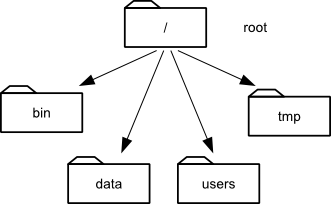
\includegraphics{novice/shell/img/filesystem.png}

We know that our current working directory \texttt{/users/vlad} is
stored inside \texttt{/users} because \texttt{/users} is the first part
of its name. Similarly, we know that \texttt{/users} is stored inside
the root directory \texttt{/} because its name begins with \texttt{/}.

Underneath \texttt{/users}, we find one directory for each user with an
account on this machine. The Mummy's files are stored in
\texttt{/users/imhotep}, Wolfman's in \texttt{/users/larry}, and ours in
\texttt{/users/vlad}, which is why \texttt{vlad} is the last part of the
directory's name.

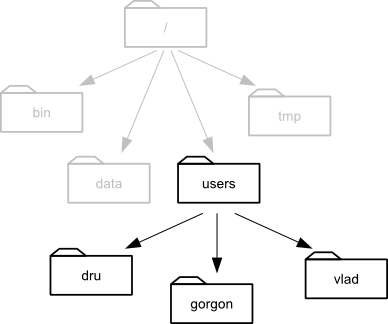
\includegraphics{novice/shell/img/home-directories.png}

\begin{quote}
Notice that there are two meanings for the \texttt{/} character. When it
appears at the front of a file or directory name, it refers to the root
directory. When it appears \emph{inside} a name, it's just a separator.
\end{quote}

Let's see what's in Vlad's home directory by running \texttt{ls}, which
stands for ``listing'':

\begin{verbatim}
$ ls
\end{verbatim}

\begin{verbatim}
bin          data      mail       music
notes.txt    papers    pizza.cfg  solar
solar.pdf    swc
\end{verbatim}

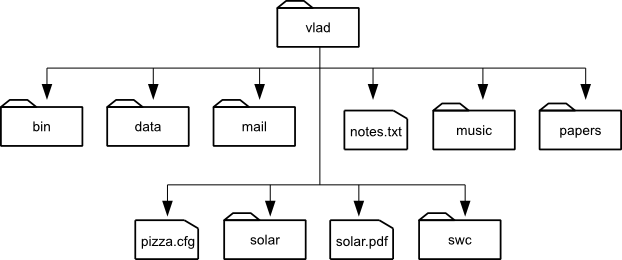
\includegraphics{novice/shell/img/vlad-homedir.png}

\texttt{ls} prints the names of the files and directories in the current
directory in alphabetical order, arranged neatly into columns. We can
make its output more comprehensible by using the
\gl{flag}{g:command-line-flag} \texttt{-F}, which tells
\texttt{ls} to add a trailing \texttt{/} to the names of directories:

\begin{verbatim}
$ ls -F
\end{verbatim}

\begin{verbatim}
bin/         data/     mail/      music/
notes.txt    papers/   pizza.cfg  solar/
solar.pdf    swc/
\end{verbatim}

Here, we can see that \texttt{/users/vlad} contains seven
\gl{sub-directories}{g:sub-directory}. The names that don't have
trailing slashes, like \texttt{notes.txt}, \texttt{pizza.cfg}, and
\texttt{solar.pdf}, are plain old files. And note that there is a space
between \texttt{ls} and \texttt{-F}: without it, the shell thinks we're
trying to run a command called \texttt{ls-F}, which doesn't exist.

\begin{swcbox}{What's In A Name?}

You may have noticed that all of Vlad's files' names are ``something dot
something''. This is just a convention: we can call a file
\texttt{mythesis} or almost anything else we want. However, most people
use two-part names most of the time to help them (and their programs)
tell different kinds of files apart. The second part of such a name is
called the \gl{filename extension}{g:filename-extension}, and
indicates what type of data the file holds: \texttt{.txt} signals a
plain text file, \texttt{.pdf} indicates a PDF document, \texttt{.cfg}
is a configuration file full of parameters for some program or other,
and so on.

This is just a convention, albeit an important one. Files contain bytes:
it's up to us and our programs to interpret those bytes according to the
rules for PDF documents, images, and so on.

Naming a PNG image of a whale as \texttt{whale.mp3} doesn't somehow
magically turn it into a recording of whalesong, though it \emph{might}
cause the operating system to try to open it with a music player when
someone double-clicks it.

\end{swcbox}

Now let's take a look at what's in Vlad's \texttt{data} directory by
running \texttt{ls -F data}, i.e., the command \texttt{ls} with the
parameters \texttt{-F} and \texttt{data}. The second parameter---the one
\emph{without} a leading dash---tells \texttt{ls} that we want a listing
of something other than our current working directory:

\begin{verbatim}
$ ls -F data
\end{verbatim}

\begin{verbatim}
amino-acids.txt   elements/     morse.txt
pdb/              planets.txt   sunspot.txt
\end{verbatim}

The output shows us that there are four text files and two
sub-sub-directories. Organizing things hierarchically in this way helps
us keep track of our work: it's possible to put hundreds of files in our
home directory, just as it's possible to pile hundreds of printed papers
on our desk, but it's a self-defeating strategy.

Notice, by the way that we spelled the directory name \texttt{data}. It
doesn't have a trailing slash: that's added to directory names by
\texttt{ls} when we use the \texttt{-F} flag to help us tell things
apart. And it doesn't begin with a slash because it's a
\gl{relative path}{g:relative-path}, i.e., it tells \texttt{ls}
how to find something from where we are, rather than from the root of
the file system.

If we run \texttt{ls -F /data} (\emph{with} a leading slash) we get a
different answer, because \texttt{/data} is an
\gl{absolute path}{g:absolute-path}:

\begin{verbatim}
$ ls -F /data
\end{verbatim}

\begin{verbatim}
access.log    backup/    hardware.cfg
network.cfg
\end{verbatim}

The leading \texttt{/} tells the computer to follow the path from the
root of the filesystem, so it always refers to exactly one directory, no
matter where we are when we run the command.

What if we want to change our current working directory? Before we do
this, \texttt{pwd} shows us that we're in \texttt{/users/vlad}, and
\texttt{ls} without any parameters shows us that directory's contents:

\begin{verbatim}
$ pwd
\end{verbatim}

\begin{verbatim}
/users/vlad
\end{verbatim}

\begin{verbatim}
$ ls
\end{verbatim}

\begin{verbatim}
bin/         data/     mail/      music/
notes.txt    papers/   pizza.cfg  solar/
solar.pdf    swc/
\end{verbatim}

We can use \texttt{cd} followed by a directory name to change our
working directory. \texttt{cd} stands for ``change directory'', which is
a bit misleading: the command doesn't change the directory, it changes
the shell's idea of what directory we are in.

\begin{verbatim}
$ cd data
\end{verbatim}

\texttt{cd} doesn't print anything, but if we run \texttt{pwd} after it,
we can see that we are now in \texttt{/users/vlad/data}. If we run
\texttt{ls} without parameters now, it lists the contents of
\texttt{/users/vlad/data}, because that's where we now are:

\begin{verbatim}
$ pwd
\end{verbatim}

\begin{verbatim}
/users/vlad/data
\end{verbatim}

\begin{verbatim}
$ ls
\end{verbatim}

\begin{verbatim}
amino-acids.txt   elements/     morse.txt
pdb/              planets.txt   sunspot.txt
\end{verbatim}

We now know how to go down the directory tree: how do we go up? We could
use an absolute path:

\begin{verbatim}
$ cd /users/vlad
\end{verbatim}

but it's almost always simpler to use \texttt{cd ..} to go up one level:

\begin{verbatim}
$ pwd
\end{verbatim}

\begin{verbatim}
/users/vlad/data
\end{verbatim}

\begin{verbatim}
$ cd ..
\end{verbatim}

\texttt{..} is a special directory name meaning ``the directory
containing this one'', or more succinctly, the
\gl{parent}{g:parent-directory} of the current directory. Sure
enough, if we run \texttt{pwd} after running \texttt{cd ..}, we're back
in \texttt{/users/vlad}:

\begin{verbatim}
$ pwd
\end{verbatim}

\begin{verbatim}
/users/vlad
\end{verbatim}

The special directory \texttt{..} doesn't usually show up when we run
\texttt{ls}. If we want to display it, we can give \texttt{ls} the
\texttt{-a} flag:

\begin{verbatim}
$ ls -F -a
\end{verbatim}

\begin{verbatim}
./           ../       bin/       data/
mail/        music/    notes.txt  papers/
pizza.cfg    solar/    solar.pdf    swc/
\end{verbatim}

\texttt{-a} stands for ``show all''; it forces \texttt{ls} to show us
file and directory names that begin with \texttt{.}, such as \texttt{..}
(which, if we're in \texttt{/users/vlad}, refers to the \texttt{/users}
directory). As you can see, it also displays another special directory
that's just called \texttt{.}, which means ``the current working
directory''. It may seem redundant to have a name for it, but we'll see
some uses for it soon.

\begin{swcbox}{Orthogonality}

The special names \texttt{.} and \texttt{..} don't belong to
\texttt{ls}; they are interpreted the same way by every program. For
example, if we are in \texttt{/users/vlad/data}, the command
\texttt{ls ..} will give us a listing of \texttt{/users/vlad}. When the
meanings of the parts are the same no matter how they're combined,
programmers say they are \gl{orthogonal}{g:orthogonal}: Orthogonal
systems tend to be easier for people to learn because there are fewer
special cases and exceptions to keep track of.

\end{swcbox}

\mbox{}\paragraph{Nelle's Pipeline: Organizing Files}

Knowing just this much about files and directories, Nelle is ready to
organize the files that the protein assay machine will create. First,
she creates a directory called \texttt{north-pacific-gyre} (to remind
herself where the data came from). Inside that, she creates a directory
called \texttt{2012-07-03}, which is the date she started processing the
samples. She used to use names like \texttt{conference-paper} and
\texttt{revised-results}, but she found them hard to understand after a
couple of years. (The final straw was when she found herself creating a
directory called \texttt{revised-revised-results-3}.)

\begin{quote}
Nelle names her directories ``year-month-day'', with leading zeroes for
months and days, because the shell displays file and directory names in
alphabetical order. If she used month names, December would come before
July; if she didn't use leading zeroes, November ('11') would come
before July ('7').
\end{quote}

Each of her physical samples is labelled according to her lab's
convention with a unique ten-character ID, such as ``NENE01729A''. This
is what she used in her collection log to record the location, time,
depth, and other characteristics of the sample, so she decides to use it
as part of each data file's name. Since the assay machine's output is
plain text, she will call her files \texttt{NENE01729A.txt},
\texttt{NENE01812A.txt}, and so on. All 1520 files will go into the same
directory.

If she is in her home directory, Nelle can see what files she has using
the command:

\begin{verbatim}
$ ls north-pacific-gyre/2012-07-03/
\end{verbatim}

This is a lot to type, but she can let the shell do most of the work. If
she types:

\begin{verbatim}
$ ls no
\end{verbatim}

and then presses tab, the shell automatically completes the directory
name for her:

\begin{verbatim}
$ ls north-pacific-gyre/
\end{verbatim}

If she presses tab again, Bash will add \texttt{2012-07-03/} to the
command, since it's the only possible completion. Pressing tab again
does nothing, since there are 1520 possibilities; pressing tab twice
brings up a list of all the files, and so on. This is called
\gl{tab completion}{g:tab-completion}, and we will see it in many
other tools as we go on.

\begin{keypoints}
\begin{swcitemize}
\item
  The file system is responsible for managing information on the disk.
\item
  Information is stored in files, which are stored in directories
  (folders).
\item
  Directories can also store other directories, which forms a directory
  tree.
\item
  \texttt{/} on its own is the root directory of the whole filesystem.
\item
  A relative path specifies a location starting from the current
  location.
\item
  An absolute path specifies a location from the root of the filesystem.
\item
  Directory names in a path are separated with `/' on Unix, but
  `\textbackslash{}' on Windows.
\item
  `..' means ``the directory above the current one''; `.' on its own
  means ``the current directory''.
\item
  Most files' names are \texttt{something.extension}. The extension
  isn't required, and doesn't guarantee anything, but is normally used
  to indicate the type of data in the file.
\item
  Most commands take options (flags) which begin with a `-'.
\end{swcitemize}
\end{keypoints}

Please refer to the diagram below for the following challenges:

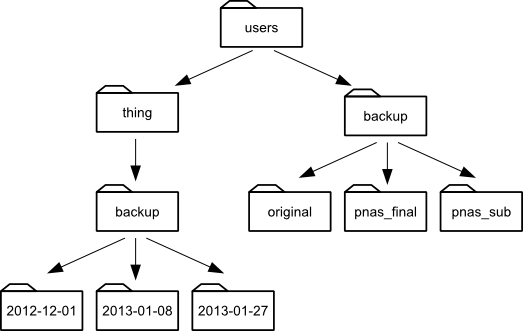
\includegraphics{novice/shell/img/filesystem-challenge.png}

\begin{challenge}

  If \texttt{pwd} displays \texttt{/users/thing}, what will
  \texttt{ls ../backup} display? 1.
  \texttt{../backup: No such file or directory} 2.
  \texttt{2012-12-01 2013-01-08 2013-01-27} 3.
  \texttt{2012-12-01/ 2013-01-08/ 2013-01-27/} 4.
  \texttt{original pnas\_final pnas\_sub}

\end{challenge}

\begin{challenge}

  If \texttt{pwd} displays \texttt{/users/backup}, and \texttt{-r} tells
  \texttt{ls} to display things in reverse order, what command will
  display:

\begin{verbatim}
pnas-sub/ pnas-final/ original/
\end{verbatim}

\begin{swcenumerate}
\item
  \texttt{ls pwd}
\item
  \texttt{ls -r -F}
\item
  \texttt{ls -r -F /users/backup}
\item
  Either \#2 or \#3 above, but not \#1.
\end{swcenumerate}

\end{challenge}

\begin{challenge}

  What does the command \texttt{cd} without a directory name do? 1. It has
  no effect. 2. It changes the working directory to \texttt{/}. 3. It
  changes the working directory to the user's home directory. 4. It
  produces an error message.

\end{challenge}

\begin{challenge}

  What does the command \texttt{ls} do when used with the -s and -h
  arguments?

\end{challenge}

\section{Creating Things}

\begin{objectives}
\begin{swcitemize}
\item
  Create a directory hierarchy that matches a given diagram.
\item
  Create files in that hierarchy using an editor or by copying and
  renaming existing files.
\item
  Display the contents of a directory using the command line.
\item
  Delete specified files and/or directories.
\end{swcitemize}
\end{objectives}

We now know how to explore files and directories, but how do we create
them in the first place? Let's go back to Vlad's home directory,
\texttt{/users/vlad}, and use \texttt{ls -F} to see what it contains:

\begin{verbatim}
$ pwd
\end{verbatim}

\begin{verbatim}
/users/vlad
\end{verbatim}

\begin{verbatim}
$ ls -F
\end{verbatim}

\begin{verbatim}
bin/         data/     mail/      music/
notes.txt    papers/   pizza.cfg  solar/
solar.pdf    swc/
\end{verbatim}

Let's create a new directory called \texttt{thesis} using the command
\texttt{mkdir thesis} (which has no output):

\begin{verbatim}
$ mkdir thesis
\end{verbatim}

As you might (or might not) guess from its name, \texttt{mkdir} means
``make directory''. Since \texttt{thesis} is a relative path (i.e.,
doesn't have a leading slash), the new directory is made below the
current working directory:

\begin{verbatim}
$ ls -F
\end{verbatim}

\begin{verbatim}
bin/         data/     mail/      music/
notes.txt    papers/   pizza.cfg  solar/
solar.pdf    swc/      thesis/
\end{verbatim}

However, there's nothing in it yet:

\begin{verbatim}
$ ls -F thesis
\end{verbatim}

Let's change our working directory to \texttt{thesis} using \texttt{cd},
then run a text editor called Nano to create a file called
\texttt{draft.txt}:

\begin{verbatim}
$ cd thesis
$ nano draft.txt
\end{verbatim}

\begin{swcbox}{Which Editor?}

When we say, ``\texttt{nano} is a text editor'' we really do mean
``text'': it can only work with plain character data, not tables,
images, or any other human-friendly media. We use it in examples because
almost anyone can drive it anywhere without training, but please use
something more powerful for real work. On Unix systems (such as Linux
and Mac OS X), many programmers use
\urlfoot{http://www.gnu.org/software/emacs/}{Emacs} or
\urlfoot{http://www.vim.org/}{Vim} (both of which are completely
unintuitive, even by Unix standards), or a graphical editor such as
\urlfoot{http://projects.gnome.org/gedit/}{Gedit}. On Windows, you may wish
to use \urlfoot{http://notepad-plus-plus.org/}{Notepad++}.

No matter what editor you use, you will need to know where it searches
for and saves files. If you start it from the shell, it will (probably)
use your current working directory as its default location. If you use
your computer's start menu, it may want to save files in your desktop or
documents directory instead. You can change this by navigating to
another directory the first time you ``Save As\ldots{}''

\end{swcbox}

Let's type in a few lines of text, then use Control-O to write our data
to disk:

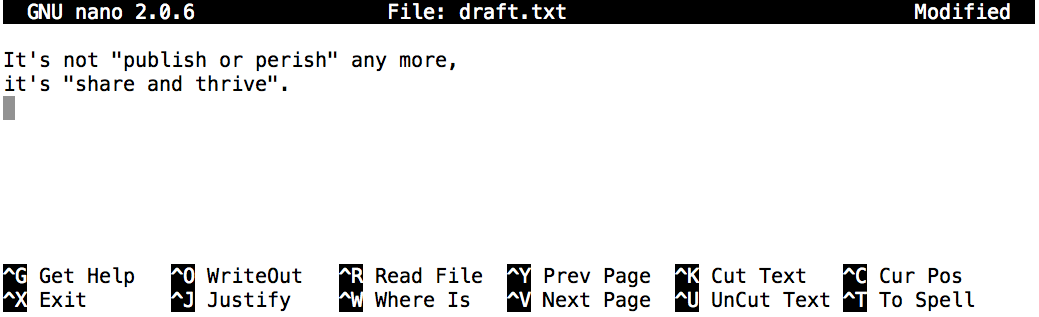
\includegraphics{novice/shell/img/nano-screenshot.png}

Once our file is saved, we can use Control-X to quit the editor and
return to the shell. (Unix documentation often uses the shorthand
\texttt{\^{}A} to mean ``control-A''.) \texttt{nano} doesn't leave any
output on the screen after it exits, but \texttt{ls} now shows that we
have created a file called \texttt{draft.txt}:

\begin{verbatim}
$ ls
\end{verbatim}

\begin{verbatim}
draft.txt
\end{verbatim}

Let's tidy up by running \texttt{rm draft.txt}:

\begin{verbatim}
$ rm draft.txt
\end{verbatim}

This command removes files (``rm'' is short for ``remove''). If we run
\texttt{ls} again, its output is empty once more, which tells us that
our file is gone:

\begin{verbatim}
$ ls
\end{verbatim}

\begin{swcbox}{Deleting Is Forever}

Unix doesn't have a trash bin: when we delete files, they are unhooked
from the file system so that their storage space on disk can be
recycled. Tools for finding and recovering deleted files do exist, but
there's no guarantee they'll work in any particular situation, since the
computer may recycle the file's disk space right away.

\end{swcbox}

Let's re-create that file and then move up one directory to
\texttt{/users/vlad} using \texttt{cd ..}:

\begin{verbatim}
$ pwd
\end{verbatim}

\begin{verbatim}
/users/vlad/thesis
\end{verbatim}

\begin{verbatim}
$ nano draft.txt
$ ls
\end{verbatim}

\begin{verbatim}
draft.txt
\end{verbatim}

\begin{verbatim}
$ cd ..
\end{verbatim}

If we try to remove the entire \texttt{thesis} directory using
\texttt{rm thesis}, we get an error message:

\begin{verbatim}
$ rm thesis
\end{verbatim}

\begin{verbatim}
rm: cannot remove `thesis': Is a directory
\end{verbatim}

This happens because \texttt{rm} only works on files, not directories.
The right command is \texttt{rmdir}, which is short for ``remove
directory''. It doesn't work yet either, though, because the directory
we're trying to remove isn't empty:

\begin{verbatim}
$ rmdir thesis
\end{verbatim}

\begin{verbatim}
rmdir: failed to remove `thesis': Directory not empty
\end{verbatim}

This little safety feature can save you a lot of grief, particularly if
you are a bad typist. To really get rid of \texttt{thesis} we must first
delete the file \texttt{draft.txt}:

\begin{verbatim}
$ rm thesis/draft.txt
\end{verbatim}

The directory is now empty, so \texttt{rmdir} can delete it:

\begin{verbatim}
$ rmdir thesis
\end{verbatim}

\begin{swcbox}{With Great Power Comes Great Responsibility}

Removing the files in a directory just so that we can remove the
directory quickly becomes tedious. Instead, we can use \texttt{rm} with
the \texttt{-r} flag (which stands for ``recursive''):

\begin{verbatim}
$ rm -r thesis
\end{verbatim}

This removes everything in the directory, then the directory itself. If
the directory contains sub-directories, \texttt{rm -r} does the same
thing to them, and so on. It's very handy, but can do a lot of damage if
used without care.

\end{swcbox}

Let's create that directory and file one more time. (Note that this time
we're running \texttt{nano} with the path \texttt{thesis/draft.txt},
rather than going into the \texttt{thesis} directory and running
\texttt{nano} on \texttt{draft.txt} there.)

\begin{verbatim}
$ pwd
\end{verbatim}

\begin{verbatim}
/users/vlad
\end{verbatim}

\begin{verbatim}
$ mkdir thesis
\end{verbatim}

\begin{verbatim}
$ nano thesis/draft.txt
$ ls thesis
\end{verbatim}

\begin{verbatim}
draft.txt
\end{verbatim}

\texttt{draft.txt} isn't a particularly informative name, so let's
change the file's name using \texttt{mv}, which is short for ``move'':

\begin{verbatim}
$ mv thesis/draft.txt thesis/quotes.txt
\end{verbatim}

The first parameter tells \texttt{mv} what we're ``moving'', while the
second is where it's to go. In this case, we're moving
\texttt{thesis/draft.txt} to \texttt{thesis/quotes.txt}, which has the
same effect as renaming the file. Sure enough, \texttt{ls} shows us that
\texttt{thesis} now contains one file called \texttt{quotes.txt}:

\begin{verbatim}
$ ls thesis
\end{verbatim}

\begin{verbatim}
quotes.txt
\end{verbatim}

Just for the sake of inconsistency, \texttt{mv} also works on
directories---there is no separate \texttt{mvdir} command.

Let's move \texttt{quotes.txt} into the current working directory. We
use \texttt{mv} once again, but this time we'll just use the name of a
directory as the second parameter to tell \texttt{mv} that we want to
keep the filename, but put the file somewhere new. (This is why the
command is called ``move''.) In this case, the directory name we use is
the special directory name \texttt{.} that we mentioned earlier.

\begin{verbatim}
$ mv thesis/quotes.txt .
\end{verbatim}

The effect is to move the file from the directory it was in to the
current working directory. \texttt{ls} now shows us that \texttt{thesis}
is empty:

\begin{verbatim}
$ ls thesis
\end{verbatim}

Further, \texttt{ls} with a filename or directory name as a parameter
only lists that file or directory. We can use this to see that
\texttt{quotes.txt} is still in our current directory:

\begin{verbatim}
$ ls quotes.txt
\end{verbatim}

\begin{verbatim}
quotes.txt
\end{verbatim}

The \texttt{cp} command works very much like \texttt{mv}, except it
copies a file instead of moving it. We can check that it did the right
thing using \texttt{ls} with two paths as parameters---like most Unix
commands, \texttt{ls} can be given thousands of paths at once:

\begin{verbatim}
$ cp quotes.txt thesis/quotations.txt
$ ls quotes.txt thesis/quotations.txt
\end{verbatim}

\begin{verbatim}
quotes.txt   thesis/quotations.txt
\end{verbatim}

To prove that we made a copy, let's delete the \texttt{quotes.txt} file
in the current directory and then run that same \texttt{ls} again. This
time it tells us that it can't find \texttt{quotes.txt} in the current
directory, but it does find the copy in \texttt{thesis} that we didn't
delete:

\begin{verbatim}
$ ls quotes.txt thesis/quotations.txt
\end{verbatim}

\begin{verbatim}
ls: cannot access quotes.txt: No such file or directory
thesis/quotations.txt
\end{verbatim}

\begin{swcbox}{Another Useful Abbreviation}

The shell interprets the character \texttt{\textasciitilde{}} (tilde) at
the start of a path to mean ``the current user's home directory''. For
example, if Vlad's home directory is \texttt{/home/vlad}, then
\texttt{\textasciitilde{}/data} is equivalent to
\texttt{/home/vlad/data}. This only works if it is the first character
in the path: \texttt{here/there/\textasciitilde{}/elsewhere} is
\emph{not} \texttt{/home/vlad/elsewhere}.

\end{swcbox}

\begin{keypoints}
\begin{swcitemize}
\item
  Unix documentation uses `\^{}A' to mean ``control-A''.
\item
  The shell does not have a trash bin: once something is deleted, it's
  really gone.
\item
  Nano is a very simple text editor---please use something else for real
  work.
\end{swcitemize}
\end{keypoints}

\begin{challenge}
  What is the output of the closing \texttt{ls} command in the sequence
  shown below?

\begin{verbatim}
$ pwd
/home/thing/data
$ ls
proteins.dat
$ mkdir recombine
$ mv proteins.dat recombine
$ cp recombine/proteins.dat ../proteins-saved.dat
$ ls
\end{verbatim}
\end{challenge}

\begin{challenge}
  Suppose that:

\begin{verbatim}
$ ls -F
analyzed/  fructose.dat    raw/   sucrose.dat
\end{verbatim}

  What command(s) could you run so that the commands below will produce
  the output shown?

\begin{verbatim}
$ ls
analyzed   raw
$ ls analyzed
fructose.dat    sucrose.dat
\end{verbatim}
\end{challenge}

\begin{challenge}
  What does \texttt{cp} do when given several filenames and a directory
  name, as in:

\begin{verbatim}
$ mkdir backup
$ cp thesis/citations.txt thesis/quotations.txt backup
\end{verbatim}

  What does \texttt{cp} do when given three or more filenames, as in:

\begin{verbatim}
$ ls -F
intro.txt    methods.txt    survey.txt
$ cp intro.txt methods.txt survey.txt
\end{verbatim}
\end{challenge}

\begin{challenge}
  The command \texttt{ls -R} lists the contents of directories
  recursively, i.e., lists their sub-directories, sub-sub-directories,
  and so on in alphabetical order at each level. The command
  \texttt{ls -t} lists things by time of last change, with most recently
  changed files or directories first. In what order does
  \texttt{ls -R -t} display things?
\end{challenge}

\section{Pipes and Filters}

\begin{objectives}
\begin{swcitemize}
\item
  Redirect a command's output to a file.
\item
  Process a file instead of keyboard input using redirection.
\item
  Construct command pipelines with two or more stages.
\item
  Explain what usually happens if a program or pipeline isn't given any
  input to process.
\item
  Explain Unix's ``small pieces, loosely joined'' philosophy.
\end{swcitemize}
\end{objectives}

Now that we know a few basic commands, we can finally look at the
shell's most powerful feature: the ease with which it lets us combine
existing programs in new ways. We'll start with a directory called
\texttt{molecules} that contains six files describing some simple
organic molecules. The \texttt{.pdb} extension indicates that these
files are in Protein Data Bank format, a simple text format that
specifies the type and position of each atom in the molecule.

\begin{verbatim}
$ ls molecules
\end{verbatim}

\begin{verbatim}
cubane.pdb    ethane.pdb    methane.pdb
octane.pdb    pentane.pdb   propane.pdb
\end{verbatim}

Let's go into that directory with \texttt{cd} and run the command
\texttt{wc *.pdb}. \texttt{wc} is the ``word count'' command: it counts
the number of lines, words, and characters in files. The \texttt{*} in
\texttt{*.pdb} matches zero or more characters, so the shell turns
\texttt{*.pdb} into a complete list of \texttt{.pdb} files:

\begin{verbatim}
$ cd molecules
$ wc *.pdb
\end{verbatim}

\begin{verbatim}
  20  156 1158 cubane.pdb
  12   84  622 ethane.pdb
   9   57  422 methane.pdb
  30  246 1828 octane.pdb
  21  165 1226 pentane.pdb
  15  111  825 propane.pdb
 107  819 6081 total
\end{verbatim}

\begin{swcbox}{Wildcards}

\texttt{*} is a \gl{wildcard}{g:wildcard}. It matches zero or more
characters, so \texttt{*.pdb} matches \texttt{ethane.pdb},
\texttt{propane.pdb}, and so on. On the other hand, \texttt{p*.pdb} only
matches \texttt{pentane.pdb} and \texttt{propane.pdb}, because the `p'
at the front only matches itself.

\texttt{?} is also a wildcard, but it only matches a single character.
This means that \texttt{p?.pdb} matches \texttt{pi.pdb} or
\texttt{p5.pdb}, but not \texttt{propane.pdb}. We can use any number of
wildcards at a time: for example, \texttt{p*.p?*} matches anything that
starts with a `p' and ends with `.', `p', and at least one more
character (since the `?' has to match one character, and the final `*'
can match any number of characters). Thus, \texttt{p*.p?*} would match
\texttt{preferred.practice}, and even \texttt{p.pi} (since the first `*'
can match no characters at all), but not \texttt{quality.practice}
(doesn't start with `p') or \texttt{preferred.p} (there isn't at least
one character after the `.p').

When the shell sees a wildcard, it expands the wildcard to create a list
of matching filenames \emph{before} running the command that was asked
for. This means that commands like \texttt{wc} and \texttt{ls} never see
the wildcard characters, just what those wildcards matched. This is
another example of orthogonal design.

\end{swcbox}

If we run \texttt{wc -l} instead of just \texttt{wc}, the output shows
only the number of lines per file:

\begin{verbatim}
$ wc -l *.pdb
\end{verbatim}

\begin{verbatim}
  20  cubane.pdb
  12  ethane.pdb
   9  methane.pdb
  30  octane.pdb
  21  pentane.pdb
  15  propane.pdb
 107  total
\end{verbatim}

We can also use \texttt{-w} to get only the number of words, or
\texttt{-c} to get only the number of characters.

Which of these files is shortest? It's an easy question to answer when
there are only six files, but what if there were 6000? Our first step
toward a solution is to run the command:

\begin{verbatim}
$ wc -l *.pdb > lengths
\end{verbatim}

The \texttt{\textgreater{}} tells the shell to
\gl{redirect}{g:redirect} the command's output to a file instead
of printing it to the screen. The shell will create the file if it
doesn't exist, or overwrite the contents of that file if it does. (This
is why there is no screen output: everything that \texttt{wc} would have
printed has gone into the file \texttt{lengths} instead.)
\texttt{ls lengths} confirms that the file exists:

\begin{verbatim}
$ ls lengths
\end{verbatim}

\begin{verbatim}
lengths
\end{verbatim}

We can now send the content of \texttt{lengths} to the screen using
\texttt{cat lengths}. \texttt{cat} stands for ``concatenate'': it prints
the contents of files one after another. There's only one file in this
case, so \texttt{cat} just shows us what it contains:

\begin{verbatim}
$ cat lengths
\end{verbatim}

\begin{verbatim}
  20  cubane.pdb
  12  ethane.pdb
   9  methane.pdb
  30  octane.pdb
  21  pentane.pdb
  15  propane.pdb
 107  total
\end{verbatim}

Now let's use the \texttt{sort} command to sort its contents. This does
\emph{not} change the file; instead, it sends the sorted result to the
screen:

\begin{verbatim}
$ sort lengths
\end{verbatim}

\begin{verbatim}
  9  methane.pdb
 12  ethane.pdb
 15  propane.pdb
 20  cubane.pdb
 21  pentane.pdb
 30  octane.pdb
107  total
\end{verbatim}

We can put the sorted list of lines in another temporary file called
\texttt{sorted-lengths} by putting
\texttt{\textgreater{} sorted-lengths} after the command, just as we
used \texttt{\textgreater{} lengths} to put the output of \texttt{wc}
into \texttt{lengths}. Once we've done that, we can run another command
called \texttt{head} to get the first few lines in
\texttt{sorted-lengths}:

\begin{verbatim}
$ sort lengths > sorted-lengths
$ head -1 sorted-lengths
\end{verbatim}

\begin{verbatim}
  9  methane.pdb
\end{verbatim}

Using the parameter \texttt{-1} with \texttt{head} tells it that we only
want the first line of the file; \texttt{-20} would get the first 20,
and so on. Since \texttt{sorted-lengths} contains the lengths of our
files ordered from least to greatest, the output of \texttt{head} must
be the file with the fewest lines.

If you think this is confusing, you're in good company: even once you
understand what \texttt{wc}, \texttt{sort}, and \texttt{head} do, all
those intermediate files make it hard to follow what's going on. We can
make it easier to understand by running \texttt{sort} and \texttt{head}
together:

\begin{verbatim}
$ sort lengths | head -1
\end{verbatim}

\begin{verbatim}
  9  methane.pdb
\end{verbatim}

The vertical bar between the two commands is called a
\gl{pipe}{g:pipe}. It tells the shell that we want to use the
output of the command on the left as the input to the command on the
right. The computer might create a temporary file if it needs to, or
copy data from one program to the other in memory, or something else
entirely; we don't have to know or care.

We can use another pipe to send the output of \texttt{wc} directly to
\texttt{sort}, which then sends its output to \texttt{head}:

\begin{verbatim}
$ wc -l *.pdb | sort | head -1
\end{verbatim}

\begin{verbatim}
  9  methane.pdb
\end{verbatim}

This is exactly like a mathematician nesting functions like
\emph{sin($\pi$x)\textsuperscript{2}} and saying ``the square of the sine of
\emph{x} times $\pi$''. In our case, the calculation is ``head of sort of
word count of \texttt{*.pdb}''.

Here's what actually happens behind the scenes when we create a pipe.
When a computer runs a program---any program---it creates a
\gl{process}{g:process} in memory to hold the program's software
and its current state. Every process has an input channel called
\gl{standard input}{g:standard-input}. (By this point, you may be
surprised that the name is so memorable, but don't worry: most Unix
programmers call it ``stdin''. Every process also has a default output
channel called \gl{standard output}{g:standard-output} (or
``stdout'').

The shell is actually just another program. Under normal circumstances,
whatever we type on the keyboard is sent to the shell on its standard
input, and whatever it produces on standard output is displayed on our
screen. When we tell the shell to run a program, it creates a new
process and temporarily sends whatever we type on our keyboard to that
process's standard input, and whatever the process sends to standard
output to the screen.

Here's what happens when we run
\texttt{wc -l *.pdb \textgreater{} lengths}. The shell starts by telling
the computer to create a new process to run the \texttt{wc} program.
Since we've provided some filenames as parameters, \texttt{wc} reads
from them instead of from standard input. And since we've used
\texttt{\textgreater{}} to redirect output to a file, the shell connects
the process's standard output to that file.

If we run \texttt{wc -l *.pdb \textbar{} sort} instead, the shell
creates two processes (one for each process in the pipe) so that
\texttt{wc} and \texttt{sort} run simultaneously. The standard output of
\texttt{wc} is fed directly to the standard input of \texttt{sort};
since there's no redirection with \texttt{\textgreater{}},
\texttt{sort}'s output goes to the screen. And if we run
\texttt{wc -l *.pdb \textbar{} sort \textbar{} head -1}, we get three
processes with data flowing from the files, through \texttt{wc} to
\texttt{sort}, and from \texttt{sort} through \texttt{head} to the
screen.

This simple idea is why Unix has been so successful. Instead of creating
enormous programs that try to do many different things, Unix programmers
focus on creating lots of simple tools that each do one job well, and
that work well with each other. This programming model is called
\gl{pipes and filters}{g:pipe-and-filter}. We've already seen
pipes; a \gl{filter}{g:filter} is a program like \texttt{wc} or
\texttt{sort} that transforms a stream of input into a stream of output.
Almost all of the standard Unix tools can work this way: unless told to
do otherwise, they read from standard input, do something with what
they've read, and write to standard output.

The key is that any program that reads lines of text from standard input
and writes lines of text to standard output can be combined with every
other program that behaves this way as well. You can \emph{and should}
write your programs this way so that you and other people can put those
programs into pipes to multiply their power.

\begin{swcbox}{Redirecting Input}

As well as using \texttt{\textgreater{}} to redirect a program's output,
we can use \texttt{\textless{}} to redirect its input, i.e., to read
from a file instead of from standard input. For example, instead of
writing \texttt{wc ammonia.pdb}, we could write
\texttt{wc \textless{} ammonia.pdb}. In the first case, \texttt{wc} gets
a command line parameter telling it what file to open. In the second,
\texttt{wc} doesn't have any command line parameters, so it reads from
standard input, but we have told the shell to send the contents of
\texttt{ammonia.pdb} to \texttt{wc}'s standard input.

\end{swcbox}

\mbox{}\paragraph{Nelle's Pipeline: Checking Files}

Nelle has run her samples through the assay machines and created 1520
files in the \texttt{north-pacific-gyre/2012-07-03} directory described
earlier. As a quick sanity check, she types:

\begin{verbatim}
$ cd north-pacific-gyre/2012-07-03
$ wc -l *.txt
\end{verbatim}

The output is 1520 lines that look like this:

\begin{verbatim}
300 NENE01729A.txt
300 NENE01729B.txt
300 NENE01736A.txt
300 NENE01751A.txt
300 NENE01751B.txt
300 NENE01812A.txt
... ...
\end{verbatim}

Now she types this:

\begin{verbatim}
$ wc -l *.txt | sort | head -5
\end{verbatim}

\begin{verbatim}
 240 NENE02018B.txt
 300 NENE01729A.txt
 300 NENE01729B.txt
 300 NENE01736A.txt
 300 NENE01751A.txt
\end{verbatim}

Whoops: one of the files is 60 lines shorter than the others. When she
goes back and checks it, she sees that she did that assay at 8:00 on a
Monday morning---someone was probably in using the machine on the
weekend, and she forgot to reset it. Before re-running that sample, she
checks to see if any files have too much data:

\begin{verbatim}
$ wc -l *.txt | sort | tail -5
\end{verbatim}

\begin{verbatim}
 300 NENE02040A.txt
 300 NENE02040B.txt
 300 NENE02040Z.txt
 300 NENE02043A.txt
 300 NENE02043B.txt
\end{verbatim}

Those numbers look good---but what's that `Z' doing there in the
third-to-last line? All of her samples should be marked `A' or `B'; by
convention, her lab uses `Z' to indicate samples with missing
information. To find others like it, she does this:

\begin{verbatim}
$ ls *Z.txt
\end{verbatim}

\begin{verbatim}
NENE01971Z.txt    NENE02040Z.txt
\end{verbatim}

Sure enough, when she checks the log on her laptop, there's no depth
recorded for either of those samples. Since it's too late to get the
information any other way, she must exclude those two files from her
analysis. She could just delete them using \texttt{rm}, but there are
actually some analyses she might do later where depth doesn't matter, so
instead, she'll just be careful later on to select files using the
wildcard expression \texttt{*{[}AB{]}.txt}. As always, the `*' matches
any number of characters; the expression \texttt{{[}AB{]}} matches
either an `A' or a `B', so this matches all the valid data files she
has.

\begin{keypoints}
\begin{swcitemize}
\item
  \texttt{command \textgreater{} file} redirects a command's output to a
  file.
\item
  \texttt{first \textbar{} second} is a pipeline: the output of the
  first command is used as the input to the second.
\item
  The best way to use the shell is to use pipes to combine simple
  single-purpose programs (filters).
\end{swcitemize}
\end{keypoints}

\begin{challenge}
  If we run \texttt{sort} on this file:

\begin{verbatim}
10
2
19
22
6
\end{verbatim}

  the output is:

\begin{verbatim}
10
19
2
22
6
\end{verbatim}

  If we run \texttt{sort -n} on the same input, we get this instead:

\begin{verbatim}
2
6
10
19
22
\end{verbatim}

  Explain why \texttt{-n} has this effect.
\end{challenge}

\begin{challenge}
  What is the difference between:

\begin{verbatim}
wc -l < mydata.dat
\end{verbatim}

  and:

\begin{verbatim}
wc -l mydata.dat
\end{verbatim}
\end{challenge}

\begin{challenge}
  The command \texttt{uniq} removes adjacent duplicated lines from its
  input. For example, if a file \texttt{salmon.txt} contains:

\begin{verbatim}
coho
coho
steelhead
coho
steelhead
steelhead
\end{verbatim}

  then \texttt{uniq salmon.txt} produces:

\begin{verbatim}
coho
steelhead
coho
steelhead
\end{verbatim}

  Why do you think \texttt{uniq} only removes \emph{adjacent} duplicated
  lines? (Hint: think about very large data sets.) What other command
  could you combine with it in a pipe to remove all duplicated lines?
\end{challenge}

\begin{challenge}
  A file called \texttt{animals.txt} contains the following data:

\begin{verbatim}
2012-11-05,deer
2012-11-05,rabbit
2012-11-05,raccoon
2012-11-06,rabbit
2012-11-06,deer
2012-11-06,fox
2012-11-07,rabbit
2012-11-07,bear
\end{verbatim}

  What text passes through each of the pipes and the final redirect in
  the pipeline below?

\begin{verbatim}
cat animals.txt | head -5 | tail -3 | sort -r > final.txt
\end{verbatim}
\end{challenge}

\begin{challenge}
  The command:

\begin{verbatim}
$ cut -d , -f 2 animals.txt
\end{verbatim}

  produces the following output:

\begin{verbatim}
deer
rabbit
raccoon
rabbit
deer
fox
rabbit
bear
\end{verbatim}

  What other command(s) could be added to this in a pipeline to find out
  what animals the file contains (without any duplicates in their
  names)?
\end{challenge}

\section{Loops}

\begin{objectives}
\begin{swcitemize}
\item
  Write a loop that applies one or more commands separately to each file
  in a set of files.
\item
  Trace the values taken on by a loop variable during execution of the
  loop.
\item
  Explain the difference between a variable's name and its value.
\item
  Explain why spaces and some punctuation characters shouldn't be used
  in files' names.
\item
  Demonstrate how to see what commands have recently been executed.
\item
  Re-run recently executed commands without retyping them.
\end{swcitemize}
\end{objectives}

Wildcards and tab completion are two ways to reduce typing (and typing
mistakes). Another is to tell the shell to do something over and over
again. Suppose we have several hundred genome data files named
\texttt{basilisk.dat}, \texttt{unicorn.dat}, and so on. When new files
arrive, we'd like to rename the existing ones to
\texttt{original-basilisk.dat} and \texttt{original-unicorn.dat}. We
can't use:

\begin{verbatim}
$ mv *.dat original-*.dat
\end{verbatim}

because that would expand (in the two-file case) to:

\begin{verbatim}
$ mv basilisk.dat unicorn.dat
\end{verbatim}

This wouldn't back up our files: it would replace the content of
\texttt{unicorn.dat} with whatever's in \texttt{basilisk.dat}.

Instead, we can use a \gl{loop}{g:for-loop} to do some operation
once for each thing in a list. Here's a simple example that displays the
first three lines of each file in turn:

\begin{verbatim}
$ for filename in basilisk.dat unicorn.dat
> do
>    head -3 $filename
> done
\end{verbatim}

\begin{verbatim}
COMMON NAME: basilisk
CLASSIFICATION: basiliscus vulgaris
UPDATED: 1745-05-02
COMMON NAME: unicorn
CLASSIFICATION: equus monoceros
UPDATED: 1738-11-24
\end{verbatim}

When the shell sees the keyword \texttt{for}, it knows it is supposed to
repeat a command (or group of commands) once for each thing in a list.
In this case, the list is the two filenames. Each time through the loop,
the name of the thing currently being operated on is assigned to the
\gl{variable}{g:variable} called \texttt{filename}. Inside the
loop, we get the variable's value by putting \texttt{\$} in front of it:
\texttt{\$filename} is \texttt{basilisk.dat} the first time through the
loop, \texttt{unicorn.dat} the second, and so on. Finally, the command
that's actually being run is our old friend \texttt{head}, so this loop
prints out the first three lines of each data file in turn.

\begin{swcbox}{Follow the Prompt}

The shell prompt changes from \texttt{\$} to \texttt{\textgreater{}} and
back again as we were typing in our loop. The second prompt,
\texttt{\textgreater{}}, is different to remind us that we haven't
finished typing a complete command yet.

\end{swcbox}

We have called the variable in this loop \texttt{filename} in order to
make its purpose clearer to human readers. The shell itself doesn't care
what the variable is called; if we wrote this loop as:

\begin{verbatim}
for x in basilisk.dat unicorn.dat
do
    head -3 $x
done
\end{verbatim}

or:

\begin{verbatim}
for temperature in basilisk.dat unicorn.dat
do
    head -3 $temperature
done
\end{verbatim}

it would work exactly the same way. \emph{Don't do this.} Programs are
only useful if people can understand them, so meaningless names (like
\texttt{x}) or misleading names (like \texttt{temperature}) increase the
odds that the program won't do what its readers think it does.

Here's a slightly more complicated loop:

\begin{verbatim}
for filename in *.dat
do
    echo $filename
    head -100 $filename | tail -20
done
\end{verbatim}

The shell starts by expanding \texttt{*.dat} to create the list of files
it will process. The \gl{loop body}{g:loop-body} then executes two
commands for each of those files. The first, \texttt{echo}, just prints
its command-line parameters to standard output. For example:

\begin{verbatim}
$ echo hello there
\end{verbatim}

prints:

\begin{verbatim}
hello there
\end{verbatim}

In this case, since the shell expands \texttt{\$filename} to be the name
of a file, \texttt{echo \$filename} just prints the name of the file.
Note that we can't write this as:

\begin{verbatim}
for filename in *.dat
do
    $filename
    head -100 $filename | tail -20
done
\end{verbatim}

because then the first time through the loop, when \texttt{\$filename}
expanded to \texttt{basilisk.dat}, the shell would try to run
\texttt{basilisk.dat} as a program. Finally, the \texttt{head} and
\texttt{tail} combination selects lines 81-100 from whatever file is
being processed.

\begin{swcbox}{Spaces in Names}

Filename expansion in loops is another reason you should not use spaces
in filenames. Suppose our data files are named:

\begin{verbatim}
basilisk.dat
red dragon.dat
unicorn.dat
\end{verbatim}

If we try to process them using:

\begin{verbatim}
for filename in *.dat
do
    head -100 $filename | tail -20
done
\end{verbatim}

then the shell will expand \texttt{*.dat} to create:

\begin{verbatim}
basilisk.dat red dragon.dat unicorn.dat
\end{verbatim}

With older versions of Bash, or most other shells, \texttt{filename}
will then be assigned the following values in turn:

\begin{verbatim}
basilisk.dat
red
dragon.dat
unicorn.dat
\end{verbatim}

That's a problem: \texttt{head} can't read files called \texttt{red} and
\texttt{dragon.dat} because they don't exist, and won't be asked to read
the file \texttt{red dragon.dat}.

We can make our script a little bit more robust by
\gl{quoting}{g:shell-quoting} our use of the variable:

\begin{verbatim}
for filename in *.dat
do
    head -100 "$filename" | tail -20
done
\end{verbatim}

but it's simpler just to avoid using spaces (or other special
characters) in filenames.

\end{swcbox}

Going back to our original file renaming problem, we can solve it using
this loop:

\begin{verbatim}
for filename in *.dat
do
    mv $filename original-$filename
done
\end{verbatim}

This loop runs the \texttt{mv} command once for each filename. The first
time, when \texttt{\$filename} expands to \texttt{basilisk.dat}, the
shell executes:

\begin{verbatim}
mv basilisk.dat original-basilisk.dat
\end{verbatim}

The second time, the command is:

\begin{verbatim}
mv unicorn.dat original-unicorn.dat
\end{verbatim}

\begin{swcbox}{Measure Twice, Run Once}

A loop is a way to do many things at once---or to make many mistakes at
once if it does the wrong thing. One way to check what a loop
\emph{would} do is to echo the commands it would run instead of actually
running them. For example, we could write our file renaming loop like
this:

\begin{verbatim}
for filename in *.dat
do
    echo mv $filename original-$filename
done
\end{verbatim}

Instead of running \texttt{mv}, this loop runs \texttt{echo}, which
prints out:

\begin{verbatim}
mv basilisk.dat original-basilisk.dat
mv unicorn.dat original-unicorn.dat
\end{verbatim}

\emph{without} actually running those commands. We can then use up-arrow
to redisplay the loop, back-arrow to get to the word \texttt{echo},
delete it, and then press ``enter'' to run the loop with the actual
\texttt{mv} commands. This isn't foolproof, but it's a handy way to see
what's going to happen when you're still learning how loops work.

\end{swcbox}

\mbox{}\paragraph{Nelle's Pipeline: Processing Files}

Nelle is now ready to process her data files. Since she's still learning
how to use the shell, she decides to build up the required commands in
stages. Her first step is to make sure that she can select the right
files---remember, these are ones whose names end in `A' or `B', rather
than `Z':

\begin{verbatim}
$ cd north-pacific-gyre/2012-07-03
$ for datafile in *[AB].txt
> do
>     echo $datafile
> done
\end{verbatim}

\begin{verbatim}
NENE01729A.txt
NENE01729B.txt
NENE01736A.txt
...
NENE02043A.txt
NENE02043B.txt
\end{verbatim}

Her next step is to decide what to call the files that the
\texttt{goostats} analysis program will create. Prefixing each input
file's name with ``stats'' seems simple, so she modifies her loop to do
that:

\begin{verbatim}
$ for datafile in *[AB].txt
> do
>     echo $datafile stats-$datafile
> done
\end{verbatim}

\begin{verbatim}
NENE01729A.txt stats-NENE01729A.txt
NENE01729B.txt stats-NENE01729B.txt
NENE01736A.txt stats-NENE01736A.txt
...
NENE02043A.txt stats-NENE02043A.txt
NENE02043B.txt stats-NENE02043B.txt
\end{verbatim}

She hasn't actually run \texttt{goostats} yet, but now she's sure she
can select the right files and generate the right output filenames.

Typing in commands over and over again is becoming tedious, though, and
Nelle is worried about making mistakes, so instead of re-entering her
loop, she presses the up arrow. In response, the shell redisplays the
whole loop on one line (using semi-colons to separate the pieces):

\begin{verbatim}
$ for datafile in *[AB].txt; do echo $datafile stats-$datafile; done
\end{verbatim}

Using the left arrow key, Nelle backs up and changes the command
\texttt{echo} to \texttt{goostats}:

\begin{verbatim}
$ for datafile in *[AB].txt; do bash goostats $datafile stats-$datafile; done
\end{verbatim}

When she presses enter, the shell runs the modified command. However,
nothing appears to happen---there is no output. After a moment, Nelle
realizes that since her script doesn't print anything to the screen any
longer, she has no idea whether it is running, much less how quickly.
She kills the job by typing Control-C, uses up-arrow to repeat the
command, and edits it to read:

\begin{verbatim}
$ for datafile in *[AB].txt; do echo $datafile; bash goostats $datafile stats-$datafile; done
\end{verbatim}

\begin{swcbox}{Beginning and End}

We can move to the beginning of a line in the shell by typing
\texttt{\^{}A} (which means Control-A) and to the end using
\texttt{\^{}E}.

\end{swcbox}

When she runs her program now, it produces one line of output every five
seconds or so:

\begin{verbatim}
NENE01729A.txt
NENE01729B.txt
NENE01736A.txt
...
\end{verbatim}

1518 times 5 seconds, divided by 60, tells her that her script will take
about two hours to run. As a final check, she opens another terminal
window, goes into \texttt{north-pacific-gyre/2012-07-03}, and uses
\texttt{cat stats-NENE01729B.txt} to examine one of the output files. It
looks good, so she decides to get some coffee and catch up on her
reading.

\begin{swcbox}{Those Who Know History Can Choose to Repeat It}

Another way to repeat previous work is to use the \texttt{history}
command to get a list of the last few hundred commands that have been
executed, and then to use \texttt{!123} (where ``123'' is replaced by
the command number) to repeat one of those commands. For example, if
Nelle types this:

\begin{verbatim}
$ history | tail -5
  456  ls -l NENE0*.txt
  457  rm stats-NENE01729B.txt.txt
  458  bash goostats NENE01729B.txt stats-NENE01729B.txt
  459  ls -l NENE0*.txt
  460  history
\end{verbatim}

then she can re-run \texttt{goostats} on \texttt{NENE01729B.txt} simply
by typing \texttt{!458}.

\end{swcbox}

\begin{keypoints}
\begin{swcitemize}
\item
  A \texttt{for} loop repeats commands once for every thing in a list.
\item
  Every \texttt{for} loop needs a variable to refer to the current
  ``thing''.
\item
  Use \texttt{\$name} to expand a variable (i.e., get its value).
\item
  Do not use spaces, quotes, or wildcard characters such as `*' or `?'
  in filenames, as it complicates variable expansion.
\item
  Give files consistent names that are easy to match with wildcard
  patterns to make it easy to select them for looping.
\item
  Use the up-arrow key to scroll up through previous commands to edit
  and repeat them.
\item
  Use \texttt{history} to display recent commands, and \texttt{!number}
  to repeat a command by number.
\end{swcitemize}
\end{keypoints}

\begin{challenge}
  Suppose that \texttt{ls} initially displays:

\begin{verbatim}
fructose.dat    glucose.dat   sucrose.dat
\end{verbatim}

  What is the output of:

\begin{verbatim}
for datafile in *.dat
do
    ls *.dat
done
\end{verbatim}
\end{challenge}

\begin{challenge}
  In the same directory, what is the effect of this loop?

\begin{verbatim}
for sugar in *.dat
do
    echo $sugar
    cat $sugar > xylose.dat
done
\end{verbatim}

  \begin{swcenumerate}
  \item
    Prints \texttt{fructose.dat}, \texttt{glucose.dat}, and
    \texttt{sucrose.dat}, and copies \texttt{sucrose.dat} to create
    \texttt{xylose.dat}.
  \item
    Prints \texttt{fructose.dat}, \texttt{glucose.dat}, and
    \texttt{sucrose.dat}, and concatenates all three files to create
    \texttt{xylose.dat}.
  \item
    Prints \texttt{fructose.dat}, \texttt{glucose.dat},
    \texttt{sucrose.dat}, and \texttt{xylose.dat}, and copies
    \texttt{sucrose.dat} to create \texttt{xylose.dat}.
  \item
    None of the above.
  \end{swcenumerate}
\end{challenge}

\begin{challenge}
  The \texttt{expr} does simple arithmetic using command-line
  parameters:

\begin{verbatim}
$ expr 3 + 5
8
$ expr 30 / 5 - 2
4
\end{verbatim}

  Given this, what is the output of:

\begin{verbatim}
for left in 2 3
do
    for right in $left
    do
        expr $left + $right
    done
done
\end{verbatim}
\end{challenge}

\begin{challenge}
  Describe in words what the following loop does.

\begin{verbatim}
for how in frog11 prcb redig
do
    $how -limit 0.01 NENE01729B.txt
done
\end{verbatim}
\end{challenge}

\section{Shell Scripts}

\begin{objectives}
\begin{swcitemize}
\item
  Write a shell script that runs a command or series of commands for a
  fixed set of files.
\item
  Run a shell script from the command line.
\item
  Write a shell script that operates on a set of files defined by the
  user on the command line.
\item
  Create pipelines that include user-written shell scripts.
\end{swcitemize}
\end{objectives}

We are finally ready to see what makes the shell such a powerful
programming environment. We are going to take the commands we repeat
frequently and save them in files so that we can re-run all those
operations again later by typing a single command. For historical
reasons, a bunch of commands saved in a file is usually called a
\gl{shell script}{g:shell-script}, but make no mistake: these are
actually small programs.

Let's start by putting the following line in the file
\texttt{middle.sh}:

\begin{verbatim}
head -20 cholesterol.pdb | tail -5
\end{verbatim}

This is a variation on the pipe we constructed earlier: it selects lines
16-20 of the file \texttt{cholesterol.pdb}. Remember, we are \emph{not}
running it as a command just yet: we are putting the commands in a file.

Once we have saved the file, we can ask the shell to execute the
commands it contains. Our shell is called \texttt{bash}, so we run the
following command:

\begin{verbatim}
$ bash middle.sh
\end{verbatim}

\begin{verbatim}
ATOM     14  C           1      -1.463  -0.666   1.001  1.00  0.00
ATOM     15  C           1       0.762  -0.929   0.295  1.00  0.00
ATOM     16  C           1       0.771  -0.937   1.840  1.00  0.00
ATOM     17  C           1      -0.664  -0.610   2.293  1.00  0.00
ATOM     18  C           1      -4.705   2.108  -0.396  1.00  0.00
\end{verbatim}

Sure enough, our script's output is exactly what we would get if we ran
that pipeline directly.

\begin{swcbox}{Text vs. Whatever}

We usually call programs like Microsoft Word or LibreOffice Writer
``text editors'', but we need to be a bit more careful when it comes to
programming. By default, Microsoft Word uses \texttt{.docx} files to
store not only text, but also formatting information about fonts,
headings, and so on. This extra information isn't stored as characters,
and doesn't mean anything to tools like \texttt{head}: they expect input
files to contain nothing but the letters, digits, and punctuation on a
standard computer keyboard. When editing programs, therefore, you must
either use a plain text editor, or be careful to save files as plain
text.

\end{swcbox}

What if we want to select lines from an arbitrary file? We could edit
\texttt{middle.sh} each time to change the filename, but that would
probably take longer than just retyping the command. Instead, let's edit
\texttt{middle.sh} and replace \texttt{cholesterol.pdb} with a special
variable called \texttt{\$1}:

\begin{verbatim}
$ cat middle.sh
\end{verbatim}

\begin{verbatim}
head -20 $1 | tail -5
\end{verbatim}

Inside a shell script, \texttt{\$1} means ``the first filename (or other
parameter) on the command line''. We can now run our script like this:

\begin{verbatim}
$ bash middle.sh cholesterol.pdb
\end{verbatim}

\begin{verbatim}
ATOM     14  C           1      -1.463  -0.666   1.001  1.00  0.00
ATOM     15  C           1       0.762  -0.929   0.295  1.00  0.00
ATOM     16  C           1       0.771  -0.937   1.840  1.00  0.00
ATOM     17  C           1      -0.664  -0.610   2.293  1.00  0.00
ATOM     18  C           1      -4.705   2.108  -0.396  1.00  0.00
\end{verbatim}

or on a different file like this:

\begin{verbatim}
$ bash middle.sh vitamin-a.pdb
\end{verbatim}

\begin{verbatim}
ATOM     14  C           1       1.788  -0.987  -0.861
ATOM     15  C           1       2.994  -0.265  -0.829
ATOM     16  C           1       4.237  -0.901  -1.024
ATOM     17  C           1       5.406  -0.117  -1.087
ATOM     18  C           1      -0.696  -2.628  -0.641
\end{verbatim}

We still need to edit \texttt{middle.sh} each time we want to adjust the
range of lines, though. Let's fix that by using the special variables
\texttt{\$2} and \texttt{\$3}:

\begin{verbatim}
$ cat middle.sh
\end{verbatim}

\begin{verbatim}
head $2 $1 | tail $3
\end{verbatim}

\begin{verbatim}
$ bash middle.sh vitamin-a.pdb -20 -5
\end{verbatim}

\begin{verbatim}
ATOM     14  C           1       1.788  -0.987  -0.861
ATOM     15  C           1       2.994  -0.265  -0.829
ATOM     16  C           1       4.237  -0.901  -1.024
ATOM     17  C           1       5.406  -0.117  -1.087
ATOM     18  C           1      -0.696  -2.628  -0.641
\end{verbatim}

This works, but it may take the next person who reads \texttt{middle.sh}
a moment to figure out what it does. We can improve our script by adding
some \gl{comments}{g:comment} at the top:

\begin{verbatim}
$ cat middle.sh
\end{verbatim}

\begin{verbatim}
# Select lines from the middle of a file.
# Usage: middle.sh filename -end_line -num_lines
head $2 $1 | tail $3
\end{verbatim}

A comment starts with a \texttt{\#} character and runs to the end of the
line. The computer ignores comments, but they're invaluable for helping
people understand and use scripts.

What if we want to process many files in a single pipeline? For example,
if we want to sort our \texttt{.pdb} files by length, we would type:

\begin{verbatim}
$ wc -l *.pdb | sort -n
\end{verbatim}

because \texttt{wc -l} lists the number of lines in the files and
\texttt{sort -n} sorts things numerically. We could put this in a file,
but then it would only ever sort a list of \texttt{.pdb} files in the
current directory. If we want to be able to get a sorted list of other
kinds of files, we need a way to get all those names into the script. We
can't use \texttt{\$1}, \texttt{\$2}, and so on because we don't know
how many files there are. Instead, we use the special variable
\texttt{\$*}, which means, ``All of the command-line parameters to the
shell script.'' Here's an example:

\begin{verbatim}
$ cat sorted.sh
\end{verbatim}

\begin{verbatim}
wc -l $* | sort -n
\end{verbatim}

\begin{verbatim}
$ bash sorted.sh *.dat backup/*.dat
\end{verbatim}

\begin{verbatim}
      29 chloratin.dat
      89 backup/chloratin.dat
      91 sphagnoi.dat
     156 sphag2.dat
     172 backup/sphag-merged.dat
     182 girmanis.dat
\end{verbatim}

\begin{swcbox}{Why Isn't It Doing Anything?}

What happens if a script is supposed to process a bunch of files, but we
don't give it any filenames? For example, what if we type:

\begin{verbatim}
$ bash sorted.sh
\end{verbatim}

but don't say \texttt{*.dat} (or anything else)? In this case,
\texttt{\$*} expands to nothing at all, so the pipeline inside the
script is effectively:

\begin{verbatim}
wc -l | sort -n
\end{verbatim}

Since it doesn't have any filenames, \texttt{wc} assumes it is supposed
to process standard input, so it just sits there and waits for us to
give it some data interactively. From the outside, though, all we see is
it sitting there: the script doesn't appear to do anything.

\end{swcbox}

We have two more things to do before we're finished with our simple
shell scripts. If you look at a script like:

\begin{verbatim}
wc -l $* | sort -n
\end{verbatim}

you can probably puzzle out what it does. On the other hand, if you look
at this script:

\begin{verbatim}
# List files sorted by number of lines.
wc -l $* | sort -n
\end{verbatim}

you don't have to puzzle it out---the comment at the top tells you what
it does. A line or two of documentation like this make it much easier
for other people (including your future self) to re-use your work. The
only caveat is that each time you modify the script, you should check
that the comment is still accurate: an explanation that sends the reader
in the wrong direction is worse than none at all.

Second, suppose we have just run a series of commands that did something
useful---for example, that created a graph we'd like to use in a paper.
We'd like to be able to re-create the graph later if we need to, so we
want to save the commands in a file. Instead of typing them in again
(and potentially getting them wrong) we can do this:

\begin{verbatim}
$ history | tail -4 > redo-figure-3.sh
\end{verbatim}

The file \texttt{redo-figure-3.sh} now contains:

\begin{verbatim}
297 goostats -r NENE01729B.txt stats-NENE01729B.txt
298 goodiff stats-NENE01729B.txt /data/validated/01729.txt > 01729-differences.txt
299 cut -d ',' -f 2-3 01729-differences.txt > 01729-time-series.txt
300 ygraph --format scatter --color bw --borders none 01729-time-series.txt figure-3.png
\end{verbatim}

After a moment's work in an editor to remove the serial numbers on the
commands, we have a completely accurate record of how we created that
figure.

\begin{swcbox}{Unnumbering}

Nelle could also use \texttt{colrm} (short for ``column removal'') to
remove the serial numbers on her previous commands. Its parameters are
the range of characters to strip from its input:

\begin{verbatim}
$ history | tail -5
  173  cd /tmp
  174  ls
  175  mkdir bakup
  176  mv bakup backup
  177  history | tail -5
$ history | tail -5 | colrm 1 7
cd /tmp
ls
mkdir bakup
mv bakup backup
history | tail -5
history | tail -5 | colrm 1 7
\end{verbatim}

\end{swcbox}

In practice, most people develop shell scripts by running commands at
the shell prompt a few times to make sure they're doing the right thing,
then saving them in a file for re-use. This style of work allows people
to recycle what they discover about their data and their workflow with
one call to \texttt{history} and a bit of editing to clean up the output
and save it as a shell script.

\mbox{}\paragraph{Nelle's Pipeline: Creating a Script}

An off-hand comment from her supervisor has made Nelle realize that she
should have provided a couple of extra parameters to \texttt{goostats}
when she processed her files. This might have been a disaster if she had
done all the analysis by hand, but thanks to for loops, it will only
take a couple of hours to re-do.

But experience has taught her that if something needs to be done twice,
it will probably need to be done a third or fourth time as well. She
runs the editor and writes the following:

\begin{verbatim}
# Calculate reduced stats for data files at J = 100 c/bp.
for datafile in $*
do
    echo $datafile
    goostats -J 100 -r $datafile stats-$datafile
done
\end{verbatim}

(The parameters \texttt{-J 100} and \texttt{-r} are the ones her
supervisor said she should have used.) She saves this in a file called
\texttt{do-stats.sh} so that she can now re-do the first stage of her
analysis by typing:

\begin{verbatim}
$ bash do-stats.sh *[AB].txt
\end{verbatim}

She can also do this:

\begin{verbatim}
$ bash do-stats.sh *[AB].txt | wc -l
\end{verbatim}

so that the output is just the number of files processed rather than the
names of the files that were processed.

One thing to note about Nelle's script is that it lets the person
running it decide what files to process. She could have written it as:

\begin{verbatim}
# Calculate reduced stats for  A and Site B data files at J = 100 c/bp.
for datafile in *[AB].txt
do
    echo $datafile
    goostats -J 100 -r $datafile stats-$datafile
done
\end{verbatim}

The advantage is that this always selects the right files: she doesn't
have to remember to exclude the `Z' files. The disadvantage is that it
\emph{always} selects just those files---she can't run it on all files
(including the `Z' files), or on the `G' or `H' files her colleagues in
Antarctica are producing, without editing the script. If she wanted to
be more adventurous, she could modify her script to check for
command-line parameters, and use \texttt{*{[}AB{]}.txt} if none were
provided. Of course, this introduces another tradeoff between
flexibility and complexity.

\begin{keypoints}
\begin{swcitemize}
\item
  Save commands in files (usually called shell scripts) for re-use.
\item
  \texttt{bash filename} runs the commands saved in a file.
\item
  \texttt{\$*} refers to all of a shell script's command-line
  parameters.
\item
  \texttt{\$1}, \texttt{\$2}, etc., refer to specified command-line
  parameters.
\item
  Letting users decide what files to process is more flexible and more
  consistent with built-in Unix commands.
\end{swcitemize}
\end{keypoints}

\begin{challenge}
  Leah has several hundred data files, each of which is formatted like
  this:

\begin{verbatim}
2013-11-05,deer,5
2013-11-05,rabbit,22
2013-11-05,raccoon,7
2013-11-06,rabbit,19
2013-11-06,deer,2
2013-11-06,fox,1
2013-11-07,rabbit,18
2013-11-07,bear,1
\end{verbatim}

  Write a shell script called \texttt{species.sh} that takes any number
  of filenames as command-line parameters, and uses \texttt{cut},
  \texttt{sort}, and \texttt{uniq} to print a list of the unique species
  appearing in each of those files separately.
\end{challenge}

\begin{challenge}
  Write a shell script called \texttt{longest.sh} that takes the name of
  a directory and a filename extension as its parameters, and prints out
  the name of the file with the most lines in that directory with that
  extension. For example:

\begin{verbatim}
$ bash longest.sh /tmp/data pdb
\end{verbatim}

  would print the name of the \texttt{.pdb} file in \texttt{/tmp/data}
  that has the most lines.
\end{challenge}

\begin{challenge}
  If you run the command:

\begin{verbatim}
history | tail -5 > recent.sh
\end{verbatim}

  the last command in the file is the \texttt{history} command itself,
  i.e., the shell has added \texttt{history} to the command log before
  actually running it. In fact, the shell \emph{always} adds commands to
  the log before running them. Why do you think it does this?
\end{challenge}

\begin{challenge}
  Joel's \texttt{data} directory contains three files:
  \texttt{fructose.dat}, \texttt{glucose.dat}, and \texttt{sucrose.dat}.
  Explain what a script called \texttt{example.sh} would do when run as
  \texttt{bash example.sh *.dat} if it contained the following lines:

\begin{verbatim}
# Script 1
echo *.*
\end{verbatim}

\begin{verbatim}
# Script 2
for filename in $1 $2 $3
do
    cat $filename
done
\end{verbatim}

\begin{verbatim}
# Script 3
echo $*.dat
\end{verbatim}

\end{challenge}

\section{Finding Things}

\begin{objectives}
\begin{swcitemize}
\item
  Use \texttt{grep} to select lines from text files that match simple
  patterns.
\item
  Use \texttt{find} to find files whose names match simple patterns.
\item
  Use the output of one command as the command-line parameters to
  another command.
\item
  Explain what is meant by ``text'' and ``binary'' files, and why many
  common tools don't handle the latter well.
\end{swcitemize}
\end{objectives}

You can guess someone's age by how they talk about search: young people
use ``Google'' as a verb, while crusty old Unix programmers use
``grep''. The word is a contraction of ``global/regular
expression/print'', a common sequence of operations in early Unix text
editors. It is also the name of a very useful command-line program.

\texttt{grep} finds and prints lines in files that match a pattern. For
our examples, we will use a file that contains three haikus taken from a
1998 competition in \emph{Salon} magazine:

\begin{verbatim}
$ cat haiku.txt
\end{verbatim}

\begin{verbatim}
The Tao that is seen
Is not the true Tao, until
You bring fresh toner.

With searching comes loss
and the presence of absence:
"My Thesis" not found.

Yesterday it worked
Today it is not working
Software is like that.
\end{verbatim}

\begin{swcbox}{Forever, or Five Years}

We haven't linked to the original haikus because they don't appear to be
on \emph{Salon}'s site any longer. As
\urlfoot{http://www.clir.org/pubs/archives/ensuring.pdf}{Jeff Rothenberg
said}, ``Digital information lasts forever---or five years, whichever
comes first.''

\end{swcbox}

Let's find lines that contain the word ``not'':

\begin{verbatim}
$ grep not haiku.txt
\end{verbatim}

\begin{verbatim}
Is not the true Tao, until
"My Thesis" not found
Today it is not working
\end{verbatim}

Here, \texttt{not} is the pattern we're searching for. It's pretty
simple: every alphanumeric character matches against itself. After the
pattern comes the name or names of the files we're searching in. The
output is the three lines in the file that contain the letters ``not''.

Let's try a different pattern: ``day''.

\begin{verbatim}
$ grep day haiku.txt
\end{verbatim}

\begin{verbatim}
Yesterday it worked
Today it is not working
\end{verbatim}

This time, the output is lines containing the words ``Yesterday'' and
``Today'', which both have the letters ``day''. If we give \texttt{grep}
the \texttt{-w} flag, it restricts matches to word boundaries, so that
only lines with the word ``day'' will be printed:

\begin{verbatim}
$ grep -w day haiku.txt
\end{verbatim}

In this case, there aren't any, so \texttt{grep}'s output is empty.

Another useful option is \texttt{-n}, which numbers the lines that
match:

\begin{verbatim}
$ grep -n it haiku.txt
\end{verbatim}

\begin{verbatim}
5:With searching comes loss
9:Yesterday it worked
10:Today it is not working
\end{verbatim}

Here, we can see that lines 5, 9, and 10 contain the letters ``it''.

We can combine flags as we do with other Unix commands. For example,
since \texttt{-i} makes matching case-insensitive and \texttt{-v}
inverts the match, using them both only prints lines that \emph{don't}
match the pattern in any mix of upper and lower case:

\begin{verbatim}
$ grep -i -v the haiku.txt
\end{verbatim}

\begin{verbatim}
You bring fresh toner.

With searching comes loss

Yesterday it worked
Today it is not working
Software is like that.
\end{verbatim}

\texttt{grep} has lots of other options. To find out what they are, we
can type \texttt{man grep}. \texttt{man} is the Unix ``manual'' command:
it prints a description of a command and its options, and (if you're
lucky) provides a few examples of how to use it:

\begin{verbatim}
$ man grep
\end{verbatim}

\begin{verbatim}
GREP(1)                                                                                              GREP(1)

NAME
grep, egrep, fgrep - print lines matching a pattern

SYNOPSIS
grep [OPTIONS] PATTERN [FILE...]
grep [OPTIONS] [-e PATTERN | -f FILE] [FILE...]

DESCRIPTION
grep  searches the named input FILEs (or standard input if no files are named, or if a single hyphen-
minus (-) is given as file name) for lines containing a match to the given PATTERN.  By default, grep
prints the matching lines.
...        ...        ...

OPTIONS
Generic Program Information
--help Print  a  usage  message  briefly summarizing these command-line options and the bug-reporting
address, then exit.

-V, --version
Print the version number of grep to the standard output stream.  This version number should be
included in all bug reports (see below).

Matcher Selection
-E, --extended-regexp
Interpret  PATTERN  as  an  extended regular expression (ERE, see below).  (-E is specified by
POSIX.)

-F, --fixed-strings
Interpret PATTERN as a list of fixed strings, separated by newlines, any of  which  is  to  be
matched.  (-F is specified by POSIX.)
...        ...        ...
\end{verbatim}

\begin{swcbox}{Wildcards}

\texttt{grep}'s real power doesn't come from its options, though; it
comes from the fact that patterns can include wildcards. (The technical
name for these is \gl{regular expressions}{g:regular-expression},
which is what the ``re'' in ``grep'' stands for.) Regular expressions
are both complex and powerful; if you want to do complex searches,
please look at the lesson on \urlfoot{http://software-carpentry.org}{our
website}. As a taster, we can find lines that have an `o' in the second
position like this:

\begin{verbatim}
$ grep -E '^.o' haiku.txt
You bring fresh toner.
Today it is not working
Software is like that.
\end{verbatim}

We use the \texttt{-E} flag and put the pattern in quotes to prevent the
shell from trying to interpret it. (If the pattern contained a `*', for
example, the shell would try to expand it before running \texttt{grep}.)
The `\textbackslash{}\^{}' in the pattern anchors the match to the start
of the line. The `.' matches a single character (just like `?' in the
shell), while the `o' matches an actual `o'.

\end{swcbox}

While \texttt{grep} finds lines in files, the \texttt{find} command
finds files themselves. Again, it has a lot of options; to show how the
simplest ones work, we'll use the directory tree shown below.

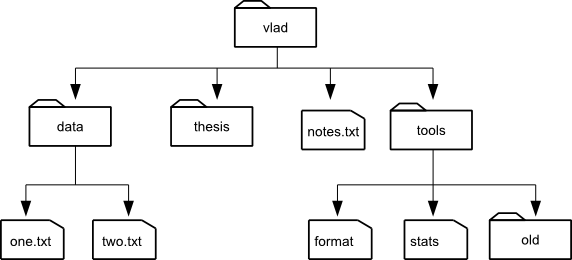
\includegraphics{novice/shell/img/find-file-tree.png}

Vlad's home directory contains one file called \texttt{notes.txt} and
four subdirectories: \texttt{thesis} (which is sadly empty),
\texttt{data} (which contains two files \texttt{one.txt} and
\texttt{two.txt}), a \texttt{tools} directory that contains the programs
\texttt{format} and \texttt{stats}, and an empty subdirectory called
\texttt{old}.

For our first command, let's run \texttt{find . -type d -print}. As
always, the \texttt{.} on its own means the current working directory,
which is where we want our search to start; \texttt{-type d} means
``things that are directories'', and (unsurprisingly) \texttt{-print}
means ``print what's found''. Sure enough, \texttt{find}'s output is the
names of the five directories in our little tree (including \texttt{.}):

\begin{verbatim}
$ find . -type d -print
\end{verbatim}

\begin{verbatim}
./
./data
./thesis
./tools
./tools/old
\end{verbatim}

If we change \texttt{-type d} to \texttt{-type f}, we get a listing of
all the files instead:

\begin{verbatim}
$ find . -type f -print
\end{verbatim}

\begin{verbatim}
./data/one.txt
./data/two.txt
./notes.txt
./tools/format
./tools/stats
\end{verbatim}

\texttt{find} automatically goes into subdirectories, their
subdirectories, and so on to find everything that matches the pattern
we've given it. If we don't want it to, we can use \texttt{-maxdepth} to
restrict the depth of search:

\begin{verbatim}
$ find . -maxdepth 1 -type f -print
\end{verbatim}

\begin{verbatim}
./notes.txt
\end{verbatim}

The opposite of \texttt{-maxdepth} is \texttt{-mindepth}, which tells
\texttt{find} to only report things that are at or below a certain
depth. \texttt{-mindepth 2} therefore finds all the files that are two
or more levels below us:

\begin{verbatim}
$ find . -mindepth 2 -type f -print
\end{verbatim}

\begin{verbatim}
./data/one.txt
./data/two.txt
./tools/format
./tools/stats
\end{verbatim}

Another option is \texttt{-empty}, which restricts matches to empty
files and directories:

\begin{verbatim}
$ find . -empty -print
\end{verbatim}

\begin{verbatim}
./thesis
./tools/old
\end{verbatim}

Now let's try matching by name:

\begin{verbatim}
$ find . -name *.txt -print
\end{verbatim}

\begin{verbatim}
./notes.txt
\end{verbatim}

We expected it to find all the text files, but it only prints out
\texttt{./notes.txt}. The problem is that the shell expands wildcard
characters like \texttt{*} \emph{before} commands run. Since
\texttt{*.txt} in the current directory expands to \texttt{notes.txt},
the command we actually ran was:

\begin{verbatim}
$ find . -name notes.txt -print
\end{verbatim}

\texttt{find} did what we asked; we just asked for the wrong thing.

To get what we want, let's do what we did with \texttt{grep}: put
\texttt{*.txt} in single quotes to prevent the shell from expanding the
\texttt{*} wildcard. This way, \texttt{find} actually gets the pattern
\texttt{*.txt}, not the expanded filename \texttt{notes.txt}:

\begin{verbatim}
$ find . -name '*.txt' -print
\end{verbatim}

\begin{verbatim}
./data/one.txt
./data/two.txt
./notes.txt
\end{verbatim}

\begin{swcbox}{Listing vs. Finding}

\texttt{ls} and \texttt{find} can be made to do similar things given the
right options, but under normal circumstances, \texttt{ls} lists
everything it can, while \texttt{find} searches for things with certain
properties and shows them.

\end{swcbox}

As we said earlier, the command line's power lies in combining tools.
We've seen how to do that with pipes; let's look at another technique.
As we just saw, \texttt{find . -name '*.txt' -print} gives us a list of
all text files in or below the current directory. How can we combine
that with \texttt{wc -l} to count the lines in all those files?

The simplest way is to put the \texttt{find} command inside
\texttt{\$()}:

\begin{verbatim}
$ wc -l $(find . -name '*.txt' -print)
\end{verbatim}

\begin{verbatim}
70  ./data/one.txt
420  ./data/two.txt
30  ./notes.txt
520  total
\end{verbatim}

When the shell executes this command, the first thing it does is run
whatever is inside the \texttt{\$()}. It then replaces the \texttt{\$()}
expression with that command's output. Since the output of \texttt{find}
is the three filenames \texttt{./data/one.txt}, \texttt{./data/two.txt},
and \texttt{./notes.txt}, the shell constructs the command:

\begin{verbatim}
$ wc -l ./data/one.txt ./data/two.txt ./notes.txt
\end{verbatim}

which is what we wanted. This expansion is exactly what the shell does
when it expands wildcards like \texttt{*} and \texttt{?}, but lets us
use any command we want as our own ``wildcard''.

It's very common to use \texttt{find} and \texttt{grep} together. The
first finds files that match a pattern; the second looks for lines
inside those files that match another pattern. Here, for example, we can
find PDB files that contain iron atoms by looking for the string ``FE''
in all the \texttt{.pdb} files below the current directory:

\begin{verbatim}
$ grep FE $(find . -name '*.pdb' -print)
\end{verbatim}

\begin{verbatim}
./human/heme.pdb:ATOM  25  FE  1  -0.924  0.535  -0.518
\end{verbatim}

\begin{swcbox}{Binary Files}

We have focused exclusively on finding things in text files. What if
your data is stored as images, in databases, or in some other format?
One option would be to extend tools like \texttt{grep} to handle those
formats. This hasn't happened, and probably won't, because there are too
many formats to support.

The second option is to convert the data to text, or extract the
text-ish bits from the data. This is probably the most common approach,
since it only requires people to build one tool per data format (to
extract information). On the one hand, it makes simple things easy to
do. On the negative side, complex things are usually impossible. For
example, it's easy enough to write a program that will extract X and Y
dimensions from image files for \texttt{grep} to play with, but how
would you write something to find values in a spreadsheet whose cells
contained formulas?

The third choice is to recognize that the shell and text processing have
their limits, and to use a programming language such as Python instead.
When the time comes to do this, don't be too hard on the shell: many
modern programming languages, Python included, have borrowed a lot of
ideas from it, and imitation is also the sincerest form of praise.

\end{swcbox}

\mbox{}\paragraph{Conclusion}

The Unix shell is older than most of the people who use it. It has
survived so long because it is one of the most productive programming
environments ever created---maybe even \emph{the} most productive. Its
syntax may be cryptic, but people who have mastered it can experiment
with different commands interactively, then use what they have learned
to automate their work. Graphical user interfaces may be better at the
first, but the shell is still unbeaten at the second. And as Alfred
North Whitehead wrote in 1911, ``Civilization advances by extending the
number of important operations which we can perform without thinking
about them.''

\begin{keypoints}
\begin{swcitemize}
\item
  Use \texttt{find} to find files and directories, and \texttt{grep} to
  find text patterns in files.
\item
  \texttt{\$(command)} inserts a command's output in place.
\item
  \texttt{man command} displays the manual page for a given command.
\end{swcitemize}
\end{keypoints}

\begin{challenge}
  Write a short explanatory comment for the following shell script:

\begin{verbatim}
find . -name '*.dat' -print | wc -l | sort -n
\end{verbatim}
\end{challenge}

\begin{challenge}
  The \texttt{-v} flag to \texttt{grep} inverts pattern matching, so
  that only lines which do \emph{not} match the pattern are printed.
  Given that, which of the following commands will find all files in
  \texttt{/data} whose names end in \texttt{ose.dat} (e.g.,
  \texttt{sucrose.dat} or \texttt{maltose.dat}), but do \emph{not}
  contain the word \texttt{temp}?

  \begin{swcenumerate}
  \item
    \texttt{find /data -name '*.dat' -print \textbar{} grep ose \textbar{} grep -v temp}
  \item
    \texttt{find /data -name ose.dat -print \textbar{} grep -v temp}
  \item
    \texttt{grep -v temp \$(find /data -name '*ose.dat' -print)}
  \item
    None of the above.
  \end{swcenumerate}
\end{challenge}

\chapter{Version Control with Git}\label{s:git}

Version control is the lab notebook of the digital world: it's what
professionals use to keep track of what they've done and to collaborate
with other people. Every large software development project relies on
it, and most programmers use it for their small jobs as well. And it
isn't just for software: books (like this one), papers, small data sets,
and anything that changes over time or needs to be shared can and should
be stored in a version control system.

\section{Introducing Version Control}

Wolfman and Dracula have been hired by Universal Missions (a space
services spinoff from Euphoric State University) to figure out where the
company should send its next planetary lander. They want to be able to
work on the plans at the same time, but they have run into problems
doing this in the past. If they take turns, each one will spend a lot of
time waiting for the other to finish, but if they work on their own
copies and email changes back and forth things will be lost,
overwritten, or duplicated.

The right solution is to use \gl{version
control}{g:version-control} to manage their work. Version control is better than mailing
files back and forth because:

\begin{swcitemize}
\item
  Nothing that is committed to version control is ever lost. This means
  it can be used like the ``undo'' feature in an editor, and since all
  old versions of files are saved it's always possible to go back in
  time to see exactly who wrote what on a particular day, or what
  version of a program was used to generate a particular set of results.
\item
  It keeps a record of who made what changes when, so that if people
  have questions later on, they know who to ask.
\item
  It's hard (but not impossible) to accidentally overlook or overwrite
  someone's changes: the version control system automatically notifies
  users whenever there's a conflict between one person's work and
  another's.
\end{swcitemize}

This lesson shows how to use a popular open source version control
system called Git. It is more complex than some alternatives, but it is
widely used, both because it's easy to set up and because of a hosting
site called \urlfoot{http://github.com}{GitHub}. No matter which version
control system you use, the most important thing to learn is not the
details of their more obscure commands, but the workflow that they
encourage.

\section{A Better Kind of Backup}

\begin{objectives}
\begin{swcitemize}
\item
  Explain which initialization and configuration steps are required once
  per machine, and which are required once per repository.
\item
  Go through the modify-add-commit cycle for single and multiple files
  and explain where information is stored at each stage.
\item
  Identify and Use Git revision numbers.
\item
  Compare files with old versions of themselves.
\item
  Restore old versions of files.
\item
  Configure Git to ignore specific files, and explain why it is
  sometimes useful to do so.
\end{swcitemize}
\end{objectives}

We'll start by exploring how version control can be used to keep track
of what one person did and when. Even if you aren't collaborating with
other people, version control is much better for this than this:

\urlfoot{http://www.phdcomics.com}{
\includegraphics{novice/git/img/phd101212s.png}}

``Piled Higher and Deeper'' by Jorge Cham, http://www.phdcomics.com

\mbox{}\paragraph{Setting Up}

The first time we use Git on a new machine, we need to configure a few
things. Here's how Dracula sets up his new laptop:

\begin{verbatim}
$ git config --global user.name "Vlad Dracula"
$ git config --global user.email "vlad@tran.sylvan.ia"
$ git config --global color.ui "auto"
$ git config --global core.editor "nano"
\end{verbatim}

(Please use your own name and email address instead of Dracula's, and
please make sure you choose an editor that's actually on your system,
such as \texttt{notepad} on Windows.)

Git commands are written \texttt{git verb}, where \texttt{verb} is what
we actually want it to do. In this case, we're telling Git:

\begin{swcitemize}
\item
  our name and email address,
\item
  to colorize output,
\item
  what our favorite text editor is, and
\item
  that we want to use these settings globally (i.e., for every project),
\end{swcitemize}

The four commands above only need to be run once: the flag
\texttt{-{}-global} tells Git to use the settings for every project on
this machine.

\mbox{}\paragraph{Creating a Repository}

Once Git is configured, we can start using it. Let's create a directory
for our work:

\begin{verbatim}
$ mkdir planets
$ cd planets
\end{verbatim}

and tell Git to make it a \gl{repository}{g:repository}---a place
where Git can store old versions of our files:

\begin{verbatim}
$ git init
\end{verbatim}

If we use \texttt{ls} to show the directory's contents, it appears that
nothing has changed:

\begin{verbatim}
$ ls
\end{verbatim}

But if we add the \texttt{-a} flag to show everything, we can see that
Git has created a hidden directory called \texttt{.git}:

\begin{verbatim}
$ ls -a
\end{verbatim}

\begin{verbatim}
.  ..  .git
\end{verbatim}

Git stores information about the project in this special sub-directory.
If we ever delete it, we will lose the project's history.

We can check that everything is set up correctly by asking Git to tell
us the status of our project:

\begin{verbatim}
$ git status
\end{verbatim}

\begin{verbatim}
# On branch master
#
# Initial commit
#
nothing to commit (create/copy files and use "git add" to track)
\end{verbatim}

\mbox{}\paragraph{Tracking Changes to Files}

Let's create a file called \texttt{mars.txt} that contains some notes
about the Red Planet's suitability as a base. (We'll use \texttt{nano}
to edit the file; you can use whatever editor you like. In particular,
this does not have to be the core.editor you set globally earlier.)

\begin{verbatim}
$ nano mars.txt
\end{verbatim}

Type the text below into the \texttt{mars.txt} file:

\begin{verbatim}
Cold and dry, but everything is my favorite color
\end{verbatim}

\texttt{mars.txt} now contains a single line:

\begin{verbatim}
$ ls
\end{verbatim}

\begin{verbatim}
mars.txt
\end{verbatim}

\begin{verbatim}
$ cat mars.txt
\end{verbatim}

\begin{verbatim}
Cold and dry, but everything is my favorite color
\end{verbatim}

If we check the status of our project again, Git tells us that it's
noticed the new file:

\begin{verbatim}
$ git status
\end{verbatim}

\begin{verbatim}
# On branch master
#
# Initial commit
#
# Untracked files:
#   (use "git add <file>..." to include in what will be committed)
#
#   mars.txt
nothing added to commit but untracked files present (use "git add" to track)
\end{verbatim}

The ``untracked files'' message means that there's a file in the
directory that Git isn't keeping track of. We can tell Git that it
should do so using \texttt{git add}:

\begin{verbatim}
$ git add mars.txt
\end{verbatim}

and then check that the right thing happened:

\begin{verbatim}
$ git status
\end{verbatim}

\begin{verbatim}
# On branch master
#
# Initial commit
#
# Changes to be committed:
#   (use "git rm --cached <file>..." to unstage)
#
#   new file:   mars.txt
#
\end{verbatim}

Git now knows that it's supposed to keep track of \texttt{mars.txt}, but
it hasn't yet recorded any changes for posterity as a commit. To get it
to do that, we need to run one more command:

\begin{verbatim}
$ git commit -m "Starting to think about Mars"
\end{verbatim}

\begin{verbatim}
[master (root-commit) f22b25e] Starting to think about Mars
 1 file changed, 1 insertion(+)
 create mode 100644 mars.txt
\end{verbatim}

When we run \texttt{git commit}, Git takes everything we have told it to
save by using \texttt{git add} and stores a copy permanently inside the
special \texttt{.git} directory. This permanent copy is called a
\gl{revision}{g:revision} and its short identifier is
\texttt{f22b25e}. (Your revision may have another identifier.)

We use the \texttt{-m} flag (for ``message'') to record a comment that
will help us remember later on what we did and why. If we just run
\texttt{git commit} without the \texttt{-m} option, Git will launch
\texttt{nano} (or whatever other editor we configured at the start) so
that we can write a longer message.

If we run \texttt{git status} now:

\begin{verbatim}
$ git status
\end{verbatim}

\begin{verbatim}
# On branch master
nothing to commit, working directory clean
\end{verbatim}

it tells us everything is up to date. If we want to know what we've done
recently, we can ask Git to show us the project's history using
\texttt{git log}:

\begin{verbatim}
$ git log
\end{verbatim}

\begin{verbatim}
commit f22b25e3233b4645dabd0d81e651fe074bd8e73b
Author: Vlad Dracula <vlad@tran.sylvan.ia>
Date:   Thu Aug 22 09:51:46 2013 -0400

    Starting to think about Mars
\end{verbatim}

\texttt{git log} lists all revisions made to a repository in reverse
chronological order. The listing for each revision includes the
revision's full identifier (which starts with the same characters as the
short identifier printed by the \texttt{git commit} command earlier),
the revision's author, when it was created, and the log message Git was
given when the revision was created.

\begin{swcbox}{Where Are My Changes?}

If we run \texttt{ls} at this point, we will still see just one file
called \texttt{mars.txt}. That's because Git saves information about
files' history in the special \texttt{.git} directory mentioned earlier
so that our filesystem doesn't become cluttered (and so that we can't
accidentally edit or delete an old version).

\end{swcbox}

\mbox{}\paragraph{Changing a File}

Now suppose Dracula adds more information to the file. (Again, we'll
edit with \texttt{nano} and then \texttt{cat} the file to show its
contents; you may use a different editor, and don't need to
\texttt{cat}.)

\begin{verbatim}
$ nano mars.txt
$ cat mars.txt
\end{verbatim}

\begin{verbatim}
Cold and dry, but everything is my favorite color
The two moons may be a problem for Wolfman
\end{verbatim}

When we run \texttt{git status} now, it tells us that a file it already
knows about has been modified:

\begin{verbatim}
$ git status
\end{verbatim}

\begin{verbatim}
# On branch master
# Changes not staged for commit:
#   (use "git add <file>..." to update what will be committed)
#   (use "git checkout -- <file>..." to discard changes in working directory)
#
#   modified:   mars.txt
#
no changes added to commit (use "git add" and/or "git commit -a")
\end{verbatim}

The last line is the key phrase: ``no changes added to commit''. We have
changed this file, but we haven't told Git we will want to save those
changes (which we do with \texttt{git add}) much less actually saved
them. Let's double-check our work using \texttt{git diff}, which shows
us the differences between the current state of the file and the most
recently saved version:

\begin{verbatim}
$ git diff
\end{verbatim}

\begin{verbatim}
diff --git a/mars.txt b/mars.txt
index df0654a..315bf3a 100644
--- a/mars.txt
+++ b/mars.txt
@@ -1 +1,2 @@
 Cold and dry, but everything is my favorite color
+The two moons may be a problem for Wolfman
\end{verbatim}

The output is cryptic because it is actually a series of commands for
tools like editors and \texttt{patch} telling them how to reconstruct
one file given the other. If we can break it down into pieces:

\begin{swcenumerate}
\item
  The first line tells us that Git is using the Unix \texttt{diff}
  command to compare the old and new versions of the file.
\item
  The second line tells exactly which \gl{revisions}{g:revision}
  of the file Git is comparing; \texttt{df0654a} and \texttt{315bf3a}
  are unique computer-generated labels for those revisions.
\item
  The remaining lines show us the actual differences and the lines on
  which they occur. In particular, the \texttt{+} markers in the first
  column show where we are adding lines.
\end{swcenumerate}

Let's commit our change:

\begin{verbatim}
$ git commit -m "Concerns about Mars's moons on my furry friend"
\end{verbatim}

\begin{verbatim}
# On branch master
# Changes not staged for commit:
#   (use "git add <file>..." to update what will be committed)
#   (use "git checkout -- <file>..." to discard changes in working directory)
#
#   modified:   mars.txt
#
no changes added to commit (use "git add" and/or "git commit -a")
\end{verbatim}

Whoops: Git won't commit because we didn't use \texttt{git add} first.
Let's fix that:

\begin{verbatim}
$ git add mars.txt
$ git commit -m "Concerns about Mars's moons on my furry friend"
\end{verbatim}

\begin{verbatim}
[master 34961b1] Concerns about Mars's moons on my furry friend
 1 file changed, 1 insertion(+)
\end{verbatim}

Git insists that we add files to the set we want to commit before
actually committing anything because we may not want to commit
everything at once. For example, suppose we're adding a few citations to
our supervisor's work to our thesis. We might want to commit those
additions, and the corresponding addition to the bibliography, but
\emph{not} commit the work we're doing on the conclusion (which we
haven't finished yet).

To allow for this, Git has a special staging area where it keeps track
of things that have been added to the current
\gl{change set}{g:change-set} but not yet committed.
\texttt{git add} puts things in this area, and \texttt{git commit} then
copies them to long-term storage (as a commit):

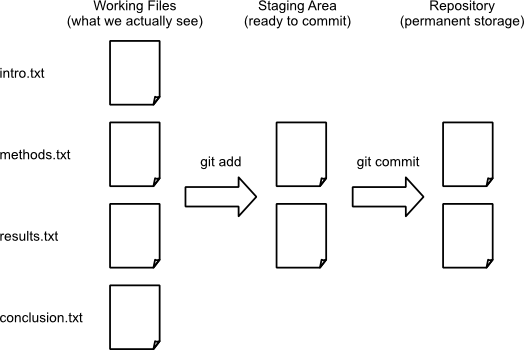
\includegraphics{novice/git/img/git-staging-area.png}

Let's watch as our changes to a file move from our editor to the staging
area and into long-term storage. First, we'll add another line to the
file:

\begin{verbatim}
$ nano mars.txt
$ cat mars.txt
\end{verbatim}

\begin{verbatim}
Cold and dry, but everything is my favorite color
The two moons may be a problem for Wolfman
But the Mummy will appreciate the lack of humidity
\end{verbatim}

\begin{verbatim}
$ git diff
\end{verbatim}

\begin{verbatim}
diff --git a/mars.txt b/mars.txt
index 315bf3a..b36abfd 100644
--- a/mars.txt
+++ b/mars.txt
@@ -1,2 +1,3 @@
 Cold and dry, but everything is my favorite color
 The two moons may be a problem for Wolfman
+But the Mummy will appreciate the lack of humidity
\end{verbatim}

So far, so good: we've added one line to the end of the file (shown with
a \texttt{+} in the first column). Now let's put that change in the
staging area and see what \texttt{git diff} reports:

\begin{verbatim}
$ git add mars.txt
$ git diff
\end{verbatim}

There is no output: as far as Git can tell, there's no difference
between what it's been asked to save permanently and what's currently in
the directory. However, if we do this:

\begin{verbatim}
$ git diff --staged
\end{verbatim}

\begin{verbatim}
diff --git a/mars.txt b/mars.txt
index 315bf3a..b36abfd 100644
--- a/mars.txt
+++ b/mars.txt
@@ -1,2 +1,3 @@
 Cold and dry, but everything is my favorite color
 The two moons may be a problem for Wolfman
+But the Mummy will appreciate the lack of humidity
\end{verbatim}

it shows us the difference between the last committed change and what's
in the staging area. Let's save our changes:

\begin{verbatim}
$ git commit -m "Thoughts about the climate"
\end{verbatim}

\begin{verbatim}
[master 005937f] Thoughts about the climate
 1 file changed, 1 insertion(+)
\end{verbatim}

check our status:

\begin{verbatim}
$ git status
\end{verbatim}

\begin{verbatim}
# On branch master
nothing to commit, working directory clean
\end{verbatim}

and look at the history of what we've done so far:

\begin{verbatim}
$ git log
\end{verbatim}

\begin{verbatim}
commit 005937fbe2a98fb83f0ade869025dc2636b4dad5
Author: Vlad Dracula <vlad@tran.sylvan.ia>
Date:   Thu Aug 22 10:14:07 2013 -0400

    Thoughts about the climate

commit 34961b159c27df3b475cfe4415d94a6d1fcd064d
Author: Vlad Dracula <vlad@tran.sylvan.ia>
Date:   Thu Aug 22 10:07:21 2013 -0400

    Concerns about Mars's moons on my furry friend

commit f22b25e3233b4645dabd0d81e651fe074bd8e73b
Author: Vlad Dracula <vlad@tran.sylvan.ia>
Date:   Thu Aug 22 09:51:46 2013 -0400

    Starting to think about Mars
\end{verbatim}

\mbox{}\paragraph{Exploring History}

If we want to see what we changed when, we use \texttt{git diff} again,
but refer to old versions using the notation
\texttt{HEAD\textasciitilde{}1}, \texttt{HEAD\textasciitilde{}2}, and so
on:

\begin{verbatim}
$ git diff HEAD~1 mars.txt
\end{verbatim}

\begin{verbatim}
diff --git a/mars.txt b/mars.txt
index 315bf3a..b36abfd 100644
--- a/mars.txt
+++ b/mars.txt
@@ -1,2 +1,3 @@
 Cold and dry, but everything is my favorite color
 The two moons may be a problem for Wolfman
+But the Mummy will appreciate the lack of humidity
\end{verbatim}

\begin{verbatim}
$ git diff HEAD~2 mars.txt
\end{verbatim}

\begin{verbatim}
diff --git a/mars.txt b/mars.txt
index df0654a..b36abfd 100644
--- a/mars.txt
+++ b/mars.txt
@@ -1 +1,3 @@
 Cold and dry, but everything is my favorite color
+The two moons may be a problem for Wolfman
+But the Mummy will appreciate the lack of humidity
\end{verbatim}

In this way, we build up a chain of revisions. The most recent end of
the chain is referred to as \texttt{HEAD}; we can refer to previous
revisions using the \texttt{\textasciitilde{}} notation, so
\texttt{HEAD\textasciitilde{}1} (pronounced ``head minus one'') means
``the previous revision'', while \texttt{HEAD\textasciitilde{}123} goes
back 123 revisions from where we are now.

We can also refer to revisions using those long strings of digits and
letters that \texttt{git log} displays. These are unique IDs for the
changes, and ``unique'' really does mean unique: every change to any set
of files on any machine has a unique 40-character identifier. Our first
commit was given the ID f22b25e3233b4645dabd0d81e651fe074bd8e73b, so
let's try this:

\begin{verbatim}
$ git diff f22b25e3233b4645dabd0d81e651fe074bd8e73b mars.txt
\end{verbatim}

\begin{verbatim}
diff --git a/mars.txt b/mars.txt
index df0654a..b36abfd 100644
--- a/mars.txt
+++ b/mars.txt
@@ -1 +1,3 @@
 Cold and dry, but everything is my favorite color
+The two moons may be a problem for Wolfman
+But the Mummy will appreciate the lack of humidity
\end{verbatim}

That's the right answer, but typing random 40-character strings is
annoying, so Git lets us use just the first few:

\begin{verbatim}
$ git diff f22b25e mars.txt
\end{verbatim}

\begin{verbatim}
diff --git a/mars.txt b/mars.txt
index df0654a..b36abfd 100644
--- a/mars.txt
+++ b/mars.txt
@@ -1 +1,3 @@
 Cold and dry, but everything is my favorite color
+The two moons may be a problem for Wolfman
+But the Mummy will appreciate the lack of humidity
\end{verbatim}

\mbox{}\paragraph{Recovering Old Versions}

All right: we can save changes to files and see what we've changed---how
can we restore older versions of things? Let's suppose we accidentally
overwrite our file:

\begin{verbatim}
$ nano mars.txt
$ cat mars.txt
\end{verbatim}

\begin{verbatim}
We will need to manufacture our own oxygen
\end{verbatim}

\texttt{git status} now tells us that the file has been changed, but
those changes haven't been staged:

\begin{verbatim}
$ git status
\end{verbatim}

\begin{verbatim}
# On branch master
# Changes not staged for commit:
#   (use "git add <file>..." to update what will be committed)
#   (use "git checkout -- <file>..." to discard changes in working directory)
#
#   modified:   mars.txt
#
no changes added to commit (use "git add" and/or "git commit -a")
\end{verbatim}

We can put things back the way they were by using \texttt{git checkout}:

\begin{verbatim}
$ git checkout HEAD mars.txt
$ cat mars.txt
\end{verbatim}

\begin{verbatim}
Cold and dry, but everything is my favorite color
The two moons may be a problem for Wolfman
But the Mummy will appreciate the lack of humidity
\end{verbatim}

As you might guess from its name, \texttt{git checkout} checks out
(i.e., restores) an old version of a file. In this case, we're telling
Git that we want to recover the version of the file recorded in
\texttt{HEAD}, which is the last saved revision. If we want to go back
even further, we can use a revision identifier instead:

\begin{verbatim}
$ git checkout f22b25e mars.txt
\end{verbatim}

It's important to remember that we must use the revision number that
identifies the state of the repository \emph{before} the change we're
trying to undo. A common mistake is to use the revision number of the
commit in which we made the change we're trying to get rid of:

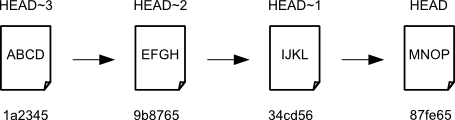
\includegraphics{novice/git/img/git-when-revisions-updated.png}

\begin{swcbox}{Simplifying the Common Case}

If you read the output of \texttt{git status} carefully, you'll see that
it includes this hint:

\begin{verbatim}
(use "git checkout -- <file>..." to discard changes in working directory)
\end{verbatim}

As it says, \texttt{git checkout} without a version identifier restores
files to the state saved in \texttt{HEAD}. The double dash \texttt{-{}-}
is needed to separate the names of the files being recovered from the
command itself: without it, Git would try to use the name of the file as
the revision identifier.

\end{swcbox}

The fact that files can be reverted one by one tends to change the way
people organize their work. If everything is in one large document, it's
hard (but not impossible) to undo changes to the introduction without
also undoing changes made later to the conclusion. If the introduction
and conclusion are stored in separate files, on the other hand, moving
backward and forward in time becomes much easier.

\mbox{}\paragraph{Ignoring Things}

What if we have files that we do not want Git to track for us, like
backup files created by our editor or intermediate files created during
data analysis. Let's create a few dummy files:

\begin{verbatim}
$ mkdir results
$ touch a.dat b.dat c.dat results/a.out results/b.out
\end{verbatim}

and see what Git says:

\begin{verbatim}
$ git status
\end{verbatim}

\begin{verbatim}
# On branch master
# Untracked files:
#   (use "git add <file>..." to include in what will be committed)
#
#   a.dat
#   b.dat
#   c.dat
#   results/
nothing added to commit but untracked files present (use "git add" to track)
\end{verbatim}

Putting these files under version control would be a waste of disk
space. What's worse, having them all listed could distract us from
changes that actually matter, so let's tell Git to ignore them.

We do this by creating a file in the root directory of our project
called \texttt{.gitignore}.

\begin{verbatim}
$ nano .gitignore
$ cat .gitignore
\end{verbatim}

\begin{verbatim}
*.dat
results/
\end{verbatim}

These patterns tell Git to ignore any file whose name ends in
\texttt{.dat} and everything in the \texttt{results} directory. (If any
of these files were already being tracked, Git would continue to track
them.)

Once we have created this file, the output of \texttt{git status} is
much cleaner:

\begin{verbatim}
$ git status
\end{verbatim}

\begin{verbatim}
# On branch master
# Untracked files:
#   (use "git add <file>..." to include in what will be committed)
#
#   .gitignore
nothing added to commit but untracked files present (use "git add" to track)
\end{verbatim}

The only thing Git notices now is the newly-created \texttt{.gitignore}
file. You might think we wouldn't want to track it, but everyone we're
sharing our repository with will probably want to ignore the same things
that we're ignoring. Let's add and commit \texttt{.gitignore}:

\begin{verbatim}
$ git add .gitignore
$ git commit -m "Add the ignore file"
$ git status
\end{verbatim}

\begin{verbatim}
# On branch master
nothing to commit, working directory clean
\end{verbatim}

As a bonus, using \texttt{.gitignore} helps us avoid accidentally adding
files to the repository that we don't want.

\begin{verbatim}
$ git add a.dat
\end{verbatim}

\begin{verbatim}
The following paths are ignored by one of your .gitignore files:
a.dat
Use -f if you really want to add them.
fatal: no files added
\end{verbatim}

If we really want to override our ignore settings, we can use
\texttt{git add -f} to force Git to add something. We can also always
see the status of ignored files if we want:

\begin{verbatim}
$ git status --ignored
\end{verbatim}

\begin{verbatim}
# On branch master
# Ignored files:
#  (use "git add -f <file>..." to include in what will be committed)
#
#        a.dat
#        b.dat
#        c.dat
#        results/

nothing to commit, working directory clean
\end{verbatim}

\begin{keypoints}
\begin{swcitemize}
\item
  Use \texttt{git config} to configure a user name, email address,
  editor, and other preferences once per machine.
\item
  \texttt{git init} initializes a repository.
\item
  \texttt{git status} shows the status of a repository.
\item
  Files can be stored in a project's working directory (which users
  see), the staging area (where the next commit is being built up) and
  the local repository (where snapshots are permanently recorded).
\item
  \texttt{git add} puts files in the staging area.
\item
  \texttt{git commit} creates a snapshot of the staging area in the
  local repository.
\item
  Always write a log message when committing changes.
\item
  \texttt{git diff} displays differences between revisions.
\item
  \texttt{git checkout} recovers old versions of files.
\item
  The \texttt{.gitignore} file tells Git what files to ignore.
\end{swcitemize}
\end{keypoints}

\begin{challenge}
  Create a new Git repository on your computer called \texttt{bio}.
  Write a three-line biography for yourself in a file called
  \texttt{me.txt}, commit your changes, then modify one line and add a
  fourth and display the differences between its updated state and its
  original state.
\end{challenge}

\begin{challenge}
  The following sequence of commands creates one Git repository inside
  another:

\begin{verbatim}
cd           # return to home directory
mkdir alpha  # make a new directory alpha
cd alpha     # go into alpha
git init     # make the alpha directory a Git repository
mkdir beta   # make a sub-directory alpha/beta
cd beta      # go into alpha/beta
git init     # make the beta sub-directory a Git repository
\end{verbatim}

  Why is it a bad idea to do this?
\end{challenge}

\section{Collaborating}

\begin{objectives}
\begin{swcitemize}
\item
  Explain what remote repositories are and why they are useful.
\item
  Explain what happens when a remote repository is cloned.
\item
  Explain what happens when changes are pushed to or pulled from a
  remote repository.
\end{swcitemize}
\end{objectives}

Version control really comes into its own when we begin to collaborate
with other people. We already have most of the machinery we need to do
this; the only thing missing is to copy changes from one repository to
another.

Systems like Git allow us to move work between any two repositories. In
practice, though, it's easiest to use one copy as a central hub, and to
keep it on the web rather than on someone's laptop. Most programmers use
hosting services like \urlfoot{http://github.com}{GitHub} or
\urlfoot{http://bitbucket.org}{BitBucket} to hold those master copies;
we'll explore the pros and cons of this in the final section of this
lesson.

Let's start by sharing the changes we've made to our current project
with the world. Log in to GitHub, then click on the icon in the top
right corner to create a new repository called \texttt{planets}:


\includegraphics{novice/git/img/github-create-repo-01.png}

Name your repository ``planets'' and then click ``Create Repository'':

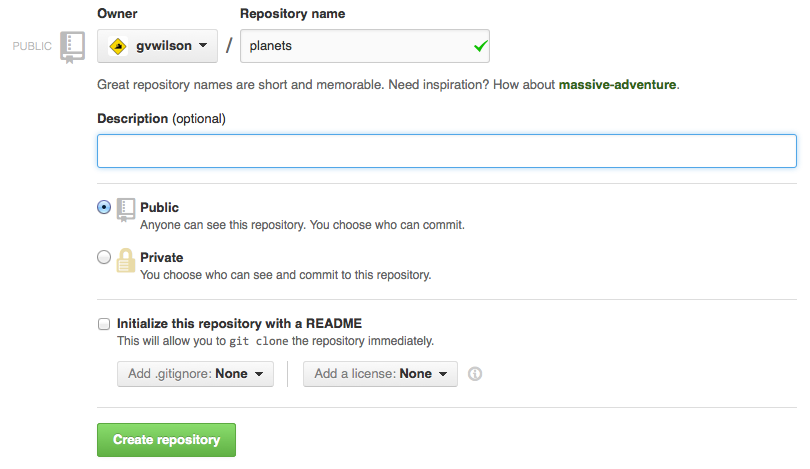
\includegraphics{novice/git/img/github-create-repo-02.png}

As soon as the repository is created, GitHub displays a page with a URL
and some information on how to configure your local repository:

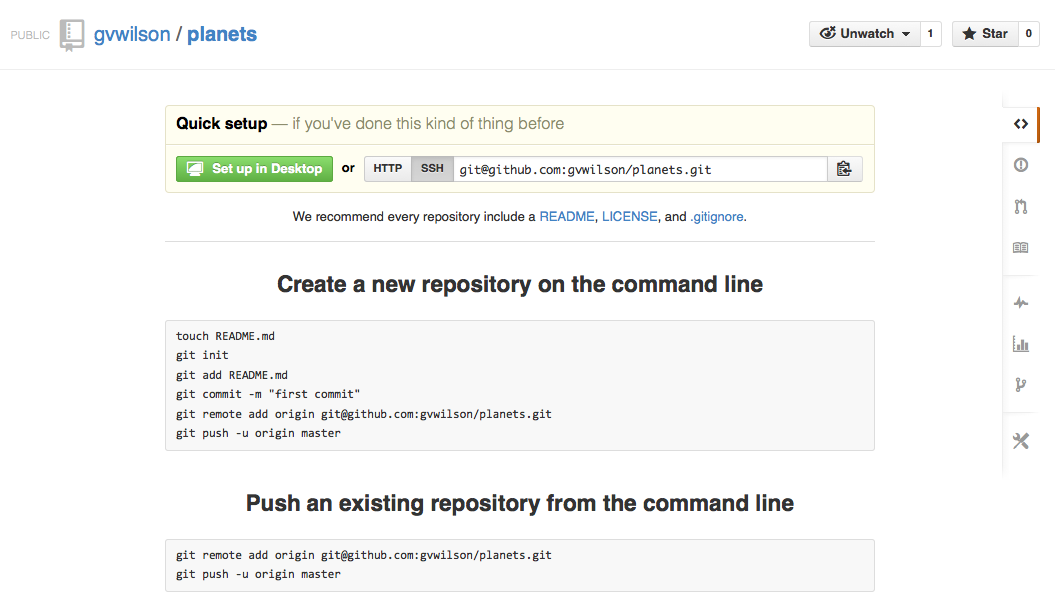
\includegraphics{novice/git/img/github-create-repo-03.png}

This effectively does the following on GitHub's servers:

\begin{verbatim}
$ mkdir planets
$ cd planets
$ git init
\end{verbatim}

Our local repository still contains our earlier work on
\texttt{mars.txt}, but the remote repository on GitHub doesn't contain
any files yet:

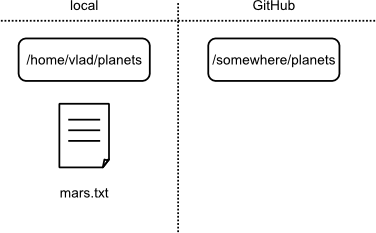
\includegraphics{novice/git/img/git-freshly-made-github-repo.png}

The next step is to connect the two repositories. We do this by making
the GitHub repository a \gl{remote}{g:repository-remote} for the
local repository. The home page of the repository on GitHub includes the
string we need to identify it:

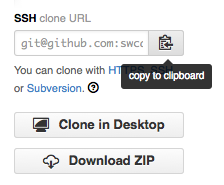
\includegraphics{novice/git/img/github-find-repo-string.png}

Click on the `HTTPS' link to change the \gl{protocol}{g:protocol}
from SSH to HTTPS. It's slightly less convenient for day-to-day use, but
much less work for beginners to set up:

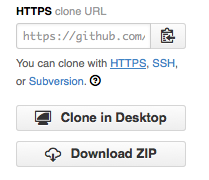
\includegraphics{novice/git/img/github-change-repo-string.png}

Copy that URL from the browser, go into the local \texttt{planets}
repository, and run this command:

\begin{verbatim}
$ git remote add origin https://github.com/vlad/planets
\end{verbatim}

Make sure to use the URL for your repository rather than Vlad's: the
only difference should be your username instead of \texttt{vlad}.

We can check that the command has worked by running
\texttt{git remote -v}:

\begin{verbatim}
$ git remote -v
\end{verbatim}

\begin{verbatim}
origin   https://github.com/vlad/planets.git (push)
origin   https://github.com/vlad/planets.git (fetch)
\end{verbatim}

The name \texttt{origin} is a local nickname for your remote repository:
we could use something else if we wanted to, but \texttt{origin} is by
far the most common choice.

Once the nickname \texttt{origin} is set up, this command will push the
changes from our local repository to the repository on GitHub:

\begin{verbatim}
$ git push origin master
\end{verbatim}

\begin{verbatim}
Counting objects: 9, done.
Delta compression using up to 4 threads.
Compressing objects: 100% (6/6), done.
Writing objects: 100% (9/9), 821 bytes, done.
Total 9 (delta 2), reused 0 (delta 0)
To https://github.com/vlad/planets
 * [new branch]      master -> master
Branch master set up to track remote branch master from origin.
\end{verbatim}

Our local and remote repositories are now in this state:

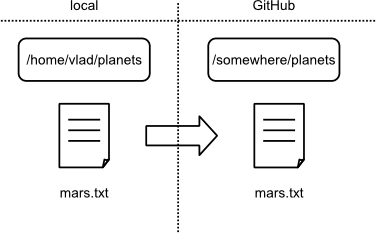
\includegraphics{novice/git/img/github-repo-after-first-push.png}

\begin{swcbox}{The `-u' Flag}

You may see a \texttt{-u} option used with \texttt{git push} in some
documentation. It is related to concepts we cover in our intermediate
lesson, and can safely be ignored for now.

\end{swcbox}

We can pull changes from the remote repository to the local one as well:

\begin{verbatim}
$ git pull origin master
\end{verbatim}

\begin{verbatim}
From https://github.com/vlad/planets
 * branch            master     -> FETCH_HEAD
Already up-to-date.
\end{verbatim}

Pulling has no effect in this case because the two repositories are
already synchronized. If someone else had pushed some changes to the
repository on GitHub, though, this command would download them to our
local repository.

We can simulate working with a collaborator using another copy of the
repository on our local machine. To do this, \texttt{cd} to the
directory \texttt{/tmp}. (Note the absolute path: don't make
\texttt{tmp} a subdirectory of the existing repository). Instead of
creating a new repository here with \texttt{git init}, we will
\gl{clone}{g:repository-clone} the existing repository from
GitHub:

\begin{verbatim}
$ cd /tmp
$ git clone https://github.com/vlad/planets.git
\end{verbatim}

\texttt{git clone} creates a fresh local copy of a remote repository.
(We did it in \texttt{/tmp} or some other directory so that we don't
overwrite our existing \texttt{planets} directory.) Our computer now has
two copies of the repository:

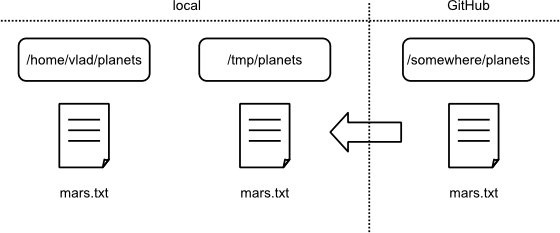
\includegraphics{novice/git/img/git-after-duplicate-clone.png}

Let's make a change in the copy in \texttt{/tmp/planets}:

\begin{verbatim}
$ cd /tmp/planets
$ nano pluto.txt
$ cat pluto.txt
\end{verbatim}

\begin{verbatim}
It is so a planet!
\end{verbatim}

\begin{verbatim}
$ git add pluto.txt
$ git commit -m "Some notes about Pluto"
\end{verbatim}

\begin{verbatim}
 1 file changed, 1 insertion(+)
 create mode 100644 pluto.txt
\end{verbatim}

then push the change to GitHub:

\begin{verbatim}
$ git push origin master
\end{verbatim}

\begin{verbatim}
Counting objects: 4, done.
Delta compression using up to 4 threads.
Compressing objects: 100% (2/2), done.
Writing objects: 100% (3/3), 306 bytes, done.
Total 3 (delta 0), reused 0 (delta 0)
To https://github.com/vlad/planets.git
   9272da5..29aba7c  master -> master
\end{verbatim}

Note that we didn't have to create a remote called \texttt{origin}: Git
does this automatically, using that name, when we clone a repository.
(This is why \texttt{origin} was a sensible choice earlier when we were
setting up remotes by hand.)

Our three repositories now look like this:

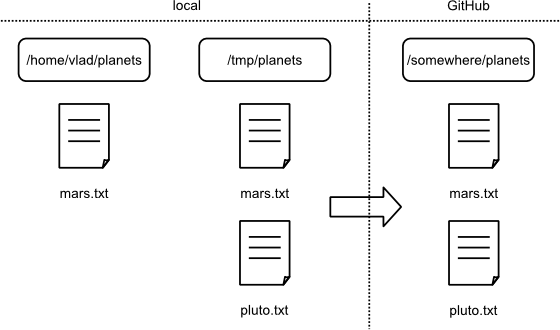
\includegraphics{novice/git/img/git-after-change-to-duplicate-repo.png}

We can now download changes into the original repository on our machine:

\begin{verbatim}
$ cd ~/planets
$ git pull origin master
\end{verbatim}

\begin{verbatim}
remote: Counting objects: 4, done.
remote: Compressing objects: 100% (2/2), done.
remote: Total 3 (delta 0), reused 3 (delta 0)
Unpacking objects: 100% (3/3), done.
From https://github.com/vlad/planets
 * branch            master     -> FETCH_HEAD
Updating 9272da5..29aba7c
Fast-forward
 pluto.txt | 1 +
 1 file changed, 1 insertion(+)
 create mode 100644 pluto.txt
\end{verbatim}

which gives us this:

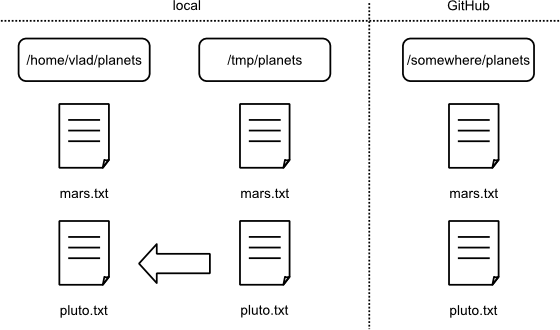
\includegraphics{novice/git/img/git-after-pulling-to-local-repo.png}

In practice, we would probably never have two copies of the same remote
repository on our laptop at once. Instead, one of those copies would be
on our laptop, and the other on a lab machine, or on someone else's
computer. Pushing and pulling changes gives us a reliable way to share
work between different people and machines.

\begin{keypoints}
\begin{swcitemize}
\item
  A local Git repository can be connected to one or more remote
  repositories.
\item
  Use the HTTPS protocol to connect to remote repositories until you
  have learned how to set up SSH.
\item
  \texttt{git push} copies changes from a local repository to a remote
  repository.
\item
  \texttt{git pull} copies changes from a remote repository to a local
  repository.
\item
  \texttt{git clone} copies a remote repository to create a local
  repository with a remote called \texttt{origin} automatically set up.
\end{swcitemize}
\end{keypoints}

\begin{challenge}
  Create a repository on GitHub, clone it, add a file, push those
  changes to GitHub, and then look at the
  \gl{timestamp}{g:timestamp} of the change on GitHub. How does
  GitHub record times, and why?
\end{challenge}

\section{Conflicts}

\begin{objectives}
\begin{swcitemize}
\item
  Explain what conflicts are and when they can occur.
\item
  Resolve conflicts resulting from a merge.
\end{swcitemize}
\end{objectives}

As soon as people can work in parallel, someone's going to step on
someone else's toes. This will even happen with a single person: if we
are working on a piece of software on both our laptop and a server in
the lab, we could make different changes to each copy. Version control
helps us manage these \gl{conflicts}{g:conflict} by giving us
tools to \gl{resolve}{g:resolve} overlapping changes.

To see how we can resolve conflicts, we must first create one. The file
\texttt{mars.txt} currently looks like this in both local copies of our
\texttt{planets} repository (the one in our home directory and the one
in \texttt{/tmp}):

\begin{verbatim}
$ cat mars.txt
\end{verbatim}

\begin{verbatim}
Cold and dry, but everything is my favorite color
The two moons may be a problem for Wolfman
But the Mummy will appreciate the lack of humidity
\end{verbatim}

Let's add a line to the copy under our home directory:

\begin{verbatim}
$ nano mars.txt
$ cat mars.txt
\end{verbatim}

\begin{verbatim}
Cold and dry, but everything is my favorite color
The two moons may be a problem for Wolfman
But the Mummy will appreciate the lack of humidity
This line added to our home copy
\end{verbatim}

and then push the change to GitHub:

\begin{verbatim}
$ git add mars.txt
$ git commit -m "Adding a line in our home copy"
\end{verbatim}

\begin{verbatim}
[master 5ae9631] Adding a line in our home copy
 1 file changed, 1 insertion(+)
\end{verbatim}

\begin{verbatim}
$ git push origin master
\end{verbatim}

\begin{verbatim}
Counting objects: 5, done.
Delta compression using up to 4 threads.
Compressing objects: 100% (3/3), done.
Writing objects: 100% (3/3), 352 bytes, done.
Total 3 (delta 1), reused 0 (delta 0)
To https://github.com/vlad/planets
   29aba7c..dabb4c8  master -> master
\end{verbatim}

Our repositories are now in this state:

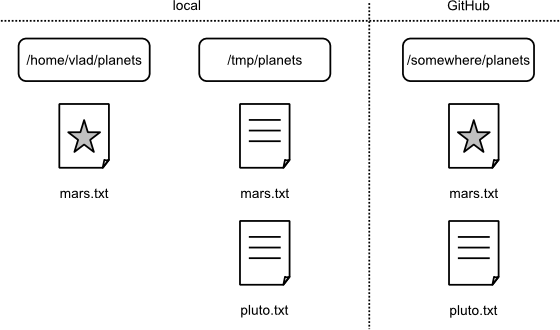
\includegraphics{novice/git/img/git-after-first-conflicting-change.png}

Now let's switch to the copy under \texttt{/tmp} and make a different
change there \emph{without} updating from GitHub:

\begin{verbatim}
$ cd /tmp/planets
$ nano mars.txt
$ cat mars.txt
\end{verbatim}

\begin{verbatim}
Cold and dry, but everything is my favorite color
The two moons may be a problem for Wolfman
But the Mummy will appreciate the lack of humidity
We added a different line in the temporary copy
\end{verbatim}

We can commit the change locally:

\begin{verbatim}
$ git add mars.txt
$ git commit -m "Adding a line in the temporary copy"
\end{verbatim}

\begin{verbatim}
[master 07ebc69] Adding a line in the temporary copy
 1 file changed, 1 insertion(+)
\end{verbatim}

but Git won't let us push it to GitHub:

\begin{verbatim}
$ git push origin master
\end{verbatim}

\begin{verbatim}
To https://github.com/vlad/planets.git
 ! [rejected]        master -> master (non-fast-forward)
error: failed to push some refs to 'https://github.com/vlad/planets.git'
hint: Updates were rejected because the tip of your current branch is behind
hint: its remote counterpart. Merge the remote changes (e.g. 'git pull')
hint: before pushing again.
hint: See the 'Note about fast-forwards' in 'git push --help' for details.
\end{verbatim}

Git detects that the changes made in one copy overlap with those made in
the other and stops us from trampling on our previous work. What we have
to do is pull the changes from GitHub,
\gl{merge}{g:repository-merge} them into the copy we're currently
working in, and then push that. Let's start by pulling:

\begin{verbatim}
$ git pull origin master
\end{verbatim}

\begin{verbatim}
remote: Counting objects: 5, done.
remote: Compressing objects: 100% (2/2), done.
remote: Total 3 (delta 1), reused 3 (delta 1)
Unpacking objects: 100% (3/3), done.
From https://github.com/vlad/planets
 * branch            master     -> FETCH_HEAD
Auto-merging mars.txt
CONFLICT (content): Merge conflict in mars.txt
Automatic merge failed; fix conflicts and then commit the result.
\end{verbatim}

\texttt{git pull} tells us there's a conflict, and marks that conflict
in the affected file:

\begin{verbatim}
$ cat mars.txt
\end{verbatim}

\begin{verbatim}
Cold and dry, but everything is my favorite color
The two moons may be a problem for Wolfman
But the Mummy will appreciate the lack of humidity
<<<<<<< HEAD
We added a different line in the temporary copy
=======
This line added to our home copy
>>>>>>> dabb4c8c450e8475aee9b14b4383acc99f42af1d
\end{verbatim}

Our change---the one in \texttt{HEAD}---is preceded by
\texttt{\textless{}\textless{}\textless{}\textless{}\textless{}\textless{}\textless{}}.
Git has then inserted \texttt{=======} as a separator between the
conflicting changes and marked the end of the content downloaded from
GitHub with
\texttt{\textgreater{}\textgreater{}\textgreater{}\textgreater{}\textgreater{}\textgreater{}\textgreater{}}.
(The string of letters and digits after that marker identifies the
revision we've just downloaded.)

It is now up to us to edit this file to remove these markers and
reconcile the changes. We can do anything we want: keep the change in
this branch, keep the change made in the other, write something new to
replace both, or get rid of the change entirely. Let's replace both so
that the file looks like this:

\begin{verbatim}
$ cat mars.txt
\end{verbatim}

\begin{verbatim}
Cold and dry, but everything is my favorite color
The two moons may be a problem for Wolfman
But the Mummy will appreciate the lack of humidity
We removed the conflict on this line
\end{verbatim}

To finish merging, we add \texttt{mars.txt} to the changes being made by
the merge and then commit:

\begin{verbatim}
$ git add mars.txt
$ git status
\end{verbatim}

\begin{verbatim}
# On branch master
# All conflicts fixed but you are still merging.
#   (use "git commit" to conclude merge)
#
# Changes to be committed:
#
#   modified:   mars.txt
#
\end{verbatim}

\begin{verbatim}
$ git commit -m "Merging changes from GitHub"
\end{verbatim}

\begin{verbatim}
[master 2abf2b1] Merging changes from GitHub
\end{verbatim}

Our repositories now look like this:

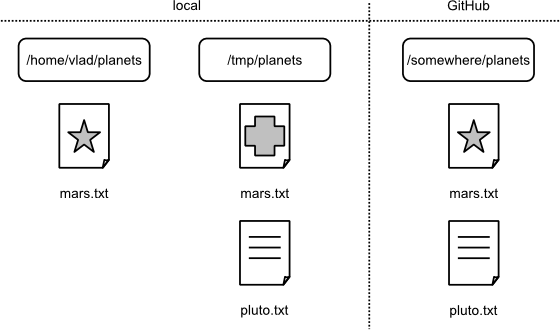
\includegraphics{novice/git/img/git-after-second-conflicting-change.png}

so we push our changes to GitHub:

\begin{verbatim}
$ git push origin master
\end{verbatim}

\begin{verbatim}
Counting objects: 10, done.
Delta compression using up to 4 threads.
Compressing objects: 100% (6/6), done.
Writing objects: 100% (6/6), 697 bytes, done.
Total 6 (delta 2), reused 0 (delta 0)
To https://github.com/vlad/planets.git
   dabb4c8..2abf2b1  master -> master
\end{verbatim}

to get this:

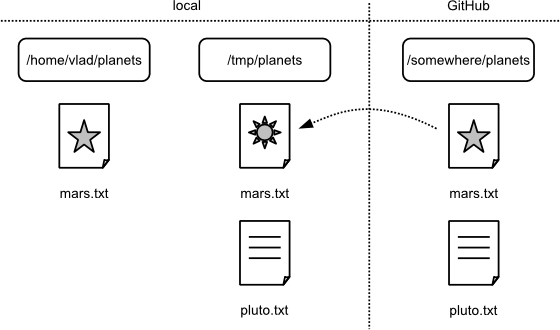
\includegraphics{novice/git/img/git-after-merging.png}

Git keeps track of what we've merged with what, so we don't have to fix
things by hand again if we switch back to the repository in our home
directory and pull from GitHub:

\begin{verbatim}
$ cd ~/planets
$ git pull origin master
\end{verbatim}

\begin{verbatim}
remote: Counting objects: 10, done.
remote: Compressing objects: 100% (4/4), done.
remote: Total 6 (delta 2), reused 6 (delta 2)
Unpacking objects: 100% (6/6), done.
From https://github.com/vlad/planets
 * branch            master     -> FETCH_HEAD
Updating dabb4c8..2abf2b1
Fast-forward
 mars.txt | 2 +-
 1 file changed, 1 insertion(+), 1 deletion(-)
\end{verbatim}

we get the merged file:

\begin{verbatim}
$ cat mars.txt
\end{verbatim}

\begin{verbatim}
Cold and dry, but everything is my favorite color
The two moons may be a problem for Wolfman
But the Mummy will appreciate the lack of humidity
We removed the conflict on this line
\end{verbatim}

We don't need to merge again because GitHub knows someone has already
done that.

Version control's ability to merge conflicting changes is another reason
users tend to divide their programs and papers into multiple files
instead of storing everything in one large file. There's another benefit
too: whenever there are repeated conflicts in a particular file, the
version control system is essentially trying to tell its users that they
ought to clarify who's responsible for what, or find a way to divide the
work up differently.

\begin{keypoints}
\begin{swcitemize}
\item
  Conflicts occur when two or more people change the same file(s) at the
  same time.
\item
  The version control system does not allow people to blindly overwrite
  each other's changes. Instead, it highlights conflicts so that they
  can be resolved.
\end{swcitemize}
\end{keypoints}

\begin{challenge}
  Clone the repository created by your instructor. Add a new file to it,
  and modify an existing file (your instructor will tell you which one).
  When asked by your instructor, pull her changes from the repository to
  create a conflict, then resolve it.
\end{challenge}

\begin{challenge}
  What does Git do when there is a conflict in an image or some other
  non-textual file that is stored in version control?
\end{challenge}

\section{Open Science}

\begin{objectives}
\begin{swcitemize}
\item
  Explain how the GNU Public License (GPL) differs from most other open
  licenses.
\item
  Explain the four kinds of restrictions that can be combined in a
  Creative Commons license.
\item
  Correctly add licensing and citation information to a project
  repository.
\item
  Outline options for hosting code and data and the pros and cons of
  each.
\end{swcitemize}
\end{objectives}

\begin{quote}
The opposite of ``open'' isn't ``closed''. The opposite of ``open'' is
``broken''. \\
--- John Wilbanks
\end{quote}

Free sharing of information might be the ideal in science, but the
reality is often more complicated. Normal practice today looks something
like this:

\begin{swcitemize}
\item
  A scientist collects some data and stores it on a machine that is
  occasionally backed up by her department.
\item
  She then writes or modifies a few small programs (which also reside on
  her machine) to analyze that data.
\item
  Once she has some results, she writes them up and submits her paper.
  She might include her data---a growing number of journals require
  this---but she probably doesn't include her code.
\item
  Time passes.
\item
  The journal sends her reviews written anonymously by a handful of
  other people in her field. She revises her paper to satisfy them,
  during which time she might also modify the scripts she wrote earlier,
  and resubmits.
\item
  More time passes.
\item
  The paper is eventually published. It might include a link to an
  online copy of her data, but the paper itself will be behind a
  paywall: only people who have personal or institutional access will be
  able to read it.
\end{swcitemize}

For a growing number of scientists, though, the process looks like this:

\begin{swcitemize}
\item
  The data that the scientist collects is stored in an open access
  repository like \urlfoot{http://figshare.com/}{figshare} or
  \urlfoot{http://datadryad.org/}{Dryad} as soon as it's collected, and
  given its own DOI.
\item
  The scientist creates a new repository on GitHub to hold her work.
\item
  As she does her analysis, she pushes changes to her scripts (and
  possibly some output files) to that repository. She also uses the
  repository for her paper; that repository is then the hub for
  collaboration with her colleagues.
\item
  When she's happy with the state of her paper, she posts a version to
  \urlfoot{http://arxiv.org/}{arXiv} or some other preprint server to
  invite feedback from peers.
\item
  Based on that feedback, she may post several revisions before finally
  submitting her paper to a journal.
\item
  The published paper includes links to her preprint and to her code and
  data repositories, which makes it much easier for other scientists to
  use her work as starting point for their own research.
\end{swcitemize}

This open model accelerates discovery: the more open work is, the more
widely it is cited and re-used. However, people who want to work this
way need to make some decisions about what exactly ``open'' means in
practice.

\mbox{}\paragraph{Licensing}

The first question is licensing. Broadly speaking, there are two kinds
of open license for software, and half a dozen for data and
publications. For software, people can choose between the
\urlfoot{http://opensource.org/licenses/GPL-3.0}{GNU Public License} (GPL)
on the one hand, and licenses like the
\urlfoot{http://opensource.org/licenses/MIT}{MIT} and
\urlfoot{http://opensource.org/licenses/BSD-2-Clause}{BSD} licenses on the
other. All of these licenses allow unrestricted sharing and modification
of programs, but the GPL is \gl{infective}{g:infective-license}:
anyone who distributes a modified version of the code (or anything that
includes GPL'd code) must make \emph{their} code freely available as
well.

Proponents of the GPL argue that this requirement is needed to ensure
that people who are benefiting from freely-available code are also
contributing back to the community. Opponents counter that many open
source projects have had long and successful lives without this
condition, and that the GPL makes it more difficult to combine code from
different sources. At the end of the day, what matters most is that:

\begin{swcenumerate}
\item
  every project have a file in its home directory called something like
  \texttt{LICENSE} or \texttt{LICENSE.txt} that clearly states what the
  license is, and
\item
  people use existing licenses rather than writing new ones.
\end{swcenumerate}

The second point is as important as the first: most scientists are not
lawyers, so wording that may seem sensible to a layperson may have
unintended gaps or consequences. The \urlfoot{http://opensource.org/}{Open
Source Initiative} maintains a list of open source licenses, and
\urlfoot{http://www.tldrlegal.com/}{tl;drLegal} explains many of them in
plain English.

When it comes to data, publications, and the like, scientists have many
more options to choose from. The good news is that an organization
called \urlfoot{http://creativecommons.org/}{Creative Commons} has prepared
a set of licenses using combinations of four basic restrictions:

\begin{swcitemize}
\item
  Attribution: derived works must give the original author credit for
  their work.
\item
  No Derivatives: people may copy the work, but must pass it along
  unchanged.
\item
  Share Alike: derivative works must license their work under the same
  terms as the original.
\item
  Noncommercial: free use is allowed, but commercial use is not.
\end{swcitemize}

These four restrictions are abbreviated ``BY'', ``ND'', ``SA'', and
``NC'' respectively, so ``CC-BY-ND'' means, ``People can re-use the work
both for free and commercially, but cannot make changes and must cite
the original.'' These \urlfoot{http://creativecommons.org/licenses/}{short
descriptions} summarize the six CC licenses in plain language, and
include links to their full legal formulations.

There is one other important license that doesn't fit into this
categorization. Scientists (and other people) can choose to put material
in the public domain, which is often abbreviated ``PD''. In this case,
anyone can do anything they want with it, without needing to cite the
original or restrict further re-use. The table below shows how the six
Creative Commons licenses and PD relate to one another:

\begin{tabular}{llllllll}
\hline\noalign{\medskip}
& Licenses that can be used for derivative work or adaptation
\\\noalign{\medskip}
Original work & by & by-nc & by-nc-nd & by-nc-sa & by-nd & by-sa & pd
\\\noalign{\medskip}
by & X & X & X & X & X & X &
\\\noalign{\medskip}
by-nc & & X & X & X & & &
\\\noalign{\medskip}
by-nc-nd & & & & & & &
\\\noalign{\medskip}
by-nc-sa & & & & X & & &
\\\noalign{\medskip}
by-nd & & & & & & &
\\\noalign{\medskip}
by-sa & & & & & & X &
\\\noalign{\medskip}
pd & X & X & X & X & X & X & X
\\\noalign{\medskip}
\hline
\end{tabular}

\urlfoot{http://software-carpentry.org/license.html}{Software Carpentry}
uses CC-BY for its lessons and the MIT License for its code in order to
encourage the widest possible re-use. Again, the most important thing is
for the \texttt{LICENSE} file in the root directory of your project to
state clearly what your license is. You may also want to include a file
called \texttt{CITATION} or \texttt{CITATION.txt} that describes how to
reference your project; the one for Software Carpentry states:

\begin{verbatim}
To reference Software Carpentry in publications, please cite both of the following:

Greg Wilson: "Software Carpentry: Lessons Learned". arXiv:1307.5448, July 2013.

@online{wilson-software-carpentry-2013,
  author      = {Greg Wilson},
  title       = {Software Carpentry: Lessons Learned},
  version     = {1},
  date        = {2013-07-20},
  eprinttype  = {arxiv},
  eprint      = {1307.5448}
}
\end{verbatim}

\mbox{}\paragraph{Hosting}

The second big question for groups that want to open up their work is
where to host their code and data. One option is for the lab, the
department, or the university to provide a server, manage accounts and
backups, and so on. The main benefit of this is that it clarifies who
owns what, which is particularly important if any of the material is
sensitive (i.e., relates to experiments involving human subjects or may
be used in a patent application). The main drawbacks are the cost of
providing the service and its longevity: a scientist who has spent ten
years collecting data would like to be sure that data will still be
available ten years from now, but that's well beyond the lifespan of
most of the grants that fund academic infrastructure.

Another option is to purchase a domain and pay an
\gl{Internet service provider}{g:isp} (ISP) to host it. This gives
the individual or group more control, and sidesteps problems that can
arise when moving from one institution to another, but requires more
time and effort to set up than either the option above or the option
below.

The third option is to use a public hosting service like
\urlfoot{http://github.com}{GitHub},
\urlfoot{http://bitbucket.org}{BitBucket},
\urlfoot{http://code.google.com}{Google Code}, or
\urlfoot{http://sourceforge.net}{SourceForge}. All of these allow people to
create repositories through a web interface, and also provide mailing
lists, ways to keep track of who's doing what, and so on. They all
benefit from economies of scale and network effects: it's easier to run
one large service well than to run many smaller services to the same
standard, and it's also easier for people to collaborate if they're
using the same service, not least because it gives them fewer passwords
to remember.

However, all of these services place some constraints on people's work.
In particular, most give users a choice: if they're willing to share
their work with others, it will be hosted for free, but if they want
privacy, they may have to pay. Sharing might seem like the only valid
choice for science, but many institutions may not allow researchers to
do this, either because they want to protect future patent applications
or simply because what's new is often also frightening.

\begin{keypoints}
\begin{swcitemize}
\item
  Open scientific work is more useful and more highly cited than closed.
\item
  People who incorporate GPL'd software into theirs must make theirs
  open; most other open licenses do not require this.
\item
  The Creative Commons family of licenses allow people to mix and match
  requirements and restrictions on attribution, creation of derivative
  works, further sharing, and commercialization.
\item
  People who are not lawyers should not try to write licenses from
  scratch.
\item
  Projects can be hosted on university servers, on personal domains, or
  on public forges.
\item
  Rules regarding intellectual property and storage of sensitive
  information apply no matter where code and data are hosted.
\end{swcitemize}
\end{keypoints}

\begin{challenge}
  Find out whether you are allowed to apply an open license to your
  software. Can you do this unilaterally, or do you need permission from
  someone in your institution? If so, who?
\end{challenge}

\begin{challenge}
  Find out whether you are allowed to host your work openly on a public
  forge. Can you do this unilaterally, or do you need permission from
  someone in your institution? If so, who?
\end{challenge}

\chapter{Programming with Python}\label{s:python}

The best way to learn how to program is to do something useful, so this
introduction to Python is built around a common scientific task: data
analysis.

Our real goal isn't to teach you Python, but to teach you the basic
concepts that all programming depends on. We use Python in our lessons
because:

\begin{swcenumerate}
\item
  we have to use \emph{something} for examples;
\item
  it's free, well-documented, and runs almost everywhere;
\item
  it has a large (and growing) user base among scientists; and
\item
  experience shows that it's easier for novices to pick up than most
  other languages.
\end{swcenumerate}

But the two most important things are to use whatever language your
colleagues are using, so that you can share you work with them easily,
and to use that language \emph{well}.

\section{Analyzing Patient Data}

We are studying inflammation in patients who have been given a new
treatment for arthritis, and need to analyze the first dozen data sets.
The data sets are stored in \gl{comma-separated values}{g:csv}
(CSV) format: each row holds information for a single patient, and the
columns represent successive days. The first few rows of our first file
look like this:

\begin{verbatim}
0,0,1,3,1,2,4,7,8,3,3,3,10,5,7,4,7,7,12,18,6,13,11,11,7,7,4,6,8,8,4,4,5,7,3,4,2,3,0,0
0,1,2,1,2,1,3,2,2,6,10,11,5,9,4,4,7,16,8,6,18,4,12,5,12,7,11,5,11,3,3,5,4,4,5,5,1,1,0,1
0,1,1,3,3,2,6,2,5,9,5,7,4,5,4,15,5,11,9,10,19,14,12,17,7,12,11,7,4,2,10,5,4,2,2,3,2,2,1,1
0,0,2,0,4,2,2,1,6,7,10,7,9,13,8,8,15,10,10,7,17,4,4,7,6,15,6,4,9,11,3,5,6,3,3,4,2,3,2,1
0,1,1,3,3,1,3,5,2,4,4,7,6,5,3,10,8,10,6,17,9,14,9,7,13,9,12,6,7,7,9,6,3,2,2,4,2,0,1,1
\end{verbatim}

We want to:

\begin{swcitemize}
\item
  load that data into memory,
\item
  calculate the average inflammation per day across all patients, and
\item
  plot the result.
\end{swcitemize}

To do all that, we'll have to learn a little bit about programming.

\begin{objectives}
\begin{swcitemize}
\item
  Explain what a library is, and what libraries are used for.
\item
  Load a Python library and use the things it contains.
\item
  Read tabular data from a file into a program.
\item
  Assign values to variables.
\item
  Select individual values and subsections from data.
\item
  Perform operations on arrays of data.
\item
  Display simple graphs.
\end{swcitemize}
\end{objectives}

\subsection{Loading Data}

Words are useful, but what's more useful are the sentences and stories
we use them to build. Similarly, while a lot of powerful tools are built
into languages like Python, even more lives in the
\gl{libraries}{g:library} they are used to build.

In order to load our inflammation data, we need to
\gl{import}{g:import} a library called NumPy that knows how to
operate on matrices:

\begin{verbatim}
import numpy
\end{verbatim}

Importing a library is like getting a piece of lab equipment out of a
storage locker and setting it up on the bench. Once it's done, we can
ask the library to read our data file for us:

\begin{verbatim}
numpy.loadtxt(fname='inflammation-01.csv', delimiter=',')
\end{verbatim}

\begin{verbatim}
array([[ 0.,  0.,  1., ...,  3.,  0.,  0.],
       [ 0.,  1.,  2., ...,  1.,  0.,  1.],
       [ 0.,  1.,  1., ...,  2.,  1.,  1.],
       ...,
       [ 0.,  1.,  1., ...,  1.,  1.,  1.],
       [ 0.,  0.,  0., ...,  0.,  2.,  0.],
       [ 0.,  0.,  1., ...,  1.,  1.,  0.]])
\end{verbatim}

The expression \texttt{numpy.loadtxt(...)} is a
\gl{function call}{g:function-call} that asks Python to run the
function \texttt{loadtxt} that belongs to the \texttt{numpy} library.
This \gl{dotted notation}{g:dotted-notation} is used everywhere in
Python to refer to the parts of things as \texttt{whole.part}.

\texttt{numpy.loadtxt} has two \gl{parameters}{g:parameter}: the
name of the file we want to read, and the
\gl{delimiter}{g:delimiter} that separates values on a line. These
both need to be character strings (or \gl{strings}{g:string} for
short), so we put them in quotes.

When we are finished typing and press Shift+Enter, the notebook runs our
command. Since we haven't told it to do anything else with the
function's output, the notebook displays it. In this case, that output
is the data we just loaded. By default, only a few rows and columns are
shown (with \texttt{...} to omit elements when displaying big arrays).
To save space, Python displays numbers as \texttt{1.} instead of
\texttt{1.0} when there's nothing interesting after the decimal point.

Our call to \texttt{numpy.loadtxt} read our file, but didn't save the
data in memory. To do that, we need to \gl{assign}{g:assignment}
the array to a \gl{variable}{g:variable}. A variable is just a
name for a value, such as \texttt{x}, \texttt{current\_temperature}, or
\texttt{subject\_id}. We can create a new variable simply by assigning a
value to it using \texttt{=}:

\begin{verbatim}
weight_kg = 55
\end{verbatim}

Once a variable has a value, we can print it:

\begin{verbatim}
print weight_kg
\end{verbatim}

\begin{verbatim}
55
\end{verbatim}

and do arithmetic with it:

\begin{verbatim}
print 'weight in pounds:', 2.2 * weight_kg
\end{verbatim}

\begin{verbatim}
weight in pounds: 121.0
\end{verbatim}

We can also change a variable's value by assigning it a new one:

\begin{verbatim}
weight_kg = 57.5
print 'weight in kilograms is now:', weight_kg
\end{verbatim}

\begin{verbatim}
weight in kilograms is now: 57.5
\end{verbatim}

As the example above shows, we can print several things at once by
separating them with commas.

If we imagine the variable as a sticky note with a name written on it,
assignment is like putting the sticky note on a particular value:


\includegraphics{novice/python/img/python-sticky-note-variables-01.png}

This means that assigning a value to one variable does \emph{not} change
the values of other variables. For example, let's store the subject's
weight in pounds in a variable:

\begin{verbatim}
weight_lb = 2.2 * weight_kg
print 'weight in kilograms:', weight_kg, 'and in pounds:', weight_lb
\end{verbatim}

\begin{verbatim}
weight in kilograms: 57.5 and in pounds: 126.5
\end{verbatim}


\includegraphics{novice/python/img/python-sticky-note-variables-02.png}

and then change \texttt{weight\_kg}:

\begin{verbatim}
weight_kg = 100.0
print 'weight in kilograms is now:', weight_kg, 'and weight in pounds is still:', weight_lb
\end{verbatim}

\begin{verbatim}
weight in kilograms is now: 100.0 and weight in pounds is still: 126.5
\end{verbatim}


\includegraphics{novice/python/img/python-sticky-note-variables-03.png}

Since \texttt{weight\_lb} doesn't ``remember'' where its value came
from, it isn't automatically updated when \texttt{weight\_kg} changes.
This is different from the way spreadsheets work.

Now that we know how to assign things to variables, let's re-run
\texttt{numpy.loadtxt} and save its result:

\begin{verbatim}
data = numpy.loadtxt(fname='inflammation-01.csv', delimiter=',')
\end{verbatim}

This statement doesn't produce any output because assignment doesn't
display anything. If we want to check that our data has been loaded, we
can print the variable's value:

\begin{verbatim}
print data
\end{verbatim}

\begin{verbatim}
[[ 0.  0.  1. ...,  3.  0.  0.]
 [ 0.  1.  2. ...,  1.  0.  1.]
 [ 0.  1.  1. ...,  2.  1.  1.]
 ...,
 [ 0.  1.  1. ...,  1.  1.  1.]
 [ 0.  0.  0. ...,  0.  2.  0.]
 [ 0.  0.  1. ...,  1.  1.  0.]]
\end{verbatim}

\begin{challenge}
  Draw diagrams showing what variables refer to what values after each
  statement in the following program:

\begin{verbatim}
mass = 47.5
age = 122
mass = mass * 2.0
age = age - 20
\end{verbatim}
\end{challenge}

\begin{challenge}
  What does the following program print out?
\begin{verbatim}
first, second = `Grace', `Hopper'
third, fourth = second, first
print third, fourth
\end{verbatim}
\end{challenge}

\subsection{Manipulating Data}

Now that our data is in memory, we can start doing things with it.
First, let's ask what \gl{type}{g:data-type} of thing
\texttt{data} refers to:

\begin{verbatim}
print type(data)
\end{verbatim}

\begin{verbatim}
<type 'numpy.ndarray'>
\end{verbatim}

The output tells us that \texttt{data} currently refers to an
N-dimensional array created by the NumPy library. We can see what its
\gl{shape}{g:shape} is like this:

\begin{verbatim}
print data.shape
\end{verbatim}

\begin{verbatim}
(60, 40)
\end{verbatim}

This tells us that \texttt{data} has 60 rows and 40 columns.
\texttt{data.shape} is a \gl{member}{g:member} of \texttt{data},
i.e., a value that is stored as part of a larger value. We use the same
dotted notation for the members of values that we use for the functions
in libraries because they have the same part-and-whole relationship.

If we want to get a single value from the matrix, we must provide an
\gl{index}{g:index} in square brackets, just as we do in math:

\begin{verbatim}
print 'first value in data:', data[0, 0]
\end{verbatim}

\begin{verbatim}
first value in data: 0.0
\end{verbatim}

\begin{verbatim}
print 'middle value in data:', data[30, 20]
\end{verbatim}

\begin{verbatim}
middle value in data: 13.0
\end{verbatim}

The expression \texttt{data{[}30, 20{]}} may not surprise you, but
\texttt{data{[}0, 0{]}} might. Programming languages like Fortran and
MATLAB start counting at 1, because that's what human beings have done
for thousands of years. Languages in the C family (including C++, Java,
Perl, and Python) count from 0 because that's simpler for computers to
do. As a result, if we have an M×N array in Python, its indices go from
0 to M-1 on the first axis and 0 to N-1 on the second. It takes a bit of
getting used to, but one way to remember the rule is that the index is
how many steps we have to take from the start to get the item we want.

\begin{swcbox}{In the Corner}

What may also surprise you is that when Python displays an array, it
shows the element with index \texttt{{[}0, 0{]}} in the upper left
corner rather than the lower left. This is consistent with the way
mathematicians draw matrices, but different from the Cartesian
coordinates. The indices are (row, column) instead of (column, row) for
the same reason.

\end{swcbox}

An index like \texttt{{[}30, 20{]}} selects a single element of an
array, but we can select whole sections as well. For example, we can
select the first ten days (columns) of values for the first four (rows)
patients like this:

\begin{verbatim}
print data[0:4, 0:10]
\end{verbatim}

\begin{verbatim}
[[ 0.  0.  1.  3.  1.  2.  4.  7.  8.  3.]
 [ 0.  1.  2.  1.  2.  1.  3.  2.  2.  6.]
 [ 0.  1.  1.  3.  3.  2.  6.  2.  5.  9.]
 [ 0.  0.  2.  0.  4.  2.  2.  1.  6.  7.]]
\end{verbatim}

The \gl{slice}{g:slice} \texttt{0:4} means, ``Start at index 0 and
go up to, but not including, index 4.'' Again, the
up-to-but-not-including takes a bit of getting used to, but the rule is
that the difference between the upper and lower bounds is the number of
values in the slice.

We don't have to start slices at 0:

\begin{verbatim}
print data[5:10, 0:10]
\end{verbatim}

\begin{verbatim}
[[ 0.  0.  1.  2.  2.  4.  2.  1.  6.  4.]
 [ 0.  0.  2.  2.  4.  2.  2.  5.  5.  8.]
 [ 0.  0.  1.  2.  3.  1.  2.  3.  5.  3.]
 [ 0.  0.  0.  3.  1.  5.  6.  5.  5.  8.]
 [ 0.  1.  1.  2.  1.  3.  5.  3.  5.  8.]]
\end{verbatim}

and we don't have to take all the values in the slice---if we provide a
\gl{stride}{g:stride}, Python takes values spaced that far apart:

\begin{verbatim}
print data[0:10:3, 0:10:2]
\end{verbatim}

\begin{verbatim}
[[ 0.  1.  1.  4.  8.]
 [ 0.  2.  4.  2.  6.]
 [ 0.  2.  4.  2.  5.]
 [ 0.  1.  1.  5.  5.]]
\end{verbatim}

Here, we have taken rows 0, 3, 6, and 9, and columns 0, 2, 4, 6, and 8.
(Again, we always include the lower bound, but stop when we reach or
cross the upper bound.)

We also don't have to include the upper and lower bound on the slice. If
we don't include the lower bound, Python uses 0 by default; if we don't
include the upper, the slice runs to the end of the axis, and if we
don't include either (i.e., if we just use `:' on its own), the slice
includes everything:

\begin{verbatim}
small = data[:3, 36:]
print 'small is:'
print small
\end{verbatim}

\begin{verbatim}
small is:
[[ 2.  3.  0.  0.]
 [ 1.  1.  0.  1.]
 [ 2.  2.  1.  1.]]
\end{verbatim}

Arrays also know how to perform common mathematical operations on their
values. If we want to find the average inflammation for all patients on
all days, for example, we can just ask the array for its mean value

\begin{verbatim}
print data.mean()
\end{verbatim}

\begin{verbatim}
6.14875
\end{verbatim}

\texttt{mean} is a \gl{method}{g:method} of the array, i.e., a
function that belongs to it in the same way that the member
\texttt{shape} does. If variables are nouns, methods are verbs: they are
what the thing in question knows how to do. This is why
\texttt{data.shape} doesn't need to be called (it's just a thing) but
\texttt{data.mean()} does (it's an action). It is also why we need empty
parentheses for \texttt{data.mean()}: even when we're not passing in any
parameters, parentheses are how we tell Python to go and do something
for us.

NumPy arrays have lots of useful methods:

\begin{verbatim}
print 'maximum inflammation:', data.max()
print 'minimum inflammation:', data.min()
print 'standard deviation:', data.std()
\end{verbatim}

\begin{verbatim}
maximum inflammation: 20.0
minimum inflammation: 0.0
standard deviation: 4.61383319712
\end{verbatim}

When analyzing data, though, we often want to look at partial
statistics, such as the maximum value per patient or the average value
per day. One way to do this is to select the data we want to create a
new temporary array, then ask it to do the calculation:

\begin{verbatim}
patient_0 = data[0, :] # 0 on the first axis, everything on the second
print 'maximum inflammation for patient 0:', patient_0.max()
\end{verbatim}

\begin{verbatim}
maximum inflammation for patient 0: 18.0
\end{verbatim}

We don't actually need to store the row in a variable of its own.
Instead, we can combine the selection and the method call:

\begin{verbatim}
print 'maximum inflammation for patient 2:', data[2, :].max()
\end{verbatim}

\begin{verbatim}
maximum inflammation for patient 2: 19.0
\end{verbatim}

What if we need the maximum inflammation for \emph{all} patients, or the
average for each day? As the diagram below shows, we want to perform the
operation across an axis:

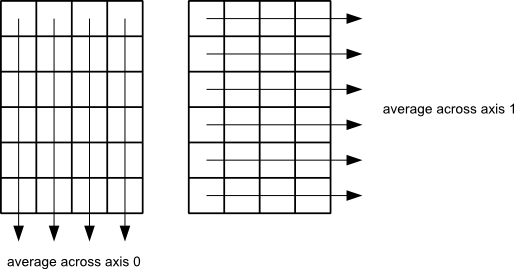
\includegraphics{novice/python/img/python-operations-across-axes.png}

To support this, most array methods allow us to specify the axis we want
to work on. If we ask for the average across axis 0, we get:

\begin{verbatim}
print data.mean(axis=0)
\end{verbatim}

\begin{verbatim}
[  0.           0.45         1.11666667   1.75         2.43333333   3.15
   3.8          3.88333333   5.23333333   5.51666667   5.95         5.9
   8.35         7.73333333   8.36666667   9.5          9.58333333
  10.63333333  11.56666667  12.35        13.25        11.96666667
  11.03333333  10.16666667  10.           8.66666667   9.15         7.25
   7.33333333   6.58333333   6.06666667   5.95         5.11666667   3.6
   3.3          3.56666667   2.48333333   1.5          1.13333333
   0.56666667]
\end{verbatim}

As a quick check, we can ask this array what its shape is:

\begin{verbatim}
print data.mean(axis=0).shape
\end{verbatim}

\begin{verbatim}
(40,)
\end{verbatim}

The expression \texttt{(40,)} tells us we have an N×1 vector, so this is
the average inflammation per day for all patients. If we average across
axis 1, we get:

\begin{verbatim}
print data.mean(axis=1)
\end{verbatim}

\begin{verbatim}
[ 5.45   5.425  6.1    5.9    5.55   6.225  5.975  6.65   6.625  6.525
  6.775  5.8    6.225  5.75   5.225  6.3    6.55   5.7    5.85   6.55
  5.775  5.825  6.175  6.1    5.8    6.425  6.05   6.025  6.175  6.55
  6.175  6.35   6.725  6.125  7.075  5.725  5.925  6.15   6.075  5.75
  5.975  5.725  6.3    5.9    6.75   5.925  7.225  6.15   5.95   6.275  5.7
  6.1    6.825  5.975  6.725  5.7    6.25   6.4    7.05   5.9  ]
\end{verbatim}

which is the average inflammation per patient across all days.

\begin{swcbox}{Slicing}
A subsection of an array is called a \gl{slice}{g:slice}. We can
take slices of character strings as well:

\begin{verbatim}
element = 'oxygen'
print 'first three characters:', element[0:3]
print 'last three characters:', element[3:6]
\end{verbatim}

\begin{verbatim}
first three characters: oxy
last three characters: gen
\end{verbatim}
\end{swcbox}

\begin{challenge}
  What is the value of \texttt{element{[}:4{]}}? What about
  \texttt{element{[}4:{]}}? Or \texttt{element{[}:{]}}?
\end{challenge}

\begin{challenge}
  What is \texttt{element{[}-1{]}}? What is \texttt{element{[}-2{]}}?
  Given those answers, explain what \texttt{element{[}1:-1{]}} does.
\end{challenge}

\begin{challenge}
  The expression \texttt{element{[}3:3{]}} produces an
  \gl{empty string}{g:empty-string}, i.e., a string that contains
  no characters. If \texttt{data} holds our array of patient data, what
  does \texttt{data{[}3:3, 4:4{]}} produce? What about
  \texttt{data{[}3:3, :{]}}?
\end{challenge}

\subsection{Plotting}

The mathematician Richard Hamming once said, ``The purpose of computing
is insight, not numbers,'' and the best way to develop insight is often
to visualize data. Visualization deserves an entire lecture (or course)
of its own, but we can explore a few features of Python's
\texttt{matplotlib} here. First, let's tell the IPython Notebook that we
want our plots displayed inline, rather than in a separate viewing
window:

\begin{verbatim}
%matplotlib inline
\end{verbatim}

The \texttt{\%} at the start of the line signals that this is a command
for the notebook, rather than a statement in Python. Next, we will
import the \texttt{pyplot} module from \texttt{matplotlib} and use two
of its functions to create and display a heat map of our data:

\begin{verbatim}
from matplotlib import pyplot
pyplot.imshow(data)
pyplot.show()
\end{verbatim}

\begin{verbatim}
\end{verbatim}

Blue regions in this heat map are low values, while red shows high
values. As we can see, inflammation rises and falls over a 40-day
period. Let's take a look at the average inflammation over time:

\begin{verbatim}
ave_inflammation = data.mean(axis=0)
pyplot.plot(ave_inflammation)
pyplot.show()
\end{verbatim}

\begin{verbatim}
\end{verbatim}

Here, we have put the average per day across all patients in the
variable \texttt{ave\_inflammation}, then asked \texttt{pyplot} to
create and display a line graph of those values. The result is roughly a
linear rise and fall, which is suspicious: based on other studies, we
expect a sharper rise and slower fall. Let's have a look at two other
statistics:

\begin{verbatim}
print 'maximum inflammation per day'
pyplot.plot(data.max(axis=0))
pyplot.show()

print 'minimum inflammation per day'
pyplot.plot(data.min(axis=0))
pyplot.show()
\end{verbatim}

\begin{verbatim}
maximum inflammation per day


minimum inflammation per day

\end{verbatim}

The maximum value rises and falls perfectly smoothly, while the minimum
seems to be a step function. Neither result seems particularly likely,
so either there's a mistake in our calculations or something is wrong
with our data.

\begin{challenge}
  Why do all of our plots stop just short of the upper end of our graph?
  Why are the vertical lines in our plot of the minimum inflammation per
  day not vertical?
\end{challenge}

\begin{challenge}
  Create a plot showing the standard deviation of the inflammation data
  for each day across all patients.
\end{challenge}

\subsection{Wrapping Up}

It's very common to create an \gl{alias}{g:alias-library} for a
library when importing it in order to reduce the amount of typing we
have to do. Here are our three plots side by side using aliases for
\texttt{numpy} and \texttt{pyplot}:

\begin{verbatim}
import numpy as np
from matplotlib import pyplot as plt

data = np.loadtxt(fname='inflammation-01.csv', delimiter=',')

plt.figure(figsize=(10.0, 3.0))

plt.subplot(1, 3, 1)
plt.ylabel('average')
plt.plot(data.mean(0))

plt.subplot(1, 3, 2)
plt.ylabel('max')
plt.plot(data.max(0))

plt.subplot(1, 3, 3)
plt.ylabel('min')
plt.plot(data.min(0))

plt.tight_layout()
plt.show()
\end{verbatim}

\begin{verbatim}
\end{verbatim}

The first two lines re-load our libraries as \texttt{np} and
\texttt{plt}, which are the aliases most Python programmers use. The
call to \texttt{loadtxt} reads our data, and the rest of the program
tells the plotting library how large we want the figure to be, that
we're creating three sub-plots, what to draw for each one, and that we
want a tight layout. (Perversely, if we leave out that call to
\texttt{plt.tight\_layout()}, the graphs will actually be squeezed
together more closely.)

\begin{challenge}
  Modify the program to display the three plots on top of one another
  instead of side by side.
\end{challenge}

\begin{keypoints}
\begin{swcitemize}
\item
  Import a library into a program using \texttt{import libraryname}.
\item
  Use the \texttt{numpy} library to work with arrays in Python.
\item
  Use \texttt{variable = value} to assign a value to a variable in order
  to record it in memory.
\item
  Variables are created on demand whenever a value is assigned to them.
\item
  Use \texttt{print something} to display the value of
  \texttt{something}.
\item
  The expression \texttt{array.shape} gives the shape of an array.
\item
  Use \texttt{array{[}x, y{]}} to select a single element from an array.
\item
  Array indices start at 0, not 1.
\item
  Use \texttt{low:high} to specify a slice that includes the indices
  from \texttt{low} to \texttt{high-1}.
\item
  All the indexing and slicing that works on arrays also works on
  strings.
\item
  Use \texttt{\# some kind of explanation} to add comments to programs.
\item
  Use \texttt{array.mean()}, \texttt{array.max()}, and
  \texttt{array.min()} to calculate simple statistics.
\item
  Use \texttt{array.mean(axis=0)} or \texttt{array.mean(axis=1)} to
  calculate statistics across the specified axis.
\item
  Use the \texttt{pyplot} library from \texttt{matplotlib} for creating
  simple visualizations.
\end{swcitemize}
\end{keypoints}

\mbox{}\paragraph{Next Steps}

Our work so far has convinced us that something's wrong with our first
data file. We would like to check the other 11 the same way, but typing
in the same commands repeatedly is tedious and error-prone. Since
computers don't get bored (that we know of), we should create a way to
do a complete analysis with a single command, and then figure out how to
repeat that step once for each file. These operations are the subjects
of the next two lessons.

\section{Creating Functions}

If we only had one data set to analyze, it would probably be faster to
load the file into a spreadsheet and use that to plot some simple
statistics. But we have twelve files to check, and may have more in
future. In this lesson, we'll learn how to write a function so that we
can repeat several operations with a single command.

\begin{objectives}
\begin{swcitemize}
\item
  Define a function that takes parameters.
\item
  Return a value from a function.
\item
  Test and debug a function.
\item
  Explain what a call stack is, and trace changes to the call stack as
  functions are called.
\item
  Set default values for function parameters.
\item
  Explain why we should divide programs into small, single-purpose
  functions.
\end{swcitemize}
\end{objectives}

\subsection{Defining a Function}

Let's start by defining a function \texttt{fahr\_to\_kelvin} that
converts temperatures from Fahrenheit to Kelvin:

\begin{verbatim}
def fahr_to_kelvin(temp):
    return ((temp - 32) * (5/9)) + 273.15
\end{verbatim}

The definition opens with the word \texttt{def}, which is followed by
the name of the function and a parenthesized list of parameter names.
The \gl{body}{g:function-body} of the function---the statements
that are executed when it runs---is indented below the definition line,
typically by four spaces.

When we call the function, the values we pass to it are assigned to
those variables so that we can use them inside the function. Inside the
function, we use a \gl{return statement}{g:return-statement} to
send a result back to whoever asked for it.

Let's try running our function. Calling our own function is no different
from calling any other function:

\begin{verbatim}
print 'freezing point of water:', fahr_to_kelvin(32)
print 'boiling point of water:', fahr_to_kelvin(212)
\end{verbatim}

\begin{verbatim}
freezing point of water: 273.15
boiling point of water: 273.15
\end{verbatim}

We've successfully called the function that we defined, and we have
access to the value that we returned. Unfortunately, the value returned
doesn't look right. What went wrong?

\subsection{Debugging a Function}

\emph{Debugging} is when we fix a piece of code that we know is working
incorrectly. In this case, we know that \texttt{fahr\_to\_kelvin} is
giving us the wrong answer, so let's find out why.

For big pieces of code, there are tools called \emph{debuggers} that aid
in this process.

We just have a short function, so we'll debug by choosing some parameter
value, breaking our function into small parts, and printing out the
value of each part.

\begin{verbatim}
# We'll use temp = 212, the boiling point of water, which was incorrect
print "212 - 32:", 212 - 32
\end{verbatim}

\begin{verbatim}
212 - 32: 180
\end{verbatim}

\begin{verbatim}
print "(212 - 32) * (5/9):", (212 - 32) * (5/9)
\end{verbatim}

\begin{verbatim}
(212 - 32) * (5/9): 0
\end{verbatim}

Aha! The problem comes when we multiply by \texttt{5/9}. This is because
\texttt{5/9} is actually 0.

\begin{verbatim}
5/9
\end{verbatim}

\begin{verbatim}
0
\end{verbatim}

Computers store numbers in one of two ways: as
\gl{integers}{g:integer} or as \gl{floating-point
numbers}{g:float} (or floats). The first are the numbers we usually count with;
the second have fractional parts. Addition, subtraction and
multiplication work on both as we'd expect, but division works
differently. If we divide one integer by another, we get the quotient
without the remainder:

\begin{verbatim}
print '10/3 is:', 10/3
\end{verbatim}

\begin{verbatim}
10/3 is: 3
\end{verbatim}

If either part of the division is a float, on the other hand, the
computer creates a floating-point answer:

\begin{verbatim}
print '10.0/3 is:', 10.0/3
\end{verbatim}

\begin{verbatim}
10.0/3 is: 3.33333333333
\end{verbatim}

The computer does this for historical reasons: integer operations were
much faster on early machines, and this behavior is actually useful in a
lot of situations. It's still confusing, though, so Python 3 produces a
floating-point answer when dividing integers if it needs to. We're still
using Python 2.7 in this class, though, so if we want \texttt{5/9} to
give us the right answer, we have to write it as \texttt{5.0/9},
\texttt{5/9.0}, or some other variation.

Let's fix our \texttt{fahr\_to\_kelvin} function with this new
knowledge.

\begin{verbatim}
def fahr_to_kelvin(temp):
    return ((temp - 32) * (5.0/9.0)) + 273.15

print 'freezing point of water:', fahr_to_kelvin(32)
print 'boiling point of water:', fahr_to_kelvin(212)
\end{verbatim}

\begin{verbatim}
freezing point of water: 273.15
boiling point of water: 373.15
\end{verbatim}

It works!

\subsection{Composing Functions}

Now that we've seen how to turn Fahrenheit into Kelvin, it's easy to
turn Kelvin into Celsius:

\begin{verbatim}
def kelvin_to_celsius(temp):
    return temp - 273.15

print 'absolute zero in Celsius:', kelvin_to_celsius(0.0)
\end{verbatim}

\begin{verbatim}
absolute zero in Celsius: -273.15
\end{verbatim}

What about converting Fahrenheit to Celsius? We could write out the
formula, but we don't need to. Instead, we can
\gl{compose}{g:function-composition} the two functions we have
already created:

\begin{verbatim}
def fahr_to_celsius(temp):
    temp_k = fahr_to_kelvin(temp)
    result = kelvin_to_celsius(temp_k)
    return result

print 'freezing point of water in Celsius:', fahr_to_celsius(32.0)
\end{verbatim}

\begin{verbatim}
freezing point of water in Celsius: 0.0
\end{verbatim}

This is our first taste of how larger programs are built: we define
basic operations, then combine them in ever-large chunks to get the
effect we want. Real-life functions will usually be larger than the ones
shown here---typically half a dozen to a few dozen lines---but they
shouldn't ever be much longer than that, or the next person who reads it
won't be able to understand what's going on.

\begin{challenge}
  ``Adding'' two strings produces their concatention: \texttt{'a' + 'b'}
  is \texttt{'ab'}. Write a function called \texttt{fence} that takes
  two parameters called \texttt{original} and \texttt{wrapper} and
  returns a new string that has the wrapper character at the beginning
  and end of the original:

\begin{verbatim}
print fence('name', '*')
*name*
\end{verbatim}
\end{challenge}

\begin{challenge}
  If the variable \texttt{s} refers to a string, then \texttt{s{[}0{]}}
  is the string's first character and \texttt{s{[}-1{]}} is its last.
  Write a function called \texttt{outer} that returns a string made up
  of just the first and last characters of its input:

\begin{verbatim}
print outer('helium')
hm
\end{verbatim}
\end{challenge}

\subsection{The Call Stack}

Let's take a closer look at what happens when we call
\texttt{fahr\_to\_celsius(32.0)}. To make things clearer, we'll start by
putting the initial value 32.0 in a variable and store the final result
in one as well:

\begin{verbatim}
original = 32.0
final = fahr_to_celsius(original)
\end{verbatim}

The diagram below shows what memory looks like after the first line has
been executed:

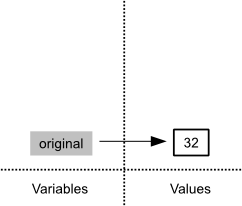
\includegraphics{novice/python/img/python-call-stack-01.png}

When we call \texttt{fahr\_to\_celsius}, Python \emph{doesn't} create
the variable \texttt{temp} right away. Instead, it creates something
called a \gl{stack frame}{g:stack-frame} to keep track of the
variables defined by \texttt{fahr\_to\_kelvin}. Initially, this stack
frame only holds the value of \texttt{temp}:

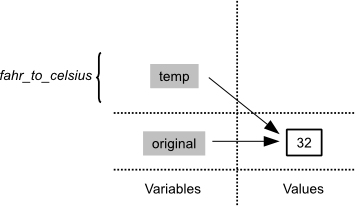
\includegraphics{novice/python/img/python-call-stack-02.png}

When we call \texttt{fahr\_to\_kelvin} inside
\texttt{fahr\_to\_celsius}, Python creates another stack frame to hold
\texttt{fahr\_to\_kelvin}'s variables:

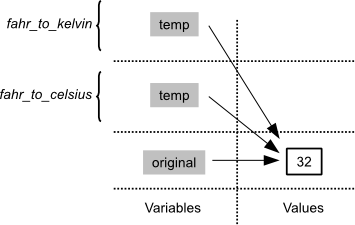
\includegraphics{novice/python/img/python-call-stack-03.png}

It does this because there are now two variables in play called
\texttt{temp}: the parameter to \texttt{fahr\_to\_celsius}, and the
parameter to \texttt{fahr\_to\_kelvin}. Having two variables with the
same name in the same part of the program would be ambiguous, so Python
(and every other modern programming language) creates a new stack frame
for each function call to keep that function's variables separate from
those defined by other functions.

When the call to \texttt{fahr\_to\_kelvin} returns a value, Python
throws away \texttt{fahr\_to\_kelvin}'s stack frame and creates a new
variable in the stack frame for \texttt{fahr\_to\_celsius} to hold the
temperature in Kelvin:

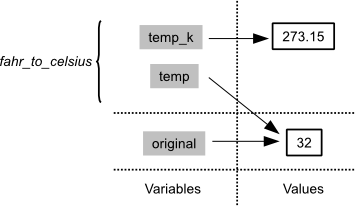
\includegraphics{novice/python/img/python-call-stack-04.png}

It then calls \texttt{kelvin\_to\_celsius}, which means it creates a
stack frame to hold that function's variables:

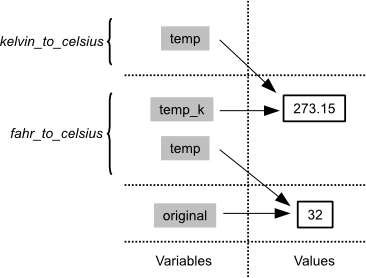
\includegraphics{novice/python/img/python-call-stack-05.png}

Once again, Python throws away that stack frame when
\texttt{kelvin\_to\_celsius} is done and creates the variable
\texttt{result} in the stack frame for \texttt{fahr\_to\_celsius}:

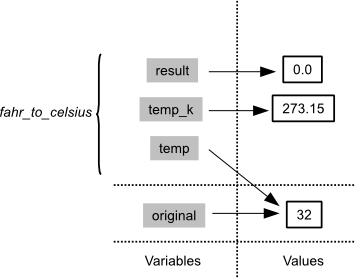
\includegraphics{novice/python/img/python-call-stack-06.png}

Finally, when \texttt{fahr\_to\_celsius} is done, Python throws away
\emph{its} stack frame and puts its result in a new variable called
\texttt{final} that lives in the stack frame we started with:

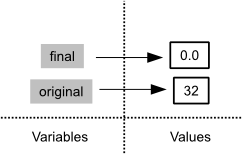
\includegraphics{novice/python/img/python-call-stack-07.png}

This final stack frame is always there; it holds the variables we
defined outside the functions in our code. What it \emph{doesn't} hold
is the variables that were in the various stack frames. If we try to get
the value of \texttt{temp} after our functions have finished running,
Python tells us that there's no such thing:

\begin{verbatim}
print 'final value of temp after all function calls:', temp
\end{verbatim}

\begin{verbatim}
---------------------------------------------------------------------------
NameError                                 Traceback (most recent call last)
<ipython-input-12-ffd9b4dbd5f1> in <module>()
----> 1 print 'final value of temp after all function calls:', temp

NameError: name 'temp' is not definedfinal value of temp after all function calls:
\end{verbatim}

Why go to all this trouble? Well, here's a function called \texttt{span}
that calculates the difference between the mininum and maximum values in
an array:

\begin{verbatim}
import numpy

def span(a):
    diff = a.max() - a.min()
    return diff

data = numpy.loadtxt(fname='inflammation-01.csv', delimiter=',')
print 'span of data', span(data)
\end{verbatim}

\begin{verbatim}
 span of data 20.0
\end{verbatim}

Notice that \texttt{span} assigns a value to a variable called
\texttt{diff}. We might very well use a variable with the same name to
hold data:

\begin{verbatim}
diff = numpy.loadtxt(fname='inflammation-01.csv', delimiter=',')
print 'span of data:', span(diff)
\end{verbatim}

\begin{verbatim}
span of data: 20.0
\end{verbatim}

We don't expect \texttt{diff} to have the value 20.0 after this function
call, so the name \texttt{diff} cannot refer to the same thing inside
\texttt{span} as it does in the main body of our program. And yes, we
could probably choose a different name than \texttt{diff} in our main
program in this case, but we don't want to have to read every line of
NumPy to see what variable names its functions use before calling any of
those functions, just in case they change the values of our variables.

The big idea here is \gl{encapsulation}{g:encapsulation}, and it's
the key to writing correct, comprehensible programs. A function's job is
to turn several operations into one so that we can think about a single
function call instead of a dozen or a hundred statements each time we
want to do something. That only works if functions don't interfere with
each other; if they do, we have to pay attention to the details once
again, which quickly overloads our short-term memory.

\begin{challenge}
  We previously wrote functions called \texttt{fence} and
  \texttt{outer}. Draw a diagram showing how the call stack changes when
  we run the following:
\begin{verbatim}
print outer(fence('carbon', `+'))
\end{verbatim}
\end{challenge}

\subsection{Testing and Documenting}

Once we start putting things in functions so that we can re-use them, we
need to start testing that those functions are working correctly. To see
how to do this, let's write a function to center a dataset around a
particular value:

\begin{verbatim}
def center(data, desired):
    return (data - data.mean()) + desired
\end{verbatim}

We could test this on our actual data, but since we don't know what the
values ought to be, it will be hard to tell if the result was correct.
Instead, let's use NumPy to create a matrix of 0's and then center that
around 3:

\begin{verbatim}
z = numpy.zeros((2,2))
print center(z, 3)
\end{verbatim}

\begin{verbatim}
[[ 3.  3.]
 [ 3.  3.]]
\end{verbatim}

That looks right, so let's try \texttt{center} on our real data:

\begin{verbatim}
data = numpy.loadtxt(fname='inflammation-01.csv', delimiter=',')
print center(data, 0)
\end{verbatim}

\begin{verbatim}
[[-6.14875 -6.14875 -5.14875 ..., -3.14875 -6.14875 -6.14875]
 [-6.14875 -5.14875 -4.14875 ..., -5.14875 -6.14875 -5.14875]
 [-6.14875 -5.14875 -5.14875 ..., -4.14875 -5.14875 -5.14875]
 ...,
 [-6.14875 -5.14875 -5.14875 ..., -5.14875 -5.14875 -5.14875]
 [-6.14875 -6.14875 -6.14875 ..., -6.14875 -4.14875 -6.14875]
 [-6.14875 -6.14875 -5.14875 ..., -5.14875 -5.14875 -6.14875]]
\end{verbatim}

It's hard to tell from the default output whether the result is correct,
but there are a few simple tests that will reassure us:

\begin{verbatim}
print 'original min, mean, and max are:', data.min(), data.mean(), data.max()
centered = center(data, 0)
print 'min, mean, and and max of centered data are:', centered.min(), centered.mean(), centered.max()
\end{verbatim}

\begin{verbatim}
original min, mean, and max are: 0.0 6.14875 20.0
min, mean, and and max of centered data are: -6.14875 -3.49054118942e-15 13.85125
\end{verbatim}

That seems almost right: the original mean was about 6.1, so the lower
bound from zero is how about -6.1. The mean of the centered data isn't
quite zero---we'll explore why not in the challenges---but it's pretty
close. We can even go further and check that the standard deviation
hasn't changed:

\begin{verbatim}
print 'std dev before and after:', data.std(), centered.std()
\end{verbatim}

\begin{verbatim}
std dev before and after: 4.61383319712 4.61383319712
\end{verbatim}

Those values look the same, but we probably wouldn't notice if they were
different in the sixth decimal place. Let's do this instead:

\begin{verbatim}
print 'difference in standard deviations before and after:', data.std() - centered.std()
\end{verbatim}

\begin{verbatim}
difference in standard deviations before and after: -3.5527136788e-15
\end{verbatim}

Again, the difference is very small. It's still possible that our
function is wrong, but it seems unlikely enough that we should probably
get back to doing our analysis. We have one more task first, though: we
should write some \gl{documentation}{g:documentation} for our
function to remind ourselves later what it's for and how to use it.

The usual way to put documentation in software is to add
\gl{comments}{g:comment} like this:

\begin{verbatim}
# center(data, desired): return a new array containing the original data centered around the desired value.
def center(data, desired):
    return (data - data.mean()) + desired
\end{verbatim}

There's a better way, though. If the first thing in a function is a
string that isn't assigned to a variable, that string is attached to the
function as its documentation:

\begin{verbatim}
def center(data, desired):
    '''Return a new array containing the original data centered around the desired value.'''
    return (data - data.mean()) + desired
\end{verbatim}

This is better because we can now ask Python's built-in help system to
show us the documentation for the function:

\begin{verbatim}
help(center)
\end{verbatim}

\begin{verbatim}
Help on function center in module __main__:

center(data, desired)
    Return a new array containing the original data centered around the desired value.
\end{verbatim}

A string like this is called a \gl{docstring}{g:docstring}. We
don't need to use triple quotes when we write one, but if we do, we can
break the string across multiple lines:

\begin{verbatim}
def center(data, desired):
    '''Return a new array containing the original data centered around the desired value.
    Example: center([1, 2, 3], 0) => [-1, 0, 1]'''
    return (data - data.mean()) + desired

help(center)
\end{verbatim}

\begin{verbatim}
Help on function center in module __main__:

center(data, desired)
    Return a new array containing the original data centered around the desired value.
    Example: center([1, 2, 3], 0) => [-1, 0, 1]
\end{verbatim}

\begin{challenge}
  Write a function called \texttt{analyze} that takes a filename as a
  parameter and displays the three graphs produced in the
  \urlfoot{01-numpy.ipynb}{previous lesson}, i.e.,
  \texttt{analyze('inflammation-01.csv')} should produce the graphs
  already shown, while \texttt{analyze('inflammation-02.csv')} should
  produce corresponding graphs for the second data set. Be sure to give
  your function a docstring.
\end{challenge}

\begin{challenge}
  Write a function \texttt{rescale} that takes an array as input and
  returns a corresponding array of values scaled to lie in the range 0.0
  to 1.0. (If \textbackslash{}(L\textbackslash{}) and
  \textbackslash{}(H\textbackslash{}) are the lowest and highest values
  in the original array, then the replacement for a value
  \textbackslash{}(v\textbackslash{}) should be \textbackslash{}((v-L) /
  (H-L)\textbackslash{}).) Be sure to give the function a docstring.
\end{challenge}

\begin{challenge}
  Run the commands \texttt{help(numpy.arange)} and
  \texttt{help(numpy.linspace)} to see how to use these functions to
  generate regularly-spaced values, then use those values to test your
  \texttt{rescale} function.
\end{challenge}

\subsection{Defining Defaults}

We have passed parameters to functions in two ways: directly, as in
\texttt{span(data)}, and by name, as in
\texttt{numpy.loadtxt(fname='something.csv', delimiter=',')}. In fact,
we can pass the filename to \texttt{loadtxt} without the
\texttt{fname=}:

\begin{verbatim}
numpy.loadtxt('inflammation-01.csv', delimiter=',')
\end{verbatim}

\begin{verbatim}
array([[ 0.,  0.,  1., ...,  3.,  0.,  0.],
       [ 0.,  1.,  2., ...,  1.,  0.,  1.],
       [ 0.,  1.,  1., ...,  2.,  1.,  1.],
       ...,
       [ 0.,  1.,  1., ...,  1.,  1.,  1.],
       [ 0.,  0.,  0., ...,  0.,  2.,  0.],
       [ 0.,  0.,  1., ...,  1.,  1.,  0.]])
\end{verbatim}

but we still need to say \texttt{delimiter=}:

\begin{verbatim}
numpy.loadtxt('inflammation-01.csv', ',')
\end{verbatim}

\begin{verbatim}
---------------------------------------------------------------------------
TypeError                                 Traceback (most recent call last)
<ipython-input-26-e3bc6cf4fd6a> in <module>()
----> 1 numpy.loadtxt('inflammation-01.csv', ',')

/Users/gwilson/anaconda/lib/python2.7/site-packages/numpy/lib/npyio.pyc in loadtxt(fname, dtype, comments, delimiter, converters, skiprows, usecols, unpack, ndmin)
    775     try:
    776         # Make sure we're dealing with a proper dtype
--> 777         dtype = np.dtype(dtype)
    778         defconv = _getconv(dtype)
    779

TypeError: data type "," not understood
\end{verbatim}

To understand what's going on, and make our own functions easier to use,
let's re-define our \texttt{center} function like this:

\begin{verbatim}
def center(data, desired=0.0):
    '''Return a new array containing the original data centered around the desired value (0 by default).
    Example: center([1, 2, 3], 0) => [-1, 0, 1]'''
    return (data - data.mean()) + desired
\end{verbatim}

The key change is that the second parameter is now written
\texttt{desired=0.0} instead of just \texttt{desired}. If we call the
function with two arguments, it works as it did before:

\begin{verbatim}
test_data = numpy.zeros((2, 2))
print center(test_data, 3)
\end{verbatim}

\begin{verbatim}
[[ 3.  3.]
 [ 3.  3.]]
\end{verbatim}

But we can also now call it with just one parameter, in which case
\texttt{desired} is automatically assigned the
\gl{default value}{g:default-parameter-value} of 0.0:

\begin{verbatim}
more_data = 5 + numpy.zeros((2, 2))
print 'data before centering:', more_data
print 'centered data:', center(more_data)
\end{verbatim}

\begin{verbatim}
data before centering: [[ 5.  5.]
 [ 5.  5.]]
centered data: [[ 0.  0.]
 [ 0.  0.]]
\end{verbatim}

This is handy: if we usually want a function to work one way, but
occasionally need it to do something else, we can allow people to pass a
parameter when they need to but provide a default to make the normal
case easier. The example below shows how Python matches values to
parameters:

\begin{verbatim}
def display(a=1, b=2, c=3):
    print 'a:', a, 'b:', b, 'c:', c

print 'no parameters:'
display()
print 'one parameter:'
display(55)
print 'two parameters:'
display(55, 66)
\end{verbatim}

\begin{verbatim}
no parameters:
a: 1 b: 2 c: 3
one parameter:
a: 55 b: 2 c: 3
two parameters:
a: 55 b: 66 c: 3
\end{verbatim}

As this example shows, parameters are matched up from left to right, and
any that haven't been given a value explicitly get their default value.
We can override this behavior by naming the value as we pass it in:

\begin{verbatim}
print 'only setting the value of c'
display(c=77)
\end{verbatim}

\begin{verbatim}
only setting the value of c
a: 1 b: 2 c: 77
\end{verbatim}

With that in hand, let's look at the help for \texttt{numpy.loadtxt}:

\begin{verbatim}
help(numpy.loadtxt)
\end{verbatim}

\begin{verbatim}
Help on function loadtxt in module numpy.lib.npyio:

loadtxt(fname, dtype=<type 'float'>, comments='#', delimiter=None, converters=None, skiprows=0, usecols=None, unpack=False, ndmin=0)
    Load data from a text file.

    Each row in the text file must have the same number of values.

    Parameters
    ----------
    fname : file or str
        File, filename, or generator to read.  If the filename extension is
        ``.gz`` or ``.bz2``, the file is first decompressed. Note that
        generators should return byte strings for Python 3k.
    dtype : data-type, optional
        Data-type of the resulting array; default: float.  If this is a
        record data-type, the resulting array will be 1-dimensional, and
        each row will be interpreted as an element of the array.  In this
        case, the number of columns used must match the number of fields in
        the data-type.
    comments : str, optional
        The character used to indicate the start of a comment;
        default: '#'.
    delimiter : str, optional
        The string used to separate values.  By default, this is any
        whitespace.
    converters : dict, optional
        A dictionary mapping column number to a function that will convert
        that column to a float.  E.g., if column 0 is a date string:
        ``converters = {0: datestr2num}``.  Converters can also be used to
        provide a default value for missing data (but see also `genfromtxt`):
        ``converters = {3: lambda s: float(s.strip() or 0)}``.  Default: None.
    skiprows : int, optional
        Skip the first `skiprows` lines; default: 0.
    usecols : sequence, optional
        Which columns to read, with 0 being the first.  For example,
        ``usecols = (1,4,5)`` will extract the 2nd, 5th and 6th columns.
        The default, None, results in all columns being read.
    unpack : bool, optional
        If True, the returned array is transposed, so that arguments may be
        unpacked using ``x, y, z = loadtxt(...)``.  When used with a record
        data-type, arrays are returned for each field.  Default is False.
    ndmin : int, optional
        The returned array will have at least `ndmin` dimensions.
        Otherwise mono-dimensional axes will be squeezed.
        Legal values: 0 (default), 1 or 2.
        .. versionadded:: 1.6.0

    Returns
    -------
    out : ndarray
        Data read from the text file.

    See Also
    --------
    load, fromstring, fromregex
    genfromtxt : Load data with missing values handled as specified.
    scipy.io.loadmat : reads MATLAB data files

    Notes
    -----
    This function aims to be a fast reader for simply formatted files.  The
    `genfromtxt` function provides more sophisticated handling of, e.g.,
    lines with missing values.

    Examples
    --------
    >>> from StringIO import StringIO   # StringIO behaves like a file object
    >>> c = StringIO("0 1\n2 3")
    >>> np.loadtxt(c)
    array([[ 0.,  1.],
           [ 2.,  3.]])

    >>> d = StringIO("M 21 72\nF 35 58")
    >>> np.loadtxt(d, dtype={'names': ('gender', 'age', 'weight'),
    ...                      'formats': ('S1', 'i4', 'f4')})
    array([('M', 21, 72.0), ('F', 35, 58.0)],
          dtype=[('gender', '|S1'), ('age', '<i4'), ('weight', '<f4')])

    >>> c = StringIO("1,0,2\n3,0,4")
    >>> x, y = np.loadtxt(c, delimiter=',', usecols=(0, 2), unpack=True)
    >>> x
    array([ 1.,  3.])
    >>> y
    array([ 2.,  4.])
\end{verbatim}

There's a lot of information here, but the most important part is the
first couple of lines:

\begin{verbatim}
loadtxt(fname, dtype=<type 'float'>, comments='#', delimiter=None, converters=None, skiprows=0, usecols=None,
        unpack=False, ndmin=0)
\end{verbatim}

This tells us that \texttt{loadtxt} has one parameter called
\texttt{fname} that doesn't have a default value, and eight others that
do. If we call the function like this:

\begin{verbatim}
numpy.loadtxt('inflammation-01.csv', ',')
\end{verbatim}

then the filename is assigned to \texttt{fname} (which is what we want),
but the delimiter string \texttt{','} is assigned to \texttt{dtype}
rather than \texttt{delimiter}, because \texttt{dtype} is the second
parameter in the list. That's why we don't have to provide
\texttt{fname=} for the filename, but \emph{do} have to provide
\texttt{delimiter=} for the second parameter.

\begin{challenge}
  Rewrite the \texttt{center} function so that it scales data to lie
  between 0.0 and 1.0 by default, but will allow the caller to specify
  lower and upper bounds if they want. Compare your implementation to
  your neighbor's: do the two functions always behave the same way?
\end{challenge}

\begin{keypoints}
\begin{swcitemize}
\item
  Define a function using \texttt{def name(...params...)}.
\item
  The body of a function must be indented.
\item
  Call a function using \texttt{name(...values...)}.
\item
  Numbers are stored as integers or floating-point numbers.
\item
  Integer division produces the whole part of the answer (not the
  fractional part).
\item
  Each time a function is called, a new stack frame is created on the
  \gl{call stack}{g:call-stack} to hold its parameters and local
  variables.
\item
  Python looks for variables in the current stack frame before looking
  for them at the top level.
\item
  Use \texttt{help(thing)} to view help for something.
\item
  Put docstrings in functions to provide help for that function.
\item
  Specify default values for parameters when defining a function using
  \texttt{name=value} in the parameter list.
\item
  Parameters can be passed by matching based on name, by position, or by
  omitting them (in which case the default value is used).
\end{swcitemize}
\end{keypoints}

\mbox{}\paragraph{Next Steps}

We now have a function called \texttt{analyze} to visualize a single
data set. We could use it to explore all 12 of our current data sets
like this:

\begin{verbatim}
analyze('inflammation-01.csv')
analyze('inflammation-02.csv')
...
analyze('inflammation-12.csv')
\end{verbatim}

but the chances of us typing all 12 filenames correctly aren't great,
and we'll be even worse off if we get another hundred files. What we
need is a way to tell Python to do something once for each file, and
that will be the subject of the next lesson.

\section{Analyzing Multiple Data Sets}

We have created a function called \texttt{analyze} that creates graphs
of the minimum, average, and maximum daily inflammation rates for a
single data set:

\begin{verbatim}
%matplotlib inline

import numpy as np
from matplotlib import pyplot as plt

def analyze(filename):
    data = np.loadtxt(fname=filename, delimiter=',')

    plt.figure(figsize=(10.0, 3.0))

    plt.subplot(1, 3, 1)
    plt.ylabel('average')
    plt.plot(data.mean(0))

    plt.subplot(1, 3, 2)
    plt.ylabel('max')
    plt.plot(data.max(0))

    plt.subplot(1, 3, 3)
    plt.ylabel('min')
    plt.plot(data.min(0))

    plt.tight_layout()
    plt.show()

analyze('inflammation-01.csv')
\end{verbatim}

\begin{verbatim}
\end{verbatim}

We can use it to analyze other data sets one by one:

\begin{verbatim}
analyze('inflammation-02.csv')
\end{verbatim}

\begin{verbatim}
\end{verbatim}

but we have a dozen data sets right now and more on the way. We want to
create plots for all our data sets with a single statement. To do that,
we'll have to teach the computer how to repeat things.

\begin{objectives}
\begin{swcitemize}
\item
  Explain what a for loop does.
\item
  Correctly write for loops to repeat simple calculations.
\item
  Trace changes to a loop variable as the loop runs.
\item
  Trace changes to other variables as they are updated by a for loop.
\item
  Explain what a list is.
\item
  Create and index lists of simple values.
\item
  Use a library function to get a list of filenames that match a simple
  wildcard pattern.
\item
  Use a for loop to process multiple files.
\end{swcitemize}
\end{objectives}

\subsection{For Loops}

Suppose we want to print each character in the word ``lead'' on a line
of its own. One way is to use four \texttt{print} statements:

\begin{verbatim}
def print_characters(element):
    print element[0]
    print element[1]
    print element[2]
    print element[3]

print_characters('lead')
\end{verbatim}

\begin{verbatim}
l
e
a
d
\end{verbatim}

but that's a bad approach for two reasons:

\begin{swcenumerate}
\item
  It doesn't scale: if we want to print the characters in a string
  that's hundreds of letters long, we'd be better off just typing them
  in.
\item
  It's fragile: if we give it a longer string, it only prints part of
  the data, and if we give it a shorter one, it produces an error
  because we're asking for characters that don't exist.
\end{swcenumerate}

\begin{verbatim}
print_characters('tin')
\end{verbatim}

\begin{verbatim}
---------------------------------------------------------------------------
IndexError                                Traceback (most recent call last)
<ipython-input-13-5bc7311e0bf3> in <module>()
----> 1 print_characters('tin')

<ipython-input-12-11460561ea56> in print_characters(element)
      3     print element[1]
      4     print element[2]
----> 5     print element[3]
      6
      7 print_characters('lead')

IndexError: string index out of ranget
i
n
\end{verbatim}

Here's a better approach:

\begin{verbatim}
def print_characters(element):
    for char in element:
        print char

print_characters('lead')
\end{verbatim}

This is shorter---certainly shorter than something that prints every
character in a hundred-letter string---and more robust as well:

\begin{verbatim}
print_characters('oxygen')
\end{verbatim}

The improved version of \texttt{print\_characters} uses a
\gl{for loop}{g:for-loop} to repeat an operation---in this case,
printing---once for each thing in a collection. The general form of a
loop is:

\begin{verbatim}
for variable in collection:
    do things with variable
\end{verbatim}

We can call the \gl{loop variable}{g:loop-variable} anything we
like, but there must be a colon at the end of the line starting the
loop, and we must indent the body of the loop.

Here's another loop that repeatedly updates a variable:

\begin{verbatim}
length = 0
for vowel in 'aeiou':
    length = length + 1
print 'There are', length, 'vowels'
\end{verbatim}

It's worth tracing the execution of this little program step by step.
Since there are five characters in \texttt{'aeiou'}, the statement on
line 3 will be executed five times. The first time around,
\texttt{length} is zero (the value assigned to it on line 1) and
\texttt{vowel} is \texttt{'a'}. The statement adds 1 to the old value of
\texttt{length}, producing 1, and updates \texttt{length} to refer to
that new value. The next time around, \texttt{vowel} is \texttt{'e'} and
\texttt{length} is 1, so \texttt{length} is updated to be 2. After three
more updates, \texttt{length} is 5; since there is nothing left in
\texttt{'aeiou'} for Python to process, the loop finishes and the
\texttt{print} statement on line 4 tells us our final answer.

Note that a loop variable is just a variable that's being used to record
progress in a loop. It still exists after the loop is over, and we can
re-use variables previously defined as loop variables as well:

\begin{verbatim}
letter = 'z'
for letter in 'abc':
    print letter
print 'after the loop, letter is', letter
\end{verbatim}

Note also that finding the length of a string is such a common operation
that Python actually has a built-in function to do it called
\texttt{len}:

\begin{verbatim}
print len('aeiou')
\end{verbatim}

\texttt{len} is much faster than any function we could write ourselves,
and much easier to read than a two-line loop; it will also give us the
length of many other things that we haven't met yet, so we should always
use it when we can.

\begin{challenge}
  Python has a built-in function called \texttt{range} that creates a
  list of numbers: \texttt{range(3)} produces \texttt{{[}0, 1, 2{]}},
  \texttt{range(2, 5)} produces \texttt{{[}2, 3, 4{]}}, and
  \texttt{range(2, 10, 3)} produces \texttt{{[}2, 5, 8{]}}. Using
  \texttt{range}, write a function that prints the
  \textbackslash{}(N\textbackslash{}) natural numbers:
\begin{verbatim}
print_N(3)
1 2 3
\end{verbatim}
\end{challenge}

\begin{challenge}
  Exponentiation is built into Python:
\begin{verbatim}
print 2**4
16
\end{verbatim}
  It also has a function called
  \texttt{pow} that calculates the same value. Write a function called
  \texttt{expo} that uses a loop to calculate the same result.
\end{challenge}

\begin{challenge}
  Python's strings have methods, just like NumPy's arrays. One of these
  is called \texttt{reverse}:
\begin{verbatim}
  print `Newton'.reverse()
notweN
\end{verbatim}
  Write a function called \texttt{rev} that does the same thing:
\begin{verbatim}
print rev('Newton')
notweN
\end{verbatim}
  As always, be sure to include a
  docstring.
\end{challenge}

\subsection{Lists}

Just as a \texttt{for} loop is a way to do operations many times, a list
is a way to store many values. Unlike NumPy arrays, there are built into
the language. We create a list by putting values inside square brackets:

\begin{verbatim}
odds = [1, 3, 5, 7]
print 'odds are:', odds
\end{verbatim}

We select individual elements from lists by indexing them:

\begin{verbatim}
print 'first and last:', odds[0], odds[-1]
\end{verbatim}

and if we loop over a list, the loop variable is assigned elements one
at a time:

\begin{verbatim}
for number in odds:
    print number
\end{verbatim}

There is one important difference between lists and strings: we can
change the values in a list, but we cannot change the characters in a
string. For example:

\begin{verbatim}
names = ['Newton', 'Darwing', 'Turing'] # typo in Darwin's name
print 'names is originally:', names
names[1] = 'Darwin' # correct the name
print 'final value of names:', names
\end{verbatim}

works, but:

\begin{verbatim}
name = 'Bell'
name[0] = 'b'
\end{verbatim}

does not.

\begin{swcbox}{Ch-Ch-Ch-Changes}

Data that can be changed is called \gl{mutable}{g:mutable}, while
data that cannot be is called \gl{immutable}{g:immutable}. Like
strings, numbers are immutable: there's no way to make the number 0 have
the value 1 or vice versa (at least, not in Python---there actually
\emph{are} languages that will let people do this, with predictably
confusing results). Lists and arrays, on the other hand, are mutable:
both can be modified after they have been created.

Programs that modify data in place can be harder to understand than ones
that don't because readers may have to mentally sum up many lines of
code in order to figure out what the value of something actually is. On
the other hand, programs that modify data in place instead of creating
copies that are almost identical to the original every time they want to
make a small change are much more efficient.

\end{swcbox}

There are many ways to change the contents of in lists besides assigning
to elements:

\begin{verbatim}
odds.append(11)
print 'odds after adding a value:', odds
\end{verbatim}

\begin{verbatim}
del odds[0]
print 'odds after removing the first element:', odds
\end{verbatim}

\begin{verbatim}
odds.reverse()
print 'odds after reversing:', odds
\end{verbatim}

\begin{challenge}
  Write a function called \texttt{total} that calculates the sum of the
  values in a list. (Python has a built-in function called \texttt{sum}
  that does this for you. Please don't use it for this exercise.)
\end{challenge}

\subsection{Processing Multiple Files}

We now have almost everything we need to process all our data files. The
only thing that's missing is a library with a rather unpleasant name:

\begin{verbatim}
import glob
\end{verbatim}

The \texttt{glob} library contains a single function, also called
\texttt{glob}, that finds files whose names match a pattern. We provide
those patterns as strings: the character \texttt{*} matches zero or more
characters, while \texttt{?} matches any one character. We can use this
to get the names of all the IPython Notebooks we have created so far:

\begin{verbatim}
print glob.glob('*.ipynb')
\end{verbatim}

\begin{verbatim}
['01-numpy.ipynb', '02-func.ipynb', '03-loop.ipynb', '04-cond.ipynb', '05-defensive.ipynb', '06-cmdline.ipynb', 'spatial-intro.ipynb']
\end{verbatim}

or to get the names of all our CSV data files:

\begin{verbatim}
print glob.glob('*.csv')
\end{verbatim}

\begin{verbatim}
['inflammation-01.csv', 'inflammation-02.csv', 'inflammation-03.csv', 'inflammation-04.csv', 'inflammation-05.csv', 'inflammation-06.csv', 'inflammation-07.csv', 'inflammation-08.csv', 'inflammation-09.csv', 'inflammation-10.csv', 'inflammation-11.csv', 'inflammation-12.csv', 'small-01.csv', 'small-02.csv', 'small-03.csv', 'swc_bc_coords.csv']
\end{verbatim}

As these examples show, \texttt{glob.glob}'s result is a list of
strings, which means we can loop over it to do something with each
filename in turn. In our case, the ``something'' we want is our
\texttt{analyze} function. Let's test it by analyzing the first three
files in the list:

\begin{verbatim}
filenames = glob.glob('*.csv')
filenames = filenames[0:3]
for f in filenames:
    print f
    analyze(f)
\end{verbatim}

\begin{verbatim}
inflammation-01.csv


inflammation-02.csv


inflammation-03.csv

\end{verbatim}

Sure enough, the maxima of these data sets show exactly the same ramp as
the first, and their minima show the same staircase structure.

\begin{challenge}
  Write a function called \texttt{analyze\_all} that takes a filename
  pattern as its sole argument and runs \texttt{analyze} for each file
  whose name matches the pattern.
\end{challenge}

\begin{keypoints}
\begin{swcitemize}
\item
  Use \texttt{for variable in collection} to process the elements of a
  collection one at a time.
\item
  The body of a for loop must be indented.
\item
  Use \texttt{len(thing)} to determine the length of something that
  contains other values.
\item
  \texttt{{[}value1, value2, value3, ...{]}} creates a list.
\item
  Lists are indexed and sliced in the same way as strings and arrays.
\item
  Lists are mutable (i.e., their values can be changed in place).
\item
  Strings are immutable (i.e., the characters in them cannot be
  changed).
\item
  Use \texttt{glob.glob(pattern)} to create a list of files whose names
  match a pattern.
\item
  Use \texttt{*} in a pattern to match zero or more characters, and
  \texttt{?} to match any single character.
\end{swcitemize}
\end{keypoints}

\mbox{}\paragraph{Next Steps}

We have now solved our original problem: we can analyze any number of
data files with a single command. More importantly, we have met two of
the most important ideas in programming:

\begin{swcenumerate}
\item
  Use functions to make code easier to re-use and easier to understand.
\item
  Use lists and arrays to store related values, and loops to repeat
  operations on them.
\end{swcenumerate}

We have one more big idea to introduce, and then we will be able to go
back and create a heat map like the one we initially used to display our
first data set.

\section{Making Choices}

Our previous lessons have shown us how to manipulate data, define our
own functions, and repeat things. However, the programs we have written
so far always do the same things, regardless of what data they're given.
We want programs to make choices based on the values they are
manipulating. To help us see what decisions they're making, we'll start
by looking at how computers manipulate images.

\begin{objectives}
\begin{swcitemize}
\item
  Create a simple ``image'' made out of colored blocks.
\item
  Explain how the RGB model represents colors.
\item
  Explain the similarities and differences between tuples and lists.
\item
  Write conditional statements including \texttt{if}, \texttt{elif}, and
  \texttt{else} branches.
\item
  Correctly evaluate expressions containing \texttt{and} and
  \texttt{or}.
\item
  Correctly write and interpret code containing nested loops and
  conditionals.
\item
  Explain the advantages of putting frequently-modified code in a
  function.
\end{swcitemize}
\end{objectives}

\subsection{Image Grids}

Let's start by creating some simple heat maps of our own using a library
called \texttt{ipythonblocks}. The first step is to create our own
``image'':

\begin{verbatim}
from ipythonblocks import ImageGrid
\end{verbatim}

Unlike the \texttt{import} statements we have seen earlier, this one
doesn't load the entire \texttt{ipythonblocks} library. Instead, it just
loads \texttt{ImageGrid} from that library, since that's the only thing
we need (for now).

Once we have \texttt{ImageGrid} loaded, we can use it to create a very
simple grid of colored cells:

\begin{verbatim}
grid = ImageGrid(5, 3)
grid.show()
\end{verbatim}

\begin{verbatim}
table.blockgrid {border: none;} .blockgrid tr {border: none;} .blockgrid td {padding: 0px;} #blocks84e827e4-60f2-4e82-b41a-c95955a972aa td {border: 1px solid white;}
\end{verbatim}

Just like a NumPy array, an \texttt{ImageGrid} has some properties that
hold information about it:

\begin{verbatim}
print 'grid width:', grid.width
print 'grid height:', grid.height
print 'grid lines on:', grid.lines_on
\end{verbatim}

\begin{verbatim}
grid width: 5
grid height: 3
grid lines on: True
\end{verbatim}

The obvious thing to do with a grid like this is color in its cells, but
in order to do that, we need to know how computers represent color. The
most common schemes are \gl{RGB}{g:rgb}, which is short for ``red,
green, blue''. RGB is an \gl{additive
color model}{g:additive-color-model}: every shade is some combination of red, green, and blue
intensities. We can think of these three values as being the axes in a
cube:

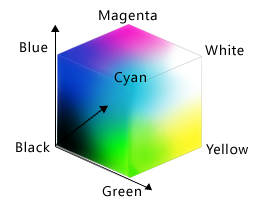
\includegraphics{novice/python/img/color-cube.png}

An RGB color is an example of a multi-part value: like a Cartesian
coordinate, it is one thing with several parts. We can represent such a
value in Python using a \gl{tuple}{g:tuple}, which we write using
parentheses instead of the square brackets used for a list:

\begin{verbatim}
position = (12.3, 45.6)
print 'position is:', position
color = (10, 20, 30)
print 'color is:', color
\end{verbatim}

\begin{verbatim}
position is: (12.3, 45.6)
color is: (10, 20, 30)
\end{verbatim}

We can select elements from tuples using indexing, just as we do with
lists and arrays:

\begin{verbatim}
print 'first element of color is:', color[0]
\end{verbatim}

\begin{verbatim}
first element of color is: 10
\end{verbatim}

Unlike lists and arrays, though, tuples cannot be changed after they are
created---in technical terms, they are
\gl{immutable}{g:immutable}:

\begin{verbatim}
color[0] = 40
print 'first element of color after change:', color[0]
\end{verbatim}

\begin{verbatim}
---------------------------------------------------------------------------
TypeError                                 Traceback (most recent call last)
<ipython-input-11-9c3dd30a4e52> in <module>()
----> 1 color[0] = 40
      2 print 'first element of color after change:', color[0]

TypeError: 'tuple' object does not support item assignment
\end{verbatim}

If a tuple represents an RGB color, its red, green, and blue components
can take on values between 0 and 255. The upper bound may seem odd, but
it's the largest number that can be represented in an 8-bit byte (i.e.,
2\textsuperscript{8}-1). This makes it easy for computers to manipulate
colors, while providing fine enough gradations to fool most human eyes,
most of the time.

Let's see what a few RGB colors actually look like:

\begin{verbatim}
row = ImageGrid(8, 1)
row[0, 0] = (0, 0, 0)   # no color => black
row[1, 0] = (255, 255, 255) # all colors => white
row[2, 0] = (255, 0, 0) # all red
row[3, 0] = (0, 255, 0) # all green
row[4, 0] = (0, 0, 255) # all blue
row[5, 0] = (255, 255, 0) # red and green
row[6, 0] = (255, 0, 255) # red and blue
row[7, 0] = (0, 255, 255) # green and blue
row.show()
\end{verbatim}

\begin{verbatim}
table.blockgrid {border: none;} .blockgrid tr {border: none;} .blockgrid td {padding: 0px;} #blocks9d1f4bb1-553c-4074-aec0-dc48fde66e06 td {border: 1px solid white;}
\end{verbatim}

Simple color values like \texttt{(0,255,0)} are easy enough to decipher
with a bit of practice, but what color is \texttt{(214,90,127)}? To help
us, \texttt{ipythonblocks} provides a function called
\texttt{show\_color}:

\begin{verbatim}
from ipythonblocks import show_color
show_color(214, 90, 127)
\end{verbatim}

\begin{verbatim}
\end{verbatim}

It also provides a table of standard colors:

\begin{verbatim}
from ipythonblocks import colors
c = ImageGrid(3, 2)
c[0, 0] = colors['Fuchsia']
c[0, 1] = colors['Salmon']
c[1, 0] = colors['Orchid']
c[1, 1] = colors['Lavender']
c[2, 0] = colors['LimeGreen']
c[2, 1] = colors['HotPink']
c.show()
\end{verbatim}

\begin{verbatim}
table.blockgrid {border: none;} .blockgrid tr {border: none;} .blockgrid td {padding: 0px;} #blocksb8c954b3-f908-4ab1-8013-65bf49ec1b2f td {border: 1px solid white;}
\end{verbatim}

\begin{challenge}
  Fill in the \texttt{\_\_\_\_} in the code below to create a bar that
  changes color from dark blue to black.

\begin{verbatim}
bar = ImageGrid(10, 1)
for x in range(10):
    bar[x, 0] = (0, 0, ____)
bar.show()
\end{verbatim}
\end{challenge}

\begin{challenge}
  Why do computers use red, green, and blue as their primary colors?
\end{challenge}

\subsection{Conditionals}

The other thing we need in order to create a heat map of our own is a
way to pick a color based on a data value. The tool Python gives us for
doing this is called a \gl{conditional
statement}{g:conditional-statement}, and looks like this:

\begin{verbatim}
num = 37
if num > 100:
    print 'greater'
else:
    print 'not greater'
print 'done'
\end{verbatim}

\begin{verbatim}
not greater
done
\end{verbatim}

The second line of this code uses the keyword \texttt{if} to tell Python
that we want to make a choice. If the test that follows it is true, the
body of the \texttt{if} (i.e., the lines indented underneath it) are
executed. If the test is false, the body of the \texttt{else} is
executed instead. Only one or the other is ever executed:

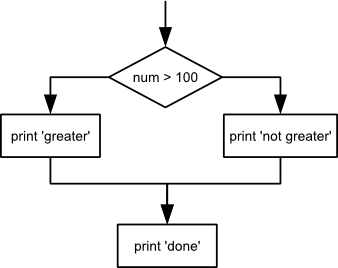
\includegraphics{novice/python/img/python-flowchart-conditional.png}

Conditional statements don't have to include an \texttt{else}. If there
isn't one, Python simply does nothing if the test is false:

\begin{verbatim}
num = 53
print 'before conditional...'
if num > 100:
    print '53 is greater than 100'
print '...after conditional'
\end{verbatim}

\begin{verbatim}
before conditional...
...after conditional
\end{verbatim}

We can also chain several tests together using \texttt{elif}, which is
short for ``else if''. This makes it simple to write a function that
returns the sign of a number:

\begin{verbatim}
def sign(num):
    if num > 0:
        return 1
    elif num == 0:
        return 0
    else:
        return -1

print 'sign of -3:', sign(-3)
\end{verbatim}

\begin{verbatim}
sign of -3: -1
\end{verbatim}

One important thing to notice the code above is that we use a double
equals sign \texttt{==} to test for equality rather than a single equals
sign because the latter is used to mean assignment. This convention was
inherited from C, and while many other programming languages work the
same way, it does take a bit of getting used to\ldots{}

We can also combine tests using \texttt{and} and \texttt{or}.
\texttt{and} is only true if both parts are true:

\begin{verbatim}
if (1 > 0) and (-1 > 0):
    print 'both parts are true'
else:
    print 'one part is not true'
\end{verbatim}

\begin{verbatim}
one part is not true
\end{verbatim}

while \texttt{or} is true if either part is true:

\begin{verbatim}
if (1 < 0) or ('left' < 'right'):
    print 'at least one test is true'
\end{verbatim}

\begin{verbatim}
at least one test is true
\end{verbatim}

In this case, ``either'' means ``either or both'', not ``either one or
the other but not both''.

\begin{challenge}
  \texttt{True} and \texttt{False} aren't the only values in Python that
  are true and false. In fact, \emph{any} value can be used in an
  \texttt{if} or \texttt{elif}. After reading and running the code
  below, explain what the rule is for which values are considered true
  and which are considered false. (Note that if the body of a
  conditional is a single statement, we can write it on the same line as
  the \texttt{if}.)

\begin{verbatim}
if '': print 'empty string is true'
if 'word': print 'word is true'
if []: print 'empty list is true'
if [1, 2, 3]: print 'non-empty list is true'
if 0: print 'zero is true'
if 1: print 'one is true'
\end{verbatim}
\end{challenge}

\begin{challenge}
  Write a function called \texttt{near} that returns \texttt{True} if
  its first parameter is within 10\% of its second and \texttt{False}
  otherwise. Compare your implementation with your partner's: do you
  return the same answer for all possible pairs of numbers?
\end{challenge}

\subsection{Nesting}

Another thing to realize is that \texttt{if} statements can be combined
with loops just as easily as they can be combined with functions. For
example, if we want to sum the positive numbers in a list, we can write
this:

\begin{verbatim}
numbers = [-5, 3, 2, -1, 9, 6]
total = 0
for n in numbers:
    if n >= 0:
        total = total + n
print 'sum of positive values:', total
\end{verbatim}

\begin{verbatim}
sum of positive values: 20
\end{verbatim}

We could equally well calculate the positive and negative sums in a
single loop:

\begin{verbatim}
pos_total = 0
neg_total = 0
for n in numbers:
    if n >= 0:
        pos_total = pos_total + n
    else:
        neg_total = neg_total + n
print 'negative and positive sums are:', neg_total, pos_total
\end{verbatim}

\begin{verbatim}
negative and positive sums are: -6 20
\end{verbatim}

We can even put one loop inside another:

\begin{verbatim}
for consonant in 'bcd':
    for vowel in 'ae':
        print consonant + vowel
\end{verbatim}

\begin{verbatim}
ba
be
ca
ce
da
de
\end{verbatim}

As the diagram below shows, the \gl{inner loop}{g:inner-loop} runs
from start to finish each time the \gl{outer loop}{g:outer-loop}
runs once:

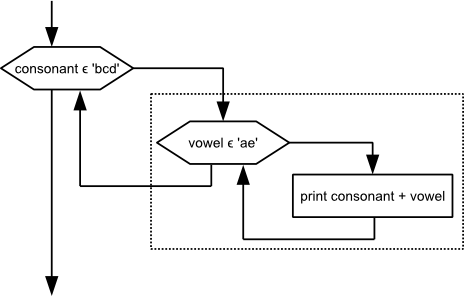
\includegraphics{novice/python/img/python-flowchart-nested-loops.png}

We can combine nesting and conditionals to create patterns in an image:

\begin{verbatim}
square = ImageGrid(5, 5)
for x in range(square.width):
    for y in range(square.height):
        if x < y:
            square[x, y] = colors['Fuchsia']
        elif x == y:
            square[x, y] = colors['Olive']
        else:
            square[x, y] = colors['SlateGray']
square.show()
\end{verbatim}

\begin{verbatim}
table.blockgrid {border: none;} .blockgrid tr {border: none;} .blockgrid td {padding: 0px;} #blocksa391625e-64d4-47e1-a54a-2953c1aea09c td {border: 1px solid white;}
\end{verbatim}

This is our first hand-made data visualization: the colors show where
\texttt{x} is less than, equal to, or greater than \texttt{y}.

\begin{challenge}
  Will changing the nesting of the loops in the code above---i.e.,
  wrapping the Y-axis loop around the X-axis loop---change the final
  image? Why or why not?
\end{challenge}

\begin{challenge}
  Python (and most other languages in the C family) provides
  \gl{in-place operators}{g:in-place-operator} that work like
  this:

\begin{verbatim}
x = 1  # original value
x += 1 # add one to x, assigning result back to x
x *= 3 # multiply x by 3
print x
6
\end{verbatim}

  Rewrite the code that sums the positive and negative numbers in a list
  using in-place operators. Do you think the result is more or less
  readable than the original?
\end{challenge}

\subsection{Creating a Heat Map}

The last step is to turn our data into something we can see. As in
previous lessons, the first step is to get the data into memory:

\begin{verbatim}
import numpy as np
data = np.loadtxt(fname='inflammation-01.csv', delimiter=',')
print 'data shape:', data.shape
\end{verbatim}

\begin{verbatim}
data shape: (60, 40)
\end{verbatim}

The second is to create an image grid that is the same size as the data:

\begin{verbatim}
width, height = data.shape
heatmap = ImageGrid(width, height)
\end{verbatim}

(The first line of the code above takes advantage of a neat trick: we
can unpack the values in a tuple by assigning it to as many variables as
it has entries.)

The third step is to decide \emph{how} we are going to color the cells
in the heat map. To keep things simple, we will use red, green, and blue
as our colors, and compare data values to the data set's mean. Here's
the code:

\begin{verbatim}
for x in range(width):
    for y in range(height):
        if data[x, y] < data.mean():
            heatmap[x, y] = colors['Red']
        elif data[x, y] == data.mean():
            heatmap[x, y] = colors['Green']
        else:
            heatmap[x, y] = colors['Blue']
heatmap.show()
\end{verbatim}

\begin{verbatim}
table.blockgrid {border: none;} .blockgrid tr {border: none;} .blockgrid td {padding: 0px;} #blocks1cdd8344-bb95-4b16-bc13-b4fb6f13235a td {border: 1px solid white;}
\end{verbatim}

This may be what we asked for, but both the image and the code are
hideous:

\begin{swcenumerate}
\item
  It's too large for us to view the whole thing at once on a small
  laptop screen.
\item
  Our first heatmap had time along the X axis; this seems to have time
  along the Y axis.
\item
  Red against blue is pretty hard on the eyes.
\item
  The heatmap only shows two colors because none of the (integer)
  measurements has exactly the same value as the (fractional) mean.
\item
  We are calculating the mean of \texttt{data} either once or twice each
  time we go through the loop. That means that on a 40×60 data set, we
  are performing the same calculation 2400 times.
\end{swcenumerate}

Here's how we can improve it:

\begin{swcenumerate}
\item
  We can give \texttt{ImageGrid} an optional parameter
  \texttt{block\_size} to set the size of each block.
\item
  We can transpose our data before creating the grid.
\item
  We can pick better colors (I'm personally fond of orchid, fuchsia, and
  hot pink).
\item
  Instead of checking if values are exactly equal to the mean, we can
  see if they are close to it.
\item
  We can calculate the mean once, before we start our loops, and use
  that value over and over.
\end{swcenumerate}

Our modified code looks like this:

\begin{verbatim}
flipped = data.transpose()
width, height = flipped.shape
heatmap = ImageGrid(width, height, block_size=5)
center = flipped.mean()
for x in range(width):
    for y in range(height):
        if flipped[x, y] < (0.8 * center):
            heatmap[x, y] = colors['Orchid']
        elif flipped[x, y] > (1.2 * center):
            heatmap[x, y] = colors['HotPink']
        else:
            heatmap[x, y] = colors['Fuchsia']
heatmap.show()
\end{verbatim}

\begin{verbatim}
table.blockgrid {border: none;} .blockgrid tr {border: none;} .blockgrid td {padding: 0px;} #blocksa46f17da-750a-4616-8173-7dfb16227fb8 td {border: 1px solid white;}
\end{verbatim}

That's a bit better---but now the contrast between the colors isn't
great enough. And there still aren't very many fuchsia cells: we may
want to widen the band around the mean that gets that color.

We could rewrite our loop a third time, but the right thing to do is to
put our code in a function so that we can experiment with bands and
colors more easily.

\begin{verbatim}
def make_heatmap(values, low_color, mid_color, high_color, low_band, high_band, block_size):
    '''Make a 3-colored heatmap from a 2D array of data.'''
    width, height = values.shape
    result = ImageGrid(width, height, block_size=block_size)
    center = values.mean()
    for x in range(width):
        for y in range(height):
            if values[x, y] < low_band * center:
                result[x, y] = low_color
            elif values[x, y] > high_band * center:
                result[x, y] = high_color
            else:
                result[x, y] = mid_color
    return result
\end{verbatim}

To test this function, we'll run it with the settings we just used:

\begin{verbatim}
h = make_heatmap(flipped, colors['Orchid'], colors['Fuchsia'], colors['HotPink'], 0.8, 1.2, 5)
h.show()
\end{verbatim}

\begin{verbatim}
table.blockgrid {border: none;} .blockgrid tr {border: none;} .blockgrid td {padding: 0px;} #blocks01f46f8f-ce3d-4e60-810e-14913fdd0249 td {border: 1px solid white;}
\end{verbatim}

That seems right, so let's widen the band and use more dramatic colors:

\begin{verbatim}
h = make_heatmap(flipped, colors['Gray'], colors['YellowGreen'], colors['SpringGreen'], 0.5, 1.5, 5)
h.show()
\end{verbatim}

\begin{verbatim}
table.blockgrid {border: none;} .blockgrid tr {border: none;} .blockgrid td {padding: 0px;} #blocks934bdfbe-fa39-46bc-951f-e504b83c5ed2 td {border: 1px solid white;}
\end{verbatim}

We'll probably want to experiment a bit more before publishing, but
writing a function has made experimenting easy. We can make it even
easier by re-defining our function one more time to give the parameters
default values. While we're at it, let's put the low and high bands at
the front, since they're more likely to change than our color choices:

\begin{verbatim}
def make_heatmap(values,
                 low_band=0.5, high_band=1.5,
                 low_color=colors['Gray'], mid_color=colors['YellowGreen'], high_color=colors['SpringGreen'],
                 block_size=5):
    '''Make a 3-colored heatmap from a 2D array of data.
    Default color scheme is gray to green.'''
    width, height = values.shape
    result = ImageGrid(width, height, block_size=block_size)
    center = values.mean()
    for x in range(width):
        for y in range(height):
            if values[x, y] < low_band * center:
                result[x, y] = low_color
            elif values[x, y] > high_band * center:
                result[x, y] = high_color
            else:
                result[x, y] = mid_color
    return result
\end{verbatim}

Once default values are added, the function's first line is too long to
fit comfortably on our screen. Rather than breaking it wherever it hits
the right edge of the screen, we have divided the parameters into
logical groups to make it more readable.

Again, our first test is to re-run it with the same values as before
(which we give it in a different order, since we've changed the order of
parameters):

\begin{verbatim}
h = make_heatmap(flipped, 0.5, 1.5, colors['Gray'], colors['YellowGreen'], colors['SpringGreen'], 5)
h.show()
\end{verbatim}

\begin{verbatim}
table.blockgrid {border: none;} .blockgrid tr {border: none;} .blockgrid td {padding: 0px;} #blocks68bc8298-2807-40bb-8077-cb6a6c133f91 td {border: 1px solid white;}
\end{verbatim}

We can now leave out everything except the data being visualized, or
provide the data and the bands and re-use the default colors and block
size:

\begin{verbatim}
h = make_heatmap(flipped, 0.4, 1.6)
h.show()
\end{verbatim}

\begin{verbatim}
table.blockgrid {border: none;} .blockgrid tr {border: none;} .blockgrid td {padding: 0px;} #blocks3a6cb5f4-cba3-448a-b130-320fed0e64e4 td {border: 1px solid white;}
\end{verbatim}

We can now explore our data with just a few keystrokes, which means we
can concentrate on our science and not on our programming.

\begin{challenge}
  Why did we transpose our data outside our heat map function? Why not
  have the function perform the transpose?
\end{challenge}

\begin{challenge}
  Why does the heat map function return the grid rather than displaying
  it immediately? Do you think this is a good or bad design choice?
\end{challenge}

\begin{challenge}
  Explain what the overall effect of this code is:
\begin{verbatim}
temp = left
left = right
right = temp
\end{verbatim}
Compare it to:
\begin{verbatim}
left, right = right, left
\end{verbatim}
  Do they always do the same thing?
  Which do you find easier to read?
\end{challenge}

\begin{keypoints}
\begin{swcitemize}
\item
  Use the \texttt{ImageGrid} class from the \texttt{ipythonblocks}
  library to create simple ``images'' made of colored blocks.
\item
  Specify colors use (red, green, blue) triples, each component of which
  is an integer in the range 0..255.
\item
  Use \texttt{if condition} to start a conditional statement,
  \texttt{elif condition} to provide additional tests, and \texttt{else}
  to provide a default.
\item
  The bodies of the branches of conditional statements must be indented.
\item
  Use \texttt{==} to test for equality.
\item
  \texttt{X and Y} is only true if both X and Y are true.
\item
  \texttt{X or Y} is true if either X or Y, or both, are true.
\item
  Zero, the empty string, and the empty list are considered false; all
  other numbers, strings, and lists are considered true.
\item
  Nest loops to operate on multi-dimensional data.
\item
  Put code whose parameters change frequently in a function, then call
  it with different parameter values to customize its behavior.
\end{swcitemize}
\end{keypoints}

\mbox{}\paragraph{Next Steps}

Our final heatmap function is 17 lines long, which means that if there's
a 95\% chance of each line being correct, the odds of the whole function
being right are only 41\%. Before we go any further, we need to learn
how to test whether our code is doing what we want it to do, and that
will be the subject of the next lesson.

\section{Defensive Programming}

Our previous lessons have introduced the basic tools of programming:
variables and lists, file I/O, loops, conditionals, and functions. What
they \emph{haven't} done is show us how to tell whether a program is
getting the right answer, and how to tell if it's \emph{still} getting
the right answer as we make changes to it.

To achieve that, we need to:

\begin{swcitemize}
\item
  write programs that check their own operation,
\item
  write and run tests for widely-used functions, and
\item
  make sure we know what ``correct'' actually means.
\end{swcitemize}

The good news is, doing these things will speed up our programming, not
slow it down. As in real carpentry---the kind done with lumber---the
time saved by measuring carefully before cutting a piece of wood is much
greater than the time that measuring takes.

\begin{objectives}
\begin{swcitemize}
\item
  Explain what an assertion is.
\item
  Add assertions to programs that correctly check the program's state.
\item
  Correctly add precondition and postcondition assertions to functions.
\item
  Explain what test-driven development is, and use it when creating new
  functions.
\item
  Explain why variables should be initialized using actual data values
  rather than arbitrary constants.
\item
  Debug code containing an error systematically.
\end{swcitemize}
\end{objectives}

\subsection{Assertions}

The first step toward getting the right answers from our programs is to
assume that mistakes \emph{will} happen and to guard against them. This
is called \gl{defensive programming}{g:defensive-programming}, and
the most common way to do it is to add
\gl{assertions}{g:assertion} to our code so that it checks itself
as it runs. An assertion is simply a statement that something must be
true at a certain point in a program. When Python sees one, it checks
that the assertion's condition. If it's true, Python does nothing, but
if it's false, Python halts the program immediately and prints the error
message provided. For example, this piece of code halts as soon as the
loop encounters a value that isn't positive:

\begin{verbatim}
numbers = [1.5, 2.3, 0.7, -0.001, 4.4]
total = 0.0
for n in numbers:
    assert n >= 0.0, 'Data should only contain positive values'
    total += n
print 'total is:', total
\end{verbatim}

\begin{verbatim}
---------------------------------------------------------------------------
AssertionError                            Traceback (most recent call last)
<ipython-input-3-33d87ea29ae4> in <module>()
      2 total = 0.0
      3 for n in numbers:
----> 4     assert n >= 0.0, 'Data should only contain positive values'
      5     total += n
      6 print 'total is:', total

AssertionError: Data should only contain positive values
\end{verbatim}

Programs like the Firefox browser are full of assertions: 10-20\% of the
code they contain are there to check that the other 80-90\% are working
correctly. Broadly speaking, assertions fall into three categories:

\begin{swcitemize}
\item
  A \gl{precondition}{g:precondition} is something that must be
  true at the start of a function in order for it to work correctly.
\item
  A \gl{postcondition}{g:postcondition} is something that the
  function guarantees is true when it finishes.
\item
  An \gl{invariant}{g:invariant} is something that is always true
  at a particular point inside a piece of code.
\end{swcitemize}

For example, suppose we are representing rectangles using a tuple of
four coordinates \texttt{(x0, y0, x1, y1)}. In order to do some
calculations, we need to normalize the rectangle so that it is at the
origin and 1.0 units long on its longest axis. This function does that,
but checks that its input is correctly formatted and that its result
makes sense:

\begin{verbatim}
def normalize_rectangle(rect):
    '''Normalizes a rectangle so that it is at the origin and 1.0 units long on its longest axis.'''
    assert len(rect) == 4, 'Rectangles must contain 4 coordinates'
    x0, y0, x1, y1 = rect
    assert x0 < x1, 'Invalid X coordinates'
    assert y0 < y1, 'Invalid Y coordinates'

    dx = x1 - x0
    dy = y1 - y0
    if dx > dy:
        scaled = float(dx) / dy
        upper_x, upper_y = 1.0, scaled
    else:
        scaled = float(dx) / dy
        upper_x, upper_y = scaled, 1.0

    assert 0 < upper_x <= 1.0, 'Calculated upper X coordinate invalid'
    assert 0 < upper_y <= 1.0, 'Calculated upper Y coordinate invalid'

    return (0, 0, upper_x, upper_y)
\end{verbatim}

The preconditions on lines 2, 4, and 5 catch invalid inputs:

\begin{verbatim}
print normalize_rectangle( (0.0, 1.0, 2.0) ) # missing the fourth coordinate
\end{verbatim}

\begin{verbatim}
---------------------------------------------------------------------------
AssertionError                            Traceback (most recent call last)
<ipython-input-5-3a97b1dcab70> in <module>()
----> 1 print normalize_rectangle( (0.0, 1.0, 2.0) ) # missing the fourth coordinate

<ipython-input-4-9f8adbfdcfc9> in normalize_rectangle(rect)
      1 def normalize_rectangle(rect):
      2     '''Normalizes a rectangle so that it is at the origin and 1.0 units long on its longest axis.'''
----> 3     assert len(rect) == 4, 'Rectangles must contain 4 coordinates'
      4     x0, y0, x1, y1 = rect
      5     assert x0 < x1, 'Invalid X coordinates'

AssertionError: Rectangles must contain 4 coordinates
\end{verbatim}

\begin{verbatim}
print normalize_rectangle( (4.0, 2.0, 1.0, 5.0) ) # X axis inverted
\end{verbatim}

\begin{verbatim}
---------------------------------------------------------------------------
AssertionError                            Traceback (most recent call last)
<ipython-input-6-f05ae7878a45> in <module>()
----> 1 print normalize_rectangle( (4.0, 2.0, 1.0, 5.0) ) # X axis inverted

<ipython-input-4-9f8adbfdcfc9> in normalize_rectangle(rect)
      3     assert len(rect) == 4, 'Rectangles must contain 4 coordinates'
      4     x0, y0, x1, y1 = rect
----> 5     assert x0 < x1, 'Invalid X coordinates'
      6     assert y0 < y1, 'Invalid Y coordinates'
      7

AssertionError: Invalid X coordinates
\end{verbatim}

The post-conditions help us catch bugs by telling us when our
calculations cannot have been correct. For example, if we normalize a
rectangle that is taller than it is wide everything seems OK:

\begin{verbatim}
print normalize_rectangle( (0.0, 0.0, 1.0, 5.0) )
\end{verbatim}

\begin{verbatim}
(0, 0, 0.2, 1.0)
\end{verbatim}

but if we normalize one that's wider than it is tall, the assertion is
triggered:

\begin{verbatim}
print normalize_rectangle( (0.0, 0.0, 5.0, 1.0) )
\end{verbatim}

\begin{verbatim}
---------------------------------------------------------------------------
AssertionError                            Traceback (most recent call last)
<ipython-input-8-5f0ef7954aeb> in <module>()
----> 1 print normalize_rectangle( (0.0, 0.0, 5.0, 1.0) )

<ipython-input-4-9f8adbfdcfc9> in normalize_rectangle(rect)
     16
     17     assert 0 < upper_x <= 1.0, 'Calculated upper X coordinate invalid'
---> 18     assert 0 < upper_y <= 1.0, 'Calculated upper Y coordinate invalid'
     19
     20     return (0, 0, upper_x, upper_y)

AssertionError: Calculated upper Y coordinate invalid
\end{verbatim}

Re-reading our function, we realize that line 10 should divide
\texttt{dy} by \texttt{dx} rather than \texttt{dx} by \texttt{dy}. (You
can display line numbers by typing Ctrl-M, then L.) If we had left out
the assertion at the end of the function, we would have created and
returned something that had the right shape as a valid answer, but
wasn't. Detecting and debugging that would almost certainly have taken
more time in the long run than writing the assertion.

But assertions aren't just about catching errors: they also help people
understand programs. Each assertion gives the person reading the program
a chance to check (consciously or otherwise) that their understanding
matches what the code is doing.

Most good programmers follow two rules when adding assertions to their
code. The first is, ``\urlfoot{../../rules.html\#fail-early-fail-often}{fail
early, fail often}''. The greater the distance between when and where an
error occurs and when it's noticed, the harder the error will be to
debug, so good code catches mistakes as early as possible.

The second rule is,
``\urlfoot{../../rules.html\#turn-bugs-into-assertions-or-tests}{turn bugs
into assertions or tests}''. If you made a mistake in a piece of code,
the odds are good that you have made other mistakes nearby, or will make
the same mistake (or a related one) the next time you change it. Writing
assertions to check that you haven't \gl{regressed}{g:regression}
(i.e., haven't re-introduced an old problem) can save a lot of time in
the long run, and helps to warn people who are reading the code
(including your future self) that this bit is tricky.

\begin{challenge}
  Suppose you are writing a function called \texttt{average} that
  calculates the average of the numbers in a list. What pre-conditions
  and post-conditions would you write for it? Compare your answer to
  your neighbor's: can you think of a function that will past your tests
  but not hers or vice versa?
\end{challenge}

\begin{challenge}
  Explain in words what the assertions in this code check, and for each
  one, give an example of input that will make that assertion fail.

\begin{verbatim}
def running(values):
    assert len(values) > 0
    result = [values[0]]
    for v in values[1:]:
        assert result[-1] >= 0
        result.append(result[-1] + v)
    assert result[-1] >= result[0]
    return result
\end{verbatim}
\end{challenge}

\subsection{Test-Driven Development}

An assertion checks that something is true at a particular point in the
program. The next step is to check the overall behavior of a piece of
code, i.e., to make sure that it produces the right output when it's
given a particular input. For example, suppose we need to find where two
or more time series overlap. The range of each time series is
represented as a pair of numbers, which are the time the interval
started and ended. The output is the largest range that they all
include:

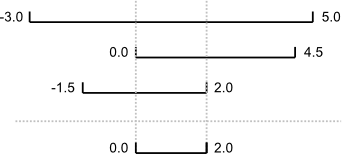
\includegraphics{novice/python/img/python-overlapping-ranges.png}

Most novice programmers would solve this problem like this:

\begin{swcenumerate}
\item
  Write a function \texttt{range\_overlap}.
\item
  Call it interactively on two or three different inputs.
\item
  If it produces the wrong answer, fix the function and re-run that
  test.
\end{swcenumerate}

This clearly works---after all, thousands of scientists are doing it
right now---but there's a better way:

\begin{swcenumerate}
\item
  Write a short function for each test.
\item
  Write a \texttt{range\_overlap} function that should pass those tests.
\item
  If \texttt{range\_overlap} produces any wrong answers, fix it and
  re-run the test functions.
\end{swcenumerate}

Writing the tests \emph{before} writing the function they exercise is
called \gl{test-driven development}{g:test-driven-development}
(TDD). Its advocates believe it produces better code faster because:

\begin{swcenumerate}
\item
  If people write tests after writing the thing to be tested, they are
  subject to confirmation bias, i.e., they subconsciously write tests to
  show that their code is correct, rather than to find errors.
\item
  Writing tests helps programmers figure out what the function is
  actually supposed to do.
\end{swcenumerate}

Here are three test functions for \texttt{range\_overlap}:

\begin{verbatim}
assert range_overlap([ (0.0, 1.0) ]) == (0.0, 1.0)
assert range_overlap([ (0.0, 1.0), (0.0, 2.0) ]) == (0.0, 1.0)
assert range_overlap([ (0.0, 1.0), (0.0, 2.0), (-1.0, 1.0) ]) == (0.0, 1.0)
\end{verbatim}

The error is actually reassuring: we haven't written
\texttt{range\_overlap} yet, so if the tests passed, it would be a sign
that someone else had and that we were accidentally using their
function.

And as a bonus of writing these tests, we've implicitly defined what our
input and output look like: we expect a list of pairs as input, and
produce a single pair as output.

Something important is missing, though. We don't have any tests for the
case where the ranges don't overlap at all:

\begin{verbatim}
assert range_overlap([ (0.0, 1.0), (5.0, 6.0) ]) == ???
\end{verbatim}

What should \texttt{range\_overlap} do in this case: fail with an error
message, produce a special value like \texttt{(0.0, 0.0)} to signal that
there's no overlap, or something else? Any actual implementation of the
function will do one of these things; writing the tests first helps us
figure out which is best \emph{before} we're emotionally invested in
whatever we happened to write before we realized there was an issue.

And what about this case?

\begin{verbatim}
assert range_overlap([ (0.0, 1.0), (1.0, 2.0) ]) == ???
\end{verbatim}

Do two segments that touch at their endpoints overlap or not?
Mathematicians usually say ``yes'', but engineers usually say ``no''.
The best answer is ``whatever is most useful in the rest of our
program'', but again, any actual implementation of
\texttt{range\_overlap} is going to do \emph{something}, and whatever it
is ought to be consistent with what it does when there's no overlap at
all.

Since we're planning to use the range this function returns as the X
axis in a time series chart, we decide that:

\begin{swcenumerate}
\item
  every overlap has to have non-zero width, and
\item
  we will return the special value \texttt{None} when there's no
  overlap.
\end{swcenumerate}

\texttt{None} is built into Python, and means ``nothing here''. (Other
languages often call the equivalent value \texttt{null} or
\texttt{nil}). With that decision made, we can finish writing our last
two tests:

\begin{verbatim}
assert range_overlap([ (0.0, 1.0), (5.0, 6.0) ]) == None
assert range_overlap([ (0.0, 1.0), (1.0, 2.0) ]) == None
\end{verbatim}

\begin{verbatim}
---------------------------------------------------------------------------
AssertionError                            Traceback (most recent call last)
<ipython-input-10-d877ef460ba2> in <module>()
----> 1 assert range_overlap([ (0.0, 1.0), (5.0, 6.0) ]) == None
      2 assert range_overlap([ (0.0, 1.0), (1.0, 2.0) ]) == None

AssertionError: 
\end{verbatim}

Again, we get an error because we haven't written our function, but
we're now ready to do so:

\begin{verbatim}
def range_overlap(ranges):
    '''Return common overlap among a set of [low, high] ranges.'''
    lowest = 0.0
    highest = 1.0
    for (low, high) in ranges:
        lowest = max(lowest, low)
        highest = min(highest, high)
    return (lowest, highest)
\end{verbatim}

(Take a moment to think about why we use \texttt{max} to raise
\texttt{lowest} and \texttt{min} to lower \texttt{highest}.) We'd now
like to re-run our tests, but they're scattered across three different
cells. To make running them easier, let's put them all in a function:

\begin{verbatim}
def test_range_overlap():
    assert range_overlap([ (0.0, 1.0) ]) == (0.0, 1.0)
    assert range_overlap([ (0.0, 1.0), (0.0, 2.0) ]) == (0.0, 1.0)
    assert range_overlap([ (0.0, 1.0), (0.0, 2.0), (-1.0, 1.0) ]) == (0.0, 1.0)
    assert range_overlap([ (0.0, 1.0), (5.0, 6.0) ]) == None
    assert range_overlap([ (0.0, 1.0), (1.0, 2.0) ]) == None
\end{verbatim}

We can now test \texttt{range\_overlap} with a single function call:

\begin{verbatim}
test_range_overlap()
\end{verbatim}

\begin{verbatim}
---------------------------------------------------------------------------
AssertionError                            Traceback (most recent call last)
<ipython-input-13-cf9215c96457> in <module>()
----> 1 test_range_overlap()

<ipython-input-12-34c3659163fc> in test_range_overlap()
      3     assert range_overlap([ (0.0, 1.0), (0.0, 2.0) ]) == (0.0, 1.0)
      4     assert range_overlap([ (0.0, 1.0), (0.0, 2.0), (-1.0, 1.0) ]) == (0.0, 1.0)
----> 5     assert range_overlap([ (0.0, 1.0), (5.0, 6.0) ]) == None
      6     assert range_overlap([ (0.0, 1.0), (1.0, 2.0) ]) == None

AssertionError: 
\end{verbatim}

The first of the tests that was supposed to produce \texttt{None} fails,
so we know there's something wrong with our function. What we
\emph{don't} know, though, is whether the last of our five tests passed
or failed, because Python halted the program as soon as it spotted the
first error. Still, some information is better than none, and if we
trace the behavior of the function with that input, we realize that
we're initializing \texttt{lowest} and \texttt{highest} to 0.0 and 1.0
respectively, regardless of the input values. This violates another
important rule of programming:
``\urlfoot{../../rules.html\#always-initialize-from-data}{always initialize
from data}''. We'll leave it as an exercise to fix
\texttt{range\_overlap}.

\begin{challenge}
  Fix \texttt{range\_overlap}. Re-run \texttt{test\_range\_overlap}
  after each change you make.
\end{challenge}

\subsection{Debugging}

Once testing has uncovered problems, the next step is to fix them. Many
novices do this by making more-or-less random changes to their code
until it seems to produce the right answer, but that's very inefficient
(and the result is usually only correct for the one case they're
testing). The more experienced a programmer is, the more systematically
they debug, and most follow some variation on the rules explained below.

\mbox{}\paragraph{Know What It's Supposed to Do}

The first step in debugging something is to
\urlfoot{../../rules.html\#know-what-its-supposed-to-do}{know what it's
supposed to do}. ``My program doesn't work'' isn't good enough: in order
to diagnose and fix problems, we need to be able to tell correct output
from incorrect. If we can write a test case for the failing case---i.e.,
if we can assert that with \emph{these} inputs, the function should
produce \emph{that} result--- then we're ready to start debugging. If we
can't, then we need to figure out how we're going to know when we've
fixed things.

But writing test cases for scientific software is frequently harder than
writing test cases for commercial applications, because if we knew what
the output of the scientific code was supposed to be, we wouldn't be
running the software: we'd be writing up our results and moving on to
the next program. In practice, scientists tend to do the following:

\begin{swcenumerate}
\item
  \emph{Test with simplified data.} Before doing statistics on a real
  data set, we should try calculating statistics for a single record,
  for two identical records, for two records whose values are one step
  apart, or for some other case where we can calculate the right answer
  by hand.
\item
  \emph{Test a simplified case.} If our program is supposed to simulate
  magnetic eddies in rapidly-rotating blobs of supercooled helium, our
  first test should be a blob of helium that isn't rotating, and isn't
  being subjected to any external electromagnetic fields. Similarly, if
  we're looking at the effects of climate change on speciation, our
  first test should hold temperature, precipitation, and other factors
  constant.
\item
  \emph{Compare to an oracle.} A \gl{test oracle}{g:test-oracle}
  is something---experimental data, an older program whose results are
  trusted, or even a human expert---against which we can compare the
  results of our new program. If we have a test oracle, we should store
  its output for particular cases so that we can compare it with our new
  results as often as we like without re-running that program.
\item
  \emph{Check conservation laws.} Mass, energy, and other quantitites
  are conserved in physical systems, so they should be in programs as
  well. Similarly, if we are analyzing patient data, the number of
  records should either stay the same or decrease as we move from one
  analysis to the next (since we might throw away outliers or records
  with missing values). If ``new'' patients start appearing out of
  nowhere as we move through our pipeline, it's probably a sign that
  something is wrong.
\item
  \emph{Visualize.} Data analysts frequently use simple visualizations
  to check both the science they're doing and the correctness of their
  code (just as we did in the \urlfoot{01-numpy.html}{opening lesson} of
  this tutorial). This should only be used for debugging as a last
  resort, though, since it's very hard to compare two visualizations
  automatically.
\end{swcenumerate}

\mbox{}\paragraph{Make It Fail Every Time}

We can only debug something when it fails, so the second step is always
to find a test case that
\urlfoot{../../rules.html\#make-it-fail-every-time}{makes it fail every
time}. The ``every time'' part is important because few things are more
frustrating than debugging an intermittent problem: if we have to call a
function a dozen times to get a single failure, the odds are good that
we'll scroll past the failure when it actually occurs.

As part of this, it's always important to check that our code is
``plugged in'', i.e., that we're actually exercising the problem that we
think we are. Every programmer has spent hours chasing a bug, only to
realize that they were actually calling their code on the wrong data set
or with the wrong configuration parameters, or are using the wrong
version of the software entirely. Mistakes like these are particularly
likely to happen when we're tired, frustrated, and up against a
deadline, which is one of the reasons late-night (or overnight) coding
sessions are almost never worthwhile.

\mbox{}\paragraph{Make It Fail Fast}

If it takes 20 minutes for the bug to surface, we can only do three
experiments an hour. That doesn't must mean we'll get less data in more
time: we're also more likely to be distracted by other things as we wait
for our program to fail, which means the time we \emph{are} spending on
the problem is less focused. It's therefore critical to
\urlfoot{../../rules.html\#make-it-fail-fast}{make it fail fast}.

As well as making the program fail fast in time, we want to make it fail
fast in space, i.e., we want to localize the failure to the smallest
possible region of code:

\begin{swcenumerate}
\item
  The smaller the gap between cause and effect, the easier the
  connection is to find. Many programmers therefore use a divide and
  conquer strategy to find bugs, i.e., if the output of a function is
  wrong, they check whether things are OK in the middle, then
  concentrate on either the first or second half, and so on.
\item
  N things can interact in N\textsuperscript{2/2} different ways, so
  every line of code that \emph{isn't} run as part of a test means more
  than one thing we don't need to worry about.
\end{swcenumerate}

\mbox{}\paragraph{Change One Thing at a Time, For a Reason}

Replacing random chunks of code is unlikely to do much good. (After all,
if you got it wrong the first time, you'll probably get it wrong the
second and third as well.) Good programmers therefore
\urlfoot{../../rules.html\#change-one-thing-at-a-time}{change one thing at
a time, for a reason} They are either trying to gather more information
(``is the bug still there if we change the order of the loops?'') or
test a fix (``can we make the bug go away by sorting our data before
processing it?'').

Every time we make a change, however small, we should re-run our tests
immediately, because the more things we change at once, the harder it is
to know what's responsible for what (those N\textsuperscript{2}
interactions again). And we should re-run \emph{all} of our tests: more
than half of fixes made to code introduce (or re-introduce) bugs, so
re-running all of our tests tells us whether we have
\gl{regressed}{g:regression}.

\mbox{}\paragraph{Keep Track of What You've Done}

Good scientists keep track of what they've done so that they can
reproduce their work, and so that they don't waste time repeating the
same experiments or running ones whose results won't be interesting.
Similarly, debugging works best when we
\urlfoot{../../rules.html\#keep-track-of-what-youve-done}{keep track of
what we've done} and how well it worked. If we find ourselves asking,
``Did left followed by right with an odd number of lines cause the
crash? Or was it right followed by left? Or was I using an even number
of lines?'' then it's time to step away from the computer, take a deep
breath, and start working more systematically.

Records are particularly useful when the time comes to ask for help.
People are more likely to listen to us when we can explain clearly what
we did, and we're better able to give them the information they need to
be useful.

\begin{swcbox}{Version Control Revisited}

Version control is often used to reset software to a known state during
debugging, and to explore recent changes to code that might be
responsible for bugs. In particular, most version control systems have a
\texttt{blame} command that will show who last changed particular lines
of code\ldots{}

\end{swcbox}

\mbox{}\paragraph{Be Humble}

And speaking of help: if we can't find a bug in 10 minutes, we should
\urlfoot{../../rules.html\#be-humble}{be humble} and ask for help. Just
explaining the problem aloud is often useful, since hearing what we're
thinking helps us spot inconsistencies and hidden assumptions.

Asking for help also helps alleviate confirmation bias. If we have just
spent an hour writing a complicated program, we want it to work, so
we're likely to keep telling ourselves why it should, rather than
searching for the reason it doesn't. People who aren't emotionally
invested in the code can be more objective, which is why they're often
able to spot the simple mistakes we have overlooked.

Part of being humble is learning from our mistakes. Programmers tend to
get the same things wrong over and over: either they don't understand
the language and libraries they're working with, or their model of how
things work is wrong. In either case, taking note of why the error
occurred and checking for it next time quickly turns into not making the
mistake at all.

And that is what makes us most productive in the long run. As the saying
goes, ``\urlfoot{../../rules.html\#week-hard-work-hour-thought}{A week of
hard work can sometimes save you an hour of thought}.'' If we train
ourselves to avoid making some kinds of mistakes, to break our code into
modular, testable chunks, and to turn every assumption (or mistake) into
an assertion, it will actually take us \emph{less} time to produce
working programs, not more.

\begin{keypoints}
\begin{swcitemize}
\item
  Program defensively, i.e., assume that errors are going to arise, and
  write code to detect them when they do.
\item
  Put assertions in programs to check their state as they run, and to
  help readers understand how those programs are supposed to work.
\item
  Use preconditions to check that the inputs to a function are safe to
  use.
\item
  Use postconditions to check that the output from a function is safe to
  use.
\item
  Write tests before writing code in order to help determine exactly
  what that code is supposed to do.
\item
  Know what code is supposed to do \emph{before} trying to debug it.
\item
  Make it fail every time.
\item
  Make it fail fast.
\item
  Change one thing at a time, and for a reason.
\item
  Keep track of what you've done.
\item
  Be humble.
\end{swcitemize}
\end{keypoints}

\mbox{}\paragraph{Next Steps}

We have now seen the basics of building and testing Python code in the
IPython Notebook. The last thing we need to learn is how to build
command-line programs that we can use in pipelines and shell scripts, so
that we can integrate our tools with other people's work. This will be
the subject of our next and final lesson.

\section{Command-Line Programs}

The IPython Notebook and other interactive tools are great for
prototyping code and exploring data, but sooner or later we will want to
use our program in a pipeline or run it in a shell script to process
thousands of data files. In order to do that, we need to make our
programs work like other Unix command-line tools. For example, we may
want a program that reads a data set and prints the average inflammation
per patient:

\begin{verbatim}
$ python readings.py --mean inflammation-01.csv
5.45
5.425
6.1
...
6.4
7.05
5.9
\end{verbatim}

but we might also want to look at the minimum of the first four lines

\begin{verbatim}
$ head -4 inflammation-01.csv | python readings.py --min
\end{verbatim}

or the maximum inflammations in several files one after another:

\begin{verbatim}
$ python readings.py --max inflammation-*.csv
\end{verbatim}

Our overall requirements are:

\begin{swcenumerate}
\item
  If no filename is given on the command line, read data from
  \gl{standard input}{g:standard-input}.
\item
  If one or more filenames are given, read data from them and report
  statistics for each file separately.
\item
  Use the \texttt{-{}-min}, \texttt{-{}-mean}, or \texttt{-{}-max} flag
  to determine what statistic to print.
\end{swcenumerate}

To make this work, we need to know how to handle command-line arguments
in a program, and how to get at standard input. We'll tackle these
questions in turn below.

\begin{objectives}
\begin{swcitemize}
\item
  Use the values of command-line arguments in a program.
\item
  Handle flags and files separately in a command-line program.
\item
  Read data from standard input in a program so that it can be used in a
  pipeline.
\end{swcitemize}
\end{objectives}

\subsection{Command-Line Arguments}

Using the text editor of your choice, save the following in a text file:

\begin{verbatim}
!cat sys-version.py
\end{verbatim}

\begin{verbatim}
import sys
print 'version is', sys.version
\end{verbatim}

The first line imports a library called \texttt{sys}, which is short for
``system''. It defines values such as \texttt{sys.version}, which
describes which version of Python we are running. We can run this script
from within the IPython Notebook like this:

\begin{verbatim}
%run sys-version.py
\end{verbatim}

\begin{verbatim}
version is 2.7.5 |Anaconda 1.8.0 (x86_64)| (default, Oct 24 2013, 07:02:20)
[GCC 4.0.1 (Apple Inc. build 5493)]
\end{verbatim}

or like this:

\begin{verbatim}
!ipython sys-version.py
\end{verbatim}

\begin{verbatim}
version is 2.7.5 |Anaconda 1.8.0 (x86_64)| (default, Oct 24 2013, 07:02:20)
[GCC 4.0.1 (Apple Inc. build 5493)]
\end{verbatim}

The first method, \texttt{\%run}, uses a special command in the IPython
Notebook to run a program in a \texttt{.py} file. The second method is
more general: the exclamation mark \texttt{!} tells the Notebook to run
a shell command, and it just so happens that the command we run is
\texttt{ipython} with the name of the script.

Here's another script that does something more interesting:

\begin{verbatim}
!cat argv-list.py
\end{verbatim}

\begin{verbatim}
import sys
print 'sys.argv is', sys.argv
\end{verbatim}

The strange name \texttt{argv} stands for ``argument values''. Whenever
Python runs a program, it takes all of the values given on the command
line and puts them in the list \texttt{sys.argv} so that the program can
determine what they were. If we run this program with no arguments:

\begin{verbatim}
!ipython argv-list.py
\end{verbatim}

\begin{verbatim}
sys.argv is ['/Users/gwilson/s/bc/python/novice/argv-list.py']
\end{verbatim}

the only thing in the list is the full path to our script, which is
always \texttt{sys.argv{[}0{]}}. If we run it with a few arguments,
however:

\begin{verbatim}
!ipython argv-list.py first second third
\end{verbatim}

\begin{verbatim}
sys.argv is ['/Users/gwilson/s/bc/python/novice/argv-list.py', 'first', 'second', 'third']
\end{verbatim}

then Python adds each of those arguments to that magic list.

With this in hand, let's build a version of \texttt{readings.py} that
always prints the per-patient mean of a single data file. The first step
is to write a function that outlines our implementation, and a
placeholder for the function that does the actual work. By convention
this function is usually called \texttt{main}, though we can call it
whatever we want:

\begin{verbatim}
!cat readings-01.py
\end{verbatim}

\begin{verbatim}
import sys
import numpy as np

def main():
    script = sys.argv[0]
    filename = sys.argv[1]
    data = np.loadtxt(filename, delimiter=',')
    for m in data.mean(axis=1):
        print m
\end{verbatim}

This function gets the name of the script from \texttt{sys.argv{[}0{]}},
because that's where it's always put, and the name of the file to
process from \texttt{sys.argv{[}1{]}}. Here's a simple test:

\begin{verbatim}
%run readings-01.py inflammation-01.csv
\end{verbatim}

There is no output because we have defined a function, but haven't
actually called it. Let's add a call to \texttt{main}:

\begin{verbatim}
!cat readings-02.py
\end{verbatim}

\begin{verbatim}
import sys
import numpy as np

def main():
    script = sys.argv[0]
    filename = sys.argv[1]
    data = np.loadtxt(filename, delimiter=',')
    for m in data.mean(axis=1):
        print m

main()
\end{verbatim}

and run that:

\begin{verbatim}
%run readings-02.py inflammation-01.csv
\end{verbatim}

\begin{verbatim}
5.45
5.425
6.1
5.9
5.55
6.225
5.975
6.65
6.625
6.525
6.775
5.8
6.225
5.75
5.225
6.3
6.55
5.7
5.85
6.55
5.775
5.825
6.175
6.1
5.8
6.425
6.05
6.025
6.175
6.55
6.175
6.35
6.725
6.125
7.075
5.725
5.925
6.15
6.075
5.75
5.975
5.725
6.3
5.9
6.75
5.925
7.225
6.15
5.95
6.275
5.7
6.1
6.825
5.975
6.725
5.7
6.25
6.4
7.05
5.9
\end{verbatim}

\begin{swcbox}{The Right Way to Do It}

If our programs can take complex parameters or multiple filenames, we
shouldn't handle \texttt{sys.argv} directly. Instead, we should use
Python's \texttt{argparse} library, which handles common cases in a
systematic way, and also makes it easy for us to provide sensible error
messages for our users.

\end{swcbox}

\begin{challenge}
  Write a command-line program that does addition and subtraction:
\begin{verbatim}
python arith.py 1 + 2
3
python arith.py 3 - 4
-1
\end{verbatim}
  What goes wrong if you try to add multiplication using `*' to the
  program?
\end{challenge}

\begin{challenge}
  Using the \texttt{glob} module introduced
  \urlfoot{earlier}{03-loop.ipynb}, write a simple version of \texttt{ls}
  that shows files in the current directory with a particular suffix:
\begin{verbatim}
python my_ls.py py
left.py right.py zero.py
\end{verbatim}
\end{challenge}

\subsection{Handling Multiple Files}

The next step is to teach our program how to handle multiple files.
Since 60 lines of output per file is a lot to page through, we'll start
by creating three smaller files, each of which has three days of data
for two patients:

\begin{verbatim}
!ls small-*.csv
\end{verbatim}

\begin{verbatim}
small-01.csv small-02.csv small-03.csv
\end{verbatim}

\begin{verbatim}
!cat small-01.csv
\end{verbatim}

\begin{verbatim}
0,0,1
0,1,2
\end{verbatim}

\begin{verbatim}
%run readings-02.py small-01.csv
\end{verbatim}

\begin{verbatim}
0.333333333333
1.0
\end{verbatim}

Using small data files as input also allows us to check our results more
easily: here, for example, we can see that our program is calculating
the mean correctly for each line, whereas we were really taking it on
faith before. This is yet another rule of programming:
``\urlfoot{../../rules.html\#test-simple-first}{test the simple things
first}.''

We want our program to process each file separately, so we need a looop
that executes once for each filename. If we specify the files on the
command line, the filenames will be in \texttt{sys.argv}, but we need to
be careful: \texttt{sys.argv{[}0{]}} will always be the name of our
script, rather than the name of a file. We also need to handle an
unknown number of filenames, since our program could be run for any
number of files.

The solution to both problems is to loop over the contents of
\texttt{sys.argv{[}1:{]}}. The `1' tells Python to start the slice at
location 1, so the program's name isn't included; since we've left off
the upper bound, the slice runs to the end of the list, and includes all
the filenames. Here's our changed program:

\begin{verbatim}
!cat readings-03.py
\end{verbatim}

\begin{verbatim}
import sys
import numpy as np

def main():
    script = sys.argv[0]
    for filename in sys.argv[1:]:
        data = np.loadtxt(filename, delimiter=',')
        for m in data.mean(axis=1):
            print m

main()
\end{verbatim}

and here it is in action:

\begin{verbatim}
%run readings-03.py small-01.csv small-02.csv
\end{verbatim}

\begin{verbatim}
0.333333333333
1.0
13.6666666667
11.0
\end{verbatim}

Note: at this point, we have created three versions of our script called
\texttt{readings-01.py}, \texttt{readings-02.py}, and
\texttt{readings-03.py}. We wouldn't do this in real life: instead, we
would have one file called \texttt{readings.py} that we committed to
version control every time we got an enhancement working. For teaching,
though, we need all the successive versions side by side.

\begin{challenge}
  Write a program called \texttt{check.py} that takes the names of one
  or more inflammation data files as arguments and checks that all the
  files have the same number of rows and columns. What is the best way
  to test your program?
\end{challenge}

\subsection{Handling Command-Line Flags}

The next step is to teach our program to pay attention to the
\texttt{-{}-min}, \texttt{-{}-mean}, and \texttt{-{}-max} flags. These
always appear before the names of the files, so we could just do this:

\begin{verbatim}
!cat readings-04.py
\end{verbatim}

\begin{verbatim}
import sys
import numpy as np

def main():
    script = sys.argv[0]
    action = sys.argv[1]
    filenames = sys.argv[2:]

    for f in filenames:
        data = np.loadtxt(f, delimiter=',')

        if action == '--min':
            values = data.min(axis=1)
        elif action == '--mean':
            values = data.mean(axis=1)
        elif action == '--max':
            values = data.max(axis=1)

        for m in values:
            print m

main()
\end{verbatim}

This works:

\begin{verbatim}
%run readings-04.py --max small-01.csv
\end{verbatim}

\begin{verbatim}
1.0
2.0
\end{verbatim}

but there are seveal things wrong with it:

\begin{swcenumerate}
\item
  \texttt{main} is too large to read comfortably.
\item
  If \texttt{action} isn't one of the three recognized flags, the
  program loads each file but does nothing with it (because none of the
  branches in the conditional match). \gl{Silent
  failures}{g:silent-failure} like this are always hard to debug.
\end{swcenumerate}

This version pulls the processing of each file out of the loop into a
function of its own. It also checks that \texttt{action} is one of the
allowed flags before doing any processing, so that the program fails
fast:

\begin{verbatim}
!cat readings-05.py
\end{verbatim}

\begin{verbatim}
import sys
import numpy as np

def main():
    script = sys.argv[0]
    action = sys.argv[1]
    filenames = sys.argv[2:]
    assert action in ['--min', '--mean', '--max'], \
           'Action is not one of --min, --mean, or --max: ' + action
    for f in filenames:
        process(f, action)

def process(filename, action):
    data = np.loadtxt(filename, delimiter=',')

    if action == '--min':
        values = data.min(axis=1)
    elif action == '--mean':
        values = data.mean(axis=1)
    elif action == '--max':
        values = data.max(axis=1)

    for m in values:
        print m

main()
\end{verbatim}

This is four lines longer than its predecessor, but broken into more
digestible chunks of 8 and 12 lines.

Python has a module named
\urlfoot{http://docs.python.org/dev/library/argparse.html}{argparse} that
helps handle complex command-line flags. We will not cover this module
in this lesson but you can go to Tshepang Lekhonkhobe's
\urlfoot{http://docs.python.org/dev/howto/argparse.html}{Argparse tutorial}
that is part of Python's Official Documentation.

\begin{challenge}
  Rewrite this program so that it uses \texttt{-n}, \texttt{-m}, and
  \texttt{-x} instead of \texttt{-{}-min}, \texttt{-{}-mean}, and
  \texttt{-{}-max} respectively. Is the code easier to read? Is the
  program easier to understand?
\end{challenge}

\begin{challenge}
  Separately, modify the program so that if no parameters are given
  (i.e., no action is specified and no filenames are given), it prints a
  message explaining how it should be used.
\end{challenge}

\begin{challenge}
  Separately, modify the program so that if no action is given it
  displays the means of the data.
\end{challenge}

\subsection{Handling Standard Input}

The next thing our program has to do is read data from standard input if
no filenames are given so that we can put it in a pipeline, redirect
input to it, and so on. Let's experiment in another script:

\begin{verbatim}
!cat count-stdin.py
\end{verbatim}

\begin{verbatim}
import sys

count = 0
for line in sys.stdin:
    count += 1

print count, 'lines in standard input'
\end{verbatim}

This little program reads lines from a special ``file'' called
\texttt{sys.stdin}, which is automatically connected to the program's
standard input. We don't have to open it---Python and the operating
system take care of that when the program starts up--- but we can do
almost anything with it that we could do to a regular file. Let's try
running it as if it were a regular command-line program:

\begin{verbatim}
!ipython count-stdin.py < small-01.csv
\end{verbatim}

\begin{verbatim}
2 lines in standard input
\end{verbatim}

What if we run it using \texttt{\%run}?

\begin{verbatim}
%run count-stdin.py < fractal_1.txt
\end{verbatim}

\begin{verbatim}
0 lines in standard input
\end{verbatim}

As you can see, \texttt{\%run} doesn't understand file redirection:
that's a shell thing.

A common mistake is to try to run something that reads from standard
input like this:

\begin{verbatim}
!ipython count_stdin.py fractal_1.txt
\end{verbatim}

i.e., to forget the \texttt{\textless{}} character that redirect the
file to standard input. In this case, there's nothing in standard input,
so the program waits at the start of the loop for someone to type
something on the keyboard. Since there's no way for us to do this, our
program is stuck, and we have to halt it using the \texttt{Interrupt}
option from the \texttt{Kernel} menu in the Notebook.

We now need to rewrite the program so that it loads data from
\texttt{sys.stdin} if no filenames are provided. Luckily,
\texttt{numpy.loadtxt} can handle either a filename or an open file as
its first parameter, so we don't actually need to change
\texttt{process}. That leaves \texttt{main}:

\begin{verbatim}
def main():
    script = sys.argv[0]
    action = sys.argv[1]
    filenames = sys.argv[2:]
    assert action in ['--min', '--mean', '--max'], \
           'Action is not one of --min, --mean, or --max: ' + action
    if len(filenames) == 0:
        process(sys.stdin, action)
    else:
        for f in filenames:
            process(f, action)
\end{verbatim}

Let's try it out (we'll see in a moment why we send the output through
\texttt{head}):

\begin{verbatim}
!ipython readings-06.py --mean < small-01.csv | head -10
\end{verbatim}

\begin{verbatim}
[TerminalIPythonApp] CRITICAL | Bad config encountered during initialization:
[TerminalIPythonApp] CRITICAL | Unrecognized flag: '--mean'
=========
 IPython
=========

Tools for Interactive Computing in Python
=========================================

    A Python shell with automatic history (input and output), dynamic object
    introspection, easier configuration, command completion, access to the
    system shell and more.  IPython can also be embedded in running programs.
\end{verbatim}

Whoops: why are we getting IPython's help rather than the line-by-line
average of our data? The answer is that IPython has a hard time telling
which command-line arguments are meant for it, and which are meant for
the program it's running. To make our meaning clear, we have to use
\texttt{-{}-} (a double dash) to separate the two:

\begin{verbatim}
!ipython readings-06.py -- --mean < small-01.csv
\end{verbatim}

\begin{verbatim}
0.333333333333
1.0
\end{verbatim}

That's better. In fact, that's done: the program now does everything we
set out to do.

\begin{challenge}
  Write a program called \texttt{line-count.py} that works like the Unix
  \texttt{wc} command:

  \begin{swcitemize}
  \item
    If no filenames are given, it reports the number of lines in
    standard input.
  \item
    If one or more filenames are given, it reports the number of lines
    in each, followed by the total number of lines.
   \end{swcitemize}
\end{challenge}

\begin{keypoints}
\begin{swcitemize}
\item
  The \texttt{sys} library connects a Python program to the system it is
  running on.
\item
  The list \texttt{sys.argv} contains the command-line arguments that a
  program was run with.
\item
  Avoid silent failures.
\item
  The ``file'' \texttt{sys.stdin} connects to a program's standard
  input.
\item
  The ``file'' \texttt{sys.stdout} connects to a program's standard
  output.
\end{swcitemize}
\end{keypoints}

\chapter{Using Databases and SQL}\label{s:sql}

Almost everyone has used spreadsheets, and almost everyone has
eventually run up against their limitations. The more complicated a data
set is, the harder it is to filter data, express relationships between
different rows and columns, or handle missing values.

Databases pick up where spreadsheets leave off. While they are not as
simple to use if all we want is the sum of a dozen numbers, they can do
a lot of things that spreadsheets can't, on much larger data sets,
faster. And even if we never need to create a database ourselves,
knowing how they work will help us understand why so many of the systems
we use behave the way we do, and why they insist on structuring data in
certain ways.

\section{Selecting Data}

In the late 1920s and early 1930s, William Dyer, Frank Pabodie, and
Valentina Roerich led expeditions to the
\urlfoot{http://en.wikipedia.org/wiki/Pole\_of\_inaccessibility}{Pole of
Inaccessibility} in the South Pacific, and then onward to Antarctica.
Two years ago, their expeditions were found in a storage locker at
Miskatonic University. We have scanned and OCR'd the data they contain,
and we now want to store that information in a way that will make search
and analysis easy.

We basically have three options: text files, a spreadsheet, or a
database. Text files are easiest to create, and work well with version
control, but then we would then have to build search and analysis tools
ourselves. Spreadsheets are good for doing simple analysis, they don't
handle large or complex data sets very well. We would therefore like to
put this data in a database, and these lessons will show how to do that.

\begin{objectives}
\begin{swcitemize}
\item
  Explain the difference between a table, a record, and a field.
\item
  Explain the difference between a database and a database manager.
\item
  Write a query to select all values for specific fields from a single
  table.
\end{swcitemize}
\end{objectives}

\subsection{A Few Definitions}

A \gl{relational database}{g:relational-database} is a way to
store and manipulate information that is arranged as
\gl{tables}{g:table-database}. Each table has columns (also known
as \gl{fields}{g:field-database}) which describe the data, and
rows (also known as \gl{records}{g:record-database}) which contain
the data.

When we are using a spreadsheet, we put formulas into cells to calculate
new values based on old ones. When we are using a database, we send
commands (usually called \gl{queries}{g:query}) to a
\gl{database manager}{g:database-manager}: a program that
manipulates the database for us. The database manager does whatever
lookups and calculations the query specifies, returning the results in a
tabular form that we can then use as a starting point for further
queries.

\begin{swcbox}{Compatibility}

Every database manager---Oracle, IBM DB2, PostgreSQL, MySQL, Microsoft
Access, and SQLite---stores data in a different way, so a database
created with one cannot be used directly by another. However, every
database manager can import and export data in a variety of formats, so
it \emph{is} possible to move information from one to another.

\end{swcbox}

Queries are written in a language called \gl{SQL}{g:sql}, which
stands for ``Structured Query Language''. SQL provides hundreds of
different ways to analyze and recombine data; we will only look at a
handful, but that handful accounts for most of what scientists do.

The tables below show the database we will use in our examples:

\textbf{Person}: people who took readings.

\begin{tabular}{lll}
\hline\noalign{\medskip}
ident & personal & family
\\\noalign{\medskip}
\hline\noalign{\medskip}
dyer & William & Dyer
\\\noalign{\medskip}
pb & Frank & Pabodie
\\\noalign{\medskip}
lake & Anderson & Lake
\\\noalign{\medskip}
roe & Valentina & Roerich
\\\noalign{\medskip}
danforth & Frank & Danforth
\\\noalign{\medskip}
\hline
\end{tabular}

\textbf{Site}: locations where readings were taken.

\begin{tabular}{lll}
\hline\noalign{\medskip}
name & lat & long
\\\noalign{\medskip}
\hline\noalign{\medskip}
DR-1 & -49.85 & -128.57
\\\noalign{\medskip}
DR-3 & -47.15 & -126.72
\\\noalign{\medskip}
MSK-4 & -48.87 & -123.4
\\\noalign{\medskip}
\hline
\end{tabular}

\textbf{Visited}: when readings were taken at specific sites.

\begin{tabular}{lll}
\hline\noalign{\medskip}
ident & site & dated
\\\noalign{\medskip}
\hline\noalign{\medskip}
619 & DR-1 & 1927-02-08
\\\noalign{\medskip}
622 & DR-1 & 1927-02-10
\\\noalign{\medskip}
734 & DR-3 & 1939-01-07
\\\noalign{\medskip}
735 & DR-3 & 1930-01-12
\\\noalign{\medskip}
751 & DR-3 & 1930-02-26
\\\noalign{\medskip}
752 & DR-3 & ~
\\\noalign{\medskip}
837 & MSK-4 & 1932-01-14
\\\noalign{\medskip}
844 & DR-1 & 1932-03-22
\\\noalign{\medskip}
\hline
\end{tabular}

\textbf{Survey}: the actual readings.

\begin{tabular}{llll}
\hline\noalign{\medskip}
taken & person & quant & reading
\\\noalign{\medskip}
\hline\noalign{\medskip}
619 & dyer & rad & 9.82
\\\noalign{\medskip}
619 & dyer & sal & 0.13
\\\noalign{\medskip}
622 & dyer & rad & 7.8
\\\noalign{\medskip}
622 & dyer & sal & 0.09
\\\noalign{\medskip}
734 & pb & rad & 8.41
\\\noalign{\medskip}
734 & lake & sal & 0.05
\\\noalign{\medskip}
734 & pb & temp & -21.5
\\\noalign{\medskip}
735 & pb & rad & 7.22
\\\noalign{\medskip}
735 & ~ & sal & 0.06
\\\noalign{\medskip}
735 & ~ & temp & -26.0
\\\noalign{\medskip}
751 & pb & rad & 4.35
\\\noalign{\medskip}
751 & pb & temp & -18.5
\\\noalign{\medskip}
751 & lake & sal & 0.1
\\\noalign{\medskip}
752 & lake & rad & 2.19
\\\noalign{\medskip}
752 & lake & sal & 0.09
\\\noalign{\medskip}
752 & lake & temp & -16.0
\\\noalign{\medskip}
752 & roe & sal & 41.6
\\\noalign{\medskip}
837 & lake & rad & 1.46
\\\noalign{\medskip}
837 & lake & sal & 0.21
\\\noalign{\medskip}
837 & roe & sal & 22.5
\\\noalign{\medskip}
844 & roe & rad & 11.25
\\\noalign{\medskip}
\hline
\end{tabular}

Notice that three entries---one in the \texttt{Visited} table, and two
in the \texttt{Survey} table---are shown in red because they don't
contain any actual data: we'll return to these missing values
\gl{later}{s:null}. For now, let's write an SQL query that
displays scientists' names. We do this using the SQL command
\texttt{select}, giving it the names of the columns we want and the
table we want them from. Our query and its output look like this:

\begin{verbatim}
%load_ext sqlitemagic
\end{verbatim}

\begin{verbatim}
select family, personal from Person;
\end{verbatim}

\begin{tabular}{ll}
Dyer & William \\
Pabodie & Frank \\
Lake & Anderson \\
Roerich & Valentina \\
Danforth & Frank \\
\end{tabular}

The semi-colon at the end of the query tells the database manager that
the query is complete and ready to run. We have written our commands and
column names in lower case, and the table name in Title Case, but we
don't have to: as the example below shows, SQL is
\gl{case insensitive}{g:case-insensitive}.

\begin{verbatim}
SeLeCt FaMiLy, PeRsOnAl FrOm PeRsOn;
\end{verbatim}

\begin{tabular}{ll}
Dyer & William \\
Pabodie & Frank \\
Lake & Anderson \\
Roerich & Valentina \\
Danforth & Frank \\
\end{tabular}

Whatever casing convention you choose, please be consistent: complex
queries are hard enough to read without the extra cognitive load of
random capitalization.

Going back to our query, it's important to understand that the rows and
columns in a database table aren't actually stored in any particular
order. They will always be \emph{displayed} in some order, but we can
control that in various ways. For example, we could swap the columns in
the output by writing our query as:

\begin{verbatim}
select personal, family from Person;
\end{verbatim}

\begin{tabular}{ll}
William & Dyer \\
Frank & Pabodie \\
Anderson & Lake \\
Valentina & Roerich \\
Frank & Danforth \\
\end{tabular}

or even repeat columns:

\begin{verbatim}
select ident, ident, ident from Person;
\end{verbatim}

\begin{tabular}{lll}
dyer & dyer & dyer \\
pb & pb & pb \\
lake & lake & lake \\
roe & roe & roe \\
danforth & danforth & danforth \\
\end{tabular}

As a shortcut, we can select all of the columns in a table using
\texttt{*}:

\begin{verbatim}
select * from Person;
\end{verbatim}

\begin{tabular}{lll}
dyer & William & Dyer \\
pb & Frank & Pabodie \\
lake & Anderson & Lake \\
roe & Valentina & Roerich \\
danforth & Frank & Danforth \\
\end{tabular}

\begin{challenge}
  Write a query that selects only site names from the \texttt{Site}
  table.
\end{challenge}

\begin{challenge}
  Many people format queries as:

\begin{verbatim}
SELECT personal, family FROM person;
\end{verbatim}

  or as:

\begin{verbatim}
select Personal, Family from PERSON;
\end{verbatim}

  What style do you find easiest to read, and why?
\end{challenge}

\begin{keypoints}
\begin{swcitemize}
\item
  A relational database stores information in tables, each of which has
  a fixed set of columns and a variable number of records.
\item
  A database manager is a program that manipulates information stored in
  a database.
\item
  We write queries in a specialized language called SQL to extract
  information from databases.
\item
  SQL is case-insensitive.
\end{swcitemize}
\end{keypoints}

\section{Sorting and Removing Duplicates}

\begin{objectives}
\begin{swcitemize}
\item
  Write queries that display results in a particular order.
\item
  Write queries that eliminate duplicate values from data.
\end{swcitemize}
\end{objectives}

Data is often redundant, so queries often return redundant information.
For example, if we select the quantitites that have been measured from
the \texttt{survey} table, we get this:

\begin{verbatim}
%load_ext sqlitemagic
\end{verbatim}

\begin{verbatim}
select quant from Survey;
\end{verbatim}

\begin{tabular}{l}
rad \\
sal \\
rad \\
sal \\
rad \\
sal \\
temp \\
rad \\
sal \\
temp \\
rad \\
temp \\
sal \\
rad \\
sal \\
temp \\
sal \\
rad \\
sal \\
sal \\
rad \\
\end{tabular}

We can eliminate the redundant output to make the result more readable
by adding the \texttt{distinct} keyword to our query:

\begin{verbatim}
select distinct quant from Survey;
\end{verbatim}

\begin{tabular}{l}
rad \\
sal \\
temp \\
\end{tabular}

If we select more than one column---for example, both the survey site ID
and the quantity measured---then the distinct pairs of values are
returned:

\begin{verbatim}
select distinct taken, quant from Survey;
\end{verbatim}

\begin{tabular}{ll}
619 & rad \\
619 & sal \\
622 & rad \\
622 & sal \\
734 & rad \\
734 & sal \\
734 & temp \\
735 & rad \\
735 & sal \\
735 & temp \\
751 & rad \\
751 & temp \\
751 & sal \\
752 & rad \\
752 & sal \\
752 & temp \\
837 & rad \\
837 & sal \\
844 & rad \\
\end{tabular}

Notice in both cases that duplicates are removed even if they didn't
appear to be adjacent in the database. Again, it's important to remember
that rows aren't actually ordered: they're just displayed that way.

\begin{challenge}
  Write a query that selects distinct dates from the \texttt{Site}
  table.
\end{challenge}

As we mentioned earlier, database records are not stored in any
particular order. This means that query results aren't necessarily
sorted, and even if they are, we often want to sort them in a different
way, e.g., by the name of the project instead of by the name of the
scientist. We can do this in SQL by adding an \texttt{order by} clause
to our query:

\begin{verbatim}
select * from Person order by ident;
\end{verbatim}

\begin{tabular}{lll}
danforth & Frank & Danforth \\
dyer & William & Dyer \\
lake & Anderson & Lake \\
pb & Frank & Pabodie \\
roe & Valentina & Roerich \\
\end{tabular}

By default, results are sorted in ascending order (i.e., from least to
greatest). We can sort in the opposite order using \texttt{desc} (for
``descending''):

\begin{verbatim}
select * from person order by ident desc;
\end{verbatim}

\begin{tabular}{lll}
roe & Valentina & Roerich \\
pb & Frank & Pabodie \\
lake & Anderson & Lake \\
dyer & William & Dyer \\
danforth & Frank & Danforth \\
\end{tabular}

(And if we want to make it clear that we're sorting in ascending order,
we can use \texttt{asc} instead of \texttt{desc}.)

We can also sort on several fields at once. For example, this query
sorts results first in ascending order by \texttt{taken}, and then in
descending order by \texttt{person} within each group of equal
\texttt{taken} values:

\begin{verbatim}
select taken, person from Survey order by taken asc, person desc;
\end{verbatim}

\begin{tabular}{ll}
619 & dyer \\
619 & dyer \\
622 & dyer \\
622 & dyer \\
734 & pb \\
734 & pb \\
734 & lake \\
735 & pb \\
735 & None \\
735 & None \\
751 & pb \\
751 & pb \\
751 & lake \\
752 & roe \\
752 & lake \\
752 & lake \\
752 & lake \\
837 & roe \\
837 & lake \\
837 & lake \\
844 & roe \\
\end{tabular}

This is easier to understand if we also remove duplicates:

\begin{verbatim}
select distinct taken, person from Survey order by taken asc, person desc;
\end{verbatim}

\begin{tabular}{ll}
619 & dyer \\
622 & dyer \\
734 & pb \\
734 & lake \\
735 & pb \\
735 & None \\
751 & pb \\
751 & lake \\
752 & roe \\
752 & lake \\
837 & roe \\
837 & lake \\
844 & roe \\
\end{tabular}

\begin{challenge}
  Write a query that returns the distinct dates in the \texttt{Visited}
  table.
\end{challenge}

\begin{challenge}
  Write a query that displays the full names of the scientists in the
  \texttt{Person} table, ordered by family name.
\end{challenge}

\begin{keypoints}
\begin{swcitemize}
\item
  The records in a database table are not intrinsically ordered: if we
  want to display them in some order, we must specify that explicitly.
\item
  The values in a database are not guaranteed to be unique: if we want
  to eliminate duplicates, we must specify that explicitly as well.
\end{swcitemize}
\end{keypoints}

\section{Filtering}

\begin{objectives}
\begin{swcitemize}
\item
  Write queries that select records that satisfy user-specified
  conditions.
\item
  Explain the order in which the clauses in a query are executed.
\end{swcitemize}
\end{objectives}

One of the most powerful features of a database is the ability to
\gl{filter}{g:filter} data, i.e., to select only those records
that match certain criteria. For example, suppose we want to see when a
particular site was visited. We can select these records from the
\texttt{Visited} table by using a \texttt{where} clause in our query:

\begin{verbatim}
%load_ext sqlitemagic
\end{verbatim}

\begin{verbatim}
select * from Visited where site='DR-1';
\end{verbatim}

\begin{tabular}{lll}
619 & DR-1 & 1927-02-08 \\
622 & DR-1 & 1927-02-10 \\
844 & DR-1 & 1932-03-22 \\
\end{tabular}

The database manager executes this query in two stages. First, it checks
at each row in the \texttt{Visited} table to see which ones satisfy the
\texttt{where}. It then uses the column names following the
\texttt{select} keyword to determine what columns to display.

This processing order means that we can filter records using
\texttt{where} based on values in columns that aren't then displayed:

\begin{verbatim}
select ident from Visited where site='DR-1';
\end{verbatim}

\begin{tabular}{l}
619 \\
622 \\
844 \\
\end{tabular}

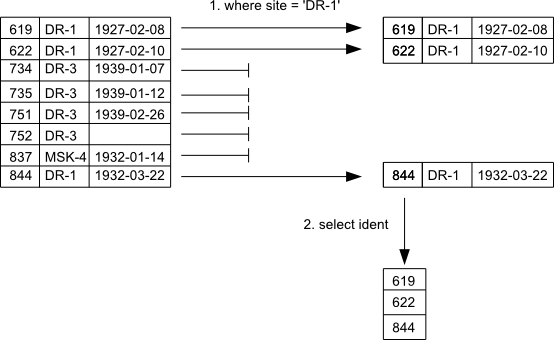
\includegraphics{novice/sql/img/sql-filter.png}

We can use many other Boolean operators to filter our data. For example,
we can ask for all information from the DR-1 site collected since 1930:

\begin{verbatim}
select * from Visited where (site='DR-1') and (dated>='1930-00-00');
\end{verbatim}

\begin{tabular}{lll}
844 & DR-1 & 1932-03-22 \\
\end{tabular}

(The parentheses around the individual tests aren't strictly required,
but they help make the query easier to read.)

\begin{swcbox}{Handling Dates}

Most database managers have a special data type for dates. In fact, many
have two: one for dates, such as ``May 31, 1971'', and one for
durations, such as ``31 days''. SQLite doesn't: instead, it stores dates
as either text (in the ISO-8601 standard format ``YYYY-MM-DD
HH:MM:SS.SSSS''), real numbers (the number of days since November 24,
4714 BCE), or integers (the number of seconds since midnight, January 1,
1970). If this sounds complicated, it is, but not nearly as complicated
as figuring out
\urlfoot{http://en.wikipedia.org/wiki/Swedish\_calendar}{historical dates in
Sweden}.

\end{swcbox}

If we want to find out what measurements were taken by either Lake or
Roerich, we can combine the tests on their names using \texttt{or}:

\begin{verbatim}
select * from Survey where person='lake' or person='roe';
\end{verbatim}

\begin{tabular}{llll}
734 & lake & sal & 0.05 \\
751 & lake & sal & 0.1 \\
752 & lake & rad & 2.19 \\
752 & lake & sal & 0.09 \\
752 & lake & temp & -16.0 \\
752 & roe & sal & 41.6 \\
837 & lake & rad & 1.46 \\
837 & lake & sal & 0.21 \\
837 & roe & sal & 22.5 \\
844 & roe & rad & 11.25 \\
\end{tabular}

Alternatively, we can use \texttt{in} to see if a value is in a specific
set:

\begin{verbatim}
select * from Survey where person in ('lake', 'roe');
\end{verbatim}

\begin{tabular}{llll}
734 & lake & sal & 0.05 \\
751 & lake & sal & 0.1 \\
752 & lake & rad & 2.19 \\
752 & lake & sal & 0.09 \\
752 & lake & temp & -16.0 \\
752 & roe & sal & 41.6 \\
837 & lake & rad & 1.46 \\
837 & lake & sal & 0.21 \\
837 & roe & sal & 22.5 \\
844 & roe & rad & 11.25 \\
\end{tabular}

We can combine \texttt{and} with \texttt{or}, but we need to be careful
about which operator is executed first. If we \emph{don't} use
parentheses, we get this:

\begin{verbatim}
select * from Survey where quant='sal' and person='lake' or person='roe';
\end{verbatim}

\begin{tabular}{llll}
734 & lake & sal & 0.05 \\
751 & lake & sal & 0.1 \\
752 & lake & sal & 0.09 \\
752 & roe & sal & 41.6 \\
837 & lake & sal & 0.21 \\
837 & roe & sal & 22.5 \\
844 & roe & rad & 11.25 \\
\end{tabular}

which is salinity measurements by Lake, and \emph{any} measurement by
Roerich. We probably want this instead:

\begin{verbatim}
select * from Survey where quant='sal' and (person='lake' or person='roe');
\end{verbatim}

\begin{tabular}{llll}
734 & lake & sal & 0.05 \\
751 & lake & sal & 0.1 \\
752 & lake & sal & 0.09 \\
752 & roe & sal & 41.6 \\
837 & lake & sal & 0.21 \\
837 & roe & sal & 22.5 \\
\end{tabular}

Finally, we can use \texttt{distinct} with \texttt{where} to give a
second level of filtering:

\begin{verbatim}
select distinct person, quant from Survey where person='lake' or person='roe';
\end{verbatim}

\begin{tabular}{ll}
lake & sal \\
lake & rad \\
lake & temp \\
roe & sal \\
roe & rad \\
\end{tabular}

But remember: \texttt{distinct} is applied to the values displayed in
the chosen columns, not to the entire rows as they are being processed.

\begin{swcbox}{Growing Queries}

What we have just done is how most people ``grow'' their SQL queries. We
started with something simple that did part of what we wanted, then
added more clauses one by one, testing their effects as we went. This is
a good strategy---in fact, for complex queries it's often the
\emph{only} strategy---but it depends on quick turnaround, and on us
recognizing the right answer when we get it.

The best way to achieve quick turnaround is often to put a subset of
data in a temporary database and run our queries against that, or to
fill a small database with synthesized records. For example, instead of
trying our queries against an actual database of 20 million Australians,
we could run it against a sample of ten thousand, or write a small
program to generate ten thousand random (but plausible) records and use
that.

\end{swcbox}

\begin{challenge}
  Suppose we want to select all sites that lie more than 30° from the
  poles. Our first query is:

\begin{verbatim}
select * from Site where (lat > -60) or (lat < 60);
\end{verbatim}

  Explain why this is wrong, and rewrite the query so that it is
  correct.
\end{challenge}

\begin{challenge}
  Normalized salinity readings are supposed to be between 0.0 and 1.0.
  Write a query that selects all records from \texttt{Survey} with
  salinity values outside this range.
\end{challenge}

\begin{challenge}
  The SQL test \texttt{*column-name* like *pattern*} is true if the
  value in the named column matches the pattern given; the character
  `\%' can be used any number of times in the pattern to mean ``match
  zero or more characters''.

  \begin{tabular}{ll}
  \hline\noalign{\medskip}
  Expression & Value
  \\\noalign{\medskip}
  \hline\noalign{\medskip}
  \texttt{'a' like 'a'} & True
  \\\noalign{\medskip}
  \texttt{'a' like '\%a'} & True
  \\\noalign{\medskip}
  \texttt{'b' like '\%a'} & False
  \\\noalign{\medskip}
  \texttt{'alpha' like 'a\%'} & True
  \\\noalign{\medskip}
  \texttt{'alpha' like 'a\%p\%'} & True
  \\\noalign{\medskip}
  \hline
  \end{tabular}

  The expression \texttt{*column-name* not like *pattern*} inverts the
  test. Using \texttt{like}, write a query that finds all the records in
  \texttt{Visited} that \emph{aren't} from sites labelled
  `DR-something'.
\end{challenge}

\begin{keypoints}
\begin{swcitemize}
\item
  Use \texttt{where} to filter records according to Boolean conditions.
\item
  Filtering is done on whole records, so conditions can use fields that
  are not actually displayed.
\end{swcitemize}
\end{keypoints}

\section{Calculating New Values}

\begin{objectives}
\begin{swcitemize}
\item
  Write queries that calculate new values for each selected record.
\end{swcitemize}
\end{objectives}

After carefully re-reading the expedition logs, we realize that the
radiation measurements they report may need to be corrected upward by
5\%. Rather than modifying the stored data, we can do this calculation
on the fly as part of our query:

\begin{verbatim}
%load_ext sqlitemagic
\end{verbatim}

\begin{verbatim}
select 1.05 * reading from Survey where quant='rad';
\end{verbatim}

\begin{tabular}{l}
10.311 \\
8.19 \\
8.8305 \\
7.581 \\
4.5675 \\
2.2995 \\
1.533 \\
11.8125 \\
\end{tabular}

When we run the query, the expression \texttt{1.05 * reading} is
evaluated for each row. Expressions can use any of the fields, all of
usual arithmetic operators, and a variety of common functions. (Exactly
which ones depends on which database manager is being used.) For
example, we can convert temperature readings from Fahrenheit to Celsius
and round to two decimal places:

\begin{verbatim}
select taken, round(5*(reading-32)/9, 2) from Survey where quant='temp';
\end{verbatim}

\begin{tabular}{ll}
734 & -29.72 \\
735 & -32.22 \\
751 & -28.06 \\
752 & -26.67 \\
\end{tabular}

We can also combine values from different fields, for example by using
the string concatenation operator \texttt{\textbar{}\textbar{}}:

\begin{verbatim}
select personal || ' ' || family from Person;
\end{verbatim}

\begin{tabular}{l}
William Dyer \\
Frank Pabodie \\
Anderson Lake \\
Valentina Roerich \\
Frank Danforth \\
\end{tabular}

\begin{swcbox}{What's in a Name?}

It may seem strange to use \texttt{personal} and \texttt{family} as
field names instead of \texttt{first} and \texttt{last}, but it's a
necessary first step toward handling cultural differences. For example,
consider the following rules:

\begin{tabular}{lll}
\hline\noalign{\medskip}
Full Name & Alphabetized Under & Reason
\\\noalign{\medskip}
\hline\noalign{\medskip}
Liu Xiaobo & Liu & Chinese family names come first
\\\noalign{\medskip}
Leonardo da Vinci & Leonardo & ``da Vinci'' just means ``from Vinci''
\\\noalign{\medskip}
Catherine de Medici & Medici & family name
\\\noalign{\medskip}
Jean de La Fontaine & La Fontaine & family name is ``La Fontaine''
\\\noalign{\medskip}
Juan Ponce de Leon & Ponce de Leon & full family name is ``Ponce de
Leon''
\\\noalign{\medskip}
Gabriel Garcia Marquez & Garcia Marquez & double-barrelled Spanish
surnames
\\\noalign{\medskip}
Wernher von Braun & von \emph{or} Braun & depending on whether he was in
Germany or the US
\\\noalign{\medskip}
Elizabeth Alexandra May Windsor & Elizabeth & monarchs alphabetize by
the name under which they reigned
\\\noalign{\medskip}
Thomas a Beckett & Thomas & and saints according to the names by which
they were canonized
\\\noalign{\medskip}
\hline
\end{tabular}

Clearly, even a two-part division into ``personal'' and ``family'' isn't
enough\ldots{}

\end{swcbox}

\begin{challenge}
  After further reading, we realize that Valentina Roerich was reporting
  salinity as percentages. Write a query that returns all of her
  salinity measurements from the \texttt{Survey} table with the values
  divided by 100.
\end{challenge}

\begin{challenge}
  The \texttt{union} operator combines the results of two queries:
\begin{verbatim}
select * from Person where ident='dyer' union select * from Person where ident='roe';
\end{verbatim}

\begin{tabular}{lll}
dyer & William & Dyer \\
roe & Valentina & Roerich \\
\end{tabular}

Use \texttt{union} to create a consolidated list of salinity
measurements in which Roerich's, and only Roerich's, have been corrected
as described in the previous challenge. The output should be something
like:

\begin{tabular}{ll}
619 & 0.13 \\
622 & 0.09 \\
734 & 0.05 \\
751 & 0.1 \\
752 & 0.09 \\
752 & 0.416 \\
837 & 0.21 \\
837 & 0.225 \\
\end{tabular}
\end{challenge}

\begin{challenge}
  The site identifiers in the \texttt{Visited} table have two parts
  separated by a `-':

\begin{verbatim}
select distinct site from Visited;
\end{verbatim}

\begin{tabular}{l}
DR-1 \\
DR-3 \\
MSK-4 \\
\end{tabular}

Some major site identifiers are two letters long and some are three. The
``in string'' function \texttt{instr(X, Y)} returns the 1-based index of
the first occurrence of string Y in string X, or 0 if Y does not exist
in X. The substring function \texttt{substr(X, I)} returns the substring
of X starting at index I. Use these two functions to produce a list of
unique major site identifiers. (For this data, the list should contain
only ``DR'' and ``MSK'').
\end{challenge}

\begin{keypoints}
\begin{swcitemize}
\item
  SQL can perform calculations using the values in a record as part of a
  query.
\end{swcitemize}
\end{keypoints}

\section{Missing Data}

\begin{objectives}
\begin{swcitemize}
\item
  Explain how databases represent missing information.
\item
  Explain the three-valued logic databases use when manipulating missing
  information.
\item
  Write queries that handle missing information correctly.
\end{swcitemize}
\end{objectives}

Real-world data is never complete---there are always holes. Databases
represent these holes using special value called \texttt{null}.
\texttt{null} is not zero, \texttt{False}, or the empty string; it is a
one-of-a-kind value that means ``nothing here''. Dealing with
\texttt{null} requires a few special tricks and some careful thinking.

To start, let's have a look at the \texttt{Visited} table. There are
eight records, but \#752 doesn't have a date---or rather, its date is
null:

\begin{verbatim}
%load_ext sqlitemagic
\end{verbatim}

\begin{verbatim}
select * from Visited;
\end{verbatim}

% FIXME: look for 'None' in tables
\begin{tabular}{lll}
619 & DR-1 & 1927-02-08 \\
622 & DR-1 & 1927-02-10 \\
734 & DR-3 & 1939-01-07 \\
735 & DR-3 & 1930-01-12 \\
751 & DR-3 & 1930-02-26 \\
752 & DR-3 & None \\
837 & MSK-4 & 1932-01-14 \\
844 & DR-1 & 1932-03-22 \\
\end{tabular}

Null doesn't behave like other values. If we select the records that
come before 1930:

\begin{verbatim}
select * from Visited where dated<'1930-00-00';
\end{verbatim}

\begin{tabular}{lll}
619 & DR-1 & 1927-02-08 \\
622 & DR-1 & 1927-02-10 \\
\end{tabular}

we get two results, and if we select the ones that come during or after
1930:

\begin{verbatim}
select * from Visited where dated>='1930-00-00';
\end{verbatim}

\begin{tabular}{lll}
734 & DR-3 & 1939-01-07 \\
735 & DR-3 & 1930-01-12 \\
751 & DR-3 & 1930-02-26 \\
837 & MSK-4 & 1932-01-14 \\
844 & DR-1 & 1932-03-22 \\
\end{tabular}

we get five, but record \#752 isn't in either set of results. The reason
is that \texttt{null\textless{}'1930-00-00'} is neither true nor false:
null means, ``We don't know,'' and if we don't know the value on the
left side of a comparison, we don't know whether the comparison is true
or false. Since databases represent ``don't know'' as null, the value of
\texttt{null\textless{}'1930-00-00'} is actually \texttt{null}.
\texttt{null\textgreater{}='1930-00-00'} is also null because we can't
answer to that question either. And since the only records kept by a
\texttt{where} are those for which the test is true, record \#752 isn't
included in either set of results.

Comparisons aren't the only operations that behave this way with nulls.
\texttt{1+null} is \texttt{null}, \texttt{5*null} is \texttt{null},
\texttt{log(null)} is \texttt{null}, and so on. In particular, comparing
things to null with = and != produces null:

\begin{verbatim}
select * from Visited where dated=NULL;
\end{verbatim}

% FIXME: empty table

\begin{verbatim}
select * from Visited where dated!=NULL;
\end{verbatim}

% FIXME: empty table

To check whether a value is \texttt{null} or not, we must use a special
test \texttt{is null}:

\begin{verbatim}
select * from Visited where dated is NULL;
\end{verbatim}

\begin{tabular}{lll}
752 & DR-3 & None \\
\end{tabular}

or its inverse \texttt{is not null}:

\begin{verbatim}
select * from Visited where dated is not NULL;
\end{verbatim}

\begin{tabular}{lll}
619 & DR-1 & 1927-02-08 \\
622 & DR-1 & 1927-02-10 \\
734 & DR-3 & 1939-01-07 \\
735 & DR-3 & 1930-01-12 \\
751 & DR-3 & 1930-02-26 \\
837 & MSK-4 & 1932-01-14 \\
844 & DR-1 & 1932-03-22 \\
\end{tabular}

Null values cause headaches wherever they appear. For example, suppose
we want to find all the salinity measurements that weren't taken by
Dyer. It's natural to write the query like this:

\begin{verbatim}
select * from Survey where quant='sal' and person!='lake';
\end{verbatim}

\begin{tabular}{llll}
619 & dyer & sal & 0.13 \\
622 & dyer & sal & 0.09 \\
752 & roe & sal & 41.6 \\
837 & roe & sal & 22.5 \\
\end{tabular}

but this query filters omits the records where we don't know who took
the measurement. Once again, the reason is that when \texttt{person} is
\texttt{null}, the \texttt{!=} comparison produces \texttt{null}, so the
record isn't kept in our results. If we want to keep these records we
need to add an explicit check:

\begin{verbatim}
select * from Survey where quant='sal' and (person!='lake' or person is null);
\end{verbatim}

\begin{tabular}{llll}
619 & dyer & sal & 0.13 \\
622 & dyer & sal & 0.09 \\
735 & None & sal & 0.06 \\
752 & roe & sal & 41.6 \\
837 & roe & sal & 22.5 \\
\end{tabular}

We still have to decide whether this is the right thing to do or not. If
we want to be absolutely sure that we aren't including any measurements
by Lake in our results, we need to exclude all the records for which we
don't know who did the work.

\begin{challenge}
  Write a query that sorts the records in \texttt{Visited} by date,
  omitting entries for which the date is not known (i.e., is null).
\end{challenge}

\begin{challenge}
  What do you expect the query:

\begin{verbatim}
select * from Visited where dated in ('1927-02-08', null);
\end{verbatim}

  to produce? What does it actually produce?
\end{challenge}

\begin{challenge}
  Some database designers prefer to use a
  \gl{sentinel value}{g:sentinel-value} to mark missing data
  rather than \texttt{null}. For example, they will use the date
  ``0000-00-00'' to mark a missing date, or -1.0 to mark a missing
  salinity or radiation reading (since actual readings cannot be
  negative). What does this simplify? What burdens or risks does it
  introduce?
\end{challenge}

\begin{keypoints}
\begin{swcitemize}
\item
  Databases use \texttt{null} to represent missing information.
\item
  Any arithmetic or Boolean operation involving \texttt{null} produces
  \texttt{null} as a result.
\item
  The only operators that can safely be used with \texttt{null} are
  \texttt{is null} and \texttt{is not null}.
\end{swcitemize}
\end{keypoints}

\section{Aggregation}

\begin{objectives}
\begin{swcitemize}
\item
  Define ``aggregation'' and give examples of its use.
\item
  Write queries that compute aggregated values.
\item
  Trace the execution of a query that performs aggregation.
\item
  Explain how missing data is handled during aggregation.
\end{swcitemize}
\end{objectives}

We now want to calculate ranges and averages for our data. We know how
to select all of the dates from the \texttt{Visited} table:

\begin{verbatim}
%load_ext sqlitemagic
\end{verbatim}

\begin{verbatim}
select dated from Visited;
\end{verbatim}

\begin{tabular}{l}
1927-02-08 \\
1927-02-10 \\
1939-01-07 \\
1930-01-12 \\
1930-02-26 \\
None \\
1932-01-14 \\
1932-03-22 \\
\end{tabular}

but to combine them, wee must use an
\gl{aggregation function}{g:aggregation-function} such as
\texttt{min} or \texttt{max}. Each of these functions takes a set of
records as input, and produces a single record as output:

\begin{verbatim}
select min(dated) from Visited;
\end{verbatim}

\begin{tabular}{l}
1927-02-08 \\
\end{tabular}

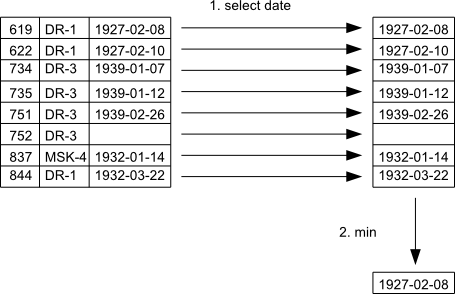
\includegraphics{novice/sql/img/sql-aggregation.png}

\begin{verbatim}
select max(dated) from Visited;
\end{verbatim}

\begin{tabular}{l}
1939-01-07 \\
\end{tabular}

\texttt{min} and \texttt{max} are just two of the aggregation functions
built into SQL. Three others are \texttt{avg}, \texttt{count}, and
\texttt{sum}:

\begin{verbatim}
select avg(reading) from Survey where quant='sal';
\end{verbatim}

\begin{tabular}{l}
7.20333333333 \\
\end{tabular}

\begin{verbatim}
select count(reading) from Survey where quant='sal';
\end{verbatim}

\begin{tabular}{l}
9 \\
\end{tabular}

\begin{verbatim}
select sum(reading) from Survey where quant='sal';
\end{verbatim}

\begin{tabular}{l}
64.83 \\
\end{tabular}

We used \texttt{count(reading)} here, but we could just as easily have
counted \texttt{quant} or any other field in the table, or even used
\texttt{count(*)}, since the function doesn't care about the values
themselves, just how many values there are.

SQL lets us do several aggregations at once. We can, for example, find
the range of sensible salinity measurements:

\begin{verbatim}
select min(reading), max(reading) from Survey where quant='sal' and reading<=1.0;
\end{verbatim}

\begin{tabular}{ll}
0.05 & 0.21 \\
\end{tabular}

We can also combine aggregated results with raw results, although the
output might surprise you:

\begin{verbatim}
select person, count(*) from Survey where quant='sal' and reading<=1.0;
\end{verbatim}

\begin{tabular}{ll}
lake & 7 \\
\end{tabular}

Why does Lake's name appear rather than Roerich's or Dyer's? The answer
is that when it has to aggregate a field, but isn't told how to, the
database manager chooses an actual value from the input set. It might
use the first one processed, the last one, or something else entirely.

Another important fact is that when there are no values to aggregate,
aggregation's result is ``don't know'' rather than zero or some other
arbitrary value:

\begin{verbatim}
select person, max(reading), sum(reading) from Survey where quant='missing';
\end{verbatim}

\begin{tabular}{lll} % FIXME: nulls in table
None & None & None \\
\end{tabular}

One final important feature of aggregation functions is that they are
inconsistent with the rest of SQL in a very useful way. If we add two
values, and one of them is null, the result is null. By extension, if we
use \texttt{sum} to add all the values in a set, and any of those values
are null, the result should also be null. It's much more useful, though,
for aggregation functions to ignore null values and only combine those
that are non-null. This behavior lets us write our queries as:

\begin{verbatim}
select min(dated) from Visited;
\end{verbatim}

\begin{tabular}{l}
1927-02-08 \\
\end{tabular}

instead of always having to filter explicitly:

\begin{verbatim}
select min(dated) from Visited where dated is not null;
\end{verbatim}

\begin{tabular}{l}
1927-02-08 \\
\end{tabular}

Aggregating all records at once doesn't always make sense. For example,
suppose Gina suspects that there is a systematic bias in her data, and
that some scientists' radiation readings are higher than others. We know
that this doesn't work:

\begin{verbatim}
select person, count(reading), round(avg(reading), 2)
from  Survey
where quant='rad';
\end{verbatim}

\begin{tabular}{lll}
roe & 8 & 6.56 \\
\end{tabular}

because the database manager selects a single arbitrary scientist's name
rather than aggregating separately for each scientist. Since there are
only five scientists, she could write five queries of the form:

\begin{verbatim}
select person, count(reading), round(avg(reading), 2)
from  Survey
where quant='rad'
and   person='dyer';
\end{verbatim}

\begin{tabular}{lll}
dyer & 2 & 8.81 \\
\end{tabular}

but this would be tedious, and if she ever had a data set with fifty or
five hundred scientists, the chances of her getting all of those queries
right is small.

What we need to do is tell the database manager to aggregate the hours
for each scientist separately using a \texttt{group by} clause:

\begin{verbatim}
select   person, count(reading), round(avg(reading), 2)
from     Survey
where    quant='rad'
group by person;
\end{verbatim}

\begin{tabular}{lll}
dyer & 2 & 8.81 \\
lake & 2 & 1.82 \\
pb & 3 & 6.66 \\
roe & 1 & 11.25 \\
\end{tabular}

\texttt{group by} does exactly what its name implies: groups all the
records with the same value for the specified field together so that
aggregation can process each batch separately. Since all the records in
each batch have the same value for \texttt{person}, it no longer matters
that the database manager is picking an arbitrary one to display
alongside the aggregated \texttt{reading} values.

Just as we can sort by multiple criteria at once, we can also group by
multiple criteria. To get the average reading by scientist and quantity
measured, for example, we just add another field to the
\texttt{group by} clause:

\begin{verbatim}
select   person, quant, count(reading), round(avg(reading), 2)
from     Survey
group by person, quant;
\end{verbatim}

\begin{tabular}{llll}
None & sal & 1 & 0.06 \\
None & temp & 1 & -26.0 \\
dyer & rad & 2 & 8.81 \\
dyer & sal & 2 & 0.11 \\
lake & rad & 2 & 1.82 \\
lake & sal & 4 & 0.11 \\
lake & temp & 1 & -16.0 \\
pb & rad & 3 & 6.66 \\
pb & temp & 2 & -20.0 \\
roe & rad & 1 & 11.25 \\
roe & sal & 2 & 32.05 \\
\end{tabular}

Note that we have added \texttt{person} to the list of fields displayed,
since the results wouldn't make much sense otherwise.

Let's go one step further and remove all the entries where we don't know
who took the measurement:

\begin{verbatim}
select   person, quant, count(reading), round(avg(reading), 2)
from     Survey
where    person is not null
group by person, quant
order by person, quant;
\end{verbatim}

\begin{tabular}{llll}
dyer & rad & 2 & 8.81 \\
dyer & sal & 2 & 0.11 \\
lake & rad & 2 & 1.82 \\
lake & sal & 4 & 0.11 \\
lake & temp & 1 & -16.0 \\
pb & rad & 3 & 6.66 \\
pb & temp & 2 & -20.0 \\
roe & rad & 1 & 11.25 \\
roe & sal & 2 & 32.05 \\
\end{tabular}

Looking more closely, this query:

\begin{swcenumerate}
\item
  selected records from the \texttt{Survey} table where the
  \texttt{person} field was not null;
\item
  grouped those records into subsets so that the \texttt{person} and
  \texttt{quant} values in each subset were the same;
\item
  ordered those subsets first by \texttt{person}, and then within each
  sub-group by \texttt{quant}; and
\item
  counted the number of records in each subset, calculated the average
  \texttt{reading} in each, and chose a \texttt{person} and
  \texttt{quant} value from each (it doesn't matter which ones, since
  they're all equal).
\end{swcenumerate}

\begin{challenge}
  How many temperature readings did Frank Pabodie record, and what was
  their average value?
\end{challenge}

\begin{challenge}
  The average of a set of values is the sum of the values divided by the
  number of values. Does this mean that the \texttt{avg} function
  returns 2.0 or 3.0 when given the values 1.0, \texttt{null}, and 5.0?
\end{challenge}

\begin{challenge}
  We want to calculate the difference between each individual radiation
  reading and the average of all the radiation readings. We write the
  query:

\begin{verbatim}
select reading - avg(reading) from Survey where quant='rad';
\end{verbatim}

  What does this actually produce, and why?
\end{challenge}

\begin{challenge}
  The function \texttt{group\_concat(field, separator)} concatenates all
  the values in a field using the specified separator character (or `,'
  if the separator isn't specified). Use this to produce a one-line list
  of scientists' names, such as:

\begin{verbatim}
William Dyer, Frank Pabodie, Anderson Lake, Valentina Roerich, Frank Danforth
\end{verbatim}

  Can you find a way to order the list by surname?
\end{challenge}

\begin{keypoints}
\begin{swcitemize}
\item
  An aggregation function combines many values to produce a single new
  value.
\item
  Aggregation functions ignore \texttt{null} values.
\item
  Aggregation happens after filtering.
\end{swcitemize}
\end{keypoints}

\section{Combining Data}

\begin{objectives}
\begin{swcitemize}
\item
  Explain the operation of a query that joins two tables.
\item
  Explain how to restrict the output of a query containing a join to
  only include meaningful combinations of values.
\item
  Write queries that join tables on equal keys.
\item
  Explain what primary and foreign keys are, and why they are useful.
\item
  Explain what atomic values are, and why database fields should only
  contain atomic values.
\end{swcitemize}
\end{objectives}

In order to submit her data to a web site that aggregates historical
meteorological data, Gina needs to format it as latitude, longitude,
date, quantity, and reading. However, her latitudes and longitudes are
in the \texttt{Site} table, while the dates of measurements are in the
\texttt{Visited} table and the readings themselves are in the
\texttt{Survey} table. She needs to combine these tables somehow.

The SQL command to do this is \texttt{join}. To see how it works, let's
start by joining the \texttt{Site} and \texttt{Visited} tables:

\begin{verbatim}
%load_ext sqlitemagic
\end{verbatim}

\begin{verbatim}
select * from Site join Visited;
\end{verbatim}

\begin{tabular}{llllll}
DR-1 & -49.85 & -128.57 & 619 & DR-1 & 1927-02-08 \\
DR-1 & -49.85 & -128.57 & 622 & DR-1 & 1927-02-10 \\
DR-1 & -49.85 & -128.57 & 734 & DR-3 & 1939-01-07 \\
DR-1 & -49.85 & -128.57 & 735 & DR-3 & 1930-01-12 \\
DR-1 & -49.85 & -128.57 & 751 & DR-3 & 1930-02-26 \\
DR-1 & -49.85 & -128.57 & 752 & DR-3 & None \\
DR-1 & -49.85 & -128.57 & 837 & MSK-4 & 1932-01-14 \\
DR-1 & -49.85 & -128.57 & 844 & DR-1 & 1932-03-22 \\
DR-3 & -47.15 & -126.72 & 619 & DR-1 & 1927-02-08 \\
DR-3 & -47.15 & -126.72 & 622 & DR-1 & 1927-02-10 \\
DR-3 & -47.15 & -126.72 & 734 & DR-3 & 1939-01-07 \\
DR-3 & -47.15 & -126.72 & 735 & DR-3 & 1930-01-12 \\
DR-3 & -47.15 & -126.72 & 751 & DR-3 & 1930-02-26 \\
DR-3 & -47.15 & -126.72 & 752 & DR-3 & None \\
DR-3 & -47.15 & -126.72 & 837 & MSK-4 & 1932-01-14 \\
DR-3 & -47.15 & -126.72 & 844 & DR-1 & 1932-03-22 \\
MSK-4 & -48.87 & -123.4 & 619 & DR-1 & 1927-02-08 \\
MSK-4 & -48.87 & -123.4 & 622 & DR-1 & 1927-02-10 \\
MSK-4 & -48.87 & -123.4 & 734 & DR-3 & 1939-01-07 \\
MSK-4 & -48.87 & -123.4 & 735 & DR-3 & 1930-01-12 \\
MSK-4 & -48.87 & -123.4 & 751 & DR-3 & 1930-02-26 \\
MSK-4 & -48.87 & -123.4 & 752 & DR-3 & None \\
MSK-4 & -48.87 & -123.4 & 837 & MSK-4 & 1932-01-14 \\
MSK-4 & -48.87 & -123.4 & 844 & DR-1 & 1932-03-22 \\
\end{tabular}

\texttt{join} creates the \gl{cross product}{g:cross-product} of
two tables, i.e., it joins each record of one with each record of the
other to give all possible combinations. Since there are three records
in \texttt{Site} and eight in \texttt{Visited}, the join's output has 24
records. And since each table has three fields, the output has six
fields.

What the join \emph{hasn't} done is figure out if the records being
joined have anything to do with each other. It has no way of knowing
whether they do or not until we tell it how. To do that, we add a clause
specifying that we're only interested in combinations that have the same
site name:

\begin{verbatim}
select * from Site join Visited on Site.name=Visited.site;
\end{verbatim}

\begin{tabular}{llllll}
DR-1 & -49.85 & -128.57 & 619 & DR-1 & 1927-02-08 \\
DR-1 & -49.85 & -128.57 & 622 & DR-1 & 1927-02-10 \\
DR-1 & -49.85 & -128.57 & 844 & DR-1 & 1932-03-22 \\
DR-3 & -47.15 & -126.72 & 734 & DR-3 & 1939-01-07 \\
DR-3 & -47.15 & -126.72 & 735 & DR-3 & 1930-01-12 \\
DR-3 & -47.15 & -126.72 & 751 & DR-3 & 1930-02-26 \\
DR-3 & -47.15 & -126.72 & 752 & DR-3 & None \\
MSK-4 & -48.87 & -123.4 & 837 & MSK-4 & 1932-01-14 \\
\end{tabular}

\texttt{on} does the same job as \texttt{where}: it only keeps records
that pass some test. (The difference between the two is that \texttt{on}
filters records as they're being created, while \texttt{where} waits
until the join is done and then does the filtering.) Once we add this to
our query, the database manager throws away records that combined
information about two different sites, leaving us with just the ones we
want.

Notice that we used \texttt{table.field} to specify field names in the
output of the join. We do this because tables can have fields with the
same name, and we need to be specific which ones we're talking about.
For example, if we joined the \texttt{person} and \texttt{visited}
tables, the result would inherit a field called \texttt{ident} from each
of the original tables.

We can now use the same dotted notation to select the three columns we
actually want out of our join:

\begin{verbatim}
select Site.lat, Site.long, Visited.dated
from   Site join Visited
on     Site.name=Visited.site;
\end{verbatim}

\begin{tabular}{lll}
-49.85 & -128.57 & 1927-02-08 \\
-49.85 & -128.57 & 1927-02-10 \\
-49.85 & -128.57 & 1932-03-22 \\
-47.15 & -126.72 & None \\
-47.15 & -126.72 & 1930-01-12 \\
-47.15 & -126.72 & 1930-02-26 \\
-47.15 & -126.72 & 1939-01-07 \\
-48.87 & -123.4 & 1932-01-14 \\
\end{tabular}

If joining two tables is good, joining many tables must be better. In
fact, we can join any number of tables simply by adding more
\texttt{join} clauses to our query, and more \texttt{on} tests to filter
out combinations of records that don't make sense:

\begin{verbatim}
select Site.lat, Site.long, Visited.dated, Survey.quant, Survey.reading
from   Site join Visited join Survey
on     Site.name=Visited.site
and    Visited.ident=Survey.taken
and    Visited.dated is not null;
\end{verbatim}

\begin{tabular}{lllll}
-49.85 & -128.57 & 1927-02-08 & rad & 9.82 \\
-49.85 & -128.57 & 1927-02-08 & sal & 0.13 \\
-49.85 & -128.57 & 1927-02-10 & rad & 7.8 \\
-49.85 & -128.57 & 1927-02-10 & sal & 0.09 \\
-47.15 & -126.72 & 1939-01-07 & rad & 8.41 \\
-47.15 & -126.72 & 1939-01-07 & sal & 0.05 \\
-47.15 & -126.72 & 1939-01-07 & temp & -21.5 \\
-47.15 & -126.72 & 1930-01-12 & rad & 7.22 \\
-47.15 & -126.72 & 1930-01-12 & sal & 0.06 \\
-47.15 & -126.72 & 1930-01-12 & temp & -26.0 \\
-47.15 & -126.72 & 1930-02-26 & rad & 4.35 \\
-47.15 & -126.72 & 1930-02-26 & sal & 0.1 \\
-47.15 & -126.72 & 1930-02-26 & temp & -18.5 \\
-48.87 & -123.4 & 1932-01-14 & rad & 1.46 \\
-48.87 & -123.4 & 1932-01-14 & sal & 0.21 \\
-48.87 & -123.4 & 1932-01-14 & sal & 22.5 \\
-49.85 & -128.57 & 1932-03-22 & rad & 11.25 \\
\end{tabular}

We can tell which records from \texttt{Site}, \texttt{Visited}, and
\texttt{Survey} correspond with each other because those tables contain
\gl{primary keys}{g:primary-key} and
\gl{foreign keys}{g:foreign-key}. A primary key is a value, or
combination of values, that uniquely identifies each record in a table.
A foreign key is a value (or combination of values) from one table that
identifies a unique record in another table. Another way of saying this
is that a foreign key is the primary key of one table that appears in
some other table. In our database, \texttt{Person.ident} is the primary
key in the \texttt{Person} table, while \texttt{Survey.person} is a
foreign key relating the \texttt{Survey} table's entries to entries in
\texttt{Person}.

Most database designers believe that every table should have a
well-defined primary key. They also believe that this key should be
separate from the data itself, so that if we ever need to change the
data, we only need to make one change in one place. One easy way to do
this is to create an arbitrary, unique ID for each record as we add it
to the database. This is actually very common: those IDs have names like
``student numbers'' and ``patient numbers'', and they almost always turn
out to have originally been a unique record identifier in some database
system or other. As the query below demonstrates, SQLite automatically
numbers records as they're added to tables, and we can use those record
numbers in queries:

\begin{verbatim}
select rowid, * from Person;
\end{verbatim}

\begin{tabular}{llll}
1 & dyer & William & Dyer \\
2 & pb & Frank & Pabodie \\
3 & lake & Anderson & Lake \\
4 & roe & Valentina & Roerich \\
5 & danforth & Frank & Danforth \\
\end{tabular}

\subsection{Data Hygiene}

Now that we have seen how joins work, we can see why the relational
model is so useful and how best to use it. The first rule is that every
value should be \gl{atomic}{g:atomic-value}, i.e., not contain
parts that we might want to work with separately. We store personal and
family names in separate columns instead of putting the entire name in
one column so that we don't have to use substring operations to get the
name's components. More importantly, we store the two parts of the name
separately because splitting on spaces is unreliable: just think of a
name like ``Eloise St. Cyr'' or ``Jan Mikkel Steubart''.

The second rule is that every record should have a unique primary key.
This can be a serial number that has no intrinsic meaning, one of the
values in the record (like the \texttt{ident} field in the
\texttt{Person} table), or even a combination of values: the triple
\texttt{(taken, person, quant)} from the \texttt{Survey} table uniquely
identifies every measurement.

The third rule is that there should be no redundant information. For
example, we could get rid of the \texttt{Site} table and rewrite the
\texttt{Visited} table like this:

\begin{tabular}{llll}
619 & -49.85 & -128.57 & 1927-02-08 \\
622 & -49.85 & -128.57 & 1927-02-10 \\
734 & -47.15 & -126.72 & 1939-01-07 \\
735 & -47.15 & -126.72 & 1930-01-12 \\
751 & -47.15 & -126.72 & 1930-02-26 \\
752 & -47.15 & -126.72 & null \\
837 & -48.87 & -123.40 & 1932-01-14 \\
844 & -49.85 & -128.57 & 1932-03-22 \\
\end{tabular}

In fact, we could use a single table that recorded all the information
about each reading in each row, just as a spreadsheet would. The problem
is that it's very hard to keep data organized this way consistent: if we
realize that the date of a particular visit to a particular site is
wrong, we have to change multiple records in the database. What's worse,
we may have to guess which records to change, since other sites may also
have been visited on that date.

The fourth rule is that the units for every value should be stored
explicitly. Our database doesn't do this, and that's a problem:
Roerich's salinity measurements are several orders of magnitude larger
than anyone else's, but we don't know if that means she was using parts
per million instead of parts per thousand, or whether there actually was
a saline anomaly at that site in 1932.

Stepping back, data and the tools used to store it have a symbiotic
relationship: we use tables and joins because it's efficient, provided
our data is organized a certain way, but organize our data that way
because we have tools to manipulate it efficiently if it's in a certain
form. As anthropologists say, the tool shapes the hand that shapes the
tool.

\begin{challenge}
  Write a query that lists all radiation readings from the DR-1 site.
\end{challenge}

\begin{challenge}
  Write a query that lists all sites visited by people named ``Frank''.
\end{challenge}

\begin{challenge}
  Describe in your own words what the following query produces:

\begin{verbatim}
select Site.name from Site join Visited
on Site.lat<-49.0 and Site.name=Visited.site and Visited.dated>='1932-00-00';
\end{verbatim}
\end{challenge}

\begin{keypoints}
\begin{swcitemize}
\item
  Every fact should be represented in a database exactly once.
\item
  A join produces all combinations of records from one table with
  records from another.
\item
  A primary key is a field (or set of fields) whose values uniquely
  identify the records in a table.
\item
  A foreign key is a field (or set of fields) in one table whose values
  are a primary key in another table.
\item
  We can eliminate meaningless combinations of records by matching
  primary keys and foreign keys between tables.
\item
  Keys should be atomic values to make joins simpler and more efficient.
\end{swcitemize}
\end{keypoints}

\section{Creating and Modifying Data}

\begin{objectives}
\begin{swcitemize}
\item
  Write queries that creates tables.
\item
  Write queries to insert, modify, and delete records.
\end{swcitemize}
\end{objectives}

So far we have only looked at how to get information out of a database,
both because that is more frequent than adding information, and because
most other operations only make sense once queries are understood. If we
want to create and modify data, we need to know two other pairs of
commands.

The first pair are \texttt{create table} and \texttt{drop table}. While
they are written as two words, they are actually single commands. The
first one creates a new table; its arguments are the names and types of
the table's columns. For example, the following statements create the
four tables in our survey database:

\begin{verbatim}
create table Person(ident text, personal text, family text);
create table Site(name text, lat real, long real);
create table Visited(ident integer, site text, dated text);
create table Survey(taken integer, person text, quant real, reading real);
\end{verbatim}

We can get rid of one of our tables using:

\begin{verbatim}
drop table Survey;
\end{verbatim}

Be very careful when doing this: most databases have some support for
undoing changes, but it's better not to have to rely on it.

Different database systems support different data types for table
columns, but most provide the following:

\begin{tabular}{ll}
\hline\noalign{\medskip}
integer & a signed integer
\\\noalign{\medskip}
real & a floating point number
\\\noalign{\medskip}
text & a character string
\\\noalign{\medskip}
blob & a ``binary large object'', such as an image
\\\noalign{\medskip}
\hline
\end{tabular}

Most databases also support Booleans and date/time values; SQLite uses
the integers 0 and 1 for the former, and represents the latter as
discussed \gl{earlier}{a:dates}. An increasing number of databases
also support geographic data types, such as latitude and longitude.
Keeping track of what particular systems do or do not offer, and what
names they give different data types, is an unending portability
headache.

When we create a table, we can specify several kinds of constraints on
its columns. For example, a better definition for the \texttt{Survey}
table would be:

\begin{verbatim}
create table Survey(
    taken   integer not null, -- where reading taken
    person  text,             -- may not know who took it
    quant   real not null,    -- the quantity measured
    reading real not null,    -- the actual reading
    primary key(taken, quant),
    foreign key(taken) references Visited(ident),
    foreign key(person) references Person(ident)
);
\end{verbatim}

Once again, exactly what constraints are avialable and what they're
called depends on which database manager we are using.

Once tables have been created, we can add and remove records using our
other pair of commands, \texttt{insert} and \texttt{delete}. The
simplest form of \texttt{insert} statement lists values in order:

\begin{verbatim}
insert into Site values('DR-1', -49.85, -128.57);
insert into Site values('DR-3', -47.15, -126.72);
insert into Site values('MSK-4', -48.87, -123.40);
\end{verbatim}

We can also insert values into one table directly from another:

\begin{verbatim}
create table JustLatLong(lat text, long text);
insert into JustLatLong select lat, long from site;
\end{verbatim}

Deleting records can be a bit trickier, because we have to ensure that
the database remains internally consistent. If all we care about is a
single table, we can use the \texttt{delete} command with a
\texttt{where} clause that matches the records we want to discard. For
example, once we realize that Frank Danforth didn't take any
measurements, we can remove him from the \texttt{Person} table like
this:

\begin{verbatim}
delete from Person where ident = "danforth";
\end{verbatim}

But what if we removed Anderson Lake instead? Our \texttt{Survey} table
would still contain seven records of measurements he'd taken, but that's
never supposed to happen: \texttt{Survey.person} is a foreign key into
the \texttt{Person} table, and all our queries assume there will be a
row in the latter matching every value in the former.

This problem is called \gl{referential
integrity}{g:referential-integrity}: we need to ensure that all references between tables can
always be resolved correctly. One way to do this is to delete all the
records that use \texttt{'lake'} as a foreign key before deleting the
record that uses it as a primary key. If our database manager supports
it, we can automate this using \gl{cascading
delete}{g:cascading-delete}. However, this technique is outside the scope of this chapter.

\begin{swcbox}{Mix and Match}

Many applications use a hybrid storage model instead of putting
everything into a database: the actual data (such as astronomical
images) is stored in files, while the database stores the files' names,
their modification dates, the region of the sky they cover, their
spectral characteristics, and so on. This is also how most music player
software is built: the database inside the application keeps track of
the MP3 files, but the files themselves live on disk.

\end{swcbox}

\begin{challenge}
  Write an SQL statement to replace all uses of \texttt{null} in
  \texttt{Survey.person} with the string \texttt{'unknown'}.
\end{challenge}

\begin{challenge}
  One of our colleagues has sent us a \gl{CSV}{g:csv} file
  containing temperature readings by Robert Olmstead, which is formatted
  like this:

\begin{verbatim}
Taken,Temp
619,-21.5
622,-15.5
\end{verbatim}

  Write a small Python program that reads this file in and prints out
  the SQL \texttt{insert} statements needed to add these records to the
  survey database. Note: you will need to add an entry for Olmstead to
  the \texttt{Person} table. If you are testing your program repeatedly,
  you may want to investigate SQL's \texttt{insert or replace} command.
\end{challenge}

\begin{challenge}
  SQLite has several administrative commands that aren't part of the SQL
  standard. One of them is \texttt{.dump}, which prints the SQL commands
  needed to re-create the database. Another is \texttt{.load}, which
  reads a file created by \texttt{.dump} and restores the database. A
  colleague of yours thinks that storing dump files (which are text) in
  version control is a good way to track and manage changes to the
  database. What are the pros and cons of this approach? (Hint: records
  aren't stored in any particular order.)
\end{challenge}

\begin{keypoints}
\begin{swcitemize}
\item
  Database tables are created using queries that specify their names and
  the names and properties of their fields.
\item
  Records can be inserted, updated, or deleted using queries.
\item
  It is simpler and safer to modify data when every record has a unique
  primary key.
\end{swcitemize}
\end{keypoints}

\section{Programming with Databases}

\begin{objectives}
\begin{swcitemize}
\item
  Write short programs that execute SQL queries.
\item
  Trace the execution of a program that contains an SQL query.
\item
  Explain why most database applications are written in a
  general-purpose language rather than in SQL.
\end{swcitemize}
\end{objectives}

To close, let's have a look at how to access a database from a
general-purpose programming language like Python. Other languages use
almost exactly the same model: library and function names may differ,
but the concepts are the same.

Here's a short Python program that selects latitudes and longitudes from
an SQLite database stored in a file called \texttt{survey.db}:

\begin{verbatim}
import sqlite3
connection = sqlite3.connect("survey.db")
cursor = connection.cursor()
cursor.execute("select site.lat, site.long from site;")
results = cursor.fetchall()
for r in results:
    print r
cursor.close()
connection.close()
\end{verbatim}

\begin{verbatim}
(-49.85, -128.57)
(-47.15, -126.72)
(-48.87, -123.4)
\end{verbatim}

The program starts by importing the \texttt{sqlite3} library. If we were
connecting to MySQL, DB2, or some other database, we would import a
different library, but all of them provide the same functions, so that
the rest of our program does not have to change (at least, not much) if
we switch from one database to another.

Line 2 establishes a connection to the database. Since we're using
SQLite, all we need to specify is the name of the database file. Other
systems may require us to provide a username and password as well. Line
3 then uses this connection to create a \gl{cursor}{g:cursor};
just like the cursor in an editor, its role is to keep track of where we
are in the database.

On line 4, we use that cursor to ask the database to execute a query for
us. The query is written in SQL, and passed to \texttt{cursor.execute}
as a string. It's our job to make sure that SQL is properly formatted;
if it isn't, or if something goes wrong when it is being executed, the
database will report an error.

The database returns the results of the query to us in response to the
\texttt{cursor.fetchall} call on line 5. This result is a list with one
entry for each record in the result set; if we loop over that list (line
6) and print those list entries (line 7), we can see that each one is a
tuple with one element for each field we asked for.

Finally, lines 8 and 9 close our cursor and our connection, since the
database can only keep a limited number of these open at one time. Since
establishing a connection takes time, though, we shouldn't open a
connection, do one operation, then close the connection, only to reopen
it a few microseconds later to do another operation. Instead, it's
normal to create one connection that stays open for the lifetime of the
program.

Queries in real applications will often depend on values provided by
users. For example, this function takes a user's ID as a parameter and
returns their name:

\begin{verbatim}
def get_name(database_file, person_ident):
    query = "select personal || ' ' || family from Person where ident='" + person_ident + "';"

    connection = sqlite3.connect(database_file)
    cursor = connection.cursor()
    cursor.execute(query)
    results = cursor.fetchall()
    cursor.close()
    connection.close()

    return results[0][0]

print "full name for dyer:", get_name('survey.db', 'dyer')
\end{verbatim}

\begin{verbatim}
full name for dyer: William Dyer
\end{verbatim}

We use string concatenation on the first line of this function to
construct a query containing the user ID we have been given. This seems
simple enough, but what happens if someone gives us this string as
input?

\begin{verbatim}
dyer'; drop table Survey; select '
\end{verbatim}

It looks like there's garbage after the name of the project, but it is
very carefully chosen garbage. If we insert this string into our query,
the result is:

\begin{verbatim}
select personal || ' ' || family from Person where ident='dyer'; drop tale Survey; select '';
\end{verbatim}

If we execute this, it will erase one of the tables in our database.

This is called an \gl{SQL injection
attack}{g:sql-injection-attack}, and it has been used to attack thousands of programs over the
years. In particular, many web sites that take data from users insert
values directly into queries without checking them carefully first.

Since a villain might try to smuggle commands into our queries in many
different ways, the safest way to deal with this threat is to replace
characters like quotes with their escaped equivalents, so that we can
safely put whatever the user gives us inside a string. We can do this by
using a \gl{prepared statement}{g:prepared-statement} instead of
formatting our statements as strings. Here's what our example program
looks like if we do this:

\begin{verbatim}
def get_name(database_file, person_ident):
    query = "select personal || ' ' || family from Person where ident=?;"

    connection = sqlite3.connect(database_file)
    cursor = connection.cursor()
    cursor.execute(query, [person_ident])
    results = cursor.fetchall()
    cursor.close()
    connection.close()

    return results[0][0]

print "full name for dyer:", get_name('survey.db', 'dyer')
\end{verbatim}

\begin{verbatim}
full name for dyer: William Dyer
\end{verbatim}

The key changes are in the query string and the \texttt{execute} call.
Instead of formatting the query ourselves, we put question marks in the
query template where we want to insert values. When we call
\texttt{execute}, we provide a list that contains as many values as
there are question marks in the query. The library matches values to
question marks in order, and translates any special characters in the
values into their escaped equivalents so that they are safe to use.

\begin{challenge}
  Write a Python program that creates a new database in a file called
  \texttt{original.db} containing a single table called
  \texttt{Pressure}, with a single field called \texttt{reading}, and
  inserts 100,000 random numbers between 10.0 and 25.0. How long does it
  take this program to run? How long does it take to run a program that
  simply writes those random numbers to a file?
\end{challenge}

\begin{challenge}
  Write a Python program that creates a new database called
  \texttt{backup.db} with the same structure as \texttt{original.db} and
  copies all the values greater than 20.0 from \texttt{original.db} to
  \texttt{backup.db}. Which is faster: filtering values in the query, or
  reading everything into memory and filtering in Python?
\end{challenge}

\begin{keypoints}
\begin{swcitemize}
\item
  We usually write database applications in a general-purpose language,
  and embed SQL queries in it.
\item
  To connect to a database, a program must use a library specific to
  that database manager.
\item
  A program may open one or more connections to a single database, and
  have one or more cursors active in each.
\item
  Programs can read query results in batches or all at once.
\end{swcitemize}
\end{keypoints}

\chapter{A Few Extras}\label{s:extras}

A few things come up in our classes that don't fit naturally into the
flow of our lessons. We have gathered several of them here.

\section{Branching in Git}

Here's where we are right now:

\begin{verbatim}
$ git log
\end{verbatim}

\begin{verbatim}
commit 005937fbe2a98fb83f0ade869025dc2636b4dad5
Author: Vlad Dracula <vlad@tran.sylvan.ia>
Date:   Thu Aug 22 10:14:07 2013 -0400

    Thoughts about the climate

commit 34961b159c27df3b475cfe4415d94a6d1fcd064d
Author: Vlad Dracula <vlad@tran.sylvan.ia>
Date:   Thu Aug 22 10:07:21 2013 -0400

    Concerns about Mars's moons on my furry friend

commit f22b25e3233b4645dabd0d81e651fe074bd8e73b
Author: Vlad Dracula <vlad@tran.sylvan.ia>
Date:   Thu Aug 22 09:51:46 2013 -0400

    Starting to think about Mars

$ cat mars.txt
Cold and dry, but everything is my favorite color
The two moons may be a problem for Wolfman
But the Mummy will appreciate the lack of humidity
\end{verbatim}

We can draw the history of the repository like this (we'll see in a
second why there's a box called \texttt{master}):

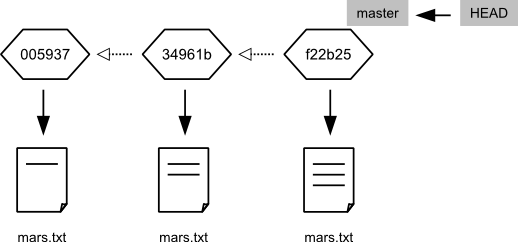
\includegraphics{novice/extras/img/git-branching-01.png}

Let's run this command:

\begin{verbatim}
$ git branch moons
\end{verbatim}

It appears to do nothing, but behind the scenes it has created a new
\gl{branch}{g:branch} called \texttt{moons}:

\begin{verbatim}
$ git branch
\end{verbatim}

\begin{verbatim}
* master
  moons
\end{verbatim}

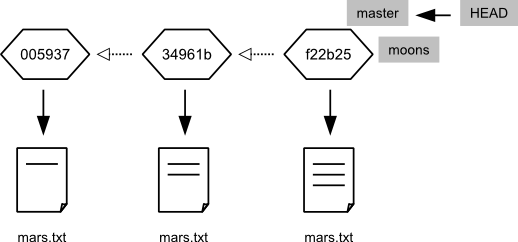
\includegraphics{novice/extras/img/git-branching-02.png}

Git is now maintaining two named bookmarks in our history:
\texttt{master}, which was created automatically when we set up the
repository, and \texttt{moons}, which we just made. They both point to
the same revision right now, but we can change that. Let's make
\texttt{moons} the active branch:

\begin{verbatim}
$ git checkout moons
\end{verbatim}

\begin{verbatim}
Switched to branch 'moons'
\end{verbatim}

\begin{verbatim}
$ git branch
\end{verbatim}

\begin{verbatim}
  master
* moons
\end{verbatim}

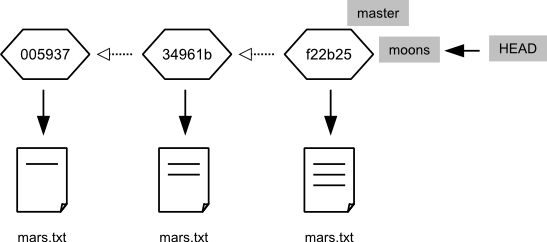
\includegraphics{novice/extras/img/git-branching-03.png}

Our file looks the same:

\begin{verbatim}
$ cat mars.txt
\end{verbatim}

\begin{verbatim}
Cold and dry, but everything is my favorite color
The two moons may be a problem for Wolfman
But the Mummy will appreciate the lack of humidity
\end{verbatim}

because it \emph{is} the same: Let's add another line to it:

\begin{verbatim}
$ echo "Maybe we should put the base on one of the moons instead?" >> mars.txt
\end{verbatim}

and add an entirely new file:

\begin{verbatim}
$ echo "Phobos is larger than Deimos" > moons.txt
$ ls
\end{verbatim}

\begin{verbatim}
mars.txt    moons.txt
\end{verbatim}

Git now tells us that we have one changed file and one new file:

\begin{verbatim}
$ git status
\end{verbatim}

\begin{verbatim}
# On branch moons
# Changes not staged for commit:
#   (use "git add <file>..." to update what will be committed)
#   (use "git checkout -- <file>..." to discard changes in working directory)
#
#    modified:   mars.txt
#
# Untracked files:
#   (use "git add <file>..." to include in what will be committed)
#
#    moons.txt
no changes added to commit (use "git add" and/or "git commit -a")
\end{verbatim}

Let's add and commit those changes (the \texttt{-A} flag to
\texttt{git commit} means ``add everything''):

\begin{verbatim}
$ git add -A
$ git status
\end{verbatim}

\begin{verbatim}
# On branch moons
# Changes to be committed:
#   (use "git reset HEAD <file>..." to unstage)
#
#    modified:   mars.txt
#    new file:   moons.txt
#
\end{verbatim}

\begin{verbatim}
$ git commit -m "Thinking about the moons"
\end{verbatim}

\begin{verbatim}
[moons 62e7791] Thinking about the moons
 2 files changed, 2 insertions(+)
 create mode 100644 moons.txt
\end{verbatim}

Our repository is now in the state shown below:

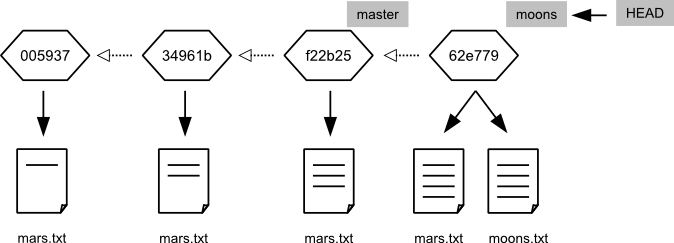
\includegraphics{novice/extras/img/git-branching-04.png}

The \texttt{moons} branch has advanced to record the changes we just
made, but \texttt{master} is still where it was. If we switch back to
\texttt{master}:

\begin{verbatim}
$ git checkout master
\end{verbatim}

our changes seem to disappear:

\begin{verbatim}
$ ls
\end{verbatim}

\begin{verbatim}
mars.txt
\end{verbatim}

\begin{verbatim}
$ cat mars.txt
\end{verbatim}

\begin{verbatim}
Cold and dry, but everything is my favorite color
The two moons may be a problem for Wolfman
But the Mummy will appreciate the lack of humidity
\end{verbatim}

They're still in the repository---they're just not in the revision that
\texttt{master} is currently pointing to. In essence, we've created a
parallel timeline that shares some history with the original one before
diverging.

Let's make some changes in the \texttt{master} branch to further
illustrate this point:

\begin{verbatim}
$ echo "Should we go with a classical name like Ares Base?" > names.txt
$ git status
\end{verbatim}

\begin{verbatim}
# On branch master
# Untracked files:
#   (use "git add <file>..." to include in what will be committed)
#
#    names.txt
nothing added to commit but untracked files present (use "git add" to track)
\end{verbatim}

\begin{verbatim}
$ git add names.txt
$ git commit -m "We will need a cool name for our secret base"
\end{verbatim}

\begin{verbatim}
[master dfcf908] We will need a cool name for our secret base
 1 file changed, 1 insertion(+)
 create mode 100644 names.txt
\end{verbatim}

Our repository is now in this state:

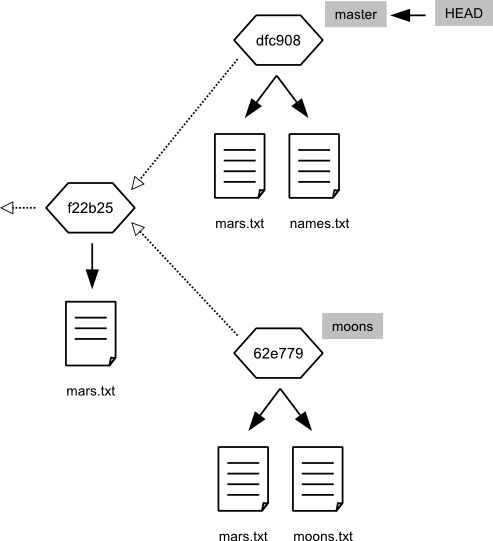
\includegraphics{novice/extras/img/git-branching-05.png}

\texttt{master} and \texttt{moons} have both moved on from their
original common state, but in different ways. They could continue
independent existence indefinitely, but at some point we'll probably
want to \gl{merge}{g:merge} our changes. Let's do that now:

\begin{verbatim}
$ git branch
\end{verbatim}

\begin{verbatim}
* master
  moons
\end{verbatim}

\begin{verbatim}
$ git merge moons
\end{verbatim}

When we run the \texttt{git merge} command, Git opens an editor to let
us write a log entry about what we're doing. The editor session
initially contains this:

\begin{verbatim}
Merge branch 'moons'

# Please enter a commit message to explain why this merge is necessary,
# especially if it merges an updated upstream into a topic branch.
#
# Lines starting with '#' will be ignored, and an empty message aborts
# the commit.
\end{verbatim}

If we notice that something is wrong and decide not to complete the
merge, we must delete everything in the file---Git interprets an empty
log message to mean, ``Don't proceed.'' Otherwise, everything that isn't
marked as a comment with \texttt{\#} will be saved to the log. In this
case, we'll stick with the default log message. When we save the file
and exit the editor, Git displays this:

\begin{verbatim}
Merge made by the 'recursive' strategy.
 mars.txt  | 1 +
 moons.txt | 1 +
 2 files changed, 2 insertions(+)
 create mode 100644 moons.txt
\end{verbatim}

We now have all of our changes in one place:

\begin{verbatim}
$ ls
\end{verbatim}

\begin{verbatim}
mars.txt    moons.txt    names.txt
\end{verbatim}

and our repository looks like this:

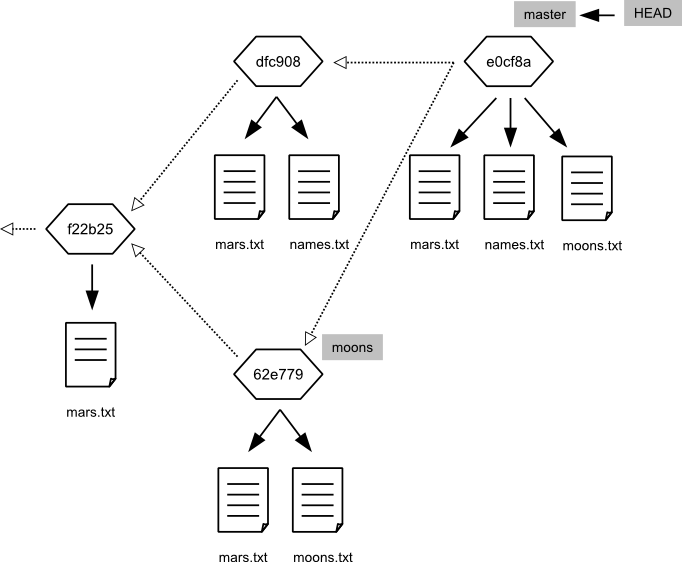
\includegraphics{novice/extras/img/git-branching-06.png}

We can ask Git to draw a diagram of the repository's history with this
command:

\begin{verbatim}
$ git log --oneline --topo-order --graph
\end{verbatim}

\begin{verbatim}
*   e0cf8ab Merge branch 'moons'
|\
| * 62e7791 Thinking about the moons
* | dfcf908 We will need a cool name for our secret base
|/
* 005937f Thoughts about the climate
* 34961b1 Concerns about Mars's moons on my furry friend
* f22b25e Starting to think about Mars
\end{verbatim}

This ASCII art is fine for small sets of changes, but for anything
significant, it's much better to use a GUI that can draw graphs using
lines instead of characters.

Branching strikes most newcomers as unnecessary complexity, particularly
for single-author projects. After all, if we need to make some changes
to a project, what do we gain by creating parallel universes?

The answer is that branching makes it easy for us to concentrate on one
thing at a time. Suppose we are part-way through rewriting a function
that calculates spatial correlations when we realize that the task would
be easier if our file I/O routines always stored things as complex
numbers. Most people would put the spatial correlation changes aside,
change the file I/O, then (hopefully) come back to the original task.

The problem with this is that we have to remember what we were doing,
even if we realize halfway through rewriting file I/O that we should
also rewrite our error handling. It's quite common to wind up with half
a dozen tasks stacked on top of one another, and quite hard to them all
straight. Branching allows us to put what we're doing in a safe place,
solve the new problem, then resume our earlier work.

In practice, most developers never make changes directly in the
\texttt{master} branch. Instead, they create a new branch from it for
every change they want to make, then merge those branches back to
\texttt{master} when the work is complete. Returning to our hypothetical
example, we would:

\begin{swcenumerate}
\item
  create a branch called something like
  \texttt{better-spatial-correlation} for those changes;
\item
  go back to master and create another branch called
  \texttt{file-input-produces-complex-values} for \emph{those} changes;
\item
  merge \texttt{file-input-produces-complex-values} into
  \texttt{master};
\item
  merge \texttt{master} into \texttt{better-spatial-correlation}; and
\item
  finish work on the spatial correlation function and merge it all back
  into \texttt{master}.
\end{swcenumerate}

And if, partway through this process, our supervisor asked us to change
the graph-plotting routines to conform to the university's new style
guide, we would simply switch back to \texttt{master}, create a branch
for that, make the changes, produce the desired graphs, and leave the
changes parked in that branch until we were ready to merge them.

\section{Code Review}

The model shown in the \urlfoot{../git/02-collab.html}{main lesson} in
which everyone pushes and pulls from a single repository, is perfectly
usable, but there's one thing it \emph{doesn't} let us do:
\gl{code review}{g:code-review}. Suppose Dracula wants to be able
to look at Wolfman's changes before merging them into the master copy on
GitHub, just as he would review Wolfman's paper before publishing it (or
perhaps even before submitting it for publication). We need to arrange
things so that Wolfman can commit his changes and Dracula can compare
them with the master copy; in fact, we want Wolfman to be able to commit
many times, so that he can incorporate Dracula's feedback and get
further review as often as necessary.

To allow code review, most programmers take a slightly more roundabout
route to merging. When the project starts, Dracula creates a repository
on GitHub in exactly the same way as \urlfoot{../git/02-collab.html}{we
created the \texttt{planets} repository} and then
\gl{clones}{g:repository-clone} it to his desktop:

\begin{verbatim}
$ git clone https://github.com/vlad/undersea.git
\end{verbatim}

\begin{verbatim}
Cloning into 'undersea'...
warning: You appear to have cloned an empty repository.
\end{verbatim}

\texttt{git clone} automatically adds the original repository on GitHub
as a remote of the local repository called \texttt{origin}---this is why
we chose \texttt{origin} as a remote name in our previous example:

\begin{verbatim}
$ cd undersea
$ git remote -v
\end{verbatim}

\begin{verbatim}
origin https://github.com/vlad/undersea.git (fetch)
origin https://github.com/vlad/undersea.git (push)
\end{verbatim}

Dracula can now push and pull changes just as before.

Wolfman doesn't clone Dracula's GitHub repository directly. Instead, he
\gl{forks}{g:repository-fork} it, i.e., clones it on GitHub. He
does this using the GitHub web interface:


\includegraphics{novice/extras/img/git-fork-ui.png}

He then clones his own GitHub repository, not Dracula's, to give himself
a desktop copy:

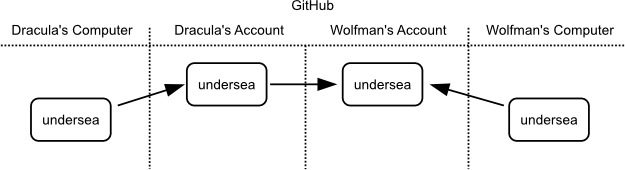
\includegraphics{novice/extras/img/git-forking-01.png}

This may seem like unnecessary work, but it allows Wolfman and Dracula
to collaborate much more effectively. Suppose Wolfman makes a change to
the project. He commits it to his local repository, then uses
\texttt{git push} to copy those changes to GitHub:

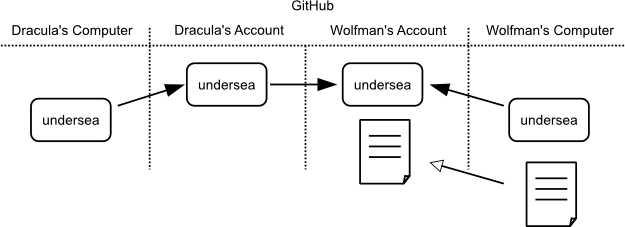
\includegraphics{novice/extras/img/git-forking-02.png}

He then creates a \gl{pull request}{g:pull-request}, which
notifies Dracula that Wolfman wants to merge some changes into Dracula's
repository:

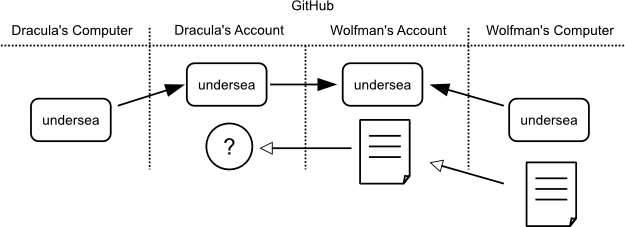
\includegraphics{novice/extras/img/git-forking-03.png}

A pull request is a merge waiting to happen. When Dracula views it
online, he can see and comment on the changes Wolfman wants to make.
Commenting is the crucial step here, and half the reason Wolfman went to
the trouble of forking the repository on GitHub. Dracula, or anyone else
involved in the project, can now give Wolfman feedback on what he is
trying to do: this function is too long, that one contains a bug,
there's a special case that isn't being handled anywhere, and so on.
Wolfman can then update his code, commit locally, and push those changes
to GitHub to update the pull request.

This process is exactly like peer review of papers, though usually much
faster. In large open source projects like Firefox, it's very common for
a pull request to be updated several times before finally being accepted
and merged. Working this way not only helps maintain the quality of the
code, it is also a very effective way to transfer knowledge.

If Wolfman wants to do more work while he's waiting for Dracula to
review his first modification, he creates a new branch in his local
repository, pushes it to GitHub, and then issues a pull request from
that. We can now see why Git, Mercurial, and other modern version
control systems use branching so much: it helps people work together,
but on their own time. It might take Dracula several days to get around
to reviewing Wolfman's changes. Rather than being stalled until then,
Wolfman can just switch to another branch and work on something else,
then switch back when Dracula's review finally comes in. Once the
changes in a particular branch have been accepted, Wolfman can delete
it; provided it has been merged into \texttt{master} (or some other
branch), the only thing that will be lost is the pointer with the branch
name, not the changes themselves.

We said above that code review is half the reason every developer should
have their own repository on GitHub (or whatever service is being used).
The other reason is that working this way allows people to explore ideas
without needing permission from any central authority. If you want to
change this tutorial, you can fork the
\urlfoot{https://github.com/swcarpentry/bc}{Software Carpentry repository
on GitHub} and start rewriting things in your repository. You can send
us a pull request if you want to share you changes with us, but you
don't have to. And if other people like your version better than ours,
they can start forking your repository and sending pull requests to you
instead of to us.

If this sounds familiar, it's because it is the way science itself
works. When someone publishes a new method or result, other scientists
can immediately start building on top of it---essentially, they can
create their own fork of the work and start committing changes to it. If
the first scientist likes the second's work, she can incorporate those
findings into her next paper, which is analogous to merging a pull
request. If she doesn't, then it's up to other scientists to decide
whose work to build on, or whether to try to combine both approaches.

\section{Manual Pages}

We can get help for any Unix command with the \texttt{man} (short for
manual) command. For example, here is the command to look up information
on \texttt{cp}:

\begin{verbatim}
$ man cp
\end{verbatim}

The output displayed is referred to as the ``man page''.

The man page will be displayed in the default file viewer for our shell,
which usually a program called \texttt{more}. When \texttt{more}
displays a colon `:', we can press the space bar to get the next page,
the letter `h' to get help, or the letter `q' to quit.

\texttt{man}'s output is typically complete but concise, as it is
designed to be used as a reference rather than a tutorial. Most man
pages are divided into sections:

\begin{swcitemize}
\item
  NAME: gives the name of the command and a brief description
\item
  SYNOPSIS: how to run the command, including optional and mandatory
  parameters. (We will explain the syntax later.)
\item
  DESCRIPTION: a fuller description than the synopsis, including a
  description of all the options to the command. This section may also
  include example usage or details about how the command works.
\item
  EXAMPLES: self-explanatory.
\item
  SEE ALSO: list other commands that we might find useful or other
  sources of information that might help us.
\end{swcitemize}

Other sections we might see include AUTHOR, REPORTING BUGS, COPYRIGHT,
HISTORY, (known) BUGS, and COMPATIBILITY.

\mbox{}\paragraph{How to Read the Synopsis}

Here is the is synopsis for the \texttt{cp} command on Ubuntu Linux:

\begin{verbatim}
SYNOPSIS
   cp [OPTION]... [-T] SOURCE DEST
   cp [OPTION]... SOURCE... DIRECTORY
   cp [OPTION]... -t DIRECTORY SOURCE...
\end{verbatim}

This tells the reader that there are three ways to use the command.
Let's look at the first usage:

\begin{verbatim}
cp [OPTION]... [-T] SOURCE DEST
\end{verbatim}

\texttt{{[}OPTION{]}} means the \texttt{cp} command can be followed by
one or more optional \gl{flags}{g:command-line-flag}. We can tell
they're optional because of the square brackets, and we can tell that
one or more are welcome because of the ellipsis (\ldots{}). For example,
the fact that \texttt{{[}-T{]}} is in square brackets, but after the
ellipsis, means that it's optional, but if it's used, it must come after
all the other options.

\texttt{SOURCE} refers to the source file or directory, and
\texttt{DEST} to the destination file or directory. Their precise
meanings are explained at the top of the \texttt{DESCRIPTION} section.

The other two usage examples can be read in similar ways. Note that to
use the last one, the \texttt{-t} option is mandatory (because it isn't
shown in square brackets).

The \texttt{DESCRIPTION} section starts with a few paragraphs explaining
the command and its use, then expands on the possible options one by
one:

\begin{verbatim}
     The following options are available:

     -a    Same as -pPR options. Preserves structure and attributes of
           files but not directory structure.

     -f    If the destination file cannot be opened, remove it and create
           a new file, without prompting for confirmation regardless of
           its permissions.  (The -f option overrides any previous -n
           option.)

           The target file is not unlinked before the copy.  Thus, any
           existing access rights will be retained.

      ...  ...
\end{verbatim}

\mbox{}\paragraph{Finding Help on Specific Options}

If we want to skip ahead to the option you're interested in, we can
search for it using the slash key `/'. (This isn't part of the
\texttt{man} command: it's a feature of \texttt{more}.) For example, to
find out about \texttt{-t}, we can type \texttt{/-t} and press return.
After that, we can use the `n' key to navigate to the next match until
we find the detailed information we need:

\begin{verbatim}
-t, --target-directory=DIRECTORY
     copy all SOURCE arguments into DIRECTORY
\end{verbatim}

This means that this option has the short form \texttt{-t} and the long
form \texttt{-{}-target-directory} and that it takes an argument. Its
meaning is to copy all the SOURCE arguments into DIRECTORY. Thus, we can
give the destination explicitly instead of relying on having to place
the directory at the end.

\mbox{}\paragraph{Limitations of Man Pages}

Man pages can be useful for a quick confirmation of how to run a
command, but they are not famous for being readable. If you can't find
what you need in the man page---or you can't understand what you've
found---try entering ``unix command copy file'' into your favorite
search engine: it will often produce more helpful results.

\begin{swcbox}{You May Also Enjoy\ldots{}}

The \urlfoot{http://explainshell.com/}{explainshell.com} site does a great
job of breaking complex Unix commands into parts and explaining what
each does. Sadly, it doesn't work in reverse\ldots{}

\end{swcbox}

\section{Permissions}

Unix controls who can read, modify, and run files using
\emph{permissions}. We'll discuss how Windows handles permissions at the
end of the section: the concepts are similar, but the rules are
different.

Let's start with Nelle. She has a unique \gl{user
name}{g:user-name}, \texttt{nnemo}, and a \gl{user ID}{g:user-id}, 1404.

\begin{swcbox}{Why Integer IDs?}

Why integers for IDs? Again, the answer goes back to the early 1970s.
Character strings like \texttt{alan.turing} are of varying length, and
comparing one to another takes many instructions. Integers, on the other
hand, use a fairly small amount of storage (typically four characters),
and can be compared with a single instruction. To make operations fast
and simple, programmers often keep track of things internally using
integers, then use a lookup table of some kind to translate those
integers into user-friendly text for presentation. Of course,
programmers being programmers, they will often skip the user-friendly
string part and just use the integers, in the same way that someone
working in a lab might talk about Experiment 28 instead of ``the
chronotypical alpha-response trials on anacondas''.

\end{swcbox}

Users can belong to any number of \gl{groups}{g:user-group}, each
of which has a unique \gl{group name}{g:user-group-name} and
numeric \gl{group ID}{g:user-group-id}. The list of who's in what
group is usually stored in the file \texttt{/etc/group}. (If you're in
front of a Unix machine right now, try running \texttt{cat /etc/group}
to look at that file.)

Now let's look at files and directories. Every file and directory on a
Unix computer belongs to one owner and one group. Along with each file's
content, the operating system stores the numeric IDs of the user and
group that own it.

The user-and-group model means that for each file every user on the
system falls into one of three categories: the owner of the file,
someone in the file's group, and everyone else.

For each of these three categories, the computer keeps track of whether
people in that category can read the file, write to the file, or execute
the file (i.e., run it if it is a program).

For example, if a file had the following set of permissions:

user

group

all

read

yes

yes

no

write

yes

no

no

execute

no

no

no

it would mean that:

\begin{swcitemize}
\item
  the file's owner can read and write it, but not run it;
\item
  other people in the file's group can read it, but not modify it or run
  it; and
\item
  everybody else can do nothing with it at all.
\end{swcitemize}

Let's look at this model in action. If we \texttt{cd} into the
\texttt{labs} directory and run \texttt{ls -F}, it puts a \texttt{*} at
the end of \texttt{setup}'s name. This is its way of telling us that
\texttt{setup} is executable, i.e., that it's (probably) something the
computer can run.

\begin{verbatim}
$ cd labs
$ ls -F
\end{verbatim}

\begin{verbatim}
safety.txt    setup*     waiver.txt
\end{verbatim}

\begin{swcbox}{Necessary But Not Sufficient}

The fact that something is marked as executable doesn't actually mean it
contains a program of some kind. We could easily mark this HTML file as
executable using the commands that are introduced below. Depending on
the operating system we're using, trying to ``run'' it will either fail
(because it doesn't contain instructions the computer recognizes) or
cause the operating system to open the file with whatever application
usually handles it (such as a web browser).

\end{swcbox}

Now let's run the command \texttt{ls -l}:

\begin{verbatim}
$ ls -l
\end{verbatim}

\begin{verbatim}
-rw-rw-r-- 1 vlad bio  1158  2010-07-11 08:22 safety.txt
-rwxr-xr-x 1 vlad bio 31988  2010-07-23 20:04 setup
-rw-rw-r-- 1 vlad bio  2312  2010-07-11 08:23 waiver.txt
\end{verbatim}

The \texttt{-l} flag tells \texttt{ls} to give us a long-form listing.
It's a lot of information, so let's go through the columns in turn.

On the right side, we have the files' names. Next to them, moving left,
are the times and dates they were last modified. Backup systems and
other tools use this information in a variety of ways, but you can use
it to tell when you (or anyone else with permission) last changed a
file.

Next to the modification time is the file's size in bytes and the names
of the user and group that owns it (in this case, \texttt{vlad} and
\texttt{bio} respectively). We'll skip over the second column for now
(the one showing \texttt{1} for each file) because it's the first column
that we care about most. This shows the file's permissions, i.e., who
can read, write, or execute it.

Let's have a closer look at one of those permission strings:
\texttt{-rwxr-xr-x}. The first character tells us what type of thing
this is: `-' means it's a regular file, while `d' means it's a
directory, and other characters mean more esoteric things.

The next three characters tell us what permissions the file's owner has.
Here, the owner can read, write, and execute the file: \texttt{rwx}. The
middle triplet shows us the group's permissions. If the permission is
turned off, we see a dash, so \texttt{r-x} means ``read and execute, but
not write''. The final triplet shows us what everyone who isn't the
file's owner, or in the file's group, can do. In this case, it's `r-x'
again, so everyone on the system can look at the file's contents and run
it.

To change permissions, we use the \texttt{chmod} command (whose name
stands for ``change mode''). Here's a long-form listing showing the
permissions on the final grades in the course Vlad is teaching:

\begin{verbatim}
$ ls -l final.grd
\end{verbatim}

\begin{verbatim}
-rwxrwxrwx 1 vlad bio  4215  2010-08-29 22:30 final.grd
\end{verbatim}

Whoops: everyone in the world can read it---and what's worse, modify it!
(They could also try to run the grades file as a program, which would
almost certainly not work.)

The command to change the owner's permissions to \texttt{rw-} is:

\begin{verbatim}
$ chmod u=rw final.grd
\end{verbatim}

The `u' signals that we're changing the privileges of the user (i.e.,
the file's owner), and \texttt{rw} is the new set of permissions. A
quick \texttt{ls -l} shows us that it worked, because the owner's
permissions are now set to read and write:

\begin{verbatim}
$ ls -l final.grd
\end{verbatim}

\begin{verbatim}
-rw-rwxrwx 1 vlad bio  4215  2010-08-30 08:19 final.grd
\end{verbatim}

Let's run \texttt{chmod} again to give the group read-only permission:

\begin{verbatim}
$ chmod g=r final.grd
$ ls -l final.grd
\end{verbatim}

\begin{verbatim}
-rw-r--rw- 1 vlad bio  4215  2010-08-30 08:19 final.grd
\end{verbatim}

And finally, let's give ``all'' (everyone on the system who isn't the
file's owner or in its group) no permissions at all:

\begin{verbatim}
$ chmod a= final.grd
$ ls -l final.grd
\end{verbatim}

\begin{verbatim}
-rw-r----- 1 vlad bio  4215  2010-08-30 08:20 final.grd
\end{verbatim}

Here, the `a' signals that we're changing permissions for ``all'', and
since there's nothing on the right of the ``='', ``all'''s new
permissions are empty.

We can search by permissions, too. Here, for example, we can use
\texttt{-type f -perm -u=x} to find files that the user can execute:

\begin{verbatim}
$ find . -type f -perm -u=x
\end{verbatim}

\begin{verbatim}
./tools/format
./tools/stats
\end{verbatim}

Before we go any further, let's run \texttt{ls -a -l} to get a long-form
listing that includes directory entries that are normally hidden:

\begin{verbatim}
$ ls -a -l
\end{verbatim}

\begin{verbatim}
drwxr-xr-x 1 vlad bio     0  2010-08-14 09:55 .
drwxr-xr-x 1 vlad bio  8192  2010-08-27 23:11 ..
-rw-rw-r-- 1 vlad bio  1158  2010-07-11 08:22 safety.txt
-rwxr-xr-x 1 vlad bio 31988  2010-07-23 20:04 setup
-rw-rw-r-- 1 vlad bio  2312  2010-07-11 08:23 waiver.txt
\end{verbatim}

The permissions for \texttt{.} and \texttt{..} (this directory and its
parent) start with a `d'. But look at the rest of their permissions: the
`x' means that ``execute'' is turned on. What does that mean? A
directory isn't a program---how can we ``run'' it?

In fact, `x' means something different for directories. It gives someone
the right to \emph{traverse} the directory, but not to look at its
contents. The distinction is subtle, so let's have a look at an example.
Vlad's home directory has three subdirectories called \texttt{venus},
\texttt{mars}, and \texttt{pluto}:

\includegraphics{novice/extras/img/x-for-directories.png}

Each of these has a subdirectory in turn called \texttt{notes}, and
those sub-subdirectories contain various files. If a user's permissions
on \texttt{venus} are `r-x', then if she tries to see the contents of
\texttt{venus} and \texttt{venus/notes} using \texttt{ls}, the computer
lets her see both. If her permissions on \texttt{mars} are just `r--',
then she is allowed to read the contents of both \texttt{mars} and
\texttt{mars/notes}. But if her permissions on \texttt{pluto} are only
`--x', she cannot see what's in the \texttt{pluto} directory:
\texttt{ls pluto} will tell her she doesn't have permission to view its
contents. If she tries to look in \texttt{pluto/notes}, though, the
computer will let her do that. She's allowed to go through
\texttt{pluto}, but not to look at what's there. This trick gives people
a way to make some of their directories visible to the world as a whole
without opening up everything else.

\mbox{}\paragraph{What about Windows?}

Those are the basics of permissions on Unix. As we said at the outset,
though, things work differently on Windows. There, permissions are
defined by \gl{access control lists}{g:access-control-list}, or
ACLs. An ACL is a list of pairs, each of which combines a ``who'' with a
``what''. For example, you could give the Mummy permission to append
data to a file without giving him permission to read or delete it, and
give Frankenstein permission to delete a file without being able to see
what it contains.

This is more flexible that the Unix model, but it's also more complex to
administer and understand on small systems. (If you have a large
computer system, \emph{nothing} is easy to administer or understand.)
Some modern variants of Unix support ACLs as well as the older
read-write-execute permissions, but hardly anyone uses them.

\section{Shell Variables}

The shell is just a program, and like other programs, it has variables.
Those variables control its execution, so by changing their values you
can change how the shell and other programs behave.

Let's start by running the command \texttt{set} and looking at some of
the variables in a typical shell session:

\begin{verbatim}
$ set
\end{verbatim}

\begin{verbatim}
COMPUTERNAME=TURING
HOME=/home/vlad
HOMEDRIVE=C:
HOSTNAME=TURING
HOSTTYPE=i686
NUMBER_OF_PROCESSORS=4
OS=Windows_NT
PATH=/Users/vlad/bin:/usr/local/git/bin:/usr/bin:/bin:/usr/sbin:/sbin:/usr/local/bin
PWD=/home/vlad
UID=1000
USERNAME=vlad
...
\end{verbatim}

As you can see, there are quite a few---in fact, four or five times more
than what's shown here. And yes, using \texttt{set} to \emph{show}
things might seem a little strange, even for Unix, but if you don't give
it any arguments, it might as well show you things you \emph{could} set.

Every variable has a name. By convention, variables that are always
present are given upper-case names. All shell variables' values are
strings, even those (like \texttt{UID}) that look like numbers. It's up
to programs to convert these strings to other types when necessary. For
example, if a program wanted to find out how many processors the
computer had, it would convert the value of the
\texttt{NUMBER\_OF\_PROCESSORS} variable from a string to an integer.

Similarly, some variables (like \texttt{PATH}) store lists of values. In
this case, the convention is to use a colon `:' as a separator. If a
program wants the individual elements of such a list, it's the program's
responsibility to split the variable's string value into pieces.

\mbox{}\paragraph{The \texttt{PATH} Variable}

Let's have a closer look at that \texttt{PATH} variable. Its value
defines the shell's \gl{search path}{g:search-path}, i.e., the
list of directories that the shell looks in for runnable programs when
you type in a program name without specifying what directory it is in.

For example, when we type a command like \texttt{analyze}, the shell
needs to decide whether to run \texttt{./analyze} or
\texttt{/bin/analyze}. The rule it uses is simple: the shell checks each
directory in the \texttt{PATH} variable in turn, looking for a program
with the requested name in that directory. As soon as it finds a match,
it stops searching and runs the program.

To show how this works, here are the components of \texttt{PATH} listed
one per line:

\begin{verbatim}
/Users/vlad/bin
/usr/local/git/bin
/usr/bin
/bin
/usr/sbin
/sbin
/usr/local/bin
\end{verbatim}

On our computer, there are actually three programs called
\texttt{analyze} in three different directories: \texttt{/bin/analyze},
\texttt{/usr/local/bin/analyze}, and \texttt{/users/vlad/analyze}. Since
the shell searches the directories in the order they're listed in
\texttt{PATH}, it finds \texttt{/bin/analyze} first and runs that.
Notice that it will \emph{never} find the program
\texttt{/users/vlad/analyze} unless we type in the full path to the
program, since the directory \texttt{/users/vlad} isn't in
\texttt{PATH}.

\mbox{}\paragraph{Showing the Value of a Variable}

Let's show the value of the variable \texttt{HOME}:

\begin{verbatim}
$ echo HOME
\end{verbatim}

\begin{verbatim}
HOME
\end{verbatim}

That just prints ``HOME'', which isn't what we wanted (though it is what
we actually asked for). Let's try this instead:

\begin{verbatim}
$ echo $HOME
\end{verbatim}

\begin{verbatim}
/home/vlad
\end{verbatim}

The dollar sign tells the shell that we want the \emph{value} of the
variable rather than its name. This works just like wildcards: the shell
does the replacement \emph{before} running the program we've asked for.
Thanks to this expansion, what we actually run is
\texttt{echo /home/vlad}, which displays the right thing.

\mbox{}\paragraph{Creating and Changing Variables}

Creating a variable is easy---we just assign a value to a name using
``='':

\begin{verbatim}
$ SECRET_IDENTITY=Dracula
$ echo $SECRET_IDENTITY
\end{verbatim}

\begin{verbatim}
Dracula
\end{verbatim}

To change the value, just assign a new one:

\begin{verbatim}
$ SECRET_IDENTITY=Camilla
$ echo $SECRET_IDENTITY
\end{verbatim}

\begin{verbatim}
Camilla
\end{verbatim}

If we want to set some variables automatically every time we run a
shell, we can put commands to do this in a file called \texttt{.bashrc}
in our home directory. (The `.' character at the front prevents
\texttt{ls} from listing this file unless we specifically ask it to
using \texttt{-a}: we normally don't want to worry about it. The ``rc''
at the end is an abbreviation for ``run control'', which meant something
really important decades ago, and is now just a convention everyone
follows without understanding why.)

For example, here are two lines in \texttt{/home/vlad/.bashrc}:

\begin{verbatim}
export SECRET_IDENTITY=Dracula
export TEMP_DIR=/tmp
export BACKUP_DIR=$TEMP_DIR/backup
\end{verbatim}

These three lines create the variables \texttt{SECRET\_IDENTITY},
\texttt{TEMP\_DIR}, and \texttt{BACKUP\_DIR}, and export them so that
any programs the shell runs can see them as well. Notice that
\texttt{BACKUP\_DIR}'s definition relies on the value of
\texttt{TEMP\_DIR}, so that if we change where we put temporary files,
our backups will be relocated automatically.

While we're here, it's also common to use the \texttt{alias} command to
create shortcuts for things we frequently type. For example, we can
define the alias \texttt{backup} to run \texttt{/bin/zback} with a
specific set of arguments:

\begin{verbatim}
alias backup=/bin/zback -v --nostir -R 20000 $HOME $BACKUP_DIR
\end{verbatim}

As you can see, aliases can save us a lot of typing, and hence a lot of
typing mistakes. You can find interesting suggestions for other aliases
and other bash tricks by searching for ``sample bashrc'' in your
favorite search engine.

\section{Working Remotely}

Let's take a closer look at what happens when we use the shell on a
desktop or laptop computer. The first step is to log in so that the
operating system knows who we are and what we're allowed to do. We do
this by typing our username and password; the operating system checks
those values against its records, and if they match, runs a shell for
us.

As we type commands, the 1's and 0's that represent the characters we're
typing are sent from the keyboard to the shell. The shell displays those
characters on the screen to represent what we type, and then, if what we
typed was a command, the shell executes it and displays its output (if
any).

What if we want to run some commands on another machine, such as the
server in the basement that manages our database of experimental
results? To do this, we have to first log in to that machine. We call
this a \gl{remote login}{g:remote-login}, and the other computer a
remote computer. Once we do this, everything we type is passed to a
shell running on the remote computer. That shell runs those commands on
our behalf, just as a local shell would, then sends back output for our
computer to display.

The tool we use to log in remotely is the {[}secure
shell)(\#g:secure-shell), or SSH. In particular, the command
\texttt{ssh username@computer} runs SSH and connects to the remote
computer we have specified. After we log in, we can use the remote shell
to use the remote computer's files and directories. Typing \texttt{exit}
or Control-D terminates the remote shell and returns us to our previous
shell.

In the example below, the remote machine's command prompt is
\texttt{moon\textgreater{}} instead of just \texttt{\$}. To make it
clearer which machine is doing what, we'll indent the commands sent to
the remote machine and their output.

\begin{verbatim}
$ pwd
\end{verbatim}

\begin{verbatim}
/users/vlad
\end{verbatim}

\begin{verbatim}
$ ssh vlad@moon.euphoric.edu
Password: ********
\end{verbatim}

\begin{verbatim}
    moon> hostname
\end{verbatim}

\begin{verbatim}
    moon
\end{verbatim}

\begin{verbatim}
    moon> pwd
\end{verbatim}

\begin{verbatim}
    /home/vlad
\end{verbatim}

\begin{verbatim}
    moon> ls -F
\end{verbatim}

\begin{verbatim}
    bin/     cheese.txt   dark_side/   rocks.cfg
\end{verbatim}

\begin{verbatim}
    moon> exit
\end{verbatim}

\begin{verbatim}
$ pwd
\end{verbatim}

\begin{verbatim}
/users/vlad
\end{verbatim}

The secure shell is called ``secure'' to contrast it with an older
program called \texttt{rsh}, which stood for ``remote shell''. Back in
the day, when everyone trusted each other and knew every chip in their
computer by its first name, people didn't encrypt anything except the
most sensitive information when sending it over a network. However, that
meant that villains could watch network traffic, steal usernames and
passwords, and use them for all manner of nefarious purposes. SSH was
invented to prevent this (or at least slow it down). It uses several
sophisticated, and heavily tested, encryption protocols to ensure that
outsiders can't see what's in the messages going back and forth between
different computers.

\texttt{ssh} has a companion program called \texttt{scp}, which stands
for ``secure copy''. It allows us to copy files to or from a remote
computer using the same kind of connection as SSH. The command's name
combines \texttt{cp}'s and \texttt{ssh}'s, and so does its operation. To
copy a file, we specify the source and destination paths, either of
which may include computer names. If we leave out a computer name,
\texttt{scp} assumes we mean the machine we're running on. For example,
this command copies our latest results to the backup server in the
basement, printing out its progress as it does so:

\begin{verbatim}
$ scp results.dat vlad@backupserver:backups/results-2011-11-11.dat
Password: ********
\end{verbatim}

\begin{verbatim}
results.dat              100%  9  1.0 MB/s 00:00
\end{verbatim}

Copying a whole directory is similar: we just use the \texttt{-r} option
to signal that we want copying to be recursive. For example, this
command copies all of our results from the backup server to our laptop:

\begin{verbatim}
$ scp -r vlad@backupserver:backups ./backups
Password: ********
\end{verbatim}

\begin{verbatim}
results-2011-09-18.dat              100%  7  1.0 MB/s 00:00
results-2011-10-04.dat              100%  9  1.0 MB/s 00:00
results-2011-10-28.dat              100%  8  1.0 MB/s 00:00
results-2011-11-11.dat              100%  9  1.0 MB/s 00:00
\end{verbatim}

Here's one more thing SSH can do for us. Suppose we want to check
whether we have already created the file
\texttt{backups/results-2011-11-12.dat} on the backup server. Instead of
logging in and then typing \texttt{ls}, we could do this:

\begin{verbatim}
$ ssh vlad@backupserver "ls results"
Password: ********
\end{verbatim}

\begin{verbatim}
results-2011-09-18.dat  results-2011-10-28.dat
results-2011-10-04.dat  results-2011-11-11.dat
\end{verbatim}

SSH takes the argument after our remote username and passes them to the
shell on the remote computer. (We have to put quotes around it to make
it look like a single argument.) Since those arguments are a legal
command, the remote shell runs \texttt{ls results} for us and sends the
output back to our local shell for display.

\begin{swcbox}{All Those Passwords}

Typing our password over and over again is annoying, especially if the
commands we want to run remotely are in a loop. To remove the need to do
this, we can create an \gl{authentication
key}{g:authentication-key} to tell the remote machine that it should always trust us. We
discuss authentication keys in our intermediate lessons.

\end{swcbox}

\section{Exceptions}

Assertions help us catch errors in our code, but things can go wrong for
other reasons, like missing or badly-formatted files. Most modern
programming languages allow programmers to use
\gl{exceptions}{g:exception} to separate what the program should
do if everything goes right from what it should do if something goes
wrong. Doing this makes both cases easier to read and understand.

For example, here's a small piece of code that tries to read parameters
and a grid from two separate files, and reports an error if either goes
wrong:

\begin{verbatim}
try:
    params = read_params(param_file)
    grid = read_grid(grid_file)
except:
    log.error('Failed to read input file(s)')
    sys.exit(ERROR)
\end{verbatim}

We join the normal case and the error-handling code using the keywords
\texttt{try} and \texttt{except}. These work together like \texttt{if}
and \texttt{else}: the statements under the \texttt{try} are what should
happen if everything works, while the statements under \texttt{except}
are what the program should do if something goes wrong.

We have actually seen exceptions before without knowing it, since by
default, when an exception occurs, Python prints it out and halts our
program. For example, trying to open a nonexistent file triggers a type
of exception called an \texttt{IOError}, while trying to access a list
element that doesn't exist causes an \texttt{IndexError}:

\begin{verbatim}
open('nonexistent-file.txt', 'r')
\end{verbatim}

\begin{verbatim}
---------------------------------------------------------------------------
IOError                                   Traceback (most recent call last)

<ipython-input-13-58cbde3dd63c> in <module>()
----> 1 open('nonexistent-file.txt', 'r')

IOError: [Errno 2] No such file or directory: 'nonexistent-file.txt'
\end{verbatim}

\begin{verbatim}
values = [0, 1, 2]
print values[999]
\end{verbatim}

\begin{verbatim}
---------------------------------------------------------------------------
IndexError                                Traceback (most recent call last)

<ipython-input-14-7fed13afc650> in <module>()
1 values = [0, 1, 2]
----> 2 print values[999]

IndexError: list index out of range
\end{verbatim}

We can use \texttt{try} and \texttt{except} to deal with these errors
ourselves if we don't want the program simply to fall over:

\begin{verbatim}
try:
    reader = open('nonexistent-file.txt', 'r')
except IOError:
    print 'Whoops!'
\end{verbatim}

\begin{verbatim}
Whoops!
\end{verbatim}

When Python executes this code, it runs the statement inside the
\texttt{try}. If that works, it skips over the \texttt{except} block
without running it. If an exception occurs inside the \texttt{try}
block, though, Python compares the type of the exception to the type
specified by the \texttt{except}. If they match, it executes the code in
the \texttt{except} block.

\texttt{IOError} is the particular kind of exception Python raises when
there is a problem related to input and output, such as files not
existing or the program not having the permissions it needs to read
them. We can put as many lines of code in a \texttt{try} block as we
want, just as we can put many statements under an \texttt{if}. We can
also handle several different kinds of errors afterward. For example,
here's some code to calculate the entropy at each point in a grid:

\begin{verbatim}
try:
    params = read_params(param_file)
    grid = read_grid(grid_file)
    entropy = lee_entropy(params, grid)
    write_entropy(entropy_file, entropy)
except IOError:
    report_error_and_exit('IO error')
except ArithmeticError:
    report_error_and_exit('Arithmetic error')
\end{verbatim}

Python tries to run the four functions inside the \texttt{try} as
normal. If an error occurs in any of them, Python immediately jumps down
and tries to find an \texttt{except} of the corresponding type: if the
exception is an \texttt{IOError}, Python jumps into the first error
handler, while if it's an \texttt{ArithmeticError}, Python jumps into
the second handler instead. It will only execute one of these, just as
it will only execute one branch of a series of
\texttt{if}/\texttt{elif}/\texttt{else} statements.

This layout has made the code easier to read, but we've lost something
important: the message printed out by the \texttt{IOError} branch
doesn't tell us which file caused the problem. We can do better if we
capture and hang on to the object that Python creates to record
information about the error:

\begin{verbatim}
try:
    params = read_params(param_file)
    grid = read_grid(grid_file)
    entropy = lee_entropy(params, grid)
    write_entropy(entropy_file, entropy)
except IOError as err:
    report_error_and_exit('Cannot read/write' + err.filename)
except ArithmeticError as err:
    report_error_and_exit(err.message)
\end{verbatim}

If something goes wrong in the \texttt{try}, Python creates an exception
object, fills it with information, and assigns it to the variable
\texttt{err}. (There's nothing special about this variable name---we can
use anything we want.) Exactly what information is recorded depends on
what kind of error occurred; Python's documentation describes the
properties of each type of error in detail, but we can always just print
the exception object. In the case of an I/O error, we print out the name
of the file that caused the problem. And in the case of an arithmetic
error, printing out the message embedded in the exception object is what
Python would have done anyway.

So much for how exceptions work: how should they be used? Some
programmers use \texttt{try} and \texttt{except} to give their programs
default behaviors. For example, if this code can't read the grid file
that the user has asked for, it creates a default grid instead:

\begin{verbatim}
try:
    grid = read_grid(grid_file)
except IOError:
    grid = default_grid()
\end{verbatim}

Other programmers would explicitly test for the grid file, and use
\texttt{if} and \texttt{else} for control flow:

\begin{verbatim}
if file_exists(grid_file):
    grid = read_grid(grid_file)
else:
    grid = default_grid()
\end{verbatim}

It's mostly a matter of taste, but we prefer the second style. As a
rule, exceptions should only be used to handle exceptional cases. If the
program knows how to fall back to a default grid, that's not an
unexpected event. Using \texttt{if} and \texttt{else} instead of
\texttt{try} and \texttt{except} sends different signals to anyone
reading our code, even if they do the same thing.

Novices often ask another question about exception handling style, but
before we address it, there's something in our example that you might
not have noticed. Exceptions can actually be thrown a long way: they
don't have to be handled immediately. Take another look at this code:

\begin{verbatim}
try:
    params = read_params(param_file)
    grid = read_grid(grid_file)
    entropy = lee_entropy(params, grid)
    write_entropy(entropy_file, entropy)
except IOError as err:
    report_error_and_exit('Cannot read/write' + err.filename)
except ArithmeticError as err:
    report_error_and_exit(err.message)
\end{verbatim}

The four lines in the \texttt{try} block are all function calls. They
might catch and handle exceptions themselves, but if an exception occurs
in one of them that \emph{isn't} handled internally, Python looks in the
calling code for a matching \texttt{except}. If it doesn't find one
there, it looks in that function's caller, and so on. If we get all the
way back to the main program without finding an exception handler,
Python's default behavior is to print an error message like the ones
we've been seeing all along.

This rule is the origin of the rule
\urlfoot{../rules.html\#throw-low-catch-high}{throw low, catch high}. There
are many places in our program where an error might occur. There are
only a few, though, where errors can sensibly be handled. For example, a
linear algebra library doesn't know whether it's being called directly
from the Python interpreter, or whether it's being used as a component
in a larger program. In the latter case, the library doesn't know if the
program that's calling it is being run from the command line or from a
GUI. The library therefore shouldn't try to handle or report errors
itself, because it has no way of knowing what the right way to do this
is. It should instead just raise an exception, and let its caller figure
out how best to handle it.

Finally, we can raise exceptions ourselves if we want to. In fact, we
\emph{should} do this, since it's the standard way in Python to signal
that something has gone wrong. Here, for example, is a function that
reads a grid and checks its consistency:

\begin{verbatim}
def read_grid(grid_file):
    data = read_raw_data(grid_file)
    if not grid_consistent(data):
        raise Exception('Inconsistent grid: ' + grid_file)
    result = normalize_grid(data)
    return result
\end{verbatim}

The \texttt{raise} statement creates a new exception with a meaningful
error message. Since \texttt{read\_grid} itself doesn't contain a
\texttt{try}/\texttt{except} block, this exception will always be thrown
up and out of the function, to be caught and handled by whoever is
calling \texttt{read\_grid}. We can define new types of exceptions if we
want to. And we should, so that errors in our code can be distinguished
from errors in other people's code. However, this involves classes and
objects, which is outside the scope of these lessons.

\section{Numbers}

Let's start by looking at how numbers are stored. If we only have the
two digits 0 and 1, the natural way to store a positive integer is to
use base 2, so $1001_{2}$ is
$(1×2^{3})+(0×2^{2})+(0×2^{1})+(1×2^{0}) = 9_{10}$.
It's equally natural to extend this scheme to
negative numbers by reserving one bit for the sign. If, for example, we
use 0 for positive numbers and 1 for those that are negative,
$+9^{10}$ would be $01001^{2}$ and
$-9^{10}$ would be $11001^{10}$.

There are two problems with this. The first is that this scheme gives us
two representations for zero ($00000_{2}$ and
$10000_{2}$). This isn't necessarily fatal, but any claims
this scheme has to being ``natural'' disappear when we have to write
code like:

\begin{verbatim}
if (length != +0) and (length != -0)
\end{verbatim}

As for the other problem, it turns out that the circuits needed to do
addition and other arithmetic on this
\gl{sign and magnitude representation}{g:sign-and-magnitude} are
more complicated than the hardware needed for another called
\gl{two's complement}{g:twos-complement}. Instead of mirroring
positive values, two's complement rolls over when going below zero, just
like a car's odometer. If we're using four bits per number, so that
$0_{10}$ is $0000_{2}$, then $-1_{10}$
is $1111_{2}$. $-2_{10}$ is $1110_{2}$,
$-3_{10}$ is $1101_{2}$, and so on until we reach
the most negative number we can represent, $1000_{2}$, which
is -8. Our representation then wraps around again, so that
$0111_{2}$ is $7_{10}$.

This scheme isn't intuitive, but it solves sign and magnitude's ``double
zero'' problem, and the hardware to handle it is faster and cheaper. As
a bonus, we can still tell whether a number is positive or negative by
looking at the first bit: negative numbers have a 1, positives have a 0.
The only odd thing is its asymmetry: because 0 counts as a positive
number, numbers go from -8 to 7, or -16 to 15, and so on. As a result,
even if \texttt{x} is a valid number, \texttt{-x} may not be.

Finding a good representation for real numbers (called
\gl{floating point numbers}{g:floating-point}, since the decimal
point can move around) is a much harder problem. The root of the problem
is that we cannot represent an infinite number of real values with a
finite set of bit patterns. And unlike integers, no matter what values
we \emph{do} represent, there will be an infinite number of values
between each of them that we can't.

Floating point numbers are usually represented using sign, magnitude,
and an exponent. In a 32-bit word, the IEEE 754 standard calls for 1 bit
of sign, 23 bits for the magnitude (or \emph{mantissa}), and 8 bits for
the exponent. To illustrate the problems with floating point, we'll use
a much dumber representation: we'll only worry about positive values
without fractional parts, and we'll only use 3 for the magnitude and 2
for the exponent.

Exponent

00

01

10

11

000

0

0

0

0

001

1

2

4

8

010

2

4

8

16

Mantissa

011

3

6

12

24

100

4

8

16

32

101

5

10

20

40

110

6

12

24

48

111

7

14

28

56

The table above shows the values that we can represent this way. Each
one is the mantissa times two to the exponent. For example, the decimal
values 48 is binary 110 times 2 to the binary 11 power, which is 6 times
2 to the third, or 6 times 8. (Note that real floating point
representations like the IEEE 754 standard don't have the redundancy
shown in this table, but that doesn't affect our argument.)

The first thing you should notice is that there are a lot of values we
\emph{can't} store. We can do 8 and 10, for example, but not 9. This is
exactly like the problems hand calculators have with fractions like 1/3:
in decimal, we have to round that to 0.3333 or 0.3334.

But if this scheme has no representation for 9, then 8+1 must be stored
as either 8 or 10. This raises an interesting question: if 8+1 is 8,
what is 8+1+1? If we add from the left, 8+1 is 8, plus another 1 is 8
again. If we add from the right, though, 1+1 is 2, and 2+8 is 10.
Changing the order of operations can make the difference between right
and wrong. There's no randomness involved---a particular order of
operations will always produce the same result---but as the number of
steps increases, so too does the difficulty of figuring out what the
best order is.

This is the sort of problem that numerical analysts spend their time on.
In this case, if we sort the values we're adding, then add from smallest
to largest, it gives us a better chance of getting the best possible
answer. In other situations, like inverting a matrix, the rules are much
more complicated.

Here's another observation about our uneven number line: the spacing
between the values we can represent is uneven, but the relative spacing
between each set of values stays the same, i.e., the first group is
separated by 1, then the separation becomes 2, then 4, then 8, so that
the ratio of the spacing to the values stays roughly constant. This
happens because we're multiplying the same fixed set of mantissas by
ever-larger exponents, and it points us at a couple of useful
definitions.

The \gl{absolute error}{g:absolute-error} in some approximation is
simply the absolute value of the difference between the actual value and
the approximation. The \gl{relative error}{g:relative-error}, on
the other hand, is the ratio of the absolute error to the value we're
approximating. For example, if we're off by 1 in approximating 8+1 and
56+1, the absolute error is the same in both cases, but the relative
error in the first case is 1/9 = 11\%, while the relative error in the
second case is only 1/57 = 1.7\%. When we're thinking about floating
point numbers, relative error is almost always more useful than absolute
error. After all, it makes little sense to say that we're off by a
hundredth when the value in question is a billionth.

To see why this matters, let's have a look at a little program:

\begin{verbatim}
nines = []
sums = []
current = 0.0
for i in range(1, 10):
    num = 9.0 / (10.0 ** i)
    nines.append(num)
    current += num
    sums.append(current)

for i in range(len(nines)):
    print '%.18f %.18f' % (nines[i], sums[i])
\end{verbatim}

The loop runs over the integers from 1 to 9 inclusive. Using those
values, we create the numbers 0.9, 0.09, 0.009, and so on, and put them
in the list \texttt{vals}. We then calculate the sum of those numbers.
Clearly, this should be 0.9, 0.99, 0.999, and so on. But is it?

\begin{tabular}{lll}
\hline\noalign{\medskip}
1 & 0.900000000000000022 & 0.900000000000000022
\\\noalign{\medskip}
2 & 0.089999999999999997 & 0.989999999999999991
\\\noalign{\medskip}
3 & 0.008999999999999999 & 0.998999999999999999
\\\noalign{\medskip}
4 & 0.000900000000000000 & 0.999900000000000011
\\\noalign{\medskip}
5 & 0.000090000000000000 & 0.999990000000000046
\\\noalign{\medskip}
6 & 0.000009000000000000 & 0.999999000000000082
\\\noalign{\medskip}
7 & 0.000000900000000000 & 0.999999900000000053
\\\noalign{\medskip}
8 & 0.000000090000000000 & 0.999999990000000061
\\\noalign{\medskip}
9 & 0.000000009000000000 & 0.999999999000000028
\\\noalign{\medskip}
\hline
\end{tabular}

Here are our answers. The first column is the loop index; the second,
what we actually got when we tried to calculate 0.9, 0.09, and so on,
and the third is the cumulative sum.

The first thing you should notice is that the very first value
contributing to our sum is already slightly off. Even with 23 bits for a
mantissa, we cannot exactly represent 0.9 in base 2, any more than we
can exactly represent 1/3 in base 10. Doubling the size of the mantissa
would reduce the error, but we can't ever eliminate it.

The second thing to notice is that our approximation to 0.0009 actually
appears accurate, as do all of the approximations after that. This may
be misleading, though: after all, we've only printed things out to 18
decimal places. As for the errors in the last few digits of the sums,
there doesn't appear to be any regular pattern in the way they increase
and decrease.

This phenomenon is one of the things that makes testing scientific
programs hard. If a function uses floating point numbers, what do we
compare its result to if we want to check that it's working correctly?
If we compared the sum of the first few numbers in \texttt{vals} to what
it's supposed to be, the answer could be \texttt{False}, even if we're
initializing the list with the right values, and calculating the sum
correctly. This is a genuinely hard problem, and no one has a good
generic answer. The root of our problem is that we're using
approximations, and each approximation has to be judged on its own
merits.

There are things you can do, though. The first rule is, compare what you
get to analytic solutions whenever you can. For example, if you're
looking at the behavior of drops of liquid helium, start by checking
your program's output on a stationary spherical drop in zero gravity.
You should be able to calculate the right answer in that case, and if
your program doesn't work for that, it probably won't work for anything
else.

The second rule is to compare more complex versions of your code to
simpler ones. If you're about to replace a simple algorithm for
calculating heat transfer with one that's more complex, but hopefully
faster, don't throw the old code away. Instead, use its output as a
check on the correctness of the new code. And if you bump into someone
at a conference who has a program that can calculate some of the same
results as yours, swap data sets: it'll help you both.

The third rule is, never use \texttt{==} (or \texttt{!=}) on floating
point numbers, because two numbers calculated in different ways will
probably not have exactly the same bits. Instead, check to see whether
two values are within some tolerance, and if they are, treat them as
equal. Doing this forces you to make your tolerances explicit, which is
useful in its own right (just as putting error bars on experimental
results is useful).

\section{Why I Teach}

This is my daughter Madeline:

\includegraphics{novice/extras/img/madeleine.jpg}

Several independent studies have confirmed that she is the cutest child
on the planet (plus or minus 5\%, 19 times out of 20). She means the
world to me, but by the time she's grown, the world is going to be
dealing with the consequences of our generation's short-sightedness.
Climate change, resource shortages, drug-resistant diseases---the list
is a long one, and the only things that will save us are more science
and more courage.

That's why I teach. I teach because I need your help to make this world
fit for her to live in. I teach because I need you to discover more and
invent faster so that the world she inherits from you will be better
than the one you're inheriting from my generation. Science is not just
the greatest adventure of our time: it is, quite literally, a matter of
life and death, and I hope that what we have taught you will help you do
it better.

Thank you for your time: may you always see the world through the eyes
of a child.

\chapter{Instructor's Guide}\label{s:instructors}

As a species, we know a lot about how brains learn, how effective
various teaching practices are, and how society's needs and expectations
shape how and how well we learn. As individuals, though, most people who
teach at college and university either don't know this knowledge exists,
or haven't incorporated it into their teaching. It's as if only doctors
knew about the connection between smoking and cancer.

The best guide to evidence-based learning we have found is \emph{How
Learning Works: Seven Research-Based Principles for Smart Teaching} (see
the bibliography for the full citation). Its advice is based in equal
parts on theory, research, and experience. While some of the
recommendations may seem banal, the full-length explanations in the book
itself are anything but.

We try to incorporate these ideas into our teaching, and into our
\urlfoot{http://teaching.software-carpentry.org}{instructor training
course}. If you are interested in taking part, please get in touch.

\section{General Advice}

This is a placeholder for general notes about teaching. For up-to-date
information about software installation and configuration problems, and
their solutions, see
\urlfoot{https://github.com/swcarpentry/bc/wiki/Configuration-Problems-and-Solutions}{this
wiki page}.

\mbox{}\paragraph{Teaching Notes}

\begin{swcitemize}
\item
  For bootcamps that extend over more than two days (e.g., four
  afternoons spread over two weeks), it's a good idea to email the
  learners at the end of each day with a summary of what was taught
  (with links to the relevant online notes). This allows absent learners
  to catch up before the next session, and is also a great opporunity to
  present the lessons of the day in the context of the entire bootcamp.
\item
  Point learners at
  \urlfoot{http://software-carpentry.org/v5/}{http://software-carpentry.org/v5/},
  which is the permanent home of the current learning materials, and at
  \urlfoot{http://software-carpentry.org/v4/}{http://software-carpentry.org/v4/},
  which is where our previous materials live. The former corresponds to
  what they're being taught; the latter covers more ground in video as
  well as in slides and prose. They should also be direct to
  \urlfoot{http://software-carpentry.org/faq.html}{Software Carpentry's
  FAQ}.
\item
  Explain that the lesson materials can all be freely re-mixed and
  re-used under the \urlfoot{../../LICENSE.html}{Creative Commons -
  Attribution} (CC-BY) license, provided people cite us as the original
  source (e.g., provide a link back to our site). However, Software
  Carpentry's name and logo are trademarked, and cannot be used without
  our permission. We normally grant this to any class that (a) covers
  our core topics and (b) has at least one badged instructor on the
  teaching roster, but are happy to discuss specifics.
\item
  Plan for the first 30-60 minutes of the bootcamp to be spent on
  installation and setup, because it's going to happen anyway. Running a
  pre-bootcamp ``help desk'' doesn't really affect this: the people who
  are most likely to have installation problems probably won't show up.
  (We fantasize occasionally about turning people away if they haven't
  installed software, or at least downloaded the installers, but in
  practice it's hard to do.)
\item
  Emphasise that good software development skills contribute to
  productive, reproducible, reusable research.
\item
  Have learners post a red sticky note on their laptop whenever they
  have a question or need help. Have them take down their sticky notes
  at the start of each practical exercise, and then post a green one
  when they're done (and a red one when they need help).
\item
  At lunch and again at the end of the day, ask learners to write one
  good point (i.e., something they learned or enjoyed) on their green
  sticky note and one bad point (i.e., something that didn't work, that
  they didn't understand, or that they already knew) on their red one.
  It only takes a couple of minutes to sort through these, and it's a
  quick way to find out how things are actually going.
\item
  At the very end of the bootcamp, ask learners to alternately give one
  good point or one bad one about the entire bootcamp. Write these down
  on the whiteboard as they come in, and do not allow repeats (i.e.,
  every point has to be new). The first few negative points will usually
  be pretty innocuous; after those have been exhausted, you will start
  to get the real feedback.
\item
  As a variation on the red/green sticky notes, make little name tents
  out of red and green paper, held together with name tag labels. The
  learners write their names on the name tags, and prop the tents either
  green side up or red side up depending on the feedback they want to
  give about the lesson being too fast or too slow.
\item
  Back up the material with your own anecdotes, experiences and
  evidence---it makes you more credible, helps learners understand how
  to apply what you're teaching to their own problems, and prevents the
  lectures from becoming too dry.
\item
  Keep a running list of the commands encountered so far in the lesson
  in the Etherpad or on a whiteboard adjacent to the projection screen.
  Encourage learners (particularly ones who already know the material
  and might otherwise get bored) to take notes in the Etherpad as well.
  This reduces the effort per learner, gives you a chance to see what
  they think you're saying, and provides a record after the bootcamp of
  what was actually taught.
\item
  When the co-instructor isn't teaching, she can answer questions on the
  Etherpad and update it with the key points made by the instructor
  (along with commands and any related points the instructor may not
  have mentioned). It's less disruptive to the ``live'' instructor than
  interjecting with these points, but allows the attendees to get the
  shared expertise from both instructors.
\item
  For bootcamps that extend over more than two days (e.g. four
  afternoons spread over two weeks), it's a good idea to email the
  learners at the end of each day with a summary of what was taught
  (with links to the relevant online notes). Not only does this allow
  absent learners to catch up before the next session, it's also a great
  opporunity to present the lessons of the day in the context of the
  entire bootcamp.
\item
  The long-form notes are intended as a script for instructors and as
  self-study material for learners. Do \emph{not} show these notebooks
  to learners: instead, start with a blank notebook when teaching and
  add code as you go. This helps prevent you from racing ahead of
  learners and makes it easier for you to improvise in response to their
  questions.
\item
  Point learners at the online versions of the long-form notes (either
  on your bootcamp's home page or at
  \urlfoot{http://software-carpentry.org/v5/}{http://software-carpentry.org/v5/}
  \emph{after} the lesson is done: if you do it before the lesson,
  they'll try to read the notes while you're trying to talk.
\item
  If you're really keen, keep the SVG's of the diagrams handy in the
  directory where you're doing your teaching so that you can include
  them in your notebooks by adding an
  \texttt{\textless{}img src="novice/teaching/..."\textgreater{}}
  element to a Markdown cell (or just display them in your browser).
  Most people don't ever actually do this though, either because they
  forget to or because they have a whiteboard or flipchart handy.
\item
  There are (at least) three ways to get data files to learners at the
  start of a lesson:

  \begin{swcenumerate2}
  \item
    Create a zip file, add it to your bootcamp's repository, and put a
    link to it in your bootcamp's \texttt{index.html} page so that they
    can click, download, and unzip. This uses something everyone already
    understands, but does assume they know how to navigate from their
    download directory to their working (lesson) directory, which is
    often not the case.
  \item
    Create a throwaway Git repository on GitHub and tell them to run one
    command to clone it at the start of class. This (usually) works even
    if they've never used Git, and as a bonus, lets you identify people
    who (are going to) have Git problems early.
  \item
    Paste the data into an Etherpad for learners to copy. As a bonus,
    this lets you identify people who (are going to) have trouble using
    a text editor early.
  \end{swcenumerate2}
\item
  If you are using multiple windows (e.g., a command window and an
  editor window) make sure they are both large enough to be visible by
  all attendees. Remember to pause when switching from one window to the
  other so that learners don't become confused. If possible, use
  different background colors for different text windows to make it
  easier for learners to tell them apart (but keep in mind red-green and
  blue-yellow color blindness).
\item
  As you type at the command line, read out what you're typing. Remember
  that most learners can only go half as fast as you, because they have
  to watch you type then type it all in again themselves.
\end{swcitemize}

\mbox{}\paragraph{Pitfalls}

Instructing at a bootcamp isn't trivial. The most important thing is to
remember that no lesson plan survives contact with the audience. Whether
it's the network going down or the sudden realization that many of your
learners \emph{don't} know how to use SSH, you will frequently need to
improvise. And even when there aren't hiccups like those, try your best
to adjust your pace and examples based on learners' questions, puzzled
looks, and sighs of impatience.

\textbf{Allow enough time for setup.}

In almost all cases, learners want to use their own laptops during
bootcamps so that they leave with a working environment set up. Even if
you ask attendees to prepare beforehand, and give them detailed
instructions, some will not have time, or will have run into problems
that they're not yet able to fix. You should therefore schedule at least
20 minutes for \emph{checking the learners' machines} at the beginning
of the first day. Some bootcamps start early on the first day to allow
time to troubleshoot setup problems.

\textbf{Don't ignore your learners.}

You're not there to reproduce one of our online videos in person: you're
there to interact with people so that they get a better learning
experience. You shouldn't ever go more than two or three minutes without
asking a question (and listening to the answer), and if it has been 15
minutes since any of your learners asked one, odds are you've either
lost them or are boring them.

\textbf{Don't bore your learners.}

Your audience will never care more about what you're teaching than you
appear to, so if they get the feeling you're not interested in it, they
won't be either. This does \emph{not} mean you have to shout, crack
three jokes a minute, or harangue them about how this stuff is really,
really important, but you do owe it to your audience to show up mentally
as well as physically.

\textbf{Don't be all talk, no action.}

The more time folks spend with their hands on the keyboards doing
exercises, the more time they're actually paying attention. The students
have their computers in front of them: if you talk for more than five
minutes without asking them to use their computers, they'll do so
anyway---on Facebook.

\textbf{Don't use magic.}

Typing too fast, using shortcuts or commands learners haven't seen
yet---basically, any time you say, ``Don't worry about this just now,''
or they say, ``Wait, how did you do that?'' or, ``Can you please slow
down, I can't keep up,'' you're no longer actually helping them.

\textbf{Don't ignore feedback.}

The feedback you get from learners on sticky notes or through surveys is
pointless if you don't pay attention to it (or worse, if you explain it
away). There's no point collecting feedback during and after each
bootcamp if you don't change what and how you teach to reflect it.

\textbf{Tell learners ``why''.}

Most of our learners are graduate students in science and engineering,
so they know what evidence looks like, and why working practices should
be evidence-based. That doesn't mean you have to have the whole of
empirical software engineering at your fingertips, but please do read
\emph{\urlfoot{http://www.amazon.com/Facts-Fallacies-Software-Engineering-Robert/dp/0321117425/}{Facts
and Fallacies of Software Engineering}} and sprinkle a few of the
findings it quotes into your lessons.

\textbf{Don't show them the forest but not the trees.}

The things we teach reinforce each other, so tie them together at every
opportunity. Point out that connecting things with pipes in the shell is
like chaining functions together, or that they can use a shell script to
re-run a bunch of different tests before committing to version control,
and so on. If possible, take 15 minutes or so each day to show them how
you use these tools in your day-to-day work.

\textbf{Don't underestimate setup requirements.}

Do you have enough power outlets? (Are you sure?) Do you have enough
bandwidth to handle fifty people hitting your version control repository
at the same time? (How do you know?) Can everyone actually log in? Are
the washrooms unlocked? Does campus security know you're using the room
over the weekend?

\textbf{Don't let your learners ignore each other.}

Software Carpentry bootcamps are a great networking opportunity for our
learners (and for us, too). Get to know your learners by name, have them
work in pairs, and get them to mix up the pairs at least a couple of
times. Encourage them to chat to one another at coffee breaks and lunch,
and to get a pizza or some curry together for dinner on the first day.

\textbf{Relax.}

Something always fails to install for someone (or they fail to install
anything at all), or a bunch of learners are accidentally locked out of
the building after lunch, or whoever was supposed to drop off power bars
didn't. Roll with it, and remember to laugh (even if it's a bit
hysterically).

\section{The Unix Shell}

Many people have questioned whether we should still teach the shell.
After all, anyone who wants to rename several thousand data files can
easily do so interactively in the Python interpreter, and anyone who's
doing serious data analysis is probably going to do most of their work
inside the IPython Notebook or R Studio. So why teach the shell?

The first answer is, ``Because so much else depends on it.'' Installing
software, configuring your default editor, and controlling remote
machines frequently assume a basic familiarity with the shell, and with
related ideas like standard input and output. Many tools also use its
terminology (for example, the \texttt{\%ls} and \texttt{\%cd} magic
commands in IPython).

The second answer is, ``Because it's an easy way to introduce some
fundamental ideas about how to use computers.'' As we teach people how
to use the Unix shell, we teach them that they should get the computer
to repeat things (via tab completion, \texttt{!} followed by a command
number, and \texttt{for} loops) rather than repeating things themselves.
We also teach them to take things they've discovered they do frequently
and save them for later re-use (via shell scripts), to give things
sensible names, and to write a little bit of documentation (like comment
at the top of shell scripts) to make their future selves' lives better.

Finally, and perhaps most importantly, teaching people the shell lets us
teach them to think about programming in terms of function composition.
In the case of the shell, this takes the form of pipelines rather than
nested function calls, but the core idea of ``small pieces, loosely
joined'' is the same.

All of this material can be covered in three hours as long as learners
using Windows do not run into roadblocks such as:

\begin{swcitemize}
\item
  not being able to figure out where their home directory is
  (particularly if they're using Cygwin);
\item
  not being able to run a plain text editor; and
\item
  the shell refusing to run scripts that include DOS line endings.
\end{swcitemize}

\mbox{}\paragraph{Teaching Notes}

\begin{swcitemize}
\item
  Have learners open a shell and then do \texttt{whoami}, \texttt{pwd},
  and \texttt{ls}. Then have them create a directory called
  \texttt{bootcamp} and \texttt{cd} into it, so that everything else
  they do during the lesson is unlikely to harm whatever files they
  already have.
\item
  Get them to run an editor and save a file in their \texttt{bootcamp}
  directory as early as possible. Doing this is usually the biggest
  stumbling block during the entire lesson: many will try to run the
  same editor as the instructor (which may leave them trapped in the
  awful nether hell that is Vim), or will not know how to navigate to
  the right directory to save their file, or will run a word processor
  rather than a plain text editor. The quickest way past these problems
  is to have more knowledgeable learners help those who need it.
\item
  Tab completion sounds like a small thing: it isn't. Re-running old
  commands using \texttt{!123} or \texttt{!wc} isn't a small thing
  either, and neither are wildcard expansion and \texttt{for} loops.
  Each one is an opportunity to repeat one of the big ideas of Software
  Carpentry: if the computer \emph{can} repeat it, some programmer
  somewhere will almost certainly have built some way for the computer
  \emph{to} repeat it.
\item
  Building up a pipeline with four or five stages, then putting it in a
  shell script for re-use and calling that script inside a \texttt{for}
  loop, is a great opportunity to show how ``seven plus or minus two''
  connects to programming. Once we have figured out how to do something
  moderately complicated, we make it re-usable and give it a name so
  that it only takes up one slot in working memory rather than several.
  It is also a good opportunity to talk about exploratory programming:
  rather than designing a program up front, we can do a few useful
  things and then retroactively decide which are worth encapsulating for
  future re-use.
\item
  We have to leave out many important things because of time
  constraints, including file permissions, job control, and SSH. If
  learners already understand the basic material, this can be covered
  instead using the online lessons as guidelines. These limitations also
  have follow-on consequences:
\item
  It's hard to discuss \texttt{\#!} (shebang) wihtout first discussing
  permissions, which we don't do.
\item
  Installing Bash and a reasonable set of Unix commands on Windows
  always involves some fiddling and frustration. Please see the latest
  set of installation guidelines for advice, and try it out yourself
  \emph{before} teaching a class.
\item
  On Windows, it appears that:

\begin{verbatim}
$ cd
$ cd Desktop
\end{verbatim}

  will always put someone on their desktop. Have them create the example
  directory for the shell exercises there so that they can find it
  easily and watch it evolve.
\end{swcitemize}

\mbox{}\paragraph{Windows}

Installing Bash and a reasonable set of Unix commands on Windows always
involves some fiddling and frustration. Please see the latest set of
installation guidelines for advice, and try it out yourself
\emph{before} teaching a class. Options we have explored include:

\begin{swcenumerate}
\item
  \urlfoot{http://msysgit.github.io/}{msysGit} (also called ``Git Bash''),
\item
  \urlfoot{http://www.cygwin.com/}{Cygwin},
\item
  using a desktop virtual machine, and
\item
  having learners connect to a remote Unix machine (typically a VM in
  the cloud).
\end{swcenumerate}

Cygwin was the preferred option until mid-2013, but once we started
teaching Git, msysGit proved to work better. Desktop virtual machines
and cloud-based VMs work well for technically sophisticated learners,
and can reduce installation and configuration at the start of the
bootcamp, but:

\begin{swcenumerate}
\item
  they don't work well on underpowered machines,
\item
  they're confusing for novices (because simple things like copy and
  paste work differently),
\item
  learners leave the workshop without a working environment on their
  operating system of choice, and
\item
  learners may show up without having downloaded the VM or the wireless
  will go down (or become congested) during the lesson.
\end{swcenumerate}

Whatever you use, please \emph{test it yourself} on a Windows machine
\emph{before} your bootcamp: things may always have changed behind your
back since your last bootcamp. And please also make use of our Windows
setup helper.

\section{Version Control with Git}

Version control might be the most important topic we teach, but Git is
definitely the most complicated tool. However, GitHub presently
dominates the open software forge landscape, so we have to help novices
learn just enough Git to feel they can and should learn more on their
own.

This is why we don't teach branching: while it is a power tool in the
hands of a knowledgeable user, it is an extra cognitive burden for
someone who is new to the idea of version control. This is also why we
don't get into hashes and commit objects with novices, but try instead
to convince them that version control is:

\begin{swcenumerate}
\item
  a better backup system;
\item
  a better Dropbox; and
\item
  a better way to collaborate than mailing files back and forth.
\end{swcenumerate}

We close with material on licensing because:

\begin{swcenumerate}
\item
  questions about who owns what, or can use what, arise naturally once
  we start talking about using public services like GitHub to store
  files; and
\item
  the discussion gives learners a chance to catch their breath after
  what is often a frustrating couple of hours.
\end{swcenumerate}

\mbox{}\paragraph{Teaching Notes}

\begin{swcitemize}
\item
  Make sure the network is working \emph{before} starting this lesson.
\item
  Give learners a five-minute overview of what version control does for
  them before diving into the watch-and-do practicals. Most of them will
  have tried to co-author papers by emailing files back and forth, or
  will have biked into the office only to realize that the USB key with
  last night's work is still on the kitchen table. Instructors can also
  make jokes about directories with names like ``final version'',
  ``final version revised'', ``final version with reviewer three's
  corrections'', ``really final version'', and, ``come on this really
  has to be the last version'' to motivate version control as a better
  way to collaborate and as a better way to back work up.
\item
  Version control is typically taught after the shell, so collect
  learners' names during that session and create a repository for them
  to share with their names as both their IDs and their passwords.
\item
  If your learners are advanced enough to be comfortable SSH, tell them
  they can use keys to authenticate on GitHub instead of passwords, but
  don't try to set this up during class: it takes too long, and is a
  distraction from the core ideas of the lesson.
\item
  Be very clear what files learners are to edit and what user IDs they
  are to use when giving instructions: it is common for them to edit the
  file the instructor is working on rather than their own, or to use the
  instructor's user ID and password when committing.
\item
  Be equally clear \emph{when} they are to edit things: it's also common
  for someone to edit the file the instructor is editing and commit
  changes while the instructor is explaining what's going on, so that a
  conflict occurs when the instructor comes to commit the file.
\item
  If some learners are using Windows, there will inevitably be issues
  merging files with different line endings. (Even if everyone's on some
  flavor of Unix, different editors may or may not add a newline to the
  last line of a file.) Take a moment to explain these issues, since
  learners will almost certainly trip over them again.
\item
  We don't use a Git GUI in these notes because we haven't found one
  that installs easily and runs reliably on the three major operating
  systems, and because we want learners to understand what commands are
  being run. That said, instructors should demo a GUI on their desktop
  at some point during this lesson and point learners at
  \urlfoot{http://git-scm.com/downloads/guis}{this page}.
\item
  Instructors should also show learners graphical diff/merge tools like
  \urlfoot{https://sourcegear.com/diffmerge/}{DiffMerge}.
\item
  When appropriate, explain that we teach Git rather than CVS,
  Subversion, or Mercurial primarily because of GitHub's growing
  popularity: CVS and Subversion are now seen as legacy systems, and
  Mercurial isn't nearly as widely used in the sciences right now.
\end{swcitemize}

\mbox{}\paragraph{Text Editor}

We suggest instructors and students use \texttt{nano} as the text editor
for this lessons because:

\begin{swcitemize}
\item
  it runs in all three major operating systems,
\item
  it runs inside the shell (switching windows can be confusing to
  students), and
\item
  it has shortcut help at the bottom of the window.
\end{swcitemize}

Please point out to students during setup that they can and should use
another text editor if they're already familiar with it. Below you will
find some tips that could help solving problems when using other
editors.

\subparagraph{Gedit}

You should use

\begin{verbatim}
$ git config --global core.editor 'gedit --standalone'
\end{verbatim}

to avoid this error occurring if the student already has a Gedit window
open:

\begin{verbatim}
$ git commit
\end{verbatim}

\begin{verbatim}
Aborting commit due to empty commit message.
\end{verbatim}

\section{Programming with Python}

This lesson is written as an introduction to Python, but its real
purpose is to introduce the single most important idea in programming:
how to solve problems by building functions, each of which can fit in a
programmer's working memory. In order to teach that, we must teach
people a little about the mechanics of manipulating data with lists and
file I/O so that their functions can do things they actually care about.
Our teaching order tries to show practical uses of every idea as soon as
it is introduced; instructors should resist the temptation to explain
the ``other 90\%'' of the language as well.

The secondary goal of this lesson is to give them a usable mental model
of how programs run (what computer science educators call a
\gl{notional machine}{g:notional-machine} so that they can debug
things when they go wrong. In particular, they must understand how
function call stacks work.

The final example asks them to build a command-line tool that works with
the Unix pipe-and-filter model. We do this because it is a useful skill
and because it helps learners see that the software they use isn't
magical. Tools like \texttt{grep} might be more sophisticated than the
programs our learners can write at this point in their careers, but it's
crucial they realize this is a difference of scale rather than kind.

\mbox{}\paragraph{Teaching Notes}

\begin{swcitemize}
\item
  Explain that we use Python because:

  \begin{swcitemize2}
  \item
    It's free.
  \item
    It has a lot of scientific libraries, and more are constantly being
    added.
  \item
    It has a large scientific user community.
  \item
    It's easier for novices to learn than most of the mature
    alternatives. (Software Carpentry originally used Perl; when we
    switched, we found that we could cover as much material in two days
    in Python as we'd covered in three days in Perl, and that retention
    was higher.)
   \end{swcitemize2}
\item
  We do \emph{not} include instructions on running the IPython Notebook
  in the tutorial because we want to focus on the language rather than
  the tools. Instructors should, however, walk learners through some
  basic operations:

  \begin{swcitemize2}
  \item
    Launch from the command line with \texttt{ipython notebook}.
  \item
    Create a new notebook.
  \item
    Enter code or data in a cell and execute it.
  \item
    Explain the difference between \texttt{In{[}\#{]}} and
    \texttt{Out{[}\#{]}}.
   \end{swcitemize2}
\item
  Watching the instructor grow programs step by step is as helpful to
  learners as anything to do with Python. Resist the urge to update a
  single cell repeatedly (which is what you'd probably do in real life).
  Instead, clone the previous cell and write the update in the new copy
  so that learners have a complete record of how the program grew. Once
  you've done this, you can say, ``Now why don't we just breaks things
  into small functions right from the start?''
\item
  The discussion of command-line scripts assumes that students
  understand standard I/O and building filters, which are covered in the
  lesson on the shell.
\item
  Do \emph{not} start the notebook with:

\begin{verbatim}
ipython notebook --pylab [backend]
\end{verbatim}

  The \texttt{-{}-pylab} option has been deprecated for a long time, and
  is being removed soon.
\end{swcitemize}

\section{Using Databases and SQL}

Relational databases are not as widely used in science as in business,
but they are still a common way to store large data sets with complex
structure. Even when the data itself isn't in a database, the metadata
could be: for example, meteorological data might be stored in files on
disk, but data about when and where observations were made, data ranges,
and so on could be in a database to make it easier for scientists to
find what they want to.

\mbox{}\paragraph{Teaching Notes}

\begin{swcitemize}
\item
  The first few sections (up to ``Missing Data'') usually go very
  quickly. The pace usually slows down a bit when null values are
  discussed mostly because learners have a lot of details to keep
  straight by this point. Things \emph{really} slow down during the
  discussion of joins, but this is the key idea in the whole lesson:
  important ideas like primary keys and referential integrity only make
  sense once learners have seen how they're used in joins. It's worth
  going over things a couple of times if necessary (with lots of
  examples).
\item
  The sections on creating and modifying data, and programming with
  databases, can be dropped if time is short. Of the two, people seem to
  care most about how to add data (which only takes a few minutes to
  demonstrate).
\item
  Overall, this material takes three hours to present assuming that a
  short exercise is done with each topic.
\item
  Simple calculations are actually easier to do in a spreadsheet; the
  advantages of using a database become clear as soon as filtering and
  joins are needed. Instructors may therefore want to show a spreadsheet
  with the information from the four database tables consolidated into a
  single sheet, and demonstrate what's needed in both systems to answer
  questions like, ``What was the average radiation reading in 1931?''
\item
  Some learners may have heard that NoSQL databases (i.e., ones that
  don't use the relational model) are the next big thing, and ask why
  we're not teaching those. The answers are:

  \begin{swcenumerate2}
  \item
    Relational databases are far more widely used than NoSQL databases.
  \item
    We have far more experience with relational databases than with any
    other kind, so we have a better idea of what to teach and how to
    teach it.
  \item
    NoSQL databases are as different from each other as they are from
    relational databases. Until a leader emerges, it isn't clear
    \emph{which} NoSQL database we should teach.
  \end{swcenumerate2}
\item
  Run \texttt{sqlite3 survey.db \textless{} gen-survey-database.sql} to
  re-create survey database before loading notebooks.
\end{swcitemize}

\chapter{Reference}\label{s:reference}

These short reference guides cover the basic tools and ideas introduced
in our lessons.

\section{Shell Reference}

\mbox{}\paragraph{Basic Commands}

\begin{swcitemize}
\item
  \texttt{cat} displays the contents of its inputs.
\item
  \texttt{cd path} changes the current working directory.
\item
  \texttt{cp old new} copies a file.
\item
  \texttt{find} finds files with specific properties that match
  patterns.
\item
  \texttt{grep} selects lines in files that match patterns.
\item
  \texttt{head} displays the first few lines of its input.
\item
  \texttt{ls path} prints a listing of a specific file or directory;
  \texttt{ls} on its own lists the current working directory.
\item
  \texttt{man command} displays the manual page for a given command.
\item
  \texttt{mkdir path} creates a new directory.
\item
  \texttt{mv old new} moves (renames) a file or directory.
\item
  \texttt{pwd} prints the user's current working directory.
\item
  \texttt{rm path} removes (deletes) a file.
\item
  \texttt{rmdir path} removes (deletes) an empty directory.
\item
  \texttt{sort} sorts its inputs.
\item
  \texttt{tail} displays the last few lines of its input.
\item
  \texttt{touch path} creates an empty file if it doesn't already exist.
\item
  \texttt{wc} counts lines, words, and characters in its inputs.
\item
  \texttt{whoami} shows the user's current identity.
\end{swcitemize}

\mbox{}\paragraph{Paths}

\begin{swcitemize}
\item
  \texttt{/path/from/root} is an absolute path.
\item
  \texttt{/} on its own refers to the root of the filesystem.
\item
  \texttt{path/without/leading/slash} is a relative path.
\item
  \texttt{.} refers to the current directory, \texttt{..} to its parent.
\item
  \texttt{*} matches zero or more characters in a filename, so
  \texttt{*.txt} matches all files ending in \texttt{.txt}.
\item
  \texttt{?} matches any single character in a filename, so
  \texttt{?.txt} matches \texttt{a.txt} but not \texttt{any.txt}.
\end{swcitemize}

\mbox{}\paragraph{Combining Commands}

\begin{swcitemize}
\item
  \texttt{command \textgreater{} file} redirects a command's output to a
  file.
\item
  \texttt{first \textbar{} second} connects the output of the first
  command to the input of the second.
\item
  A \texttt{for} loop repeats commands once for every thing in a list:

\begin{verbatim}
for variable in name_1 name_2 name_3
do
    ...commands refering to $variable...
done
\end{verbatim}
\item
  Use \texttt{\$name} to expand a variable (i.e., get its value).
\item
  \texttt{history} displays recent commands, and \texttt{!number} to
  repeat a command by number.
\item
  \texttt{bash filename} runs commands saved in \texttt{filename}.
\item
  \texttt{\$*} refers to all of a shell script's command-line
  parameters.
\item
  \texttt{\$1}, \texttt{\$2}, etc., refer to specified command-line
  parameters.
\item
  \texttt{\$(command)} inserts a command's output in place.
\end{swcitemize}

\section{Git Reference}

Set global configuration (only needs to be done once per machine):

\begin{verbatim}
git config --global user.name "Your Name"
git config --global user.email "you@some.domain"
git config --global color.ui "auto"
git config --global core.editor "your_editor"
\end{verbatim}

Initialize the current working directory as a repository:

\begin{verbatim}
git init
\end{verbatim}

Display the status of the repository:

\begin{verbatim}
git status
\end{verbatim}

Add specific files to the staging area:

\begin{verbatim}
git add filename_1 filename_2
\end{verbatim}

Add all modified files in the current directory and its sub-directories
to the staging area:

\begin{verbatim}
git add -A .
\end{verbatim}

Commit changes in the staging area to the repository's history: (Without
\texttt{-m} and a message, this command runs a text editor.)

\begin{verbatim}
git commit -m "Some message"
\end{verbatim}

View the history of the repository:

\begin{verbatim}
git log
\end{verbatim}

Display differences between the current state of the repository and the
last saved state:

\begin{verbatim}
git diff
\end{verbatim}

Display differences between the current state of a particular file and
the last saved state:

\begin{verbatim}
git diff path/to/file
\end{verbatim}

Display differences between the last saved state and what's in the
staging area:

\begin{verbatim}
git diff --staged
\end{verbatim}

Compare files to the previously saved state:

\begin{verbatim}
git diff HEAD~1 path/to/file
\end{verbatim}

Compare files to an earlier saved state:

\begin{verbatim}
git diff HEAD~27 path/to/file
\end{verbatim}

Compare files to a specific earlier state:

\begin{verbatim}
git diff 123456 path/to/file
\end{verbatim}

Erase changes since the last save:

\begin{verbatim}
git reset --hard HEAD
\end{verbatim}

Restore file to its state in a previous revision:

\begin{verbatim}
git checkout 123456 path/to/file
\end{verbatim}

Add a remote to a repository:

\begin{verbatim}
git remote add nickname remote_specification
\end{verbatim}

Display a repository's remotes:

\begin{verbatim}
git remote -v
\end{verbatim}

Push changes from a local repository to a remote (assuming
\texttt{master} already exists in the remote):

\begin{verbatim}
git push nickname master
\end{verbatim}

Push changes from a local repository to a remote (if \texttt{master}
doesn't yet exist in the remote):

\begin{verbatim}
git push -u nickname master
\end{verbatim}

Pull changes from a remote repoisitory:

\begin{verbatim}
git pull nickname master
\end{verbatim}

Note: \texttt{master} may be replaced with another branch name by more
advanced users.

Clone a remote repository:

\begin{verbatim}
git clone remote_specification
\end{verbatim}

Markers used to show conflict in a file during a merge:

\begin{verbatim}
<<<<<<< HEAD
lines from local file
=======
lines from remote file
>>>>>>> 1234567890abcdef1234567890abcdef12345678
\end{verbatim}

\section{Python Reference}

\mbox{}\paragraph{Basic Operations}

\begin{swcitemize}
\item
  Use \texttt{variable = value} to assign a value to a variable.
\item
  Use \texttt{print first, second, third} to display values.
\item
  Python counts from 0, not from 1.
\item
  \texttt{\#} starts a comment.
\item
  Statements in a block must be indented (usually by four spaces).
\item
  \texttt{help(thing)} displays help.
\item
  \texttt{len(thing)} produces the length of a collection.
\item
  \texttt{{[}value1, value2, value3, ...{]}} creates a list.
\item
  \texttt{list\_name{[}i{]}} selects the i'th value from a list.
\end{swcitemize}

\mbox{}\paragraph{Control Flow}

\begin{swcitemize}
\item
  Create a \texttt{for} loop to process elements in a collection one at
  a time:

\begin{verbatim}
for variable in collection:
    ...body...
\end{verbatim}
\item
  Create a conditional using \texttt{if}, \texttt{elif}, and
  \texttt{else}:

\begin{verbatim}
if condition_1:
    ...body...
elif condition_2:
    ...body...
else:
    ...body...
\end{verbatim}
\item
  Use \texttt{==} to test for equality.
\item
  \texttt{X and Y} is only true if both X and Y are true.
\item
  \texttt{X or Y} is true if either X or Y, or both, are true.
\item
  Use \texttt{assert condition, message} to check that something is true
  when the program is running.
\end{swcitemize}

\mbox{}\paragraph{Functions}

\begin{swcitemize}
\item
  \texttt{def name(...params...)} defines a new function.
\item
  \texttt{def name(param=default)} specifies a default value for a
  parameter.
\item
  Call a function using \texttt{name(...values...)}.
\end{swcitemize}

\mbox{}\paragraph{Libraries}

\begin{swcitemize}
\item
  Import a library into a program using \texttt{import libraryname}.
\item
  The \texttt{sys} library contains:

  \begin{swcitemize2}
  \item
    \texttt{sys.argv}: the command-line arguments a program was run
    with.
  \item
    \texttt{sys.stdin}, \texttt{sys.stdout}: standard input and output.
   \end{swcitemize2}
\item
  \texttt{glob.glob(pattern)} returns a list of files whose names match
  a pattern.
\end{swcitemize}

\mbox{}\paragraph{Arrays}

\begin{swcitemize}
\item
  \texttt{import numpy} to load the NumPy library.
\item
  \texttt{array.shape} gives the shape of an array.
\item
  \texttt{array{[}x, y{]}} selects a single element from an array.
\item
  \texttt{low:high} specifies a slice including elements from
  \texttt{low} to \texttt{high-1}.
\item
  \texttt{array.mean()}, \texttt{array.max()}, and \texttt{array.min()}
  calculate simple statistics.
\item
  \texttt{array.mean(axis=0)} calculates statistics across the specified
  axis.
\end{swcitemize}

\section{SQL Reference}

\mbox{}\paragraph{Basic Queries}

Select one or more columns from a table:

\begin{verbatim}
SELECT column_name_1, column_name_2 FROM table_name;
\end{verbatim}

Select all columns from a table:

\begin{verbatim}
SELECT * FROM table_name;
\end{verbatim}

Get only unique results in a query:

\begin{verbatim}
SELECT DISTINCT column_name FROM table_name;
\end{verbatim}

Perform calculations in a query:

\begin{verbatim}
SELECT column_name_1, ROUND(column_name_2 / 1000.0) FROM table_name;
\end{verbatim}

Sort results in ascending order:

\begin{verbatim}
SELECT * FROM table_name ORDER BY column_name_1;
\end{verbatim}

Sort results in ascending and descending order:

\begin{verbatim}
SELECT * FROM table_name ORDER BY column_name_1 ASC, column_name_2 DESC;
\end{verbatim}

\mbox{}\paragraph{Filtering}

Select only data meeting a condition:

\begin{verbatim}
SELECT * FROM table_name WHERE column_name > 0;
\end{verbatim}

Select only data meeting a combination of conditions:

\begin{verbatim}
SELECT * FROM table_name WHERE (column_name_1 >= 1000) AND (column_name_2 = 'A' OR column_name_2 = 'B');
\end{verbatim}

\mbox{}\paragraph{Missing Data}

Use \texttt{NULL} to represent missing data.

\texttt{NULL} is not 0, false, or any other specific value. Operations
involving \texttt{NULL} produce \texttt{NULL}, so \texttt{1+NULL},
\texttt{2\textgreater{}NULL}, and \texttt{3=NULL} are all \texttt{NULL}.

Test whether a value is null:

\begin{verbatim}
SELECT * FROM table_name WHERE column_name IS NULL;
\end{verbatim}

Test whether a value is not null:

\begin{verbatim}
SELECT * FROM table_name WHERE column_name IS NOT NULL;
\end{verbatim}

\mbox{}\paragraph{Grouping and Aggregation}

Combine values using aggregation functions:

\begin{verbatim}
SELECT SUM(column_name_1) FROM table_name;
\end{verbatim}

Combine data into groups and calculate combined values in groups:

\begin{verbatim}
SELECT column_name_1, SUM(column_name_2), COUNT(*) FROM table_name GROUP BY column_name_1;
\end{verbatim}

\mbox{}\paragraph{Joins}

Join data from two tables:

\begin{verbatim}
SELECT * FROM table_name_1 JOIN table_name_2 ON table_name_1.column_name = table_name_2.column_name;
\end{verbatim}

\mbox{}\paragraph{Writing Queries}

SQL commands must be combined in the following order: \texttt{SELECT},
\texttt{FROM}, \texttt{JOIN}, \texttt{ON}, \texttt{WHERE},
\texttt{GROUP BY}, \texttt{ORDER BY}.

\mbox{}\paragraph{Creating Tables}

Create tables by specifying column names and types. Include primary and
foreign key relationships and other constraints.

\begin{verbatim}
CREATE TABLE survey(
    taken   INTEGER NOT NULL,
    person  TEXT,
    quant   REAL NOT NULL,
    PRIMARY KEY(taken, quant),
    FOREIGN KEY(person) REFERENCES person(ident)
);
\end{verbatim}

\mbox{}\paragraph{Programming}

Execute queries in a general-purpose programming language by:

\begin{swcitemize}
\item
  loading the appropriate library
\item
  creating a connection
\item
  creating a cursor
\item
  repeatedly:

  \begin{swcitemize2}
  \item
    execute a query
  \item
    fetch some or all results
   \end{swcitemize2}
\item
  disposing of the cursor
\item
  closing the connection
\end{swcitemize}

Python example:

\begin{verbatim}
import sqlite3
connection = sqlite3.connect("database_name")
cursor = connection.cursor()
cursor.execute("...query...")
for r in cursor.fetchall():
    ...process result r...
cursor.close()
connection.close()
\end{verbatim}

\chapter{Recommended Reading}\label{s:bib}

\section{Books}

\begin{swcdescription}

\item[Susan A. Ambrose, Michael W. Bridges, Michele DiPietro, Marsha C.
Lovett, and Marie K. Norman:
\emph{How Learning Works: Seven Research-Based Principles for Smart Teaching}.
Jossey-Bass, 2010, 978-0470484104.]
The best single-volume guide to evidence-based practices in education
around.

\item[Chris Fehily: \emph{SQL: Visual QuickStart Guide} (3rd ed).
Peachpit Press, 0321553578, 2002.]
Describes the 5\% of SQL that covers 95\% of real-world needs.

\item[Karl Fogel: \emph{Producing Open Source Software: How to Run a
Successful Free Software Project}. O'Reilly Media, 0596007590, 2005.]
An guide to how open source projects actually work, full of practical
advice on how to earn commit privileges on a project, get it more
attention, or fork it in case of irreconcilable differences.

\item[Steve Haddock and Casey Dunn: \emph{Practical Computing for
Biologists}. Sinauer, 0878933913, 2010.]
An excellent general introduction to ``the other 90\%'' of scientific
computing.

\item[Andy Oram and Greg Wilson (eds): \emph{Making Software: What
Really Works, and Why We Believe It}. O'Reilly, 0596808321, 2010.]
Leading software engineering researchers take a chapter each to describe
key empirical results and the evidence behind them. Topics range from
the impact of programming languages on programmers' productivity to
whether we can predict software faults using statistical techniques.

\item[Deborah S. Ray and Eric J. Ray: \emph{Unix and Linux: Visual
QuickStart Guide}. Peachpit Press, 0321636783, 2009.]
A gentle introduction to Unix, with many examples.

\end{swcdescription}

\subsection{Papers}

\begin{swcdescription}

\item[Paul F. Dubois: ``Maintaining Correctness in Scientific
Programs''. \emph{Computing in Science \& Engineering}, May--June 2005.]
Shows how several good programming practices fit together to create
defense in depth, so that errors missed by one will be caught by
another.

\item[Matthew Gentzkow and Jesse M. Shapiro. 2014: ``Code and Data for
the Social Sciences: A Practitioner's Guide''. University of Chicago
mimeo,
http://faculty.chicagobooth.edu/matthew.gentzkow/research/CodeAndData.pdf,
last updated January 2014.]
An excellent description of how to move from doing data analysis with
SAS and Excel to using maintainable scripts on well-organized data files
in a reproducible way.

\item[Jo Erskine Hannay, Hans Petter Langtangen, Carolyn MacLeod,
Dietmar Pfahl, Janice Singer, and Greg Wilson: ``How Do Scientists
Develop and Use Scientific Software?'' \emph{Proc. 2009 ICSE Workshop on
Software Engineering for Computational Science and Engineering}, 2009.]
The largest study survey done of how scientists use computers in their
research and how much time they spend doing so.

\item[William Stafford Noble: ``A Quick Guide to Organizing
Computational Biology Projects''. \emph{PLoS Computational Biology},
5(7), 2009.]
How and why one scientist organizes his data and scripts.

\item[Ethan P. White, Elita Baldridge, Zachary T. Brym, Kenneth J.
Locey, Daniel J. McGlinn, and Sarah R. Supp: ``Nine Simple Ways to Make
It Easier to (Re)use Your Data.'' \emph{PeerJ PrePrints}, 1:e7v2, 2012.]
Delivers exactly what the title promises: a straightforward set of
practices that will make it easier for other scientists to use your
data.

\item[Greg Wilson, D. A. Aruliah, C. Titus Brown, Neil P. Chue Hong,
Matt Davis, Richard T. Guy, Steven H. D. Haddock, Katy Huff, Ian M.
Mitchell, Mark Plumbley, Ben Waugh, Ethan P. White, and Paul Wilson:
``Best Practices for Scientific Computing''. \emph{PLoS Biology}, 12(1),
2014.]
Describes a set of best practices for scientific software development
that have solid foundations in research and experience, and that improve
scientists' productivity and the reliability of their software.

\item[Greg Wilson: ``Software Carpentry: Lessons Learned''. \emph{F1000
Research}, 3(62), 2014,
doi:10.12688/f1000research.3-62.v1.]
Describes what we've learned about how to teach programming to
scientists over the last 15 years.

\end{swcdescription}

\chapter{Glossary}\label{s:gloss}

\begin{swcdescription}

\item[absolute error]:
The absolute value of the difference between a mathematical value
and its finite approximation in a computer.

\item[absolute path]:
A \gl{path}{g:path} that refers to a
particular location in a file system. Absolute paths are usually written
with respect to the file system's \gl{root
directory}{g:root-directory}, and begin with either ``/'' (on Unix) or
``\textbackslash{}'' (on Microsoft Windows). See also:
\gl{relative path}{g:relative-path}.

\item[access control list] (ACL):
A list of permissions attached to a file or directory
that specifies who can do what with it.

\item[additive color model]:
A way to represent colors as the sum of
contributions from primary colors such as \gl{red, green,
and blue}{g:rgb}.

\item[aggregation function]:
A function such as \texttt{sum} or
\texttt{max} that combines many values to produce a single result.

\item[alias] (a library):
To give a \gl{library}{g:library} a
nickname while importing it.

\item[assertion]:
An expression which is supposed to be true at a
particular point in a program. Programmers typically put assertions in
their code to check for errors; if the assertion fails (i.e., if the
expression evaluates as false), the program halts and produces an error
message. See also: \gl{invariant}{g:invariant},
\gl{precondition}{g:precondition},
\gl{postcondition}{g:postcondition}.

\item[assignment]:
To give a value a name by associating a variable
with it.

\item[atomic value]:
A value that cannot be decomposed into smaller
pieces. For example, the number 12 is usually considered atomic (unless
we are teaching addition to school children, in which case we might
decompose it into tens and ones).

\item[branch]:
A "parallel universe" in a \gl{version control}{g:version-control} \gl{repository}{g:repository}.
Programmers typically use branches to isolate different sets of changes from one another during development
so that they can concentrate on one problem at a time.
See also: \gl{merge}{g:repository-merge}.

\item[call stack]:
A data structure inside a running program that
keeps track of active function calls. Each call's variables are stored
in a \gl{stack frame}{g:stack-frame}; a new stack frame is put on
top of the stack for each call, and discarded when the call is finished.

\item[cascading delete]:
The practice of automatically deleting things
in a database that depend on a record when that record is deleted. See
also: \gl{referential integrity}{g:referential-integrity}.

\item[case insensitive]:
Treating text as if upper and lower case
characters were the same. See also: \gl{case
sensitive}{g:case-sensitive}.
 
\item[catch] (an exception):
To handle an \gl{exception}{g:exception} that has been \gl{raised}{g:raise-exception}
somewhere else in a program.

\item[change set]:
A group of changes to one or more files that are
\gl{committed}{g:commit} to a \gl{version
control}{g:version-control} \gl{repository}{g:repository} in a single operation.

\item[clone] (a repository):
To make a local copy of a \gl{version control}{g:version-control} \gl{repository}{g:repository}.
See also: \gl{fork}{g:repository-fork}.

\item[code review]:
A systematic peer review of a piece of software,
or of changes to a piece of software.
Peer review is often conducted on \gl{pull requests}{g:pull-request}
before they are \gl{merged}{g:repository-merge} into a \gl{repository}{g:repository}.

\item[comma-separated values] (CSV):
A common textual representation
for tables in which the values in each row are separated by commas.

\item[command-line interface] (CLI):
An interface based on typing
commands, usually at a \gl{REPL}{g:repl}. See also:
\gl{graphical user interface}{g:gui}.

\item[comment]:
A remark in a program that is intended to help human
readers understand what is going on, but is ignored by the computer.
Comments in Python, R, and the Unix shell start with a \texttt{\#}
character and run to the end of the line; comments in SQL start with
\texttt{-{}-}, and other languages have other conventions.

\item[conditional statement]:
A statement in a program that might or
might not be executed depending on whether a test is true or false.

\item[conflict]:
A change made by one user of a
\gl{version control system}{g:version-control} that is
incompatible with changes made by other users. Helping users
\gl{resolve}{g:resolve} conflicts is one of version control's
major tasks.

\item[cross product]:
A pairing of all elements of one set with all
elements of another.

\item[current working directory]:
The directory that
\gl{relative paths}{g:relative-path} are calculated from;
equivalently, the place where files referenced by name only are searched
for. Every \gl{process}{g:process} has a current working
directory. The current working directory is usually referred to using
the shorthand notation \texttt{.} (pronounced ``dot'').

\item[cursor]:
A pointer into a database that keeps track of
outstanding operations.

\item[data type]:
A kind of data value, such as
\gl{integer}{g:integer} or \gl{character string}{g:string}.

\item[database manager]:
A program that manages a
\gl{relational database}{g:relational-database}.

\item[default parameter value]:
A value to use for a parameter if
nothing is specified explicitly.

\item[defensive programming]:
The practice of writing programs that
check their own operation to catch errors as early as possible.

\item[delimiter]:
A character or characters used to separate
individual values, such as the commas between columns in a
\gl{CSV}{g:csv} file.

\item[disk block]:
The smallest unit of storage that can be allocated
on a computer disk. Disk blocks are typically 512 bytes in size.

\item[docstring]:
Short for ``documentation string'', this refers to
textual documentation embedded in Python programs. Unlike comments,
docstrings are preserved in the running program and can be examined in
interactive sessions.

\item[documentation]:
Human-language text written to explain what
software does, how it works, or how to use it.

\item[dotted notation]:
A two-part notation used in many programming
languages in which \texttt{thing.component} refers to the
\texttt{component} belonging to \texttt{thing}.

\item[empty string]:
A character string containing no characters,
often thought of as the ``zero'' of text.

\item[encapsulation]:
The practice of hiding something's
implementation details so that the rest of a program can worry about
\emph{what} it does rather than \emph{how} it does it.

\item[exception]:
An event that disrupts the normal or expected execution of a program.
Most modern languages record information about what went wrong
in a piece of data (also called an exception).
See also: \gl{catch}{g:catch-exception}, \gl{raise}{g:raise-exception}.

\item[field] (of a database):
A set of data values of a particular
type, one for each \gl{record}{g:record-database} in a
\gl{table}{g:table-database}.

\item[filename extension]:
The portion of a file's name that comes
after the final ``.'' character. By convention this identifies the
file's type: \texttt{.txt} means ``text file'', \texttt{.png} means
``Portable Network Graphics file'', and so on. These conventions are not
enforced by most operating systems: it is perfectly possible to name an
MP3 sound file \texttt{homepage.html}. Since many applications use
filename extensions to identify the \gl{MIME type}{g:mime-type} of
the file, misnaming files may cause those applications to fail.

\item[filesystem]:
A set of files, directories, and I/O devices (such
as keyboards and screens). A filesystem may be spread across many
physical devices, or many filesystems may be stored on a single physical
device; the \gl{operating system}{g:operating-system} manages
access.

\item[filter]:
A program that transforms a stream of data. Many Unix
command-line tools are written as filters: they read data from
\gl{standard input}{g:standard-input}, process it, and write the
result to \gl{standard output}{g:standard-output}.

\item[flag]:
A terse way to specify an option or setting to a
command-line program. By convention Unix applications use a dash
followed by a single letter, such as \texttt{-v}, or two dashes followed
by a word, such as \texttt{-{}-verbose}, while DOS applications use a
slash, such as \texttt{/V}. Depending on the application, a flag may be
followed by a single argument, as in \texttt{-o /tmp/output.txt}.

\item[floating point number]:
A number containing a fractional
part and an exponent. See also: \gl{integer}{g:integer}.

\item[for loop]:
A loop that is executed once for each value in some
kind of set, list, or range. See also: \gl{while
loop}{g:while-loop}.

\item[foreign key]:
One or more values in a
\gl{database table}{g:table-database} that identify a
\gl{records}{g:record-database} in another table.

\item[fork]:
To \gl{clone}{g:repository-clone} a \gl{version control}{g:version-control} \gl{repository}{g:repository}
on a server.

\item[function call]:
A use of a function in another piece of
software.

\item[function body]:
The statements that are executed inside a
function.

\item[function composition]:
The immediate application of one function
to the result of another, such as \texttt{f(g(x))}.

\item[graphical user interface] (GUI):
A graphical user interface,
usually controlled by using a mouse. See also:
\gl{command-line interface}{g:cli}.

\item[home directory]:
The default directory associated with an
account on a computer system. By convention, all of a user's files are
stored in or below her home directory.

\item[HTTP]:
The Hypertext Transfer \gl{Protocol}{g:protocol} used for sharing web pages and other data
on the World Wide Web.

\item[immutable]:
Unchangeable. The value of immutable data cannot be
altered after it has been created. See also:
\gl{mutable}{g:mutable}.

\item[import]:
To load a \gl{library}{g:library} into a program.

\item[in-place operator]:
An operator such as \texttt{+=} that
provides a shorthand notation for the common case in which the variable
being assigned to is also an operand on the right hand side of the
assignment. For example, the statement \texttt{x += 3} means the same
thing as \texttt{x = x + 3}.

\item[index]:
A subscript that specifies the location of a single
value in a collection, such as a single pixel in an image.

\item[infective license]:
A license such as the
\urlfoot{http://opensource.org/licenses/GPL-3.0}{GPL} that compels people
who incorporate material into their own work to place similar sharing
requirements on it.

\item[inner loop]:
A loop that is inside another loop. See also:
\gl{outer loop}{g:outer-loop}.

\item[integer]:
A whole number, such as -12343. See also:
\gl{floating-point number}{g:float}.

\item[invariant]:
An expression whose value doesn't change during the
execution of a program, typically used in an
\gl{assertion}{g:assertion}. See also:
\gl{precondition}{g:precondition},
\gl{postcondition}{g:postcondition}.

\item[library]:
A family of code units (functions, classes, variables)
that implement a set of related tasks.

\item[loop body]:
The set of statements or commands that are repeated inside a \gl{for loop}{g:for-loop}
or \gl{while loop}{g:while-loop}.

\item[loop variable]:
The variable that keeps track of the progress of
the loop.

\item[member]:
A variable contained within an
\gl{object}{g:object}.

\item[merge] (a repository):
To reconcile two sets of change to a
\gl{repository}{g:repository}.

\item[method]:
A function which is tied to a particular
\gl{object}{g:object}. Each of an object's methods typically
implements one of the things it can do, or one of the questions it can
answer.

\item[mutable]:
Changeable. The value of mutable data can be updated
in place. See also: \gl{immutable}{g:immutable}.

\item[notional machine]:
An abstraction of a computer used to think
about what it can and will do.

\item[object]:
A particular ``chunk'' of data associated with specific
operations called \gl{methods}{g:method}.

\item[orthogonal]:
To have meanings or behaviors that are independent
of each other. If a set of concepts or tools are orthogonal, they can be
combined in any way.

\item[outer loop]:
A loop that contains another loop. See also:
\gl{inner loop}{g:inner-loop}.

\item[parameter]:
A value passed into a function, or a variable named
in the function's declaration that is used to hold such a value.

\item[parent directory]:
The directory that ``contains'' the one in
question. Every directory in a file system except the
\gl{root directory}{g:root-directory} has a parent. A directory's
parent is usually referred to using the shorthand notation \texttt{..}
(pronounced ``dot dot'').

\item[pipe]:
A connection from the output of one program to the input
of another. When two or more programs are connected in this way, they
are called a ``pipeline''.

\item[pipe and filter]:
A model of programming in which
\gl{filters}{g:filter} that process \gl{streams}{g:stream}
of data are connected end-to-end. The pipe and filter model is used
extensively in the Unix \gl{shell}{g:shell}.

\item[postcondition]:
A condition that a function (or other block of
code) guarantees is true once it has finished running. Postconditions
are often represented using \gl{assertions}{g:assertion}.

\item[precondition]:
A condition that must be true in order for a
function (or other block of code) to run correctly.

\item[prepared statement]:
A template for an \gl{SQL}{g:sql}
query in which some values can be filled in.

\item[primary key]:
One or more \gl{fields}{g:field-database} in
a \gl{database table}{g:table-database} whose values are
guaranteed to be unique for each \gl{record}{g:record-database},
i.e., whose values uniquely identify the entry.

\item[process]:
A running instance of a program, containing code,
variable values, open files and network connections, and so on.
Processes are the ``actors'' that the
\gl{operating system}{g:operating-system} manages; it typically
runs each process for a few milliseconds at a time to give the
impression that they are executing simultaneously.

\item[prompt]:
A character or characters display by a
\gl{REPL}{g:repl} to show that it is waiting for its next command.

\item[protocol]:
A set of rules that define how one computer communicates with another.
Common protocols on the Internet include \gl{HTTP}{g:http} and \gl{SSH}{g:ssh}.
 
\item[pull request]:
A set of changes created in one \gl{version control}{g:version-control} \gl{repository}{g:repository}
that is being offered to another for \gl{merging}{g:repository-merge}.

\item[query]:
A database operation that reads values but does not
modify anything. Queries are expressed in a special-purpose language
called \gl{SQL}{g:sql}.

\item[quoting] (in the shell):
Using quotation marks of various kinds
to prevent the shell from interpreting special characters. For example,
to pass the string \texttt{*.txt} to a program, it is usually necessary
to write it as \texttt{'*.txt'} (with single quotes) so that the shell
will not try to expand the \texttt{*} wildcard.
 
\item[raise] (an exception):
To explicitly signal that an \gl{exception}{g:exception} has occured in a program.
See also: \gl{catch}{g:catch-exception}.

\item[read-eval-print loop] (REPL):
A \gl{command-line
interface}{g:cli} that reads a command from the user, executes it, prints the
result, and waits for another command.

\item[record] (in a database):
A set of related values making up a
single entry in a \gl{database table}{g:table-database}, typically
shown as a row. See also: \gl{field}{g:field-database}.

\item[redirect]:
To send a command's output to a file rather than to
the screen or another command, or equivalently to read a command's input
from a file.

\item[referential integrity]:
The internal consistency of values in a
database. If an entry in one table contains a
\gl{foreign key}{g:foreign-key}, but the corresponding
\gl{records}{g:record-database} don't exist, referential integrity
has been violated.

\item[regression]:
To re-introduce a bug that was once fixed.

\item[regular expressions] (RE):
A pattern that specifies a set of
character strings. REs are most often used to find sequences of
characters in strings.

\item[relational database]:
A collection of data organized into
\gl{tables}{g:table-database}.
 
\item[relative error]:
The ratio of the \gl{absolute error}{g:absolute-error} in an approximation of a value
to the value being approximated.

\item[relative path]:
A \gl{path}{g:path} that specifies the
location of a file or directory with respect to the
\gl{current working directory}{g:current-working-directory}. Any
path that does not begin with a separator character (``/'' or
``\textbackslash{}'') is a relative path. See also:
\gl{absolute path}{g:absolute-path}.
 
\item[remote login]:
To connect to a computer over a network,
e.g., to run a \gl{shell}{g:shell} on it.
See also: \gl{SSH}{g:ssh}.

\item[remote repository]:
A version control
\gl{repository}{g:repository} other than the current one that the
current one is somehow connected to or mirroring.

\item[repository]:
A storage area where a
\gl{version control}{g:version-control} system stores old
\gl{revisions}{g:revision} of files and information about who
changed what, when.

\item[resolve]:
To eliminate the \gl{conflicts}{g:conflict}
between two or more incompatible changes to a file or set of files being
managed by a \gl{version control}{g:version-control} system.

\item[return statement]:
A statement that causes a function to stop
executing and return a value to its caller immediately.

\item[revision]:
A recorded state of a
\gl{version control}{g:version-control}
\gl{repository}{g:repository}.

\item[RGB]:
An \gl{additive model}{g:additive-color-model} that represents colors
as combinations of red, green, and blue. Each color's value is typically
in the range 0..255 (i.e., a one-byte integer).

\item[root directory]:
The top-most directory in a
\gl{filesystem}{g:filesystem}. Its name is ``/'' on Unix
(including Linux and Mac OS X) and ``\textbackslash{}'' on Microsoft
Windows.
 
\item[search path]:
The list of directories in which the \gl{shell}{g:shell} searches for programs when they are run.

\item[sentinel value]:
A value in a collection that has a special
meaning, such as 999 to mean ``age unknown''.

\item[sequence]:
An ordered collection of values whose elements can be
specified with a single integer index, such as a vector.

\item[shape] (of an array):
An array's dimensions, represented as a
vector. For example, a 5×3 array's shape is \texttt{(5,3)}.

\item[shell]:
A \gl{command-line interface}{g:cli} such as Bash
(the Bourne-Again Shell) or the Microsoft Windows DOS shell that allows
a user to interact with the \gl{operating
system}{g:operating-system}.

\item[shell script]:
A set of \gl{shell}{g:shell} commands
stored in a file for re-use. A shell script is a program executed by the
shell; the name ``script'' is used for historical reasons.
 
\item[sign and magnitude]:
A scheme for representing numbers in which one bit indicates the sign (positive or negative)
and the other bits store the number's absolute value.
See also: \gl{two's complement}{g:twos-complement}.

\item[silent failure]:
Failing without producing any warning messages.
Silent failures are hard to detect and debug.

\item[slice]:
A regular subsequence of a larger sequence, such as the
first five elements or every second element.

\item[SQL] (Structured Query Language):
A special-purpose language for
describing operations on \gl{relational
databases}{g:relational-database}.

\item[SQL injection attack]:
An attack on a program in which the
user's input contains malicious SQL statements. If this text is copied
directly into an SQL statement, it will be executed in the database.

\item[SSH]:
The Secure Shell \gl{protocol}{g:protocol} used for secure communication between computers.
SSH is often used for \gl{remote login}{g:remote-login} between computers.

\item[SSH key]:
A digital key that identifies one computer or user to another.

\item[stack frame]:
A data structure that provides storage for a
function's local variables. Each time a function is called, a new stack
frame is created and put on the top of the \gl{call
stack}{g:call-stack}. When the function returns, the stack frame is discarded.

\item[standard input] (stdin):
A process's default input stream. In
interactive command-line applications, it is typically connected to the
keyboard;; in a \gl{pipe}{g:pipe}, it receives data from the
\gl{standard output}{g:standard-output} of the preceding process.

\item[standard output] (stdout):
A process's default output stream. In
interactive command-line applications, data sent to standard output is
displayed on the screen; in a \gl{pipe}{g:pipe}, it is passed to
the \gl{standard input}{g:standard-input} of the next process.

\item[stride]:
The offset between successive elements of a
\gl{slice}{g:slice}.

\item[string]:
Short for ``character string'', a
\gl{sequence}{g:sequence} of zero or more characters.

\item[sub-directory]:
A directory contained within another directory.

\item[tab completion]:
A feature provided by many interactive systems
in which pressing the Tab key triggers automatic completion of the
current word or command.

\item[table] (in a database):
A set of data in a
\gl{relational database}{g:relational-database} organized into a
set of \gl{records}{g:record-database}, each having the same named
\gl{fields}{g:field-database}.

\item[test oracle]:
A program, device, data set, or human being
against which the results of a test can be compared.

\item[test-driven development] (TDD):
The practice of writing unit
tests \emph{before} writing the code they test.
 
\item[timestamp]:
A record of when a particular event occurred.

\item[tuple]:
An \gl{immutable}{g:immutable}
\gl{sequence}{g:sequence} of values.
 
\item[two's complement]:
A scheme for representing numbers which wraps around like an odometer
so that 111...111 represents -1.
See also: \gl{sign and magnitude}{g:sign-and-magnitude}.
 
\item[user group]:
A set of users on a computer system.
 
\item[user group ID]:
A numerical ID that specifies a \gl{user group}{g:user-group}.
 
\item[user group name]:
A textual name for a \gl{user group}{g:user-group}.
 
\item[user ID]:
A numerical ID that specifies an individual user on a computer system.
See also: \gl{user name}{g:user-name}.
 
\item[user name]:
A textual name for a user on a computer system.
See also: \gl{user ID}{g:user-id}.

\item[variable]:
A name in a program that is associated with a value
or a collection of values.

\item[version control]:
A tool for managing changes to a set of files.
Each set of changes creates a new \gl{revision}{g:revision} of the
files; the version control system allows users to recover old revisions
reliably, and helps manage conflicting changes made by different users.
 
\item[while loop]:
A loop that keeps executing as long as some condition is true.
See also: \gl{for loop}{g:for-loop}.

\item[wildcard]:
A character used in pattern matching. In the Unix
shell, the wildcard ``*'' matches zero or more characters, so that
\texttt{*.txt} matches all files whose names end in \texttt{.txt}.

\end{swcdescription}

\chapter{The Rules}\label{s:rules}

\begin{swcitemize}
\item
  A week of hard work can sometimes save you an hour of thought.
\item
  Fail early, fail often.
\item
  Turn bugs into assertions or tests.
\item
  Red, green, refactor.
\item
  Always initialize from data.
\item
  Test the simple things first.
\item
  Know what it's supposed to do.
\item
  Make it fail every time.
\item
  Make it fail fast.
\item
  Change one thing at a time, for a reason.
\item
  Keep track of what you've done.
\item
  Be humble.
\item
  Throw low, catch high.
\end{swcitemize}

\chapter{Licenses}\label{s:license}

\section{Lesson Material}

All Software Carpentry instructional material is made available under
the Creative Commons Attribution license. You are free:

\begin{swcitemize}
\item
  to \textbf{Share}---to copy, distribute and transmit the work
\item
  to \textbf{Remix}---to adapt the work
\end{swcitemize}

Under the following conditions:

\begin{swcitemize}
\item
  \textbf{Attribution}---You must attribute the work using ``Copyright
  (c) Software Carpentry'' (but not in any way that suggests that we
  endorse you or your use of the work). Where practical, you must also
  include a hyperlink to http://software-carpentry.org.
\end{swcitemize}

With the understanding that:

\begin{swcitemize}
\item
  \textbf{Waiver}---Any of the above conditions can be waived if you get
  permission from the copyright holder.
\item
  \textbf{Other Rights}---In no way are any of the following rights
  affected by the license:

  \begin{swcitemize2}
  \item
    Your fair dealing or fair use rights;
  \item
    The author's moral rights;
  \item
    Rights other persons may have either in the work itself or in how
    the work is used, such as publicity or privacy rights. *
   \end{swcitemize2}
\item
  \textbf{Notice}---For any reuse or distribution, you must make clear
  to others the license terms of this work. The best way to do this is
  with a link to
  \urlfoot{http://creativecommons.org/licenses/by/3.0/}{http://creativecommons.org/licenses/by/3.0/}.
\end{swcitemize}

For the full legal text of this license, please see
\urlfoot{http://creativecommons.org/licenses/by/3.0/legalcode}{http://creativecommons.org/licenses/by/3.0/legalcode}.

\section{Software}

Except where otherwise noted, the example programs and other software
provided by Software Carpentry are made available under the
\urlfoot{http://opensource.org}{OSI}-approved
\urlfoot{http://opensource.org/licenses/mit-license.html}{MIT license}.

Permission is hereby granted, free of charge, to any person obtaining a
copy of this software and associated documentation files (the
``Software''), to deal in the Software without restriction, including
without limitation the rights to use, copy, modify, merge, publish,
distribute, sublicense, and/or sell copies of the Software, and to
permit persons to whom the Software is furnished to do so, subject to
the following conditions:

The above copyright notice and this permission notice shall be included
in all copies or substantial portions of the Software.

THE SOFTWARE IS PROVIDED ``AS IS'', WITHOUT WARRANTY OF ANY KIND,
EXPRESS OR IMPLIED, INCLUDING BUT NOT LIMITED TO THE WARRANTIES OF
MERCHANTABILITY, FITNESS FOR A PARTICULAR PURPOSE AND NONINFRINGEMENT.
IN NO EVENT SHALL THE AUTHORS OR COPYRIGHT HOLDERS BE LIABLE FOR ANY
CLAIM, DAMAGES OR OTHER LIABILITY, WHETHER IN AN ACTION OF CONTRACT,
TORT OR OTHERWISE, ARISING FROM, OUT OF OR IN CONNECTION WITH THE
SOFTWARE OR THE USE OR OTHER DEALINGS IN THE SOFTWARE.

\section{Trademark}

``Software Carpentry'' and the Software Carpentry logo are registered
trademarks of Software Carpentry, Ltd.

\end{document}
